\documentclass{book}

\usepackage[left=2.5cm, right=2.5cm, top=2cm, bottom=2cm]{geometry}

\usepackage{tikz-cd}
\usepackage[compat=1.1.0]{tikz-feynman}


\tikzfeynmanset{ Fermion/.style = {
   decoration={
     markings,
     mark=at position 0.5
          with {\arrow[xshift=.7mm, scale=1.2]{latex}}
     },
   postaction=decorate
   }
}


% % math mode additions
\usepackage{amsmath}
\usepackage{amsfonts}
\usepackage{amssymb}
\usepackage{mathtools} 

% \usepackage{physics}
\usepackage{braket}
% nice derivatives
\usepackage{derivative}
% I should not have to do this
\DeclareOdvVariant{\odv}{d}[style-inf=\mathrm]
\usepackage{diffcoeff}
\renewcommand{\fdv}[2]{\diff.delta.{#1}{#2}}

\usepackage{slashed}

% nice 3-vectors
\usepackage{esvect}

% appendix
\usepackage[title]{appendix}
\usepackage{pdfpages}
 
\usepackage[export]{adjustbox}

% in-document references
\usepackage{hyperref}
% This should have always been used...
\usepackage[capitalize]{cleveref}

% Nice table of contents
\usepackage{tocloft}

% Get floats right
\usepackage[section]{placeins}
\usepackage{float}

% adjust fig captions
\usepackage{caption}
\usepackage{subcaption}
\captionsetup{width=.9\textwidth}

\usepackage{titlepic}
\usepackage[prependcaption,textsize=footnotesize]{todonotes}

\usepackage{setspace}

% Quote in introduction
\usepackage{epigraph} 

\usepackage[%
    style=numeric-comp,
    sorting=none,
    sortcites=true,
    doi=true,
    url=false,
    giveninits=true,
    hyperref
    ]{biblatex}

\setlength{\marginparwidth}{2.2cm}
% \setlength\cftparskip{1pt}
% \setlength\cftbeforechapskip{0pt}

% space instead of indentation for paragraphs

\def\equationautorefname~#1\null{Eq.~(#1)\null}
\renewcommand{\chapterautorefname}{Chapter}

\listfiles

% Chiral pertubation theory
\newcommand{\chpt}[0]{\ensuremath{\chi \text{PT}}} 
% Lagrangian L
\newcommand{\Ell}{\mathcal{L}}
% Hamiltonian H
\newcommand{\He}{\mathcal{H}}
% Potential V
\newcommand{\Ve}{\mathcal{V}}
% effective potential
\newcommand{\Veff}{\mathcal{V}_{\mathrm{eff}}}
% Manifold M
\newcommand{\Em}{\mathcal{M}}
% Fancy f
\newcommand{\Eff}{\mathcal{F}}
\newcommand{\Oh}{\mathcal O}
% Real numbers
\newcommand{\R}{\mathbb{R}}
% Funcitonal integral D
\newcommand{\D}{\mathcal D}
\newcommand{\id}{\mathrm{id}}
\newcommand{\const}{\mathrm{const.}}
% Identity matice/operation
\newcommand{\one}{\text{\usefont{U}{bbold}{m}{n}1}}
\MakeRobust{\one}
\newcommand{\hc}{\text{h.c.}}
% Differential d
\newcommand{\dd}{\text{d}}

%! Fix these
\newcommand{\Olie}{\text O}
\newcommand{\SO}{\text{SO}}

\newcommand{\Lie}[2]{\text{#1}\left(#2\right)}
\newcommand{\lie}[2]{\mathfrak{#1}\left(#2\right)}
\newcommand{\curly}[1]{\left\{ #1 \right\}}

% operator in braket
\newcommand{\inner}[3]{\left\langle #1 {\left| #2 \right|} #3 \right\rangle}
% expectationvalue
\newcommand{\ex}[1]{\left\langle #1 \right\rangle}

% Set builder notation
\newcommand{\setbuilder}[2]{\left\{\, #1 \mid #2 \,\right\}}
% Time ordering operator
\newcommand{\T}[1]{\textrm{T} \left\{ #1 \right\}}

% Using diffcoeff instead
% \newcommand{\}{\fdv}
 

% Floor function
\DeclarePairedDelimiter\floor{\lfloor}{\rfloor}
\DeclareMathOperator{\arcsinh}{arcsinh}

\newcommand{\Tr}[1]{ \text{Tr} \left\{ #1 \right\}}
\let\exp\relax %undefine exp
\newcommand{\exp}[1]{ \text{exp} \left\{ #1 \right\}}
\newcommand{\abs}[1]{\left| #1 \right|}


\newcommand{\pio}{{\pi^0}}
\newcommand{\pipm}{{\pi^\pm}}
\newcommand{\Ko}{{K^0}}
\newcommand{\Kpm}{{K^\pm}}

\DeclareMathOperator{\sgn}{sgn}


\title{\huge{Master}}
\author{
    \large{Martin Kjøllesdal Johnsrud}\\
    \normalsize{Supervisor: Jens Oluf Andersen}
    }


\bibliography{master}
\AtEveryBibitem{\clearfield{note}} % Supress note field in bibliography

%TODO: Fix denne
% \addtocontents{toc}{Fields marked with ``*'' are included from the specialization thesis (cite) with minor modifications.}

\begin{document}
    \maketitle
    \listoftodos
    \clearpage
    \tableofcontents
   
    \setlength{\parindent}{0em}
    \setlength{\parskip}{0.8em}

    \chapter{Introduction}
    \label{chapter: introduction}
    \section{Units}
\label{section: units}

\todo[inline, color=red]{Fix multiple derivative, in the whole text}

In this thesis, we employ \emph{natural units}, defined by
%
\begin{equation}
    \hbar = c = k_B = 1,
\end{equation}
%
where $\hbar$ is Planck's reduced constant, $c$ is the speed of light, and $k_B$ is Boltzmann's constant.
Dimensionfull results are often given in $\text{MeV}$.
Uncertainties are indicated when the precision is less than four significant figures. 
However, the central value is always used in calculations.
Uncertainties are indicated in parenthesis, and the addition and subtraction of this value to the least significant result denote the confidence interval of one standard deviation.
That is, for a result $123.456(7)$, the range $123.456\pm0.007$ cover a confidence interval of $68.3\%$~\autocite{particledatagroupReviewParticlePhysics2020}.
All values in this section are from the Particle Data Group~\cite{particledatagroupReviewParticlePhysics2020}.
To obtain results in the SI-system, we use the following conversion factors, as given by
%
\begin{align}
    \label{speed of ligh}
    c       &= 2.998 \cdot 10^8     \, \text{m} \, \text{s}^{-1}, \\
    \label{hbar}
    \hbar   &= 1.055 \cdot 10^{-34} \, \text{J} \, \text{s}, \\
    \label{Boltzmanns constat}
    k_B     &= 1.380 \cdot 10^{-23} \, \text{J} \, \text K^{-1}, \\
    \label{Newtons gravitational constant}
    G       &= 6.674 \cdot 10^{-11} \, \text m^3 \, \text{kg}^{-1} \, \text s^{-2},
\end{align}
%
where $G$ is Newton's gravitational constant.
The conversion factor between $\text{MeV}$ and SI-units is
%
\begin{equation}
    \label{electronvolt}
    1 \, \text{MeV} = 1.60218\, \cdot 10^{-19} \, \text{J}. 
\end{equation}
%
The fine structure constant and the elementary charge is
%
\begin{align}
    \label{Fine structure constant}
    \alpha &= 7.297 \cdot 10^{-3}, \\
    \label{Elementary charge}
    e &:= \sqrt{4 \pi \alpha} =  3.028\cdot 10^{-1}.
\end{align}
%
In the calculation in \autoref{section: cold fermi star}, the value for the neutron mass is
%
\begin{equation}
    \label{mass of neutron}
    m_N = 939.57 \, \text{MeV} = 1.674\cdot 10^{-27} \, \text{kg}.
\end{equation}
%
In astronomical calculation, the solar mass is used, which is
%
\begin{equation}
    \label{solar mass}
    M_\odot = 1.988 \cdot 10^{30} \, \text{kg}.
\end{equation}
%
When working with chiral perturbation theory, we use
%
\begin{align}
    \label{pion decay constant}
    f_\pi & = \frac{1}{\sqrt{2}}130.2 (8) \, \text{MeV} = 92.1(6) \, \text{MeV}, \\
    \label{pion mass}
    m_\pi & = 134.98 \, \text{MeV} = 2.406 \cdot 10^{-28} \, \text{kg}, \\
    \label{charged pion mass}
    m_{\pi_\pm} &= 139.57 \, \text{MeV} = 2.488 \cdot 10^{-28}\, \text{kg},
\end{align}
%
where $f_\pi$ is the pion decay constant, and $m_\pi$ the mass of the neutral pion, $\pi^0$.

\section{Structure of thesis}

To make this thesis as self-contained as possible, we have included some parts from the earlier specialization project, with minor modifications.
These sections are marked with an asterisk in the table of content.



    \chapter{Mathematics}
    \label{chapter: math}
    We begin this thesis by giving a cursory overview of some of the mathematics we need for the constructions we will use later.
This includes differential geometry, the generalization of $n$-dimensional calculus, and Lie theory, the mathematics of continuous symmetries


\section{Differential geometry}
\label{section: differential geometry}


General relativity, and a lot of quantum field theory, are formulated in the language of \emph{differential geometry}.
Differential geometry generalizes $n$-dimensional calculus to more general spaces than the usual $\R^n$, such as curved spacetime or the more abstract space of symmetries of a quantum field theory.
This section is based on~\autocite{carrollSpacetimeGeometryIntroduction2019,leeIntroductionSmoothManifolds2003d}.

\subsection{Manifolds and coordinates}

\begin{figure}[ht]
    \centering
    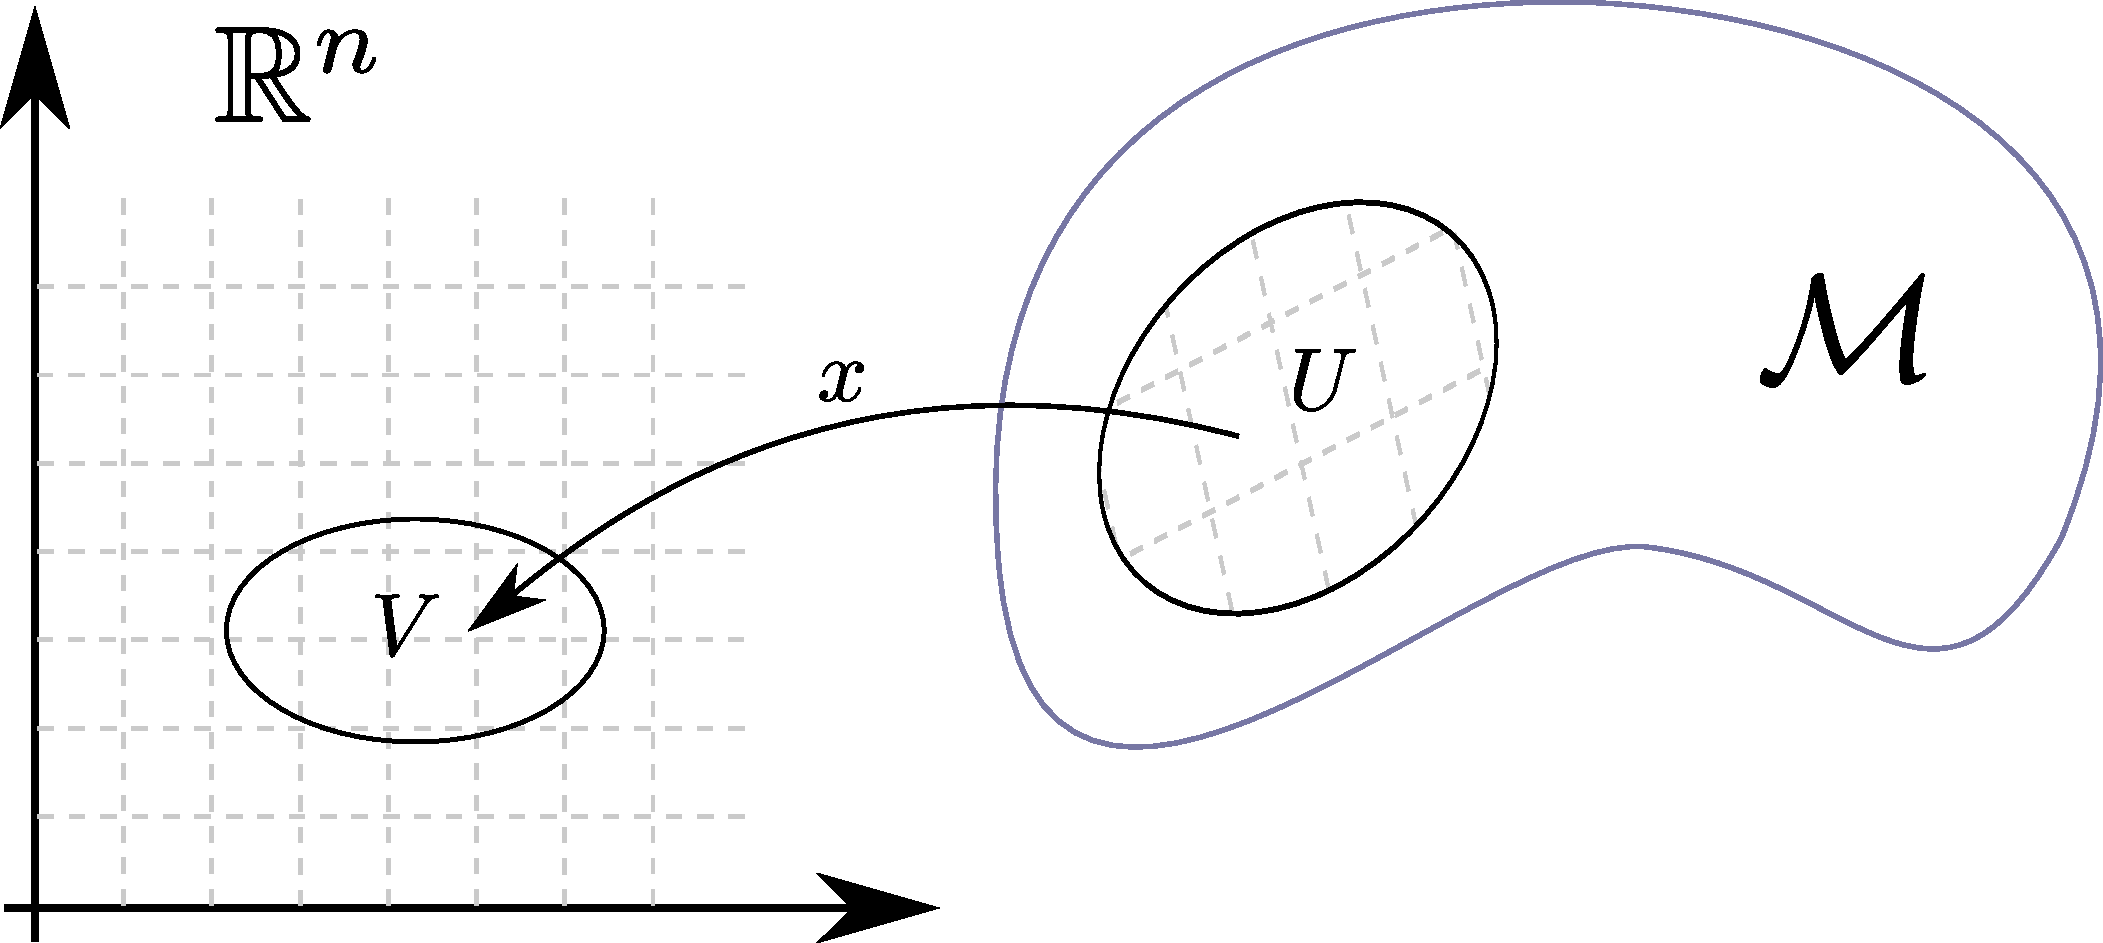
\includegraphics[width=0.7\textwidth]{figurer/coordinate_function.pdf}
    \label{coordinate function}
    \caption{The coordinate function $x$ maps a neighborhood $U$ in the manifold $\Em$ to a negiborhood $V$ in $\R^n$.}
\end{figure}

The most important objects in differential geometry are \emph{smooth manifolds}.
An $n$-dimensional manifold, $\Em$, is a set of points, locally homeomorphic to $\R^n$.
That is, for all points $p \in \Em$, there exists a neighborhood $U$ around $p$, together with a corresponding set of continuous, bijective functions,
%
\begin{align}
    x: U \subseteq \Em & \longmapsto V \subseteq \R^n, \\
    p & \longmapsto x^\mu(p).
\end{align}
%
We call $x(p) = (x^0(p), \dots, x^{n- 1}(p)) = x^\mu(p)$ a coordinate function of $\Em$.
The inverse of $x$, $x^{-1}$, obeys $x^{-1}(x(p)) = p$, for all $p \in U$.
A smooth manifold is one in which the coordinate functions are infinitely differentiable.
To define differentiability on manifolds, consider two coordinate functions, $x$, and $x'$.
The corresponding domains $U$ and $U'$ may or may not overlap.
We then define the transition function, a function between subsets of $\R^n$ by mapping via $\Em$, as
%
\begin{align}
    f_{x\rightarrow x'} = x' \circ x^{-1} : \R^n \mapsto \R^n.
\end{align}
%
The map is illustrated in \autoref{fig: transition map}.
\footnote{To be rigorous, one has to restrict the domains and image of the coordinate function when combining them. This is illustrated in \autoref{fig: transition map}.}
A set of coordinate functions $\mathcal A = \{x_i\}$ whose domain cover $\Em$ is called an \emph{atlas} of $\Em$.
If the transition function between all pairings of coordinate functions in the atlas is smooth---that is, infinitely differentiable---we call the atlas smooth.
We then define a smooth manifold as the topological manifold $\Em$ together with a \emph{maximal} smooth atlas $\mathcal A$.
A smooth atlas is maximal if no coordinate function can be added while the atlas remains smooth.\footnote{%
    The maximal condition ensres that two equivalent atlases correspond to the same differentiable manifold. A single manifold can be combined with different maximal atlases of smooth coordinates or differentiable structures. A set of examples are \emph{exotic spheres}, smooth manifolds which are \emph{homeomorphic} to $\text S^n$, but not \emph{diffeomorphic}. 
    }
%
\begin{figure}[H]
    \centering
    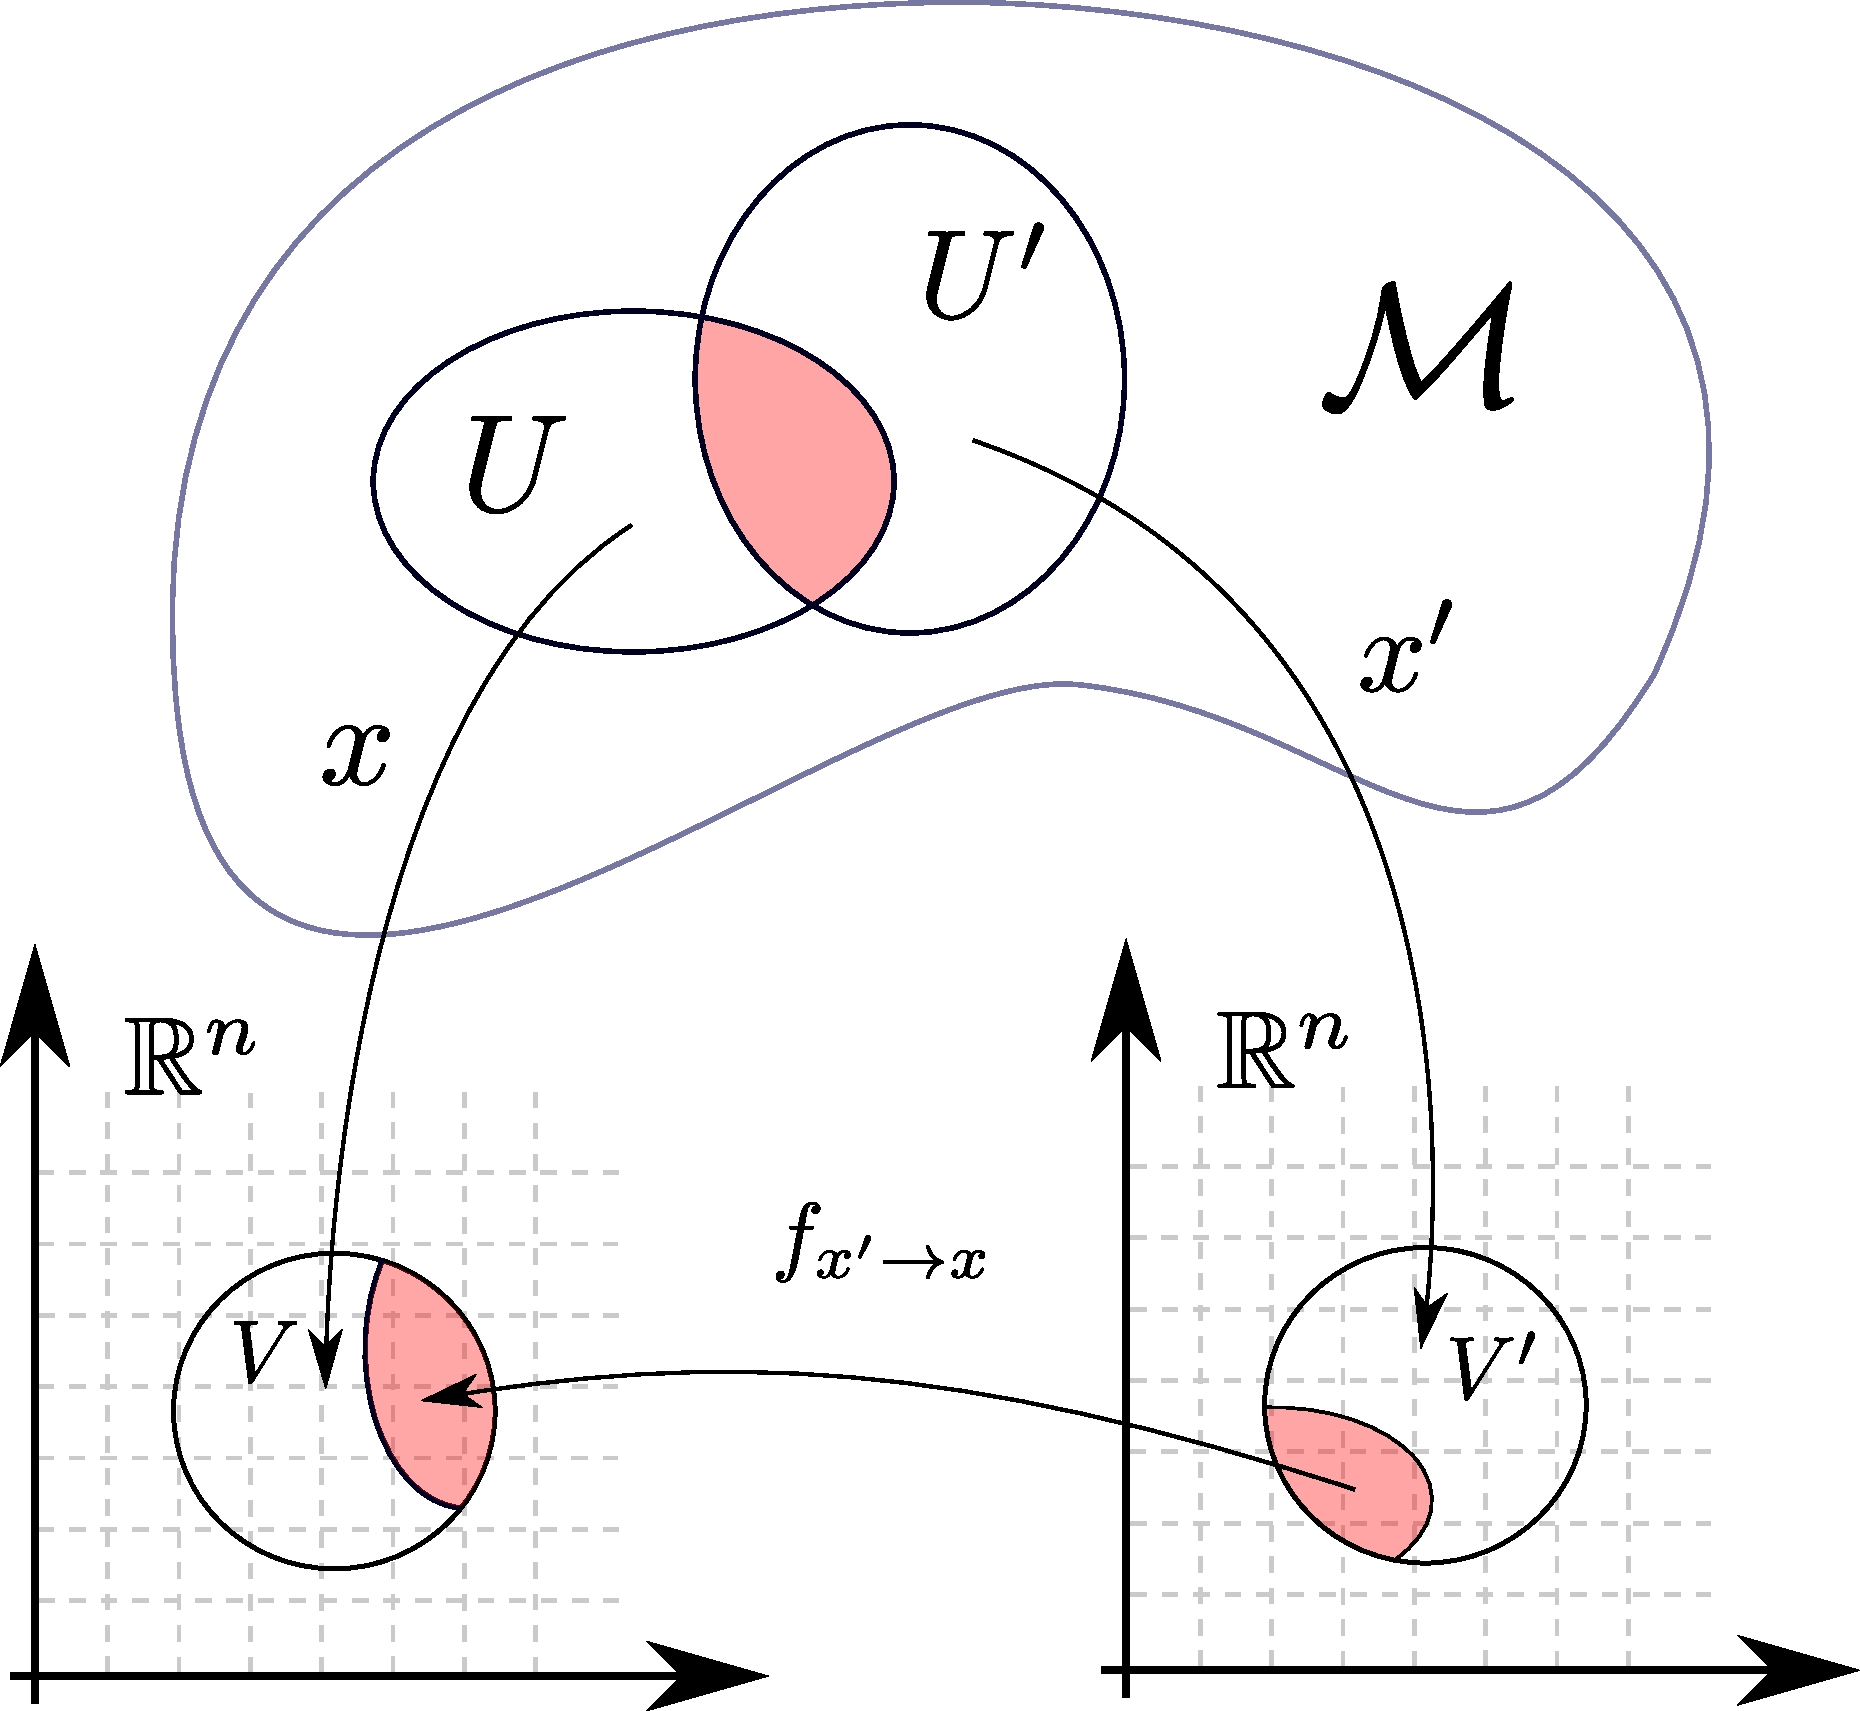
\includegraphics[width=0.6\textwidth]{figurer/transition_map.pdf}
    \caption{
        The transition map $f_{x'\rightarrow x}$ between two coordinate functions, $x$ and $x'$, maps between the images of these function, via the manifold $\Em$. 
        The function's domain and image are restricted to a (possibly empty) subset of the images of $x$ and $x'$. This is illustrated by the shaded regions in $V$ and $V'$. 
        }
    \label{fig: transition map}
\end{figure}

Consider two $m$- and $n$-dimensional smooth manifolds $\Em$ and $\mathcal N$.
Let $x$ denoted the coordinates on $\Em$, while $y$ denotes the coordinates on $\mathcal N$.
We can define smooth functions between these manifolds similarly to how we define smooth coordinates.
Consider the function
%
\begin{equation}
    F: \Em \longmapsto \mathcal N.
\end{equation}
%
It is said to be smooth if, for all points $p \in M$, there is a set of local coordinates $x$ around $p$ and $y$ around $F(p)$ such that the map $\tilde F = y \circ F \circ x^{-1}$ is smooth.
This map may be illustrated by a diagram,
%
\begin{equation}
    % https://tikzcd.yichuanshen.de/#N4Igdg9gJgpgziAXAbVABwnAlgFyxMJZABgBoBGAXVJADcBDAGwFcYkQAdDgW3pwAsARoIAEAJQB63EAF9S6TLnyEUZYtTpNW7LrwEBjJiICys+SAzY8BIuVLqaDFm0SceffocYiAcmYVWyrYUGk7arroewuIShDIaMFAA5vBEoABmAE4Q0oh2IDgQSGQgjPSCMIwACorWKqUw6TggjlouIAAe-iBZOUj5hUgATK3O7OndvbkjBUWIAMyj4SAAnpPZuSWDC0vtSbKUMkA
\begin{tikzcd}
    \mathcal M \arrow[d, "x"] \arrow[r, "F"] & \mathcal N \arrow[d, "y"] \\
    \mathbb R^m \arrow[r, "\tilde F"]               & \mathbb R^n              
    \end{tikzcd}
    %
\end{equation}
%
%
We will not be careful with the distinction between $F$, the function between the abstract manifolds, and $\tilde F$, the function of their coordinates, but rather denote both by $F(x)$.
We may take the partial derivative of such a function with respect to the coordinates $x$, $\pdv{F}/{x^\mu}$.
However, this is dependent on our choice of coordinates, as a set of local coordinates can always be scaled arbitrarily.
Any physical theory must be independent of our choice of coordinates, so our next task is to define the properties of a smooth manifold in a coordinate independent way.


\subsection{Vectors and tensors}

A curve $\gamma$ through $\Em$ is a function from $\R$ to $\Em$,
%
\begin{align}
    \gamma : \R &\longmapsto \Em \\
    \lambda & \longmapsto \gamma(\lambda).
\end{align}
%
Such curves are often denoted only by their coordinates and the parameter $\lambda$, $x^\mu(\lambda) = (x^\mu \circ \gamma)(\lambda)$.
With this curve, we can take the directional derivative of a real-valued function on the manifold, $f: \Em \mapsto \R$.
Assume $\gamma(\lambda = 0) = p$.
As we are always taking the derivative of functions between $\R^n$, for different $n$, we can use the chain rule.
The directional derivative of $f$ at $p$, given by this curve $\gamma$, is then
%
\begin{equation}
    \odv{}{\lambda} f(x(\lambda)) \bigg |_p = \odv{x^\mu}{\lambda} \bigg |_{\lambda = 0}  \pdv{}{x^\mu} f(x) \bigg |_p.
\end{equation}
%
The set of all such directional derivatives, $\odv{}/{\lambda}$ at $p$, form a vector space, $T_p \Em$, called the \emph{tangent space}.
The tangent space is illustrated in \autoref{fig: tangent space}.
The coordinates $x^\mu$ induce a basis of this vector space, namely partial derivatives with respect to the coordinate functions at $p$
%
\begin{equation}
    e_\mu = \pdv{}{x^\mu} \bigg|_p = \partial_\mu|_p, \quad \mu \in \{0, ... n-1\}.
\end{equation}
%
Any element $v \in T_p \Em$ can therefore be written
%
\begin{equation}
    v = v^\mu \partial_\mu |_p = \odv{x^\mu}{\lambda}\Big |_{\lambda = 0} \pdv{}{x^\mu}\Big |_p.
\end{equation}
%
Here, $\lambda$ is the parameter of the curve corresponding to the directional derivative $v$.\footnote{%
There is not only one curve corresponding to any directional derivative but rather an equivalence class. We will gloss over this technicality, as it does not affect our work.
}
The evaluation at $\lambda = 0$ and $p$ will often be implicit for ease of notation.
This directional derivative acts on functions $f : \Em \mapsto \R$ as
%
\begin{equation}
    v(f) = v^\mu \partial_\mu f.
\end{equation}
%

\begin{figure}[ht]
    \centering
    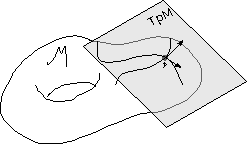
\includegraphics[width=0.7\textwidth]{figurer/tangent space.pdf} 
    \caption{
        (Kladd) The tangent space $T_p \Em$, the shaded rectangle, is the sett of all directional derivatives at $p\in \Em$. A directional derivative is defined in terms of a curve that passes through $p$.
        } 
    \label{fig: tangent space}
\end{figure}



A map $F$ between two manifolds $\Em$ and $\mathcal N$ also induces a map between the tangent spaces of these manifolds.
This is the \emph{differential} of $F$ at $p$, 
%
\begin{align}
    \dd F_p: T_p \Em & \longmapsto T_p \mathcal N, \\
    v & \longmapsto \dd F_p (v). 
\end{align}
%
As $\dd F_p(v)$ is an element of $T_p \mathcal N$,   directional derivative on $\mathcal N$, defined as
%
\begin{equation}
    \dd F_p(v) (g) = v(g \circ F),
\end{equation}
%
for functions $g : \mathcal N \mapsto \R$.
It thus acts on functions on $\mathcal N$ by ``extending'' the derivative $v$.
This is a linear map between vector spaces and may be written in component form by considering the differentials of the coordinate functions.
Denote the coordinates of $\mathcal N$ by $y^\mu$, and $y^\mu \circ F = F^\mu$.
Then,
%
\begin{equation}
    \dd F_p (\partial_\mu) (g) = \partial_\mu (g \circ F) |_p 
    = \pdv{F^\nu}{x^\mu}\Big |_p \pdv{g}{y^\nu} \Big  |_{F(p)},
\end{equation}
%
or more suggestively
%
\begin{equation}
    \dd F \left( \pdv{}{x^\mu} \right) = \pdv{F^\nu}{x^\mu} \pdv{}{y_\nu}.
\end{equation}
%
This is a linear map of vectors between two vectors by the matrix $A_\mu{}^\nu = \partial_\mu F^\nu$.
The differential is thus a generalization of the Jacobian.
In the case of a real valued function, $f: \Em \mapsto \R$, and $g : \R \mapsto \R$, we get
%
\begin{equation}
    \dd f (v) (g) 
    = v(g \circ f) 
    = (v^\mu \partial_\mu f) \, \odv{g}{y}.
\end{equation}
%
$\dd f$ is thus a map from $T_p \Em$ to $T_{f(p)}\R$, which is isomorphic to $\R$.
The $g$ be the identity function, so that $\odv{g}/{y} = 1$.
Then, the differential of a scalar function, also called a 1-form, is a map from vectors $v$ to real numbers,
%
\begin{equation}
    \label{covectors i.e. one forms}
    \dd f(v) := v^\mu \partial_\mu f.
\end{equation}
%
The set of all linear maps from a vector space $V$ to the real numbers is called the \emph{dual space} of $V$, denoted $V^*$.
This is a new vector space with the same dimensionality as $V$.
We denote the dual of $T_p \Em$ as $T_p^* \Em$.
We can regard each coordinate function as a real-valued function with a corresponding differential.
This differential obeys
%
\begin{equation}
    \dd x^\mu (\partial_\nu) = \pdv{x^\mu}{x_\nu} = \delta^\mu_\nu.
\end{equation}
%
The differentials of the coordinate functions thus form a basis for $T^*_p \Em$, called the dual basis.
Any differential $\dd f$ can thus be written as $\dd f = \omega_\mu \dd x^\nu$ for some components $\omega_\mu$.
We finde the components by applying the differential to the coordinate basis, $\dd f(\partial_\mu) = \partial_\mu f = \omega_\mu$.
In other words, we recover the classical expression 
%
\begin{equation}
    \dd f = \pdv{f}{x^\mu} \dd x^\mu,
\end{equation}
however we now interpret it as a covector-field instead of an ``infinitesimal displacement''.

Linear maps from vectors to real numbers is generalized by \emph{tensors}.
Given a vector space $V$, a general $(n, m)$ tensor $T$ is a multilinear map, which associates $n$ elements from $V$ and $m$ from its dual $V^*$ to the real numbers, i.e.,
%
\begin{align}
    T: V \times V \times \dots\times V^* \times \dots &\longmapsto \R, \\
    (v, u\dots; \omega, \dots) & \longmapsto T(v, u, \dots; \omega, \dots).
\end{align}
%
Multilinear means that $T$ is linear in each argument.
The set of all such maps is the tensor product space $V\otimes V \otimes \dots \otimes V^* \otimes \dots$, a $\dim(V)^{n+m}$-dimensional vector space.
If $\{e_\mu\}$ and $\{e^\mu\}$ are the basis for $V$ and $V^*$, then we can write the basis of this of the tensor product space as $ \{e_{\mu} \otimes\dots \otimes e^{\nu} \otimes \dots \}$.
The tensor can thus be written
%
\begin{equation}
    T =
     T^{\mu \nu\dots}{}_{\rho\dots} \, e_{\mu}\otimes e_\nu \otimes \dots e^\rho\otimes\dots, \quad
    T^{\mu \nu\dots}{}_{\rho\dots} = T(e^\mu, e^\nu, \dots; e_\rho, \dots).
\end{equation}
% 
We often what to decopose a tensor down into its symmetric and antisymmetric parts.
To do this, we introduce the symmetrization of a tensor $T$, 
%
\begin{equation}
    T_{(\mu_1\dots\mu_n)} 
    = \frac{1}{n!} \sum_{\sigma \in S_n} 
    T_{\mu_{\sigma(1)} \dots \mu_{\sigma(n)}},
\end{equation}
%
where $S_n$ is the set of all permutations of $n$ objects.
The antisymmetrization of a tensor is defined as
%
\begin{equation}
    T_{[\mu_1\dots\mu_n]} 
    = \frac{1}{n!} \sum_{\sigma \in S_n} \text{sgn}(\sigma)  
    T_{\mu_{\sigma(1)} \dots\mu_{\sigma(n)}}.
\end{equation}
%
The function $\text{\sigma} = \pm 1$, depending on if $\sigma$ is a even or odd permutation.
We may now write
%
\begin{equation}
    T_{\mu \nu} = T_{(\mu \nu)} + T_{[\mu \nu]}.
\end{equation}


\subsection{Geometry and the metric}
\label{subsection: goemetry and the metric}

The metric is a symmetric, non-degenerate $(0, 2)$ tensor
%
\begin{equation}
    \dd s^2 = g_{\mu \nu} \, \dd x^\mu \otimes \dd x^\nu.
\end{equation}
%
It defines the geometry of the manifold $\Em$, and is the main object of study in general relativity.
As it is invertible, we can define $g^{\mu \nu} = (g^{-1})_{\mu \nu}$, which is the components of a $(2, 0)$ tensor.
We use this to raise and lower indices, as is done with the Minkowski metric $\eta_{\mu \nu}$ in special relativity.

Up until now, we have only considered the tangent space $T_p \Em$ at a point $p$ and the corresponding tensor-product spaces.
We are, however, more interested in \emph{fields} of vectors, covectors, or tensors.
For each point $p \in \Em$, a tensor field $T$ ``picks out'' a tensor $T(p)$ from each tensor product space corresponding to the tangent space at $p$, $T_p \Em$.
We will use a vector field to illustrate.
This vector field can be written as
%
\begin{equation}
    v(p) = v^\mu(p) \partial_\mu |_p. 
\end{equation}
%
We will mostly be working with the components $v^\mu$, which are functions of $\Em$.
For ease of notation, we write the vector as a function of the coordinates $x$.
The vector field $v(x)$ is unchanged by a coordinate-transformation $x^\mu \rightarrow {x'}^\mu$; the coordinates are only a tool for our convenience.
However, with a new set of coordinates, we get a new set of basis vectors, $\partial'_\mu$:
%
\begin{equation}
    v = v^\mu \partial_\mu = v^\mu \pdv{x'^\nu}{x^\mu} \partial'_\nu
    = v'^\mu \partial_\mu',
\end{equation}
%
This gives us the transformation rules for the components of vectors,
%
\begin{equation}
    v'^\mu = \pdv{x'^\mu}{x^\nu} v^\nu.
\end{equation}
%
Tangent vectors are also called \emph{contravariant} vectors, as their components transform contra to basis vectors.
For covectors, it is
%
\begin{equation}
    \omega'_\mu = \pdv{x^\nu}{x'^\mu} \omega_\nu,
\end{equation}
%
which is why covectors also are called \emph{covariant} vectors.

The gradient of a scalar function $f$, $\dd f = \partial_\mu f \dd x^\mu$, is a coordinate-independent derivative, as $\partial_\mu f$ follows the transformation law for covectors.
We define the covariant derivative, $\nabla$, as a map from $(n, m)$ tensor fields to $(n, m+1)$ tensor fields.
When considering a scalar as a $(0, 0)$ tensor, we see that this generalizes the scalar derivative.
The components of a covariant derivative, $\nabla_\rho T^{\mu_1\dots}{}_{\nu_1, \dots}$, must follow the tensor transformation law. 
However, this is not strong enough to uniquely define $\nabla$.
We further assume
%
\begin{itemize}
    \item Linearity: $\nabla (T + S) = \nabla T + \nabla S$.
    \item The product rule: $\nabla (T \otimes S) = (\nabla T)\otimes S + T \otimes (\nabla S)$.
    \item Reduces to partial derivative for scalars: $\nabla_\mu f = \partial_\mu f$.
    \item Kronecker delta gives zero: $\nabla_\mu \delta^\rho_\nu = 0$.
\end{itemize}
%
With this, we can, in general, write the covariant derivative as~\autocite{carrollSpacetimeGeometryIntroduction2019}
%
\begin{align}
    \label{covariant derivative diff geom}
    \nabla_\mu v^\nu &= \partial_\mu v^\nu + \Gamma^\mu_{\nu \rho} v^\rho, \\
    \label{covariant derivative diff geom covector}
    \nabla_\mu \omega_\nu &= \partial_\mu \omega_\nu - \Gamma^\rho_{\mu \nu} \omega_\rho,
\end{align}
%
for vectors and covectors.
$\Gamma^{\mu}_{\nu \rho}$ are called \emph{Christoffel symbols}.
The generalization for higher-order tensors is straightforward, 
%
\begin{equation}
    \nabla_\mu T^{\nu\dots}{}_{\rho\dots}
    =
    \partial_\mu T^{\nu\dots}{}_{\rho\dots}
    + \Gamma^\mu_{\nu \lambda} T^{\lambda\dots}{}_{\rho\dots} +\dots
    - \Gamma^\lambda_{\mu \rho} T^{\mu\dots}{}_{\lambda\dots} -\dots.
\end{equation} 
%
This is still not enough to uniquely determine the covariant derivative.
We will furthermore assume $\Gamma^{\lambda}_{\mu \nu} = \Gamma^{\lambda}_{\nu \mu}$ and $\nabla_\mu g_{\nu \rho} = 0$.
With these, we can find an explicit formula of the Christoffel symbols in terms of the metric,
%
\begin{equation}
    \label{christoffel symbols from metric}
    \Gamma^\rho_{\mu \nu} = \frac{1}{2} g^{\rho \sigma} (\partial_\mu g_{\nu \sigma} - \partial_\sigma g_{\mu \nu} + \partial_{\nu}g_{\sigma \mu}).
\end{equation}
%
With the notion of a covariant derivative, we may also generalize \emph{parallel transport} to curved spaces.
The notion of parallel transport of a vector in flat $\R^n$ is intuitive---given a line $x^\mu(\lambda)$, a vector $v^\mu$ at $x^\mu(\lambda_0)$ is parallel transported to $v'^\mu$ at $x^\mu(\lambda_1)$ if they ``point in the same direction''.
To make this more precise, a vector field $v^\mu$ is parallel transported along $x^\mu(\lambda)$ if $\odv{}{\lambda} v^\mu = \odv{x^\nu}{\lambda} \partial_\nu v^\mu$ = 0.
We generalize this to curved spaces by replacing the partial derivative with a covariant derivative, and so the criterion for parallel transport is
%
\begin{equation}
    \label{parallel transport criterion}
    \odv{x^\mu}{\lambda} \nabla_\mu v^\nu = 0.
\end{equation}
%
With this, we can imagine creating a special class of paths, called \emph{geodesics}, namely those which parallel transport their tangent vectors $\odv{x^\mu}{\lambda}$.
We imagine following an arrow we are holding without turning it as we walk.
Using the definition of parallel transport \autoref{parallel transport criterion}, together with the covariant derivative \autoref{covariant derivative diff geom}, we get the geodesic equation,
%
\begin{equation}
    \label{goedesic equation}
    \odv[2]{x^\mu}{\lambda} 
    + \Gamma^\mu_{\rho \sigma} \odv{x^\rho}{\lambda} \odv{x^\rho}{\lambda}
    = 0.
\end{equation}
In a flat space, where the Christoffel symbols vanish, this reduces to the familiar criterion for straight lines, $\odv[2]{x^\mu}{\lambda} = 0$.

The curvature of a manifold $\Em$, with the metric $g_{\mu \nu}$, is encoded in the Riemann tensor.
It is defined by
%
\begin{equation}
    \label{Riemann tensor}
    [\nabla_\mu, \nabla_\nu] v^\rho = R^{\rho}{}_{\sigma \mu \nu} v^\sigma,
\end{equation}
%
which in our case gives the explicit formula
%
\begin{equation}
    \label{riemann tensor in terms of christoffel symbols}
    R^\rho{}_{\sigma \mu \nu} 
    = \partial_{\mu} \Gamma^{\rho}_{\nu \sigma}
    - \partial_{\nu} \Gamma^{\rho}_{\mu \sigma}
    + \Gamma^{\rho}_{\mu \lambda} \Gamma^{\lambda}_{\nu \sigma}  
    - \Gamma^{\rho}_{\nu \lambda} \Gamma^{\lambda}_{\mu \sigma}.
\end{equation}
%
Although the Christoffel symbols are not tensors, the Riemann tensor is due to its definition using covariant derivatives.
We can therefore contract some of its indices to get other tensor quantities.
We  efine the Ricci tensor and Ricci scalar as
%
\begin{align}
    \label{Ricci tensor}
    R_{\mu \nu} &= R^{\rho}{}_{\mu \rho \nu}, \\
    \label{Ricci scalar}
    R &= R^{\mu}{}_{\mu} = g^{\mu \nu} R_{\mu \nu}.
\end{align}
%
This form gives us several useful identities, such as
%
\begin{equation}
    R_{\rho \sigma \mu \nu} 
    = 
    R_{[\rho \sigma] \mu \nu}
    =
    R_{\rho \sigma [\mu \nu]}
    =
    R_{\mu \nu \rho \sigma }.
\end{equation}
%
Using the Jacobi identity of the commutator, we have
%
\begin{equation}
    \label{Jacobi identity differential geometry}
    [\nabla_\mu, [\nabla_\nu, \nabla_\sigma]]
    + [\nabla_\sigma, [\nabla_\mu, \nabla_\nu]]
    + [\nabla_\nu, [\nabla_\sigma, \nabla_\mu]] = 0.
\end{equation}
%
If we apply this on $\delta^{\mu}_{\nu}$, we get the differential Bianchi identity, compactly written
%
\begin{equation}
    \label{Binachi identiy}
    \nabla_{[\mu}R_{\nu \rho]\sigma \eta} = 0.
\end{equation}
%
To interpret the Riemann tensor, we define the parallel propagator $P$.
A vector that is parallel transported along a curve parametrized by $\lambda$, so that $v^\mu(\lambda)$ obey the criterion of parallel transport \autoref{parallel transport criterion}, obey
%
\begin{equation}
    v^\mu(\lambda) = P^\mu{}_\nu(\lambda) v^\nu.
\end{equation}
%
Inserting this into the equation for parallel transport, \autoref{parallel transport criterion}, this operator must obey
%
\begin{equation}
    \odv{}{\lambda} P^\mu{}_\nu = - \Gamma^\mu_{\rho \sigma}  \odv{x^\rho}{\lambda}P^\sigma{}_\nu.
\end{equation}
%
This has the same form as the definition of the unitary time-evolution operator in quantum mechanics, and we could therefore write down a solution involving an exponential and a path ordering operator, $\mathcal P$, analogous to the time ordering operator from quantum mechanics.
We may rewrite the equation as an integral equation,
%
\begin{equation}
    P^\mu{}_\nu(\lambda) = \delta^\mu_\nu 
    - \int^\lambda_0 \dd \lambda' \Gamma^\mu_{\rho \sigma} V^\rho P^\sigma{}_\nu,
\end{equation}
%
where we denote $\odv{x^\mu}{\lambda} = V^\mu$.
This allows us to solve the equation iteratively.
If $\lambda \leq \epsilon \ll 1$, then we would expect this to converge, as long as the $g$ is well-behaved.
In that case, we can start with the zeroth-order solution $P^{\mu}{}_\nu = \delta^\mu_\nu$, then iterate twice to obtain
%
\begin{equation}
    \label{iterative paralell propagator}
    P^\mu{}_\nu(\lambda) 
    = 
    \delta^\mu_\nu 
    - \int_0^\lambda \dd \lambda' \, 
    \Gamma^\mu_{\rho \nu} V^\rho
    + \int_0^{\lambda} \dd \lambda ' \int_0^{\lambda'} \dd \lambda ''\,
    \Gamma^\mu_{\rho \sigma} \Gamma^\sigma_{\eta \nu} V^\rho V^\eta
    + \Oh(\epsilon^3).
\end{equation}
%
With this, we will investigate how much a vector $v^\mu$ is changed by being parallel transported around in a small loop.
This is illustrated in \autoref{fig: parallel transport in loop}.
%
\begin{figure}
    \centering
    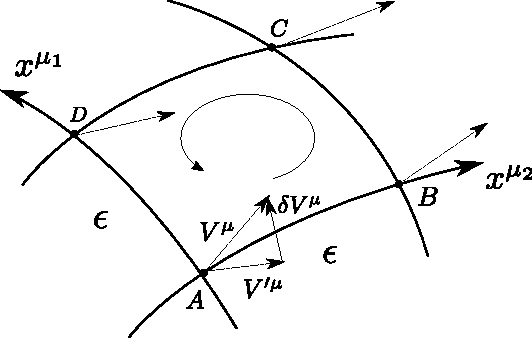
\includegraphics[width=0.7\textwidth]{figurer/parallel_transport.pdf}
    \caption{A vector $v^\mu$ is parallel transported in a small, closed loop, defined by the coordinate functions $x^{\mu_1}$ and $x^{\mu_2}$.
    As a consequence of the curvature, it has changed by $\delta v^\mu$ by the time it arrives back at $A$.}
    \label{fig: parallel transport in loop}
\end{figure}
%
A vector $v^\mu$, is parallel transported in a loop along the coordinate lines.
These lines are where either of the coordinate functions $x^{\mu_1}$ or $x^{\mu_2}$ are equal to $0$ or $\epsilon$.
Here, the indices $\mu_1$ and $\mu_2$ are not free, but identify the two coordinate functions which define this loop.
The line from $A$ to $B$, defined by $x^{\mu_1} = 0$, is parametrized by $x^\mu(\lambda) = \lambda \delta^\mu_{\mu_2}$, so $ V^\mu = \delta^\mu_{\mu_2} $.
The Christoffel symbol along this line is
%
\begin{equation}
    \Gamma^{\mu}_{\nu \rho}(\lambda) 
    = \Gamma^{\mu}_{\nu \rho}|_A
    + \lambda \partial_{\mu_2} \Gamma^{\mu}_{\nu \rho}|_A + \Oh(\lambda^2).
\end{equation}
%
Inserting this into \autoref{iterative paralell propagator}, we get
%
\begin{equation}
    P^\mu{}_\nu(\epsilon)
    = \delta^\mu_\nu 
    - \epsilon \Gamma^{\mu}_{\nu \mu_2}|_A
    + \frac{1}{2} \epsilon^2 
    \left(
        \Gamma^\mu_{\mu_2 \sigma}\Gamma^\sigma_{\mu_2 \nu} |_A 
        -\partial_{\mu_2} \Gamma^{\mu}_{\nu \mu_2}|_A 
    \right)
    + \Oh(\epsilon^3).
\end{equation}
%
Next, from $B$ to $C$, the line is $x^\mu(\lambda) = \epsilon \delta^\mu_{\mu_2} + \lambda \delta^{\mu}_{\mu_1}$, so $V^\mu = \delta^\mu_{\mu_1}$, and the Christoffel symbols are 
$ 
\Gamma^{\mu}_{\nu\rho}
= 
\Gamma^{\mu}_{\nu \rho}|_B
+ \lambda \partial_{\mu_1} \Gamma^{\mu}_{\nu \rho}|_B
$
to fist order in $\lambda$.
Here, we have to expand once more to evaluate the symbols at $A$.
Then, we get
%
\begin{equation}
    \Gamma^{\mu}_{\nu\rho}
    =
    \Gamma^{\mu}_{\nu \rho}|_A + \epsilon \partial_{\mu_2} \Gamma^{\mu}_{\nu \rho}|_A
    + \lambda \partial_{\mu_1} \Gamma^{\mu}_{\nu \rho}|_A,
\end{equation}
%
The parallel propagator from $B$ to $C$ is then
%
\begin{equation}
    P^{\mu}{}_\nu(\epsilon)
    = 
    \delta^\mu_\nu
    - \epsilon \Gamma^{\mu}_{\nu \mu_1}|_A 
    + \frac{1}{2}\epsilon^2
    \left(
        \Gamma^\mu_{\sigma \mu_1}\Gamma^\sigma_{\nu \mu_1}|_A
        - \partial_{\mu_1} \Gamma^{\mu}_{\nu \mu_1}|_A
        - 2 \partial_{\mu_2} \Gamma^{\mu}_{\nu \mu_1}|_A
    \right).
\end{equation}
%
The combined propagator from $A$ to $C$ is then, to second order in $\epsilon$, 
%
\begin{align}
    \nonumber
    {P_{AC}}^\mu{}_{\nu}
    & = 
    \left[ 
        \delta^\mu_\sigma 
        -\epsilon \Gamma^{\mu}_{\sigma \mu_1}
        + \frac{1}{2} \epsilon^2 
        \left(
        \Gamma^\mu_{\eta \mu_1}\Gamma^\eta_{\sigma \mu_1}
        - \partial_{\mu_2} \Gamma^{\mu}_{\sigma \mu_2}
        - 2 \partial_{\mu_2} \Gamma^{\mu}_{\sigma \mu_1}
        \right)
    \right]
    \cdot 
    \left[
        \delta^\sigma_\nu
        - \epsilon \Gamma^{\sigma}_{\nu \mu_2}
        + \frac{1}{2} \epsilon^2 
        \left(
            \Gamma^\sigma_{\eta \mu_2}\Gamma^\eta_{\nu \mu_2}
            - \partial_{\mu_2} \Gamma^{\sigma}_{\nu \mu_2}
        \right)
    \right] \\ \nonumber
    & =
    \delta^\mu_\nu
    - \epsilon 
    \left(
        \Gamma^{\mu}_{\nu \mu_1}
        +
        \Gamma^{\mu}_{\nu \mu_2}
    \right)
    + \epsilon^2
    \frac{1}{2}
    \left(  
        2\Gamma^{\mu}_{\sigma \mu_1} \Gamma^{\sigma}_{\nu \mu_2}
        + \Gamma^\mu_{\sigma \mu_1}\Gamma^\sigma_{\nu \mu_1}
        + \Gamma^\mu_{\sigma \mu_2}\Gamma^\sigma_{\nu \mu_2}
        - 2 \partial_{\mu_2} \Gamma^{\mu}_{\nu \mu_1}
        - \partial_{\mu_1} \Gamma^{\mu}_{\nu \mu_1}
        - \partial_{\mu_2} \Gamma^{\mu}_{\nu \mu_2}
    \right).
\end{align}
%
The parallel propagator for $CDA$ is the propagator for $ADC$ with its signs flipped. 
The $ADC$ propagator is the same as $ABC$, only with the $\mu_1$ and $\mu_2$ indices switched.
It is thus
%
\begin{align}
    \nonumber
    {P_{CA}}^\mu{}_\nu
    & =
    \delta^\mu_\nu
    + \epsilon 
    \left(
        \Gamma^{\mu}_{\nu \mu_2}
        +
        \Gamma^{\mu}_{\nu \mu_1}
    \right)
    + \epsilon^2
    \frac{1}{2}
    \left(  
        2\Gamma^{\mu}_{\sigma \mu_2} \Gamma^{\sigma}_{\nu \mu_1}
        + \Gamma^\mu_{\sigma \mu_2}\Gamma^\sigma_{\nu \mu_2}
        + \Gamma^\mu_{\sigma \mu_1}\Gamma^\sigma_{\nu \mu_1}
        + 2 \partial_{\mu_1} \Gamma^{\mu}_{\nu \mu_2}
        + \partial_{\mu_2} \Gamma^{\mu}_{\nu \mu_2}
        + \partial_{\mu_1} \Gamma^{\mu}_{\nu \mu_1}
    \right).
\end{align}
%
The full propagator, from $A$ to $A$, is $P^\mu{}_\nu = {P_{CA}}^\mu{}_\rho {P_{AC}}^\rho{}_\nu$.
The terms linear in $\epsilon$ vanish, and the same with the terms with two equal $\mu_i$-indices.
The change in the vector as it is rotated around the loop is therefore, to second order in $\epsilon$,
%
\begin{align}
    \delta v^\mu 
    = P^\mu{}_\nu v^\nu - v^\mu 
    = \epsilon^2  
    \left(
        \Gamma^\mu_{\sigma \mu_1} \Gamma^\sigma_{\nu \mu_2}
        -\Gamma^\mu_{\sigma \mu_2} \Gamma^\sigma_{\nu \mu_1}
        + \partial_{\mu_1} \Gamma^{\mu}_{\nu \mu_2}
        - \partial_{\mu_2} \Gamma^{\mu}_{\nu \mu_1} 
    \right) v^\nu.
\end{align}
Comparing with \autoref{riemann tensor in terms of christoffel symbols}, we see that this is the Riemann curvature tensor.
In other words, the Riemann tensor encodes how a vector is transformed when parallel transported in a small, closed loop.



\subsection{Integration on manifolds}
\label{subsection: integration on manifolds}

The integral of a scalar function on a manifold is not a coordinate-independent notion, and we must introduce the notion of $n$-forms.
A $n$-form is a antisymmetric $(0, n)$ tensor.
The wedge product, $\wedge$ is a product which maps two $n$- and $m$-forms to a $n+m$-form, and is defined as
%
\begin{equation}
    (A\wedge B)_{\mu_1\dots\mu_{n+m}} = \frac{(n + m)!}{n! m!} A_{[\mu_1\dots\mu_n}B_{\mu_{n+1}\dots\mu_{n+m}]},
\end{equation}
%
A $n$-form $\omega$ may now be written as
%
\begin{equation}
    \omega 
    = \omega_{[\mu_1 \dots \mu_n]} \, \dd x^{\mu_1} \otimes \dots \otimes \dd x^{\mu_n}
    = \omega_{\mu_1 \dots \mu_n} \, \dd x^{\mu_1} \wedge \dots \wedge \dd x^{\mu_n}.
\end{equation}
% 
Furthermore, we define the exterior derivative, a map from $n$-forms to $n+1$-forms, defined by
%
\begin{equation}
    (\dd T)_{\mu_1 \dots \mu_{n+1}} = (n+1) \partial_{[\mu_1} T_{\mu_2\dots\mu_{n+1}]}.
\end{equation}
%
We are interested in a coordinated independent quantity that we can integrate over.
To that end, we define
%
\begin{equation}
    \dd^n x := \dd x^0 \wedge \dots \wedge \dd x^{n-1}
    = \frac{1}{n!} \varepsilon_{\mu_1 \dots \mu_n}  
    \dd x^{\mu_1} \wedge \dots \wedge \dd x^{\mu_n},
\end{equation}
%
Where $\varepsilon_{\mu_1 \dots \mu_n}$ is the Levi-Civita symbol.
Given a different set of coordinates, $x'^\mu$, these are related by
%
\begin{equation}
    \dd^n x = \det\left( \pdv{x}{x'} \right) \, \dd^n x',
\end{equation}
%
where we have used the relation $\varepsilon_{\mu_1 \dots \mu_n}  \det(A) = \varepsilon_{\nu_1 \dots \nu_n} A^{\nu_1}{}_{\mu_1} \dots A^{\nu_n}{}_{\mu_n}$.  
We define $|g| = |\det(g_{\mu \nu })|$, which, by the transformation properties of tensors, transforms as
%
\begin{equation}
    \sqrt{|g'|} = \left| \det\left(\pdv{x'}{x} \right) \right| \sqrt{|g'|},
\end{equation}
%
This means that we can use this to compensate for the transformation of $\dd^n x$, and get a volume form with a coordinate independent expression,
%
\begin{equation}
    \dd V = \sqrt{|g|} \, \dd^n x = \sqrt{|g'|} \, \dd^n x'.
\end{equation}
%
With this, we can integrate scalars in a well-defined way by mapping them to a corresponding $n$-form, $f \rightarrow f \dd V$.
We define the integral of a scalar function $f$ on a manifold $\Em$ with a metric $g$ as
%
\begin{equation}
    I = \int_\Em \dd V \, f =  \int_{\Em} \dd^n x \, \sqrt{|g(x)|} \, f(x).  
\end{equation}


Stoke's theorem generalizes the fundamental theorem of calculus and the divergence theorem to manifolds.
Let $\Em$ be a differential manifold of dimension $n$, with the boundary $\partial \Em$.
Stoke's theorem says that, for an $n-1$-form $\omega$,
%
\begin{equation}
    \int_\Em \dd \omega = \int_{\partial \Em}  \omega. 
\end{equation}

Stoke's theorem then implies a generalized divergence theorem.
The boundary of $\Em$ is a $n-1$ manifold dimensional, and a metric $g$ on $\Em$ will induce a new metric $\gamma$ on $\partial \Em$.
This metric corresponds to the restriction of $g$ to $\partial \Em$.
Furthermore, there will be a vector field $n^\mu$ of normalized vectors orthogonal to all elements of $T \partial \Em$.
This theorem states that for a vector field $V^\mu$ on $\Em$,
%
\begin{equation}
    \label{generalized divergence theorem}
    \int_\Em \dd^n x \, \sqrt{|g|} \,  \nabla_\mu V^\mu 
    = \int_{\partial \Em} \dd^{n-1}y \, \sqrt{|\gamma|} \, n_\mu V^\mu.
\end{equation}

    \section{*Lie groups}

This section is based on~\autocite{leeIntroductionSmoothManifolds2003d,peskinIntroductionQuantumField1995,schwartzQuantumFieldTheory2013,weinbergQuantumTheoryFields1995,weinbergQuantumTheoryFields1996}.


\subsection{Groups}
Lie groups are a natural structure to capture the symmetries of a physical theory.
A Lie group is a smooth manifold, with the additional structure of a \emph{group}.
A group is a set, $G$, together with a map
%
\begin{align}
    (\cdot, \cdot):  G \times G &\longmapsto G ,\\
    (g_1, g_2) &\longmapsto g_3,
\end{align}
% 
called group multiplication. This map obeys the group axioms, which are the existence of an identity element $\one$, associativity and the existence of an inverse element $g^{-1}$ for all $\in G$.
These can be written as
\begin{table}[!h]
    \centering
    \begin{tabular}{l l}
        $\forall g \in G, $&$ (g, \one) = g, $\\
        $\forall g_1, g_2, g_3 \in G, $ & $ (g_1, (g_2, g_3)) = ((g_1, g_2), g_3), $\\
        $\forall g \in G,\, \exists g^{-1} \in G,\, \text{s.t.}, $ & $ (g, g^{-1}) = \one.$
    \end{tabular}
\end{table}

In addition, we require that both the multiplication map and the inverse map, $g \mapsto g^{-1}$, are smooth.
As we will discuss later, a symmetry transformation is a map between physical states which leave the equations governing that system unchanged.
Assume the field, or set of fields, $\varphi$ is governed by the equation $f(\varphi) = 0$.
A symmetry transformation $\varphi \mapsto g \varphi$ will then obey $f(g\varphi) = 0$.
This is what makes groups the natural structures to describe symmetries.
Assume $G$ is the set of all, or a subset closed under compositions, symmetries of a system,
%
\begin{equation}
    G = \setbuilder{g}{f(g\varphi) = 0},
\end{equation}
%
as a Lie group.
The group $G$ might act on $\varphi$ linearly, so $(g\varphi)_i = g_{ij}\varphi_j$, or in a more complicated matter.
In this case, the group multiplication is composition, i.e., performing transformations in succession.
This map is closed, as the composite of two symmetry transformations is another symmetry transformation.
The identity map is a symmetry transformation, and composition is associative.
This means that invertible symmetry transformations form a group.

We will focus on connected Lie groups, in which all elements $g \in G$ are in the same connected piece as the identity map $\one \varphi = \varphi$.
This means that for each $g\in G$, one can find a continuous path $\gamma(t)$ in the manifold, such that $\gamma(0) = \one$ and $\gamma(1) = g$.
Given such a path, we can study transformations close to the identity element.
As the Lie group is a smooth manifold, we can write\footnote{
    The factor $i$ is a physics convention and differs from how mathematicians define generators of a Lie group.
    }
\begin{equation}
    \gamma(\epsilon) = \one + i \epsilon V + \Oh(\epsilon).
\end{equation}
%
$V$ is a generator, and is defined as
\begin{equation}
    iV = \odv{\gamma}{t}\Big|_{t=0}.
\end{equation}
%
The generator is thus a member of the tangent space of the identity element, $T_\one G$.
We denote the coordinates of $G$ by $\eta_\alpha \in \R^n$.
As before, we can denote a path $\gamma$ in a manifold $G$ by its path through $ \R^n$, $\gamma(t) = g(\eta(t))$.
We will assume, without loss of generality, that $\eta_\alpha(0) = 0$ and $g(0) = \one$.
We can then write the generator as
%
\begin{equation}
    V = \odv{\gamma}{t}\Big|_{t=0} = \odv{\eta_\alpha}{t}\Big|_{t=0} \pdv{g}{\eta_\alpha}\Big|_{\eta=0}
    = v_\alpha T_\alpha, \quad 
    T_\alpha = \odv{\eta_\alpha}{t}\Big|_{t=0}, \quad
    \pdv{g}{\eta_\alpha}\Big|_{\eta=0}.
\end{equation}
%
Infinitesimal transformations can therefore be written as
\begin{equation}
    \gamma(\epsilon) = \one + i \epsilon v_\alpha T_\alpha + \Oh{\epsilon}.
\end{equation}


\subsection{Lie algebra}
The tangent space $T_\one G$, together with the additional operation
\begin{align}
    \label{structure constants}
    [T_\alpha, T_\beta] = iC_{\alpha\beta}^\gamma T_\gamma,
\end{align}
%
called the Lie bracket, form a Lie algebra denoted $\mathfrak{g}$.
$C_{\alpha \beta}^\gamma$ are called structure constants.
They obey the Jacobi identity,
\begin{equation}
    \label{jacobi identity}
    C_{\alpha \beta}^\gamma + C_{\beta\gamma}^\alpha +  C_{\gamma\alpha}^\beta = 0,
\end{equation}
%
which mean that they are totally antisymmetric.
For matrix groups, which we deal with in this text, the Lie bracket is the commutator.
A subset of the original Lie group, $H \subset G$, closed under the group action, is called a subgroup.
$H$ then has its own Lie algebra $\mathfrak{h}$, with a set of $m = \dim H$ generators, $t_a$, which is a subset of the original generators $T_\alpha$.
We denote the remaining set of generators $x_i$, such that $t_a$ and $x_i$ together span $\mathfrak{g}$.
The commutators of $t_a$ must be closed, which means that we can write
%
\begin{align}
    [t_a, t_b] &= i C_{ab}^{c} t_c,\\
    [t_a, x_i] &= i C_{ai}^k x_k, \\
    [x_i, x_j] &= i C_{ij}^k x_k + i C_{ij}^c t_c,
\end{align}
%
where $abc$ runs over the generators of $\mathfrak h$, and $ijk$ runs over the rest.
The second formula can be derived using the Jacobi identity \autoref{jacobi identity}, which implies that $C_{ab}^k = 0 = -C_{ak}^b$.
This is called a Cartan decomposition.

One parameter subgroups are one special case of Lie subgroups.
If a curve $\gamma(t)$ through $G$ obey
%
\begin{equation}
    \gamma(t)\gamma(s) = \gamma(t + s), \quad \gamma(0) = \one,
\end{equation}
%
then all the points on this curve from a one parameter subgroup of $G$.
This path is associated with a generator, 

\begin{equation}
    \odv{\gamma}{t} \Big|_{t=0} = i \eta_\alpha T_\alpha.
\end{equation}
%
This association is one-to-one, and allows us to define the exponential map,
\begin{equation}
    \exp{i \eta_\alpha T_\alpha} := \gamma(1).
\end{equation}
%
For connected and compact Lie groups, all elements of the Lie group $g \in G$ can be written as an exponential of elements in the corresponding Lie algebra $\eta_\alpha T_\alpha \in \mathfrak g$.
For matrix groups, the exponential equals the familiar series expansion
%
\begin{equation}
    \exp{X} = \sum_n \frac{1}{n!} X^n.
\end{equation}
%

    \chapter{Quantum field theory}
    \label{chapter: QFT}
    In this section, we survey some general properties of quantum field theory that are necessary for chiral perturbation theory.
First, we introduce the path integral, the 1-particle irreducible effective action, and the effective potential.
We will derive Goldstone's theorem and present the CCWZ construction, which is the basis for \chpt, and discuss how to construct effective field theories.




\section{*QFT via path integrals}
\label{section: path integral}

This section is based on \autocite{peskinIntroductionQuantumField1995,weinbergQuantumTheoryFields1995,weinbergQuantumTheoryFields1996,schwartzQuantumFieldTheory2013}

In the path integral formalism, one evaluates quantum observable by integrating the contributions of all possible configurations.
If the system has specified initial and final states, this amounts to all possible paths the system might evolve between these, hence the name.
We assume the reader has some familiarity with this formalism. 
However, if a refresher is needed, \autoref{section: imaginary-time formalism} contains a derivation of the closely related imaginary-time formalism and compares it with the path integral approach.
A summary of functional calculus is given in \autoref{appendix: Functional derivatives}.

In the path integral formalism, the vacuum-to-vacuum transition amplitude, i.e., the probability that that vacuum at $t = -\infty$ evolves to the vacuum at time $t = \infty$, is given by
%
\begin{align}
    \nonumber
    Z &= \lim_{T\rightarrow \infty} \braket{\Omega, T/2|-T/2, \Omega}\\\nonumber
    &= \lim_{T\rightarrow \infty} \Braket{\Omega| e^{-iHT} |\Omega}\\\nonumber
    &= \int \D \pi \D \varphi \, \exp{ i \int \dd^4 x \, \left(\pi \dot \varphi - \He[\pi, \varphi]\right) },
\end{align}
%
where $\ket{\Omega}$ is the vacuum state.
The  $\varphi$ are the fields of the theory, and $\pi$ their canonical momenta. We will work as if $\varphi$ are a bosonic field. 
However, this can be readily generalized to fermions.
By introducing a source term into the Hamiltonian density, $\He \rightarrow \He - J(x)\varphi(x)$, we get the generating functional
%
\begin{equation}
    Z[J] = 
    \int \D \pi \D \varphi \, 
    \exp{ i \int \dd^4 x \, \left(\pi \dot \varphi - \He[\pi, \varphi]+ J\varphi\right)}.
\end{equation}
%
If $\He$ is quadratic in $\pi$, we can complete the square and integrate out $\pi$ to obtain
%
\begin{equation}
    Z[J] = C \int \D \varphi \, \exp{i \int \dd^4 x\, (\Ell[\varphi] + J \varphi)}.
\end{equation}
%
$C$ is infinite, but constant, and will drop out of physical quantities.
In scattering theory, the main objects of study are correlation functions 
$\ex{\varphi(x_1)\varphi(x_2)...} = \inner{\Omega}{T\left\{\varphi(x_1)\varphi(x_2)\dots\right\}}{\Omega}$,
where $T$ is the time ordering operator.
These are given by functional derivatives of $Z[J]$,
%
\begin{equation}
    \label{correlator from generating functional}
    \ex{\varphi(x_1)\varphi(x_2)...}
    = 
    \frac{\int \D \varphi(x)\, [\varphi(x_1)\varphi(x_2)...] e^{i S[\varphi]}}
        {\int \D \varphi(x)\, e^{i S[\varphi]}}
    =
    \frac{1}{Z[0]} \prod_i\left( -i  \fdv{}{J(x_i)} \right) Z[J]\Big|_{J = 0},
\end{equation}
%
where
%
\begin{equation}
    S[\varphi] = \int \dd^4 x \, \Ell[\varphi].
\end{equation}
%
is the action of the theory.
The functional derivative is described in \autoref{appendix: Functional derivatives}.
In a free theory, we are able to write
%
\begin{equation}
    Z_0[J] = Z_0[0] \exp{i W_0[J]}, \quad 
    iW_0[J] = -\frac{1}{2} \int \dd^4 x \dd^4 y \, J(x) D_0(x - y) J(y),
\end{equation}
%
where $D_0$ is the propagator of the free theory.
Using this form of the generating functional, \autoref{correlator from generating functional} becomes
%
\begin{align*}
    & \frac{1}{Z[0]}  (-i)^n\fdv{}{J(x_1)} \dots \fdv{}{J(x_n)} Z_0[J]  \Big|_{J = 0}
    = (-i)^n \fdv{}{J(x_1)} \dots \fdv{}{J(x_n)} e^{i W_0[J]} \Big|_{J = 0}\\
    & = (-i)^{n} \fdv{}{J(x_1)} \dots \fdv{}{J(x_{n-1})} \left(i \fdv{W_0[J]}{ J(x_{n}) } \right) e^{i W_0[J]} \Big|_{J = 0}\\
    & = (-i)^{n}\fdv{}{J(x_1)} \dots \fdv{}{J(x_{n-2})}
    \left(
        i\fdv{ W_0[J] }{ J(x_{n-1}), J(x_{n}) }
        + i^2 \fdv{W_0[J]}{J(x_{n-1})} \fdv{W_0[J]}{J(x_{n})}
    \right) 
    e^{i W_0[J]} \Big|_{J = 0}\\
    &= \dots \\
    &= 
    (- i )^{\floor{n/2}}\sum_{{(a, b)}} \prod_{i=1}^{\floor{n/2}}
    \fdv{ W_0[J] }{J(x_{a(i)}),J(x_{b(i)})} \Big|_{J = 0}.
\end{align*}
%
In the last line, we have introduced the functions $a, \, b$, which define a way to pair $n$ elements.
$\floor{\cdot}$ is the floor function.
The domain of these functions are the integers between $1$ and $\floor{n/2}$, the image a subset of the integers between $1$ and $n$ of size $\floor{n/2}$.
A valid pairing is a set $\{(a(1), b(1)), \dots (a(\floor{n/2}), b(\floor{n/2}))\}$, where all elements $a(i)$ and $b(j)$ are different, such that all integers up to and including $n$ are featured.
A pair is not directed, so $(a(i), b(i))$ is the same pair as $(b(i), a(i))$.
The sum is over the set ${\{(a, b)\}}$ of all possible, unique pairings.
If $n$ is odd, the expression is equal to $0$.
This is Wick's theorem, and it can more simply be stated as \emph{a correlation function is the sum of all possible pairings of 2-point functions},
%
\begin{equation}
    \ex{{\prod}_{i=1}^{n} \varphi(x_i)  }_0
    = \sum_{\{(a, b)\}}  \prod_{i=1}^{\floor{n/2}}  \ex{\varphi(x_{a(i)}) \varphi(x_{b(i)})}_0.
\end{equation}
%
The subscript on the expectation value indicates that it is evaluated in the free theory.

If we have an interacting theory, that is, a theory with an action $S = S_0 + S_I$, where $S_0$ is a free theory, the generating functional can be written
%
\begin{equation}
    \label{partition function of interacting theory}
    Z[J] 
    = Z_0[0] \ex{\exp{iS_I + i\int \dd^4 x \, J(x) \varphi(x)}}_0.
\end{equation}
%
We can expand the exponential in power series, which means the expectation value in \autoref{partition function of interacting theory} becomes
%
\begin{equation}
    \sum_{n, m} \frac{1}{n! m!} \ex{(iS_I)^n \left(i\int \dd^4 x \, J(x) \varphi(x)\right)^m}_0.
\end{equation}
%
The terms in this series are represented by Feynman diagrams, constructed using the Feynman rules, and can be read from the action.
We will not further detail how the Feynman rules are derived.
The Feynman rules for a free scalar field in thermal field theory are derived in \autoref{section: interacting scalar}, and the general procedure is found in any of the main sources for this section~\autocite{peskinIntroductionQuantumField1995,schwartzQuantumFieldTheory2013,weinbergQuantumTheoryFields1995,weinbergQuantumTheoryFields1996}
The source terms give rise to an additional vertex
%
\begin{equation}
    \feynmandiagram [horizontal=a to b]{
        a -- [fermion] b [dot]
    }; \, \, J(x).
\end{equation}

The generating functional $Z[J]$ thus equals $Z_0[0]$ times \emph{the sum of all diagrams with external sources $J(x)$}.

Consider a general diagram without external legs, built up of $N$ different connected subdiagrams, where subdiagram $i$ appears $n_i$ times.
As an illustration, a generic vacuum diagram in $\varphi^4$-theory has the form
%
\begin{align}
    % From: https://www.aidansean.com/feynman/
    \label{Feynman diagrams}
    \Em = 
    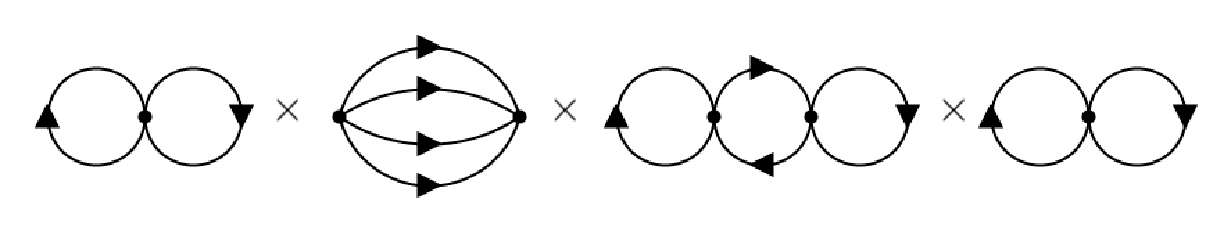
\includegraphics[width=0.60\textwidth, valign=c]{figurer/feynman-diagram/diagram_sum.pdf}
    \dots
\end{align}
%
If sub-diagram $i$ as a stand-alone diagram equals $\Em_i$, each copy of that subdiagram contributes a factor $\Em_i$ to the total diagram.
However, due to the symmetry of permuting identical subdiagrams, one must divide by the extra symmetry factor $s = n_i !$, the total number of permutations of all the copies of diagram $i$.
The full diagram therefore equals
%
\begin{align}
    \Em
    = \prod_{i= 1}^N \frac{1}{n_i!} \Em_i^{n_i}.
\end{align}
%
$\Em$ is uniquely defined by a finite sequence of integers, $(n_1, n_2, \dots n_N, 0, 0, \dots)$, so the sum of all diagrams is the sum over the set $S$ of all finite sequences of integers.
This allows us to write the sum of all diagrams as
%
\begin{equation}
    \label{sum of all diagrams}
    \sum_{(n_1, ...)\in S} \prod_{i} \frac{1}{n_i!} \Em_i^{n_i}
    = \prod_{i = 1}^{\infty} \sum_{n_i=1}^{\infty} \frac{1}{n_i!} \Em_i^{n_i}
    = \exp{{\sum}_i \Em_i}.
\end{equation}
%
We showed that the generating functional $Z[J]$ were the $Z_0[0]$ times the sum of all diagrams due to external sources.
From \autoref{sum of all diagrams}, if we define
%
\begin{equation}
    Z[J] = Z_0[0]\exp{i W[J]},
\end{equation}
%
then $W[J]$ is the sum of all connected diagrams. This is trivially true for the free theory, where the only connected diagram is
%
\begin{equation}
    \label{generating functional of connected diagrams}
    W_0[J] = J(x) \,\,
    \feynmandiagram [horizontal=a to b]{
        a [dot] -- [fermion] b [dot]
    };
    \,\,
    J(y).
\end{equation}
%
The two-point function in the full, interacting theory can thus be written
%
\begin{equation}
    -i \fdv{W[J]}{J(x),J(y)} = D(x - y).
\end{equation}


    \section{*The 1PI effective action}

\label{section: effective action}
This section is based on \autocite{peskinIntroductionQuantumField1995,schwartzQuantumFieldTheory2013,weinbergQuantumTheoryFields1995,weinbergQuantumTheoryFields1996}


The generating functional for connected diagrams, $W[J]$, is dependent on the external source current $J$.
We can define a new quantity with a different independent variable, using the Legendre transformation analogously to what is done in thermodynamics and Lagrangian mechanics.
The new independent variable is
\begin{equation}
    \varphi_J(x) := \frac{\delta W[J]}{\delta J(x)} = \ex{\varphi(x)}_J.
\end{equation}
%
The subscript $J$ on the expectation value indicate that it is evaluated in the presence of a source.
The Legendre transformation of $W$ is then
\begin{equation}
    \label{1PI effective action}
    \Gamma[\varphi_J]
    = W[J] - \int \dd^4 x \, J(x) \varphi_J(x).
\end{equation}
%
Using the definition of $\varphi_J$, we have that
\begin{equation}
    \label{effective equation of motion}
    \fdv{\Gamma[\varphi_J]}{\varphi_J(x)}
    = \int \dd^4 y \, \fdv{J(y)}{\varphi_J(x)} \fdv{J(y)} W[J]
    - \int \dd^4 y \, \fdv{J(y)}{\varphi_J(x)} \varphi_J(y)
    - J(x)
    = - J(x).
\end{equation}
%
If we compare this to the classical equations of motion of a field $\varphi$ with the action $S$,
\begin{equation}
    \frac{\delta S[\varphi]}{\delta \varphi(x)} = -J(x),
\end{equation}
%
we see that $\Gamma$ is an action that gives the equation of motion for the expectation value of the field, given a source current $J(x)$.

To interpret $\Gamma$ further, we observe what happens if we treat $\Gamma[\varphi]$ as a classical action with a coupling $g$.
The generating functional in this new theory is
\begin{equation}
    \label{partition function with g}
    Z[J, g] = \int \D \varphi \,
    \exp{ i g^{-1} \left( \Gamma[\varphi] + \int \dd^4x \, \varphi(x) J(x) \right) }
\end{equation}
%
The free propagator in this theory will be proportional to $g$, as it is given by the inverse of the equation of motion for the free theory.
All vertices in this theory, on the other hand, will be proportional to $g^{-1}$, as they are given by the higher-order terms in the action $g^{-1}\Gamma$.
This means that a diagram with $V$ vertices and $I$ internal lines is proportional to $g^{I-V}$.
Regardless of what the Feynman-diagrams in this theory are, the number of loops of a connected diagram is\footnote{This is a consequence of the Euler characteristic $\chi = V - E + F$.}
\begin{equation}
    \label{Number of loops}
    L = I - V + 1.
\end{equation}
%
To see this, we first observe that diagrams with one single loop must have equally many internal lines as vertices, so the formula holds for $L = 1$.
The formula still holds if we add a new loop to a diagram with $n$ loops by joining two vertices.
If we attach a new vertex with one line, the formula still holds, and as the diagram is connected, any more lines connecting the new vertex to the diagram will create additional loops.
This ensures that the formula holds by induction.
As a consequence of this, any diagram is proportional to $g^{L-1}$.
This means that in the limit $g \rightarrow 0$, the theory is fully described at the tree-level, i.e., by only considering diagrams without loops.
In this limit, we may use the stationary phase approximation, as described in \autoref{appendix: Functional derivatives}, which gives
\begin{equation}
    Z[J, g\rightarrow 0] \approx 
    C \det\left(- \fdv{ \Gamma[\varphi_J]}{\varphi(x), \varphi(y)}\right)\,
    \exp{i g^{-1} \left(\Gamma[\varphi_J] + \int \dd^4x \, J(x) \varphi_J(x) \right)  }.
\end{equation}
%
This means that
\begin{equation}
    -i g \ln(Z[J, g]) 
    = g W[J, g] 
    = \Gamma[\varphi_J] + \int \dd^4x\,  J(x) \varphi_J(x) + \mathcal{O}(g),
\end{equation}
%
which is exactly the Legendre transformation we started out with, modulo the factor $g$.
$\Gamma$ is, therefore, the action that describes the full theory at the tree level.
For a free theory, the classical action $S$ equals the effective action.

As we found in the last section, the propagator $D(x, y) = \ex{\varphi(x)\varphi(y)}_J$ is given by $-i$ times the second functional derivative of $W[J]$.
Using the chain rule, together with \autoref{effective equation of motion}, we get
%
\begin{align*}
    \label{Effective action inverse propagator}
    (-i)\int \dd^4 z \frac{\delta^2 W[J]}{\delta J(x) \delta J(z)} 
    \frac{\delta^2 \Gamma[\varphi_J]}{\delta \varphi_J(z) \varphi_J(y)}
    =
    (-i)\int \dd^4 z \frac{\delta \varphi_J[z]}{\delta J(x)}
    \frac{\delta^2 \Gamma[\varphi_J]}{\delta \varphi_J(z) \varphi_J(y)}
    =
    (-i)\fdv{}{J(x)}  \fdv{\Gamma[\varphi_J]}{\varphi_J(y)}
    = i\delta(x - y).
\end{align*}
%
This is exactly the definition of the inverse propagator,
%
\begin{equation}
    \fdv{\Gamma[\varphi_J]}{\varphi_J(x),\varphi_J(y)} = D^{-1}(x, y).
\end{equation}
%
The inverse propagator is the sum of all one-particle-irreducible (1PI) diagrams, with two external vertices.
More generally, $\Gamma$ is the generating functional for 1PI diagrams, which is why it is called the 1PI effective action.

$\Gamma$ may be viewed as an effective action as defined in the introduction.
We define $\eta$ as the fluctuations around the expectation value of the field, $\varphi(x) = \varphi_J(x) + \eta(x)$, and use this to change variables of integration in the path integral.
The expectation value $\varphi_J$ is constant with respect to the integral, so 
\begin{equation}
    \int \D \varphi \, \exp{i S[\varphi]}
    = \int \D \eta \, \exp{iS[\varphi_J + \eta]}.
\end{equation}
%
By assumption, $\ex{\eta}_J = 0$, which means this path integral is described by only 1PI diagrams, connected or not. We can therefore write
%
\begin{equation}
    \exp{i \Gamma[\varphi_J]} = \int \D \eta \, \exp{iS[\varphi_J + \eta]}.
\end{equation}
%
As we will discuss later, we interpret this form as \emph{integrating out} the $\eta$ degrees of freedom, leaving us with an effective description of the physics dependent only on the ground state solution $\varphi_J$.
The disadvantage of this is that there is no bound on how complicated $\Gamma$ might be---it is not restricted by the usual assumptions of the form of the action, such as locality~\autocite{schwartzQuantumFieldTheory2013}.
With some simplifying assumptions, though, we can still make use of the 1PI effective action, as we will see in the next subsection.




\subsection{Effective potential}

For a constant field configuration $\varphi(x) = \varphi_0$, the effective action, a functional, becomes a regular function.
We define the effective potential $\Veff$ by
%
\begin{equation}
    \label{definition effective potential}
    \Gamma[\varphi_0] = - V T \, \Ve_{\mathrm{eff}}(\varphi_0),
\end{equation}
%
where $VT$ is the volume of space-time.
For a constant ground state, the effective potential will equal the energy of this state.
To calculate the effective potential, we can expand the action around this state to calculate the effective action,
by changing variables to $\varphi(x) = \varphi_0 + \eta(x)$.
$\eta(x)$ now parametrizes fluctuations around the ground state, and has by assumption a vanishing expectation value.
The generating functional becomes
%
\begin{align}
    Z[J] 
    = \int \D (\varphi_0 + \eta) \, 
    \exp{i S[\varphi_0 + \eta] + i \int \dd^4 x\, [\varphi_0 + \eta(x)] J(x) }.
\end{align}

The functional version of a Taylor expansion, as described in \autoref{appendix: Functional derivatives}, is
%
\begin{equation}
    S[\varphi_0 + \eta] = 
    S[\varphi_0]
    + \int \dd x \, \eta(x) \, \fdv{S[\varphi_0]}{\varphi(x)}
    + \frac{1}{2} \int \dd x \dd y\,  \eta(x) \eta(y) \,
    \frac{\delta^2 S[\varphi_0]}{\delta\varphi(x)\delta\varphi(y)}
    + \dots
\end{equation}
%
The notation
%
\begin{equation}
    \fdv{S[\varphi_0]}{\varphi(x)}
\end{equation}
%
indicates that the functional $S[\varphi]$ is differentiated with respect to $\varphi(x)$, then evaluated at $\varphi(x) = \varphi_0$.
We define
%
\begin{align}
    S_0[\eta] &:= 
    \int \dd^4 x \dd^4 y \,\eta(x)\eta(y)\, 
    \fdv{S[\varphi_0]}{\varphi(x), \varphi(y)}, \\
    S_I[\eta] &:=
    \int \dd^4 x \dd^4 y \dd^4 z \,\eta(x)\eta(y)\eta(z)\, 
    \fdv{S[\varphi_0]}{\varphi(x),\varphi(y),\varphi(z)} + \dots,
\end{align}
%
where the dots indicate higher derivatives.
When we insert this expansion into the generating functional $Z[J]$ we get
%
\begin{align}
    &Z[J] = \int \D \eta \,
    \exp{
        i \int \dd^4 x \left(  \Ell[\varphi_0] + J \varphi_0  \right)
        +i \int \dd^4x \, \eta(x) \, 
        \left(  \fdv{S[\varphi_0]}{\varphi(x)} + J(x) \right)
        + i S_0[\eta] + i S_I[\eta]
    }.
\end{align}
%
The first term is constant with respect to $\eta$ and may be taken outside the path integral.
The second term gives rise to tadpole diagrams, which alter the expectation value of $\eta(x)$.
For $J=0$, this expectation value should vanish, and this term can be ignored.
Furthermore, this means that the ground state must minimize the classical potential,
\begin{equation}
    \label{minimize classical potential}
    \pdv{\Ve(\varphi_0)}{\varphi} = 0.
\end{equation}
%
%
This leaves us with 
%
\begin{equation}
    -i \ln Z[J] = W[J]
    =
    \int \dd^4 x \left(  \Ell[\varphi_0] + J \varphi_0  \right)
    -i \ln
    \left(
        \int \D \eta\exp{i S_0[\eta] + i S_I[\eta]}
    \right).
\end{equation}
%
%
We can now use the definition of the 1PI effective action to obtain a formula for the effective potential,
%
\begin{equation}
    \Veff(\varphi_0)
    =- \frac{1}{VT}
    \left( 
        W[J] - \int \dd^4 x \, J(x) \varphi_0
    \right)
    = \Ve(\varphi_0) 
    -i \ln
    \left(
        \int \D \eta\exp{i S_0[\eta] + i S_I[\eta]}
    \right).
\end{equation}
%

In \autoref{1PI effective action}, we showed that the 1PI effective action describes the whole quantum theory of the original action at the tree-level.
This was done by inspecting a theory with an action proportional to $g^{-1}$.
In this theory, Feynman diagrams with $L$ loops are proportional to $g^{L-1}$.
We can use the same argument to expand the effective potential in loops.
This is done by modifying the action $S[\varphi] \rightarrow g^{-1}S[\varphi]$, and then expand in power of $g$.
The first term in the effective potential is modified by $\Ve \rightarrow g^{-1}\Ve$, which means that it is made up of tree-level terms.
This is as expected, since the tree-level result corresponds to the classical result without any quantum corrections.
The second term becomes
%
\begin{align*}
    \ln
    \left(
        \int \D \eta \, e^{i S_0 + i S_I}
    \right)
    \longrightarrow
    &
    \ln
    \left(
        \int \D \eta \, e^{i g^{-1}S_0 + i g^{-1} S_I}
    \right)
    = 
    \ln\left(
        \int \D \eta \, e^{i g^{-1}S_0}
    \right)
    +
    \ln
    \left(
        \frac{
            \int \D \eta\, e^{i g^{-1} S_I} \, e^{i g^{-1}S_0}
        }{
            \int \D \eta\,e^{i g^{-1}S_0}
        }
    \right)
\end{align*}
%
The first term is quadratic in $\eta$, and can therefore be evaluated as a generalized Gaussian integral, as described in \autoref{appendix: Functional derivatives},
%
\begin{align*}
    & 
    \ln\Bigg[
        \int \D \eta \, 
    \exp{
            i g^{-1} \frac{1}{2} \int \dd^4x \dd^4y\,  \eta(x) \eta(y) \, 
            \fdv{S[\varphi_0]}{\varphi(x),\varphi(y)} 
    }
    \Bigg]
    \\
    & 
    = 
    \ln\Bigg[
        \det\left( - g^{-1} \fdv{S[\varphi_0]}{\varphi(x), \varphi(y)} \right)^{-1/2}
    \Bigg]
    = -\frac{1}{2}
    \Tr{
        \ln\left[
        - \fdv{S[\varphi_0]}{\varphi(x), \varphi(y)}
        \right]
    }
    + \const
\end{align*}
%
We then use the identity $\ln\{\det M \}= \Tr{\ln M}$.
After we remove the constant, this term is proportional to $g^0$, i.e., it is made up of one-loop terms.

The last term can be evaluated by first expanding the exponential containing the $S_I$ term, then using $\ln(1 + x) = \sum_n \frac{1}{n}x^n$.
Using
%
\begin{equation}
    \ex{A}_0 =  \frac{
        \int \D \varphi \, 
        A \, e^{ig^{-1}S_0}
    }{
        \int \D \varphi \, 
        e^{ig^{-1}S_0}
    },
\end{equation}
%
we can write
%
\begin{align}
    & \ln
    \left[
        \frac{
            \int \D \eta \, 
            e^{ig^{-1}S_I}e^{ig^{-1}S_0}
        }{
            \int \D \varphi \, 
            e^{ig^{-1}S_0}
        }
    \right]
    = 
    \ln 
    \left(
        \sum_{n = 0}^\infty \frac{1}{n!}
        \ex{(ig^{-1}S_I)^n}_0
    \right).
\end{align}
%
We recognize this as the sum of all connected Feynman diagrams, with Feynman rules from the interaction term $S_I$.
We know that $S_I$ is made up of terms that are third power or higher in the fields.
Each internal line is connected to two vertices, and each vertex is connected to at least three internal lines, i.e., $I \geq 3/2 V$.
The number of loops is therefore $L = I - V + 1 \geq (3/2 - 1)V + 1$.
There is at leas one vertex, i.e. $L \geq 3/2$.
This shows that the first logarithm contains \emph{all} one-loop contributions.
The effective potential to one-loop order is therefore
%
\begin{equation}
    \label{effective potential}
    \Veff(\varphi_0) = \Ve(\varphi_0) - \frac{i}{VT}  \frac{1}{2} \Tr{\ln\left( - \fdv{S[\varphi_0]}{\varphi(x), \varphi(y)}  \right)}.
\end{equation}
%


    \section{Symmetry and Goldstone's theorem*}
\label{section:symmetry}

This section is based on~\autocite{leeIntroductionSmoothManifolds2003d,peskinIntroductionQuantumField1995,schwartzQuantumFieldTheory2013,weinbergQuantumTheoryFields1995,weinbergQuantumTheoryFields1996}.

Symmetry plays a prominent role in modern physics.
If we can transform a physical state in such a way that the governing equations of this system are unchanged, we call that transformation a \emph{symmetry transformation}.
All such transformations are known as the symmetries of that theory.
The symmetries of a theory encode a lot of physics, such as the presence of conserved quantities and the system's low energy behavior.
We distinguish between internal and external symmetries.
An external symmetry is an active coordinate transformation, such as rotations or translations.
They relate degrees of freedom at different space-time points, while internal symmetries transform degrees of freedom at each space-time point independently.
A further distinction is between global and local symmetry transformations.
Global transformations have one rule for transforming degrees of freedom at each point, which is applied everywhere, while local transformations are functions of space-time.

In classical field theory, symmetries are encoded in the behavior of the Lagrangian when the fields are transformed.
We will consider continuous transformations, which can in general be written as
\begin{equation}
    \varphi(x) \longrightarrow \varphi'(x) = f_t[\varphi](x), \quad t \in [0, 1].
\end{equation}
%
Here, $f_t[\varphi]$ is a functional in $\varphi$, and a smooth function of $t$, with the constraint that $f_0[\varphi] = \varphi$.
This allows us to look at ``infinitesimal'' transformations,
\begin{equation}
    \label{infinitesimal transformation}
    \varphi'(x) = f_\epsilon[\varphi] 
    = \varphi(x) + \epsilon \odv{ f_t[\varphi] }{t}\bigg |_{t=0} + \Oh{\epsilon}.
\end{equation}
%
When considering infinitesimal transformations, we will not always write $ + \Oh{\epsilon}$, but rather consider it implicit.
We will consider internal, global transformations which act linearly on $\varphi$.
For $N$ fields, $\varphi_i$, this can be written
\begin{equation}
    \label{linear field transformation}
    \varphi_i'(x) = \varphi_i(x) + \epsilon \, i V_{ij} \varphi_j(x).
\end{equation}
%
$V_{ij}$ is called the generator of the transformation.
A symmetry transformation of the system is then a transformation in which the Lagrangian left is unchanged, or at most differ by a 4-divergence term.
That is, a transformation $\varphi \rightarrow \varphi'$ is a symmetry if 
\begin{equation}
    \Ell[\varphi'] = \Ell[\varphi] + \partial_\mu K^\mu[\varphi],
\end{equation}
%
where $K^\mu[\varphi]$ is a functional of $\varphi$.\footnote{Terms of the form $\partial_\mu K^\mu$ does not affect the physics, as variational principle $\delta S = 0$ do not vary the fields at infinity. Together with the divergence theorem, this means that such terms do not influence the equations of motion.}
This is a requirement for symmetry in quantum field theory too.
However, as physical quantities in quantum field theory are given not just by the action of a single state but the path integral, the integration measure $\D \varphi$ has to be invariant as well.
If a classical symmetry fails due to the non-invariance of the integration measure, it is called an \emph{anomaly}.

To investigate the symmetry properties of a quantum theory, we explore what constraints a symmetry imposes on the effective action.
To that end, assume 
\begin{equation}
    \D \varphi'(x) = \D \varphi(x), \quad
    S[\varphi'] = S[\varphi].
\end{equation}
%
In the generating functional, such a transformation corresponds to a change of integration variable.
Using the infinitesimal version of the transformation, we may write
\begin{align}
    \nonumber
    Z[J]
    = \int \D \varphi \, \exp{i S[\varphi] + i \int \dd^4 x \,J_i(x) \varphi_i(x)} 
    = \int \D \varphi' \, \exp{i S[\varphi'] + i \int \dd^4 x \, J_i(x) \varphi'_i(x)}
    \\
    = Z[J] + i \epsilon \int \dd^4 x \, J_i(x) \int \D \varphi \, [V_{ij} \varphi_j(x)]  e^{i S[\varphi]},
\end{align}
%
Using \autoref{effective equation of motion}, we can write this as
\begin{equation}
    \label{effective action symmetry requirement}
    \int \dd^4 x \, \fdv{\Gamma[\varphi_J]}{\varphi_i(x)} \, V_{ij}\ex{\varphi_j(x)}_J = 0.
\end{equation}
%
This constraint will allow us to deduce the properties of a theory close to the ground state, only using information about the symmetries of the theory.


The archetypical example of an internal, global, and continuous symmetry is the linear sigma model, which we will use as an example throughout this section.
The linear sigma model is made up of $N$ real scalar fields $\varphi_i$, whose Lagrangian is
\begin{equation}
    \Ell[\varphi] 
    = \frac{1}{2} \partial_\mu \varphi_i(x) \partial^\mu \varphi_i(x) - \Ve(\varphi),
    \quad \Ve(\varphi) = - \frac{1}{2} \mu^2 \varphi_i(x)\varphi_i(x)
    + \frac{1}{4} \lambda [\varphi_i(x) \varphi_i(x)]^2.
\end{equation}
%
This system is invariant under the rotation of the $N$ fields into each other,
\begin{equation}
    \varphi_i \longrightarrow \varphi_i' = M_{ij} \varphi_j,
    \quad M^{-1} = M^{T}.
\end{equation}
%
The set of all such transformations forms the Lie group $\text{O}(N)$.
Lie groups will be discussed in the next section.
For $N = 2$, and $\mu^2, \lambda > 0$ we get the ubiquitous Mexican hat potential, as illustrated in \autoref{fig:Mexican hat}.

\begin{figure}[ht]
    \centering
    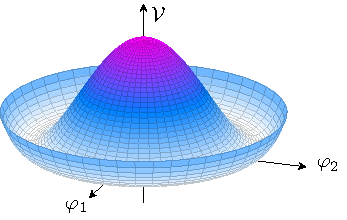
\includegraphics[width=0.6\textwidth]{figurer/mexican_hat.pdf}
    \caption{The Mexican hat potential is the classical potential $\Ve$ for the $N=2 $ linear sigma model.}
    \label{fig:Mexican hat}
\end{figure}

\subsection{Nöther's theorem}

One of the most profound consequences of symmetry in physics is the appearance of conserved quantities.
Assume we have a set of fields $\varphi_i$. Nöther's theorem tells us that if the Lagrangian $\Ell[\varphi_i]$ has a continuous symmetry, then there is a corresponding conserved current~\autocite{carrollSpacetimeGeometryIntroduction2019,peskinIntroductionQuantumField1995}.
Consider an infinitesimal transformation,
\begin{equation}
    \varphi_i(x) \longrightarrow \varphi_i'(x)
    = \varphi_i(x) + \delta \varphi_i(x),.
\end{equation}
%
Applying this transformation to the Lagrangian will in general change its form,
\begin{equation}
    \Ell[\varphi] \rightarrow \Ell[\varphi']
    = \Ell[\varphi] + \delta \Ell.
\end{equation}
%
We assume this transformation is a symmetry, i.e.,
\begin{equation*}
    \delta \Ell = \partial_\mu K^\mu.
\end{equation*}
%
By considering the Lagrangian as a function of the field and its derivatives, $\Ell = \Ell(\varphi_i, \partial_\mu \varphi_i)$, we can write the difference term as a Taylor expansion around $(\varphi_i, \partial_\mu \varphi_i)$,
\begin{align}
    \delta \Ell
    = \pdv{\Ell}{\varphi_i} \delta \varphi_i
    + \pdv{\Ell}{(\partial_\mu \varphi_i)} \delta (\partial_\mu \varphi_i),
\end{align}
%
where $\delta (\partial_\mu \varphi_i) = \partial_\mu \varphi_i' - \partial_\mu \varphi_i$.
By the linearlity of the derivative,
\begin{equation}
    \delta (\partial_\mu \varphi_i)
    = \partial_\mu \varphi_i' - \partial_\mu \varphi_i
    = \partial_\mu (\varphi_i' - \varphi_i)
    = \partial_\mu \delta \varphi_i.
\end{equation}
%
With this, and the Euler-Lagrange equations
\begin{equation}
    \partial_\mu \pdv{\Ell}{(\partial_\mu \varphi)} - \pdv{\Ell}{\varphi_i} = 0,
\end{equation}
%
we can rewrite
\begin{equation}
    \delta \Ell = \left( \partial_\mu \pdv{\Ell}{(\partial_\mu \varphi_i)} \right) \delta \varphi_i
    + \pdv{\Ell}{(\partial_\mu \varphi_i)} (\partial_\mu \delta \varphi_i)
    = \partial_\mu \left(\pdv{\Ell}{(\partial_\mu \varphi_i)} \delta \varphi_i\right)
\end{equation}
%
If we define the current
\begin{equation}
    j^\mu = \pdv{\Ell}{(\partial_\mu \varphi_i)} \delta \varphi_i(x) - K^\mu,
\end{equation}
%
then 
\begin{equation}
    \partial_\mu j^\mu = \delta \Ell - \delta \Ell = 0.
\end{equation}
%
This is Nöther's theorem; a continuous symmetry implies the existence of a conserved current.

The current flux through some spacelike surface $V$ defines a conserved charge. The surface of constant time in some reference frame has the normal vector $n_\mu = (1, 0, 0, 0)$, so the charge is
\begin{equation}
    Q = \int_V \dd^4 x \, n_\mu j^\nu = \int_V \dd^3 x \, j^0.
\end{equation}
%
We can then use the divergence theorem.
Assume $\partial V$ is the boundary of $V$, which has the space-like normal vector $k_i$, and that the current falls of quickly towards infinity.
Then
\begin{equation}
    \odv{Q}{t} = - \int_V \dd^3 x \, \partial_i j^i = - \int_{\partial V} \dd^2 x\, k_i j^i = 0,
\end{equation}
%
proving that the charge is conserved.

\subsection{Goldstone's theorem}

A symmetry transformation will leave the governing equation of a theory unchanged.
This, however, does not imply that physical states, such as the ground state, are invariant under this transformation.
The $N = 2$ linear sigma model illustrates this.
If we assume the ground state $\varphi_{0}$ is translationally invariant, then it is given by minimizing the effective potential, of which the classical potential, $\Ve$, is the leading order approximation.
This potential is illustrated in \autoref{fig:Mexican hat}.
The ground state is therefore given by any of the values along the brim of the potential.
If we, without loss of generality, choose $\varphi_0 = (0, v)$ as the ground state, then any rotation will change this state.
We say that the symmetry has been \emph{spontaneously broken}.

To explore this in a general context, assume a theory of $N$ real scalar fields $\varphi_i$ are invariant under the actions of some Lie group, $G$.
A symmetry $g \in G$ is broken if the vacuum expectation value of the original fields and the transformed fields differ.
That is, if
\begin{equation}
    \ex{\varphi}_0 \neq \ex{\varphi'}_0 = \ex{g \varphi}_0
\end{equation}
%
We can now exploit what we learned about Lie groups to write the infinitesimal transformation as
\begin{equation}
    \ex{\varphi'}_0 = \ex{\varphi}_0 + i \epsilon \eta_\alpha T_\alpha \ex{\varphi}_0.
\end{equation}
%
Let $x_i$ be the set of generators corresponding to broken symmetries, i.e.,
\begin{equation}
    x_i \ex{\varphi}_0 \neq 0.
\end{equation}
%
These are called the \emph{broken generators}.
The remaining set of generators $t_a$, which obey
\begin{equation}
    t_a \ex{\varphi}_0 = 0,
\end{equation}
%
are called unbroken, and generate a subgroup $H \subset G$ as the set of symmetry transformations of the vacuum is a group.

In \autoref{effective action symmetry requirement} we found that, if $V$ is the generator of some symmetry, then the effective action obeys
\begin{equation}
    \int \dd^4 x\, \fdv{\Gamma[\varphi_J]}{\varphi_i} V_{ij} \ex{\varphi_j}_0 = 0,
\end{equation}
%
We now differentiate this expression with respect to $\varphi_k(y)$ and evaluate it in the vacuum, which gives
\begin{equation}
    \int \dd^4 x \, \fdv{\Gamma[\varphi_0]}{\varphi_k(y), \varphi_i(x)}
    V_{ij} \ex{\varphi_j}_0 = 0.
\end{equation}
%
With the assumption that the ground state is constant, we get 
\begin{equation}
    \pdv{\Veff}{\varphi_k, \varphi_i} \, V_{i j} \ex{\varphi_j}_0 = 0.
\end{equation}
%
This is trival for unbroken symmetries, as $t^a_{ij}\ex{\varphi_j}_0 = 0$ by definition.
However, in the case of a broken symmetry, the second derivative of the effective potential has an eigenvector $x^\ell_{ij} \ex{\varphi_j}_0$ with a zero eigenvalue for each broken generator.
Here, $\ell$ label the set of generators, while $(ij)$ are the indices corresponding to field-components $\varphi_i$.
In \autoref{Effective action inverse propagator}, we found that the second derivative of the effective action is the inverse propagator,
\begin{equation}
    D^{-1}_{ij}(x,y) 
    = \fdv{\Gamma[\varphi_0]}{\varphi_i(y), \varphi_j(x)}
    = \int \frac{\dd^4 p}{(2 \pi)^4} e^{-ip(x - y)} \, \tilde D^{-1}_{ij}(p).
\end{equation}
%
Using this, we can write
\begin{equation}
    \tilde D^{-1}_{i j}(p=0) \, x^\ell_{jk} \ex{\varphi_k}_0 
    = 0.
\end{equation}
%
Zeros of the inverse propagator correspond to the physical mass of particles.
In Lorentz-invariant systems, each zero-eigenvalue vector corresponds to a masses particle, called a Goldstone boson.\footnote{ The particles are bosons due to the bosonic nature of the transformations, $g$. If the generators are Grassmann numbers, the resulting particles, called goldstinos, are fermions.}
This means there are $n_G = \dim G -\dim H$ zero-mass modes.
In general, the counting of massless modes is complicated and depends on the dispersion relation of the particles at low momenta.
Systems with Goldstone bosons with quadratic dispersion relation, that is $E \propto |\vv p|^2$ when $\vv p \rightarrow 0$, often exhibit a lower number of massless modes.
An example is ferromagnets, where the $\mathrm{SU}(2)$ rotational symmetry is broken down to $\mathrm{U}(1)$ when they align along one axis. 
This corresponds to two broken generators, yet the system exhibits only one massless mode~\autocite{braunerSpontaneousSymmetryBreaking2010}.

\begin{figure}[ht]
    \centering
    \hspace*{2.5cm}
    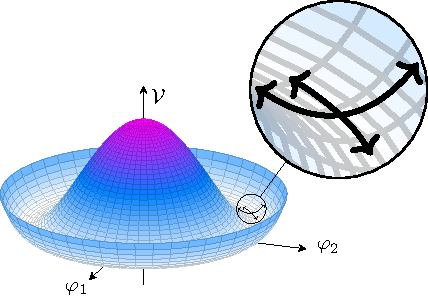
\includegraphics[width=.6\linewidth]{figurer/mexican_hat_zoom.pdf}
    \caption{Excitations along the brim does not cost any energy, as the potential is flat, unlike excitations in the radial direction.}
    \label{fig:Mexican hat zoom}
\end{figure}

The linear sigma model gives an intuition for the Goldstone mode.
In the case of $N = 2$, the symmetry of the Lagrangian are rotations in the plane.
As the ground state is a point along the ``brim'' of the hat, this rotational symmetry is broken.
However, any excitations in the angular direction do not cost any energy, which is indicative of a massless mode.
This is illustrated in \autoref{fig:Mexican hat zoom}.
In this example, the original symmetry group is one-dimensional, so there are no unbroken symmetries.
Consider instead the $N=3$ linear sigma model, which has the three-dimensional symmetry group $\SO(3)$, rotations of the sphere.
We see that the ground state is left invariant under a subgroup of the original symmetry transformations.
The ground state manifold of this system, the set of all states that minimizes the effective potential, is then a sphere.
When the system chooses one single ground state, this symmetry is broken, but only for two of the generators. 
The generator for rotations around the ground state leaves that point unchanged and is thus an unbroken symmetry.
Any excitations in the direction of the broken symmetries do not cost energy, as it is in the ground state manifold.
On the other hand, the unbroken symmetry does not correspond to an excitation.
This is illustrated in \autoref{fig:ground state manifold}.

\begin{figure}[h]
    \centering
    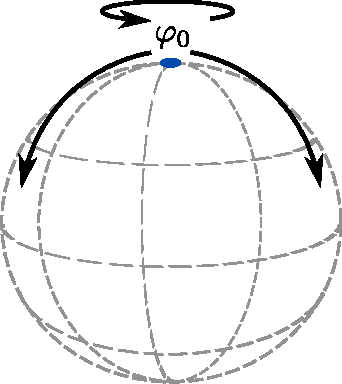
\includegraphics[width=.35\linewidth]{figurer/SU(3).pdf}
    \caption{Excitations for the $N=3$ sigma model. Two of the symmetries are broken, while rotations around the groundstate leaves the system unchanged.}
    \label{fig:ground state manifold}
\end{figure}

    \section{CCWZ construction*}
\label{seciton:ccwz construction}

As Goldstone bosons are massless, they play a crucial role in low-energy dynamics.
To best describe this limit, we seek a parametrization of the theory in which they are the degrees of freedom.
This can be done using the CCWZ construction, named after Callan, Coleman, Wess, and Zumino.
This section is based on~\autocite{morrisonColemanCallanWessZuminoConstruction2017,panicoCompositeNambuGoldstoneHiggs2016,weinbergQuantumTheoryFields1996,pichEffectiveFieldTheory2020}, as well as the original papers~\autocite{callanStructurePhenomenologicalLagrangians1969,colemanStructurePhenomenologicalLagrangians1969}.


We saw that the Goldstone bosons correspond to excitations within the vacuum manifold.
The vacuum manifold corresponds to points in field space $\varphi$ that can be reached from the vacuum $\varphi_0$ with a transformation $g \in G$.
Assume this group acts linearly on the fields.
This means that we can write such excitations as
\begin{equation}
    \varphi_i = (\tilde\Sigma \varphi_0)_{i} = \tilde \Sigma_{ij} (\varphi_0)_j, 
    \quad \tilde \Sigma = \tilde \Sigma(\eta) = \exp{i \eta_\alpha T_\alpha}
\end{equation}
%
We will drop the indices for the sake of compact notation.
$\tilde \Sigma$ is thus a function from the parameter space, $\eta_\alpha \in \R^n$, to $G$,
\begin{align}
    \tilde \Sigma: \R^n \longmapsto G.
\end{align}
%
We then get space-time-dependent field configurations by making the parameters dependent on space-time.
We will for now assume $\eta_\alpha$ is constant.
This parametrization is highly redundant.
Two elements $\tilde\Sigma$ and $\tilde\Sigma'$, related by
\begin{equation}
    \tilde \Sigma' = \tilde\Sigma e^{i \theta_a t_a}
\end{equation}
%
results in the same $\varphi$.
This is because  $e^{i \theta_a t_a} = h \in H$, and $h \varphi_0 = \varphi_0$, by assumption.
The set of all equivalent $\tilde \Sigma$'s is exactly the left coset, $gH = \setbuilder{gh}{ h \in H}$.
The set of cosets forms a new manifold, $G / H$, called the Goldstone manifold.
This is a manifold of dimension $\dim(G/H) = \dim(G) - \dim(H)$, which is the number of broken generators and thus also the number of Goldstone modes.
Membership of a certain coset form an equivalence relation, $g \sim g'$ if $g' = gh$.
This means that the cosets $gH$ form a partition of $G$ and that each element $g \in G$ belongs to one, and only one, coset.
To remove the redundancy in the parametrization, we need to choose one representative element from each coset.

By the inverse function theorem, any mapping between manifolds $f: \Em \mapsto \mathcal{N}$ that has a non-degenerate differential, that is an invertible Jacobian, at a point $p \in \Em$, is invertible in a neighborhood of $p$.
If we write
\begin{equation}
    \tilde \Sigma(\xi, \theta) = \exp{i \xi_i x_i} \exp{i \theta_a t_a},
\end{equation}
%
then the map is invertible at $p = (\xi_i = 0, \theta_a = 0)$, as the Jacobian is the identity matrix.
This point is mapped to the identity element of $G$.
This means that, in a neighborhood $U \subset G$ of the identity, each element $g$ has a unique representation $g = \tilde \Sigma$~\autocite{leeSmoothManifolds2012}.
Furthermore, two elements $\tilde \Sigma'$ and $\tilde \Sigma$ related by $\tilde \Sigma' = \tilde \Sigma h$, $h \in H$ have the same $\xi$-arguments.
We see that $\xi_i$ parametrize $G/H$, in the neighborhood of the identity.
We therefore demand that $\tilde \Sigma$ always appear in the standard form
\begin{equation}
    \Sigma(\xi) = \tilde \Sigma(\xi, 0) = \exp{i \xi_i x_i}.
\end{equation}
%
The field $\varphi(x)$ can therefore be written as
\begin{equation}
    \varphi(x) = \Sigma(x) \varphi_0 = \exp{i \xi_i(x) x_i} \varphi_0,
\end{equation}
%
and $\xi_i(x)$ can be associated with the Goldstone bosons.

In the linear sigma model, the original $\Olie(N)$ symmetry is broken down to $\Olie(N-1)$, which transforms the remaining $N-1$ fields with vanishing expectation values into each other.
However, $\Olie(N)$ consists of two disconnected subsets, those matrices with determinant 1 and those with determinant -1.
There is no continuous path that takes an element of $\Olie(N)$ with determinant of $-1$ to an element with determinant 1.\footnote{A simple proof of this is the fact that the determinant is a continuous function, while any path $\det M(t)$ such that $\det M(1) = -1,\, \det M(0) = 1$ must make a discontinuous jump.}
The set of symmetries that are connected to the identity is
\begin{eqnarray}
    G = SO(N) = \setbuilder{M \in \Olie(N)}{ \det M = 1}.
\end{eqnarray}
If we choose $\varphi_0 = (0, 0, ..., v)$, then it is apparent that the ground state is invariant under the rotations of the $N-1$ first fields, so the unbroken symmetry is  $H = \SO(N-1)$.
The Goldstone manifold is $G/H = \SO(N) / \SO(N-1)$.

Consider the case of $N = 3$, which is illustrated in \autoref{fig:ground state manifold}.
$G$ is the rotations of the sphere, while $H$ is rotations around $\varphi_0$, $\SO(2)$.
The Goldstone manifold consists of the rotations of $\varphi_0$ to other points of the sphere, i.e. $G/H = \SO(3)/\SO(2) = S^2$, the 2-sphere.
This is not a Lie group, as translating $\varphi$ in a closed path around the sphere may result in a rotation around the z-axis.
This is illustrated in \autoref{fig:Curvature of SO(3)}


To check that $\xi_i$, in fact, are the Goldstone modes, we study the way they appear in the Lagrangian.
As they are massless, no mass term of the form $M_{ij} \xi_i \xi_j$ should appear.
The original Lagrangian $\Ell[\varphi]$ was invariant under global transformations $\varphi(x) \mapsto g \varphi(x)$.
However, any terms that only depend on $\varphi(x)$, and not its derivatives, will also be invariant under a \emph{local} transformation, $\varphi(x) \mapsto g(x)\varphi(x)$.
Our parametrization of the fields, $\varphi(x) = \Sigma(x)\varphi_0$ is exactly such a transformation, which means that any such terms are independent of the Goldstone bosons.
We can therefore write
\begin{equation}
    \Ell[\varphi] = \Ell_{\mathrm{kin}}[\varphi] + V(\varphi_0),
\end{equation}
%
where all terms in $\Ell_{\mathrm{kin}}$ are proportional to at least one derivative term, $\partial_\mu \varphi(x)$.
Inserting the parametrization into this derivative term, we get
\begin{equation}
    \partial_\mu \varphi(x) = \partial_\mu [\Sigma(x) \varphi_0]
    = \Sigma(x) [\Sigma(x)^{-1} \partial_{\mu} \Sigma(x)] \varphi_0.
\end{equation}
%
The Lagrangian will therefore depend on $\xi_i$ via terms of the form $\Sigma(x)^{-1}\partial_\mu \Sigma(x)$, which is called the Mauer-Cartan form.
This is a $\mathfrak g$-valued function, which means that it can be written as
\begin{align}
    i\Sigma(x)^{-1}\partial_\mu \Sigma(x) & 
    = d_{\mu}(x) + e_{\mu}(x), \\
    d_{\mu} & = i x_i d_{ij}(\xi) \partial_\mu \xi_j, \\
    e_{\mu} & = i t_a e_{ai}(\xi)\partial_\mu \xi_i,
\end{align}
%
where $d_{ij}$ and $e_{ai}$ are as-of-yet unknown real valued functions of $\xi$~\autocite{watanabeEffectiveLagrangianNonrelativistic2014,weinbergQuantumTheoryFields1996}.

\subsection{Transformation properties of Goldstone bosons}
We can deduce how the Goldstone bosons transforms under $G$ from how $\varphi$ transforms.
In general, 
\begin{equation}
    \varphi' = g \varphi = (g \Sigma(\xi)) \varphi_0 = \Sigma(\xi') \varphi_0 \quad g \in G.
\end{equation}
%
While $\Sigma(\xi')$ has the standard form by assumption,
\begin{equation}
    \Sigma(\xi') = \exp{i \xi'_i x_i},
\end{equation}
%
$g\Sigma(\xi)$ does not, in general.

\begin{figure}[h]
    \centering
    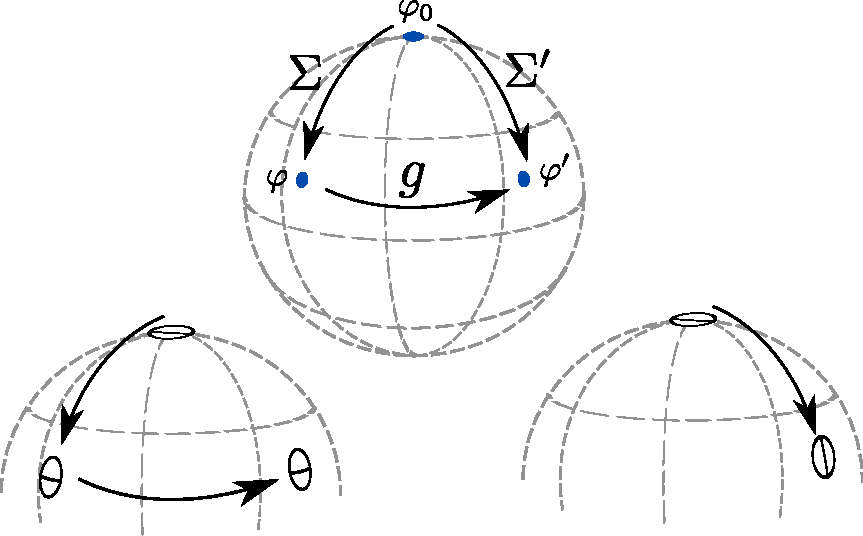
\includegraphics[width=0.8\textwidth]{figurer/curvature.pdf}
    \caption{The top figure illustrates the transformation of $\varphi_0$ to $\varphi$ and then $\varphi'$, and the alternative, direct transformation $\varphi_0 \rightarrow \varphi'$. The bottom figure illustrates how this can rotate a neighborhood of $\varphi_0$ differently.}
    \label{fig:Curvature of SO(3)}
\end{figure}
\autoref{fig:Curvature of SO(3)} illustrates this in the case of $G = \SO(3)$.
$\Sigma(\xi)$ transforms $\varphi_0$ to $\varphi$, then $g$ transforms $\varphi$ to $\varphi' = \Sigma(\xi') \varphi_0$.
Assuming $\varphi$ and $\varphi'$ are close enough to $\varphi_0$, we can write $\Sigma(\xi)$ and $\Sigma(\xi')$ on the standard form.
However, if we follow a small neighborhood around $\varphi_0$ as it is acted on by $\Sigma(\xi)$, then $g$, it will be rotated by the time it arrives at $\varphi'$ when compared to the same neighborhood if it was acted on by $\Sigma(\xi')$.

$g\Sigma(\xi)$ and $\Sigma(\xi')$ are in the same coset, as they by assumption corresponds to the same physical state.
This means that we can write $g\Sigma(\xi) = \Sigma(\xi') h(g, \xi)$, where $h(g, \xi) \in H$.
The transformation rule of $\xi$ under $G$ is therefore implicitly defined by
\begin{equation}
    \Sigma(\xi') = g \Sigma(\xi) [h(g, \xi)]^{-1}.
\end{equation}
%
This is, in general, not a linear representation, which is why this construction also is called a \emph{non-linear realization}.
Using the transformation rule, we can obtain the transformation rule of the Maurer-Cartan form.
We use the shorthand $\Sigma = \Sigma(\xi),\, \Sigma' = \Sigma(\xi')$, and $h = h(g, \xi)$.
This gives
\begin{align*}
    \Sigma^{-1} \partial_\mu \Sigma
    \rightarrow 
    & \, \Sigma'^{-1} \partial_\mu \Sigma' \\
    & = (g \Sigma h^{-1})^{-1} \partial_\mu (g \Sigma h^{-1}) \\
    & = (h \Sigma^{-1} g^{-1}) g [(\partial_\mu \Sigma)h^{-1} + \Sigma \partial_\mu h^{-1}] \\
    & = h \Sigma^{-1} (\partial_\mu \Sigma) h^{-1}
    + h \partial_\mu h^{-1} \\
    & = h (\Sigma^{-1} \partial_\mu \Sigma + \partial_\mu) h^{-1}.
\end{align*}
In terms of $d_\mu$ and $e_\mu$,
\begin{align}
    d_\mu & \rightarrow h d_\mu h^{-1} \\
    e_\mu & \rightarrow h (e_\mu + i\partial_\mu )h^{-1}.
\end{align}
%
These are our building blocks for constructing a general, $G$-invariant effective Lagrangian.
The trace of a product of $d_\mu$'s are invariant under $G$,
\begin{equation}
    \Tr{d_\mu d_\nu \dots d_\rho} 
    \rightarrow
    \Tr{h d_\mu h^{-1} h d_\nu h^{-1} h \dots d_\rho h^{-1}}
    = \Tr{d_\mu d_\nu \dots d_\rho},
\end{equation}
%
where we have used the cyclic property of trace.
However, the terms must also obey the other symmetries of the Lagrangian, such as C or P-parity and Lorentz invariance.
The last criterion excludes any terms with free space-time indices.
In \todo{Legg til dette}{section:chiral pertubation theory}, we will construct an effective Lagrangian in powers of $d$.
The lowest order terms are therefore
\begin{equation}
    \label{first order terms CCWZ}
    \Tr{d_\mu} \Tr{d^\mu}, 
    \quad 
    \Tr{d_\mu d^\mu}.
\end{equation}
%
We see that $e_\mu$ transforms like a gauge field, with the gauge group $H$.
If we include massive degrees of freedom and not only the Goldtone modes, $e_\mu$ is used to create a covariant derivative of the massive modes.
We are only interested in the Goldstone modes and will therefore be satisfied with $d_\mu$.
With these tools, we can create an effective theory of quantum chromodynamics at low energies.



    \chapter{General relativity and the TOV equation}
    \label{chapter: GR}
    (Newtonian gravity??)
\todo{Short about newtonian gravity/motivation}

\section{General relativity}
This section is based on~\cite{carrollSpacetimeGeometryIntroduction2019}.
The derivation of the spherically symmetric metric is done using computer code, as descirbed in \autoref{appendix: code}.

\subsection{Einstein's field equations}

General relativity describes spacetime as a smooth manifold $\Em$, with a (pseudo-Riemannian) metric, $g_{\mu \nu}$.
This metric is treated as a dynamical field, which is affected by the presence of matter and energy.
The matter and energy contents of spacetime are encoded in the stress-energy tensor $T_{\mu \nu}$, while the behavior of $g^{\mu \nu}$ is encoded in a scalar Lagrangian density.
Some of the mathematics used in this section, such as functional derivatives, are covered in \autoref{appendix: Functional derivatives}.

The most obvious---and correct---choice as the Lagrangian for $g^{\mu \nu}$ is the Ricci scalar, which results in the Einstein-Hilbert action,
%
\begin{equation}
    \label{Einstein-Hilbert action}
    S_{\text{EH}} = \frac{1}{2\kappa}\int_{\Em} \dd^n x \, \sqrt{|g|}\, R.
\end{equation}
%
The $\sqrt{|g|}$-factor is included for the integral to be coordinate-independent, as discussed in  \autoref{subsection: integration on manifolds}.\footnote{The gravitational action can also include a cosmological constant, modifying the Lagrangian to $R + 2 \Lambda$. This constant does not affect the subject of this thesis and is therefore not included here.}
The $\kappa$ is a constant and decides how strong the coupling of gravity to matter and energy is.
This constant can then be related to Newton's constant of gravitation $G$ by $\kappa = 8 \pi G$.
When including the contributions from other fields with an action $S_\text{m}$, the total action becomes 
%
\begin{equation}
    S = S_\text{EH} + S_\text{m}.
\end{equation}
%
The equations of motion of the dynamical field, which in this case is the metric, are given by Hamilton's principle of stationary action.
Using functional derivatives, as defined in \autoref{subsection: functional calculus on a curved manifold}, this is stated as
%
\begin{equation}
    \fdv{S}{g^{\mu\nu}} = 0,
\end{equation}
%
We define the stress-energy tensor as
%
\begin{equation}
    \label{definition stress energy densor}
    T_{\mu\nu} = - \frac{2}{\sqrt{|g|}} \fdv{S_\text{m}}{g^{\mu \nu}}.
\end{equation}
%
The functional derivative of the Einstein-Hilbert action is evaluated in \autoref{subsection: functional derivative of the einstein-hilbert action}, and with the result, \autoref{functional derivatie einstein-hilber action}, we get the Einstein field equations
%
\begin{equation}
    \label{Einstein field equations}
    R_{\mu \nu} - \frac{1}{2} R g_{\mu \nu} = \kappa T_{\mu \nu},
\end{equation}
%
The left-hand side of the Einstein field equations is called the Einstein tensor, $G_{\mu \nu} = R_{\mu \nu} - \frac{1}{2} R g_{\mu \nu}$. This tensor obeys the identity
\begin{equation}
    \label{Einstein tensor bianchi identity}
    \nabla^\mu G_{\mu \nu} = 0,
\end{equation}
as a consequence of the more general Bianchi identity.
\todo{Si hva bianchi identity er}


\subsection{Spherically symmetric spacetime}

To model stars, we will assume that the metric is spherically symmetric and time-independent.
In this case, the most general metric can be written, at least locally, as~\autocite{carrollSpacetimeGeometryIntroduction2019}
%
\begin{equation}
    \dd s^2 
    = e^{2\alpha(r)} \dd t^2 - e^{2 \beta(r)} \dd r^2 - 
    r^2 (\dd \theta^2 + \sin^2 \theta \, \dd \varphi^2),
\end{equation}
%
where $\alpha$ and $\beta$ are general functions of the radial coordinate $r$.
In matrix form, this corresponds to 
%
\begin{equation}
    \label{spherically symmetric metric}
    g_{\mu \nu} =
    \left(
        \begin{matrix}
            e^{2 \alpha{\left(r \right)}} & 0 & 0 & 0\\
            0 & - e^{2 \beta{\left(r \right)}} & 0 & 0
            \\0 & 0 & - r^{2} & 0
            \\0 & 0 & 0 & - r^{2} \sin^{2}{\left(\theta \right)}
        \end{matrix}
     \right).
\end{equation}
%
Using \autoref{christoffel symbols from metric}, we can now compute the Christoffel symbols in terms of the unknown functions.
These computations in this subsection are done using computer code, which is shown in \autoref{appendix: code}.
The results are
%
\begin{align}
    \Gamma^t_{\mu \nu}
    & =
    \left(
        \begin{matrix}
            0 & \frac{d}{d r} \alpha{\left(r \right)} & 0 & 0\\\frac{d}{d r} \alpha{\left(r \right)} & 0 & 0 & 0\\0 & 0 & 0 & 0\\0 & 0 & 0 & 0
        \end{matrix}
    \right), \\
    \Gamma^r_{\mu \nu}
    &=
    \left(
        \begin{matrix}
            e^{2 \alpha{\left(r \right)}} e^{- 2 \beta{\left(r \right)}} \frac{d}{d r} \alpha{\left(r \right)} & 0 & 0 & 0\\0 & \frac{d}{d r} \beta{\left(r \right)} & 0 & 0\\0 & 0 & - r e^{- 2 \beta{\left(r \right)}} & 0\\0 & 0 & 0 & - r e^{- 2 \beta{\left(r \right)}} \sin^{2}{\left(\theta \right)}
        \end{matrix}
     \right), \\
     \Gamma^\theta_{\mu \nu} 
     & =
     \left(
         \begin{matrix}
            0 & 0 & 0 & 0\\0 & 0 & \frac{1}{r} & 0\\0 & \frac{1}{r} & 0 & 0\\0 & 0 & 0 & - \sin{\left(\theta \right)} \cos{\left(\theta \right)}
        \end{matrix}
    \right), \\
    \Gamma^\phi_{\mu \nu} 
    &=
    \left(
        \begin{matrix}
            0 & 0 & 0 & 0\\0 & 0 & 0 & \frac{1}{r}\\0 & 0 & 0 & \frac{\cos{\left(\theta \right)}}{\sin{\left(\theta \right)}}\\0 & \frac{1}{r} & \frac{\cos{\left(\theta \right)}}{\sin{\left(\theta \right)}} & 0
        \end{matrix}
    \right).
\end{align}
%
The symbols not included are zero.
Substituting these results into \autoref{riemann tensor in terms of christoffel symbols} gives the Riemann tensor curvature tensor.
We can then obtain the Ricci tensor by taking the trace, as shown in \autoref{Ricci tensor}.
The results are
%
\begin{align}
    \label{tt component ricci tensor}
    R_{tt}
    & =
    \left(r \left(\frac{d}{d r} \alpha{\left(r \right)}\right)^{2} - r \frac{d}{d r} \alpha{\left(r \right)} \frac{d}{d r} \beta{\left(r \right)} + r \frac{d^{2}}{d r^{2}} \alpha{\left(r \right)} + 2 \frac{d}{d r} \alpha{\left(r \right)}
        \right)
    \frac{
         e^{2 \alpha{\left(r \right)}} e^{- 2 \beta{\left(r \right)}}}{r}, \\
    \label{rr component ricci tensor}
    R_{rr}
    & =
    - \frac{1}{r}
    \left(
        r \left(\frac{d}{d r} \alpha{\left(r \right)}\right)^{2} - r \frac{d}{d r} \alpha{\left(r \right)} \frac{d}{d r} \beta{\left(r \right)} + r \frac{d^{2}}{d r^{2}} \alpha{\left(r \right)} - 2 \frac{d}{d r} \beta{\left(r \right)} 
    \right),\\
    \label{thetatheta component ricci tensor}
    R_{\theta \theta}
    &=
    - \left(r \frac{d}{d r} \alpha{\left(r \right)} - r \frac{d}{d r} \beta{\left(r \right)} - e^{2 \beta{\left(r \right)}} + 1\right) e^{- 2 \beta{\left(r \right)}}, \\
    R_{\varphi \varphi} & = R_{\theta \theta} \sin^2( \theta).
\end{align}
%
All other components are zero.
Finally, the trace of the Ricci tensor gives the Ricci scalar,
%
\begin{align}
    \nonumber
    R =
    \, \frac{2 e^{- 2 \beta{\left(r \right)}}}{r^{2}}
    \bigg[
        &
        r^{2} \left(\frac{d}{d r} \alpha{\left(r \right)}\right)^{2} 
        - r^{2} \frac{d}{d r} \alpha{\left(r \right)} \frac{d}{d r} \beta{\left(r \right)}
        \\ &
        + r^{2} \frac{d^{2}}{d r^{2}} \alpha{\left(r \right)} 
        + 2 r \frac{d}{d r} \alpha{\left(r \right)} 
        - 2 r \frac{d}{d r} \beta{\left(r \right)} - e^{2 \beta{\left(r \right)}} + 1
    \bigg].
\end{align}
%
 The unknown functions $\alpha$ and $\beta$ are now determined by the matter and energy content of the universe, which is encoded in $T_{\mu \nu}$, through Einstein's field equation, \autoref{Einstein field equations}. 



\subsection{The Schwarzschild metric}


The simples case for a matter distribution in spacetime is $T_{\mu \nu} = 0$.
Although this might only seem to be useful to model a empty universe, it can be combined with a central piont particle and empty space elswhere.
In this case, the Einstein equations are simply $R_{\mu \nu} - \frac{1}{2}R g_{\mu \nu} = 0$.
We can show that the trace of the Ricci tensor is zeor by taking the trace of this equation, simpllifying it to $R_{\mu \nu} = 0$.
By combining \autoref{tt component ricci tensor} and \autoref{rr component ricci tensor}, find
%
\begin{equation}
    R_{tt} + e^{2(\alpha - \beta)}R_{rr} = 2 \dv{}{r} \left(\alpha + \beta\right) = 0,
\end{equation}
%
which implies $\alpha = -\beta + \const$.
The constantant corresponds to a rescaling of the coordinates, so we may set it to zero.
From \autoref{thetatheta component ricci tensor}, we get
%
\begin{equation}
    e^{2 \beta} R_{\theta \theta} = - 2 r\odv{}{r} \alpha - e^{-2\alpha} + 1 = 0,
\end{equation}
%
which may be restaed as
%
\begin{equation}
    \odv{}{r} \left(r e^{2 \alpha}\right) = 1,
\end{equation}
%
This equation has the solution
%
\begin{equation}
    e^{2\alpha(r)} = e^{-2 \beta(r)} = \left( 1- \frac{R_s}{r} \right),
\end{equation}
%
where $R_s$, the Schwarzschild radius, is a constant.
Using the weak field limit, we can match the soltion to Newtonian gravity, and show that $R_s = 2 G M$, where $G$ is Newtons constant of gravitation and $M$ is the mass of the point particle.
\todo{Gjøre weak filed limit?}
The metric is then
%
\begin{equation}
    \label{Schwarzchild metric}
    \dd s^2 
    = 
    \left( 1 - \frac{2 G M}{r} \right) \dd t^2
    -\left( 1 - \frac{2 G M}{r} \right)^{-1} \dd r^2
    - r^2 \left(\dd \theta^2 + \sin^2 \theta \dd \varphi^2\right).
\end{equation}
%






    \section{The TOV equation}
\label{section: TOV equation}

This section is in part based on~\autocite{carrollSpacetimeGeometryIntroduction2019,glendenningCompactStarsNuclear2012}.
We will model a star as being made up of a \emph{perfect fulid}, which is entirely described by its energy density $u$ and pressure $p$.
The relationship between the pressure and energy density of a substance is called the \emph{equation of state}, or EOS, and has the form
\begin{equation}
    \label{EOS}
    f(p, u, \{\xi_i\}) = 0,
\end{equation}
where $\{\xi_i\}$ are possible other thermodynamic variables.
We will be working at zero temperature, in which case there are no other free thermodynamic variables.
This allows us to, at least locally, express the energy density as a function of the pressure, $u = u(p)$.
The stress-energy tensor of a perfect fluid is\todo{Forklar}
%
\begin{equation}
    T_{\mu \nu} = (u + p) u_\mu u_\nu - p g_{\mu \nu},
\end{equation} 
where $u_\mu$ is the 4-velocity of the fluid.
In the rest frame of the fluid, we may write 
\begin{equation}
    v_\mu = \left(v_0, 0, 0, 0\right).
\end{equation}
This, together with the normalization condition of 4-velocities, $v_\mu v^\mu = 1$, allows us to calculate that
%
\begin{equation}
    v_\mu v^\mu = g^{\mu \nu} v_\mu v_\nu = g^{00} (v_0)^2 = 1.
\end{equation}
%
Using \autoref{spherically symmetric metric}, we see that
\begin{equation}
    v_0 = e^{\alpha(r)}.
\end{equation}
%
This gives us the stress-energy tensor of the perfect fluid in its rest frame,
%
\begin{equation}
    T_{\mu \nu} 
    =
    \left(
        \begin{matrix}
            u{\left(r \right)} e^{2 \alpha{\left(r \right)}} & 0 & 0 & 0\\0 & 
            p{\left(r \right)} e^{2 \beta{\left(r \right)}} & 0 & 0\\
            0 & 0 & p{\left(r \right)} r^{2} & 0\\
            0 & 0 & 0 & p{\left(r \right)} r^{2} \sin^{2}{\left(\theta \right)}
        \end{matrix}
    \right).
\end{equation}
%
We will use the $tt$ and $rr$ components of the Einstein field equations, which are
%
\begin{align}
    \label{tt equation}
    8 \pi G r^{2} u{\left(r \right)} e^{2 \beta{\left(r \right)}} 
    & =   2 r \odv{}{r} \beta{\left(r \right)} + e^{2 \beta{\left(r \right)}} - 1, \\
    \label{rr equation}
    8 \pi G r^{2} p{\left(r \right)} e^{2 \beta{\left(r \right)}} 
    & = 2 r \odv{}{r}\alpha{\left(r \right)} - e^{2 \beta{\left(r \right)}} + 1.
\end{align}
%
In analogy with the Schwarzschild metric, we define the function $m(r)$ by
%
\begin{equation}
    \label{definition of m(r)}
    e^{2 \beta(r)} = \left(1 - \frac{2 G m(r)}{r} \right)^{-1}. 
\end{equation}
%
Substituting this into \autoref{tt equation} yields 
%
\begin{equation}
    \label{diff eq mass}
    \odv{m(r)}{r} = 4 \pi r^2 \, u(r).
\end{equation}
%
The solution is simply
%
\begin{equation}
    \label{mass relation}
    m(r) = 4 \pi \int_0^r \dd r' \, {r'}^2 u(r').
\end{equation}
%
In flat spacetime, we would have no qualms simply calling this the mass contained within a radius $r$.
However, as discussed in \autoref{section: differential geometry}, the volume element of a curved geometry is $\dd V = \dd^n x \sqrt{|g|}$.
In this case, we are interested in the mass contained in a 3-volume, and the volume form is therefore given by the metric restricted by $\dd t = 0$.
Using \autoref{spherically symmetric metric}, $\sqrt{|g|} = e^{\beta} r^2 \sin \theta$, the total mass-energy contents of the star is 
%
\begin{equation}
    M' = 4 \pi \int \dd r' \, {r'}^2 \left(1 - \frac{2 G m(r')}{r'}\right)^{-1/2}\, u(r').
\end{equation}
%
However, this does not take into account the gravitational potential energy.
Gravitation is self-interacting, and we must therefore include the gravitational potential energy when calculating gravitational effects.
It can be shown that the definition of \emph{gravitational mass}, \autoref{mass relation}, does exactly this.
Furthermore, as we will see later, it matches up with what we call mass in the Newtonian limit~\autocite{misnerGravitation2009}.


Using the Bianchi identity, \autoref{Einstein tensor bianchi identity}, together with Einstein's equation, we find
%
\begin{equation}
    \nabla^\mu G_{\mu \nu} = \nabla^\mu T_{\mu \nu} = 0.
\end{equation}
%
The $r$-component of this equation is
%
\begin{align*}
    \nabla_\mu T^{\mu r} 
    & =
    \partial_r T^{rr} 
    + \Gamma^\mu_{\mu \nu} T^{\nu r} 
    + \Gamma^r_{\mu \nu} T^{\mu \nu}\\
    & = 
    \partial_r \left(p e^{-2\beta}\right)
    + (2 \Gamma^r_{rr} + \Gamma^t_{tr}) T^{rr} 
    + \Gamma^r_{tt}T^{tt} \\ 
    &=   e^{-2\beta} \left( \partial_r p + p \partial_r \alpha + u \partial_r \alpha \right) = 0.
\end{align*} 
%
This allows us to relate $\alpha$ to $p$ and $u$, via
%
\begin{equation}
    \label{alpha in terms of p and u}
    \odv{\alpha}{r}= - \frac{1}{p + u} \odv{p}{r}
\end{equation}
%
When we substitute this, together with the definition of $m(r)$, into \autoref{rr equation}, we obtain
%
\begin{equation}
    \label{TOV}
    \odv{p}{r}
    =
    -
    \frac{G}{r^2} 
    \left(4 \pi r^{3} p + m \right) 
    \left(p + u\right)
    \left(1 - \frac{2 G m}{r}\right)^{-1},
\end{equation}
%
the Tolman-Oppenheimer-Volkoff (TOV) equation.
This equation was first obtained by Oppenheimer and Volkoff in 1939~\autocite{oppenheimerMassiveNeutronCores1939} and was based on earlier work by Tolman~\autocite{tolmanRelativityThermodynamicsCosmology1934}.
In their paper, Oppenheimer and Volkoff studied the properties of a star made up of cold, degenerate fermions.

To summarize, we have three unknown functions, $u(r)$, $p(r)$, and $m(r)$.
The equation of state, \autoref{EOS}, determines $u = u(p)$, eliminating one unknown.
The two differential equations \autoref{mass relation} and \autoref{TOV}, together with the boundary conditions $p(0) = p_c$ and $m(0) = 0$, then yield $p(r)$ and $m(r)$ when integrated.
As long as both the pressure and the energy density are positive, and we always are outside the Schwarzschild radius, i.e., $r<2 G m(r)$, then $\odv{p}/{r} \leq 0$ and the pressure is strictly decreasing.
We define the point where the pressure vanishes as the stellar radius $R$, i.e., $p(R) = 0$.
Given this, we can solve for all the unknown functions, either analytically or numerically.

With $p(r)$, $u(r)$, and $m(r)$, we can construc the metric.
We already have the $rr$-component of the metric from \autoref{definition of m(r)}.
If we combine \autoref{alpha in terms of p and u}, with \autoref{TOV}, we get the solution
%
\begin{equation}
    \label{solution to alpha}
    \alpha(r) = G \int^r \dd r \, \frac{1}{r^2} (4 \pi r^3 p + m)
    \left(1 - \frac{2 G m}{r^2} \right)^{-1}.
\end{equation}
%
Outside the star, we have $p(r) = 0$, and $m(r) = M$.
This then reduces to
%
\begin{equation}
    \alpha(r) = G M \int^r \dd r \, \frac{1}{r^2} \left(1 - \frac{2 G M}{r}\right)^{-1}.
\end{equation}
%
We can evaluate this integral by making the substitution $x = (1 - 2GM/r), \, \dd x = - 2GM/r^2 \dd r$,
%
\begin{equation}
    \alpha(r) = \frac{1}{2} \int^{1-\frac{2GM}{r}} \frac{\dd x}{x}
    = \frac{1}{2} \ln \left(1 - \frac{2GM}{r}\right) + \const
\end{equation}
%
We then impose the boundary condition $\alpha(\infty) = 0$, which means setting the constant to zero.
Inserting this into \autoref{spherically symmetric metric} gives the metric for $r<R$,
%
\begin{equation}
    \dd s^2
    =
    \left(1 - \frac{2GM}{r}\right) \dd t^2
    + \left(1 - \frac{2 G M}{r}\right)^{-1} \dd r^2
    + r^2 \left(\dd \theta^2 + \sin^2\dd\varphi^2\right).
\end{equation}
%
We recognize this as the Schwarzchild metric, \autoref{Schwarzchild metric}.
This justifies our choice of $m(r)$ as gravitational mass.
As discussed earlier, the quantity $M$ in the Schwarzschild solution maps onto what we know as mass in the weak-field limit.



We can gain some insight into the system without solving these equations by expressing the problem in terms of dimensionless variables.
We define
%
\begin{equation}
    u = u_0 \tilde u, \quad 
    p = p_0 \tilde p, \quad 
    m = m_0 \tilde m, \quad 
    r = r_0 \tilde r.
\end{equation}
%
Here, quantities with subscript $0$ are dimensionful constants, which may be chosen as the characteristic quantities of the problem, while the tilde indicates a dimensionless variable.
By substituting this into \autoref{diff eq mass} and \autoref{TOV}, we can collect the dimensionful constants into a smaller number of dimensionless constants, $k_i$.
These constants will decide the nature of the solution.
Any change in the dimensionful constants that leave the $k_i$'s invariant is a scaling of the problem --- it corresponds to the same solution with different units.
The new differential equations are
%
\begin{align}
    \label{mass relation dimensionless}
    \odv{ \tilde m}{\tilde r} & = 3 k_2\, \tilde r^2 \tilde u \\
    \label{TOV dimensionless}
    \odv{\tilde p}{\tilde r} & 
    = - \frac{k_1}{k_3} \frac{1}{\tilde r^2} \left(k_3\tilde p + \tilde u\right) 
    \left(3 k_2 k_3  \tilde r^3 \tilde p + \tilde m\right) 
    \left(1 - \frac{2 k_1  \tilde m}{\tilde r}\right)^{-1},
\end{align}
%
where the dimensionless constants are defined as
%
\begin{equation}
    \label{dimensionless constants TOV}
    k_1 = G \frac{m_0}{r_0}, \quad 
    k_2 =  \frac{4 \pi}{3} \frac{r_0^3 u_0}{m_0}, \quad
    k_3 = \frac{p_0}{u_0}.
\end{equation}
%
The energy density and pressure are of comparable magnitude in the relativistic regime.
We will therefore often choose $k_3 = 1$, defining $p_0 = u_0$.
If we have a non-complete set of characteristic quantities, the dimensionless constants $k_i$ tell us something about the magnitude we should expect the solution to have.
After defining the remaining dimensionful constants by setting $k_i = 1$, we expect that the dimensionless sizes of a typical solution will be of order 1.
In other words, the dimensionful constants defined by $k_i = 1$ are new, characteristic quantities given to us by the form of the governing equation only.




\subsection{Newtonian limit and polytropes}
\label{subsection: Newtonian limit and polytropes}


In the Newtonian limit, the rest energy, i.e., mass, gives the dominant contribution to the gravitational field, while the contribution from pressure is negligible. 
In other words, the characteristic pressure, $p_0$, is far smaller than the characteristic energy density $u_0$, and we can use the approximation $k_3 \ll 1$.
Furthermore, the star's radius should be much larger than the Schwarzschild radius, $R_s = 2 G M$.
If we choose $r_0 = R$, then $ k_1 \ll 1$.
In this limit, the lowest-order contribution to the TOV equation is
%
\begin{equation}
    \label{Newtonian limit TOV}
    \odv{\tilde p}{\tilde r} = - \frac{k}{\tilde r^2}\tilde u \tilde m, \quad
    k = \frac{k_1}{k_3} =  G \frac{u_0 m_0}{p_0 r_0}.
\end{equation}
%
Using the mass equation \autoref{mass relation dimensionless}, we can write this as
%
\begin{equation}
    4 \pi \tilde r^2 \odv{\tilde p}{\tilde m}
    = - k' \frac{\tilde m}{\tilde r^2}, 
    \quad k' = \frac{4 \pi}{3} \frac{k_1}{k_2 k_3} = G \frac{m_0^2}{r_0^4 p_0}.
\end{equation}
%
We may derive this equation directly from Newtonian gravity.
Assume we have a static, gravitationally bound ball of matter, as illustrated in \autoref{fig: hydrostatic equillibrium}.
The force due to the pressure gradient over a thin, spherical shell, $F_p = 4 \pi r^2 \dd p$, must be counteracted by the gravitational force on the same shell, $F_g = - G m \dd m / r^2$.

\begin{figure}[h]
    \centering
    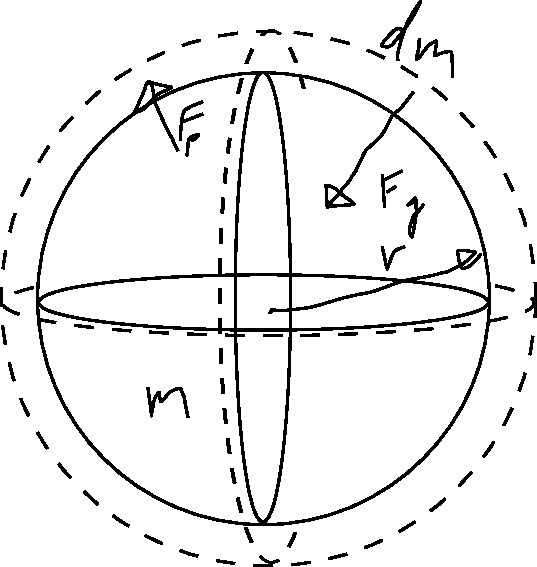
\includegraphics[width=0.32\textwidth]{figurer/hydrostatic_equillibrium.pdf}
    \caption{Kladd: The forces acting on a thin shell $\dd m$.}
    \label{fig: hydrostatic equillibrium}
\end{figure}

Both the Newtonian limit and the TOV equation are equations of \emph{hydrostatic equilibrium}, where the forces on a small volume of the fluid cancel out.
In the case of the TOV equation, we tacitly assumed hydrostatic equilibrium when we gave the fluid a rest frame where we could write $v_\mu = (v_0, 0, 0, 0)$ globally.
We can eliminate the equation for mass by differentiating \autoref{Newtonian limit TOV} with respect to $\tilde r$.
This gives us a single equation for hydrostatic equilibrium in the Newtonian limit,
%
\begin{equation}
    \label{Newtonian limit TOV single equation}
    \odv{}{\tilde r} 
    \left( \frac{\tilde r^2}{\tilde u} \odv{\tilde p}{\tilde r}\right) 
    = -  k'' \tilde r^2  \tilde u, \quad
    k'' = 3 \frac{k_2 k_1}{k_3} = 4 \pi G \frac{u_0^2 r^2_0}{p_0}.
\end{equation}
This is a second order differential equation, so we need an new boundary condition in addition to $p(0) = p_c$.
Close to the center, we can see from \autoref{Newtonian limit TOV} that for a finite energy density, we must have $p'(0) = 0$, our second boundary condition.

One important model for stars is the \emph{polytrope}, which has an equation of state of the form $u = K p^\gamma$ for some constant $K$.
As we will see, this fits well as the Newtonian limit of many equations of state and can be used to make predictions such as the Chandrasekhar limit, which sets the upper limit of the mass of white dwarf stars to $M \approx 1.5 \, M_\odot$~\autocite{chandrasekharHighlyCollapsedConfigurations1935,glendenningCompactStarsNuclear2012}.
To write \autoref{Newtonian limit TOV single equation} on the standard form, we assume $\gamma \neq 1$ and introduce
%
\begin{equation}
    \tilde u = a \theta^{n}, \quad 
    n = \frac{1}{\gamma - 1}, \quad 
    a = \frac{u(p_c)}{u_0}, 
    \quad a^{\frac{\gamma - 2}{2}}C \xi = r, \quad 
    C =\sqrt{ \frac{K}{k''} \frac{\gamma}{\gamma - 1}}.
\end{equation}
%
$n$ is called the \emph{polytropic index} of the star.
Inserting these new variables into the equation of hydrostatic equilibrium gives
%
\begin{equation}
    \label{Lane Emden equation}
    \frac{1}{\xi^2} \odv{}{\xi} \left(\xi^2 \odv{\theta}{\xi} \right) + \theta^n = 0.
\end{equation}
%
This is called the Lane-Emden equation and was first used to model stars as early as 1870~\autocite{laneTheoreticalTemperatureSun1870}.
The boundary conditions $p(0) = p_c$ and $p'(0) = 0$ now read $\theta(0) = 1$ and $\theta'(0) = 0$.
The stellar radius is defined by the first zero of the Lane-Emden function above $\xi = 0$, $\theta(\xi_1) = 0$, so that
%
\begin{equation}
    \label{Radius polytrope}
    \frac{R}{r_0}= C \xi_1  a^{\frac{\gamma-2}{2}}. 
\end{equation}
%
The total mass of the star can be integrated using \autoref{mass relation dimensionless} and \autoref{Lane Emden equation},
%
\begin{equation}
    \frac{M}{m_0} = 3 k_2 a^{\frac{3\gamma-4}{2}} C^3 \int^{\xi_1}_0 \dd \xi \, \xi^2 \theta^n = [-3 k_2 \xi_1^2 \theta'(\xi_1)] a^{\frac{3\gamma-4}{2}}.
\end{equation}
%
Thus, given a specific equation of state, and thus $\gamma$, the mass-radius relationship is given by
%
\begin{equation}
    \label{Polytrope mass radius relationship}
    R \propto M^\beta, \quad \beta = {\frac{\gamma - 2}{3 \gamma - 4}}.
\end{equation}
%
\autoref{fig: mass radius relation polytropes} illustrates this relationship, in arbitrary units, for a series of different values of $\gamma$, as well as the dependence of $\beta$ on $\gamma$.
For most values of $\gamma$, the stellar radius will increase as the mass increases.
The only range within which the radius decrease as the mass increase is $\gamma \in \left(\frac{4}{3}, 2 \right)$.
At $\gamma = \frac{4}{3}$ and $\gamma = 2$, respectively the mass and radius become independent of the central density.
If included in our figure, these polytropes would correspond to a horizontal and a vertical line.
\todo[inline]{what about $\gamma = 1$?}

\begin{figure}[h]
    \centering
    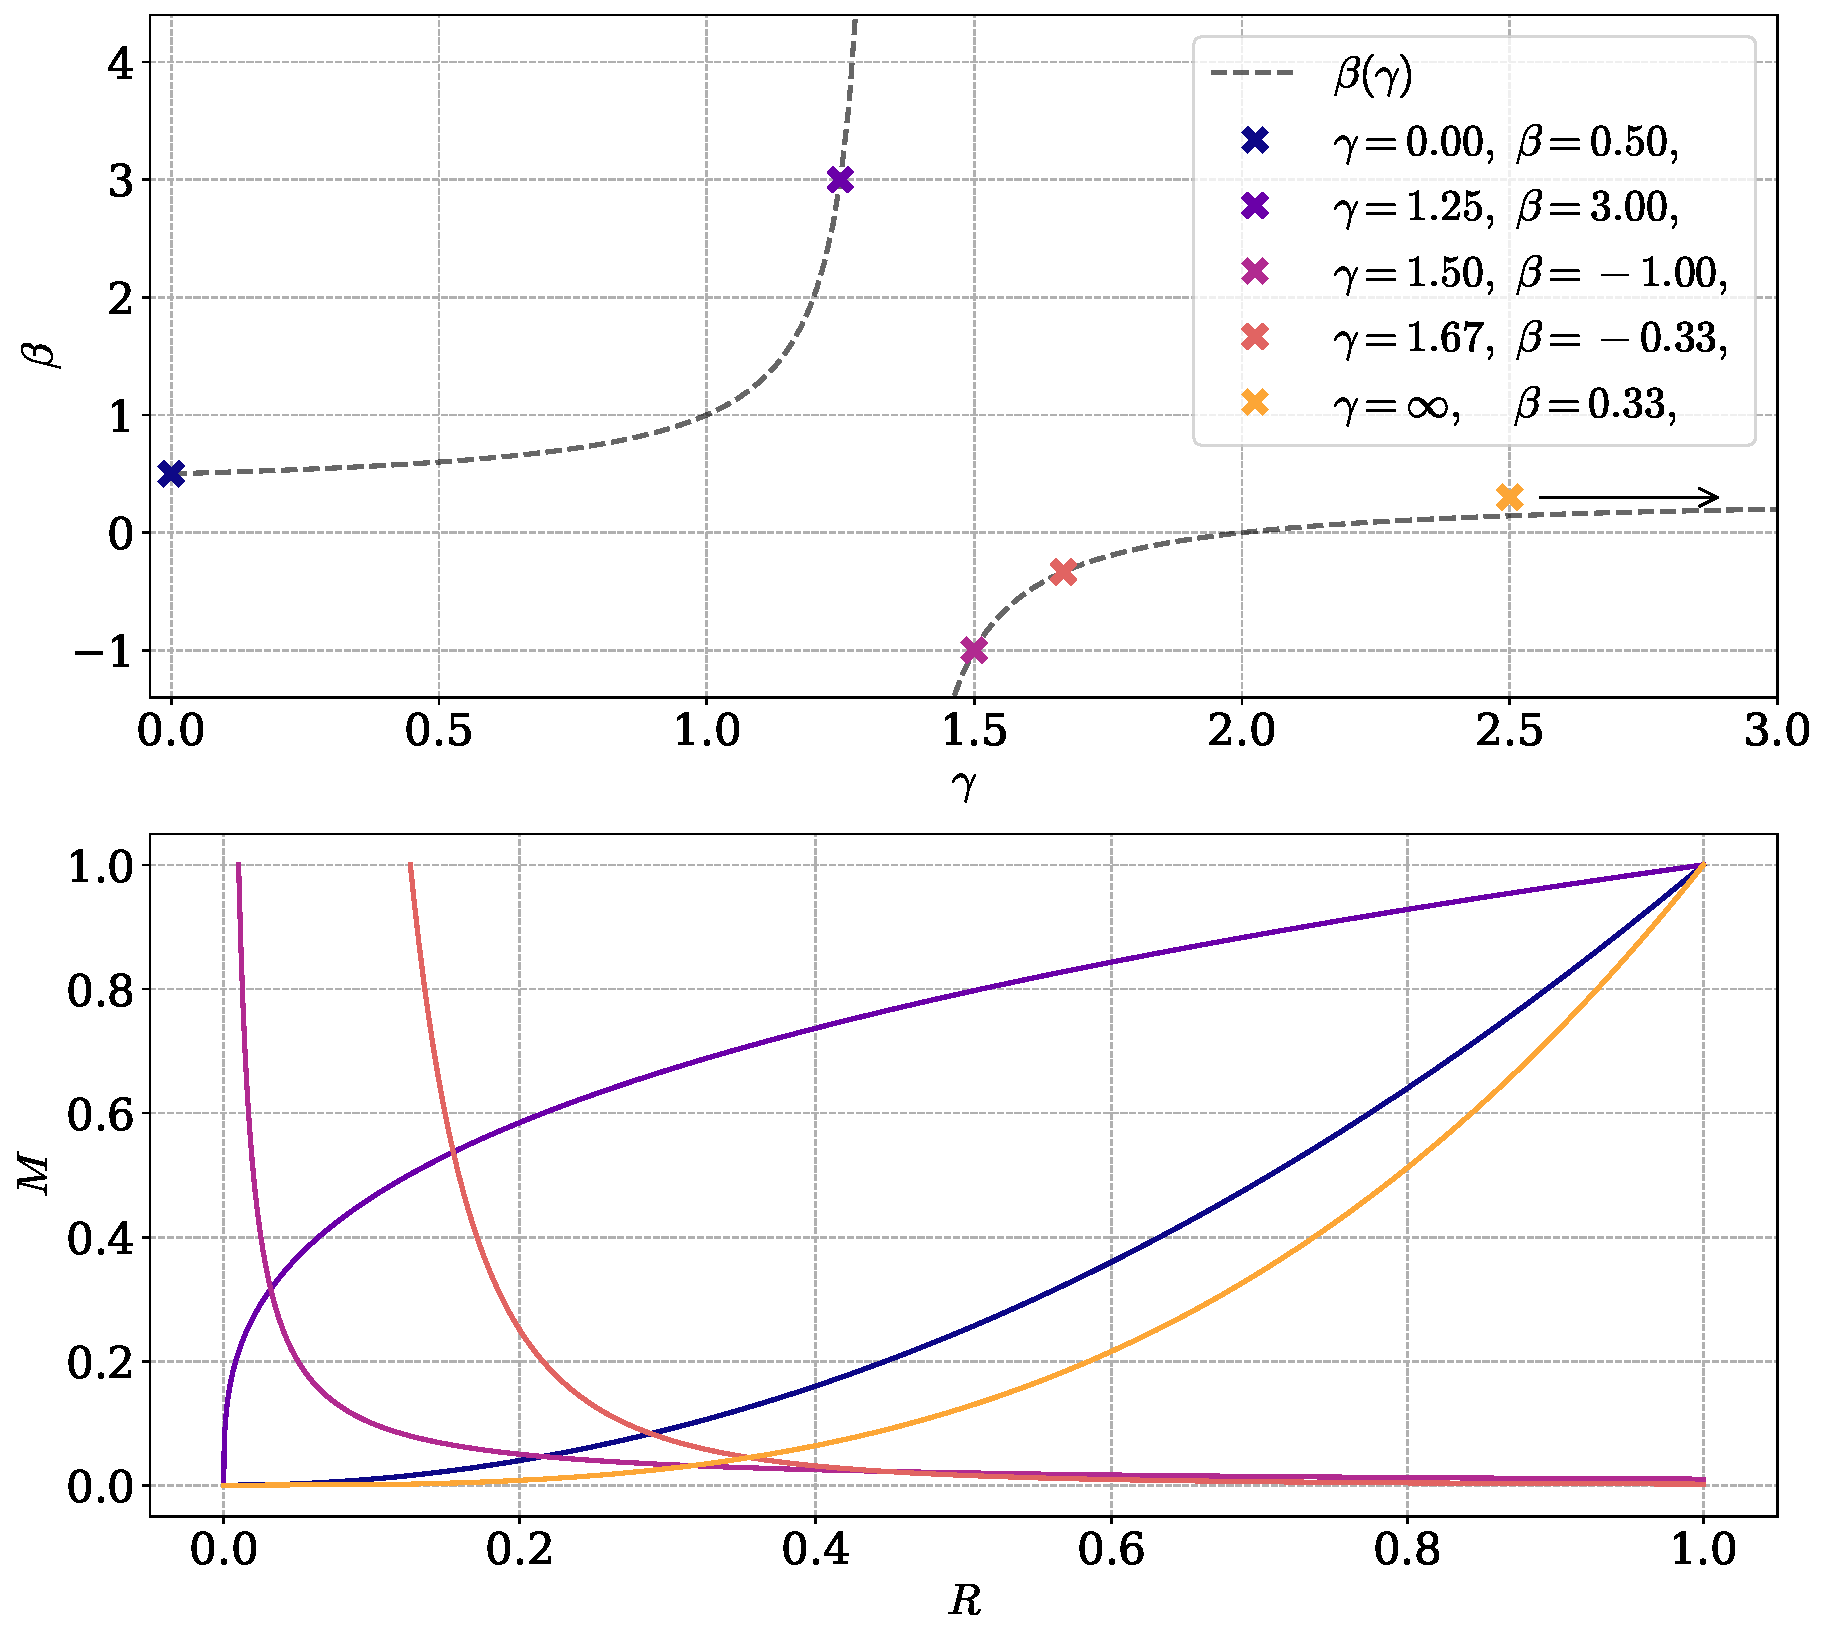
\includegraphics[width=\textwidth]{../scripts/figurer/mass_radius_relation_polytropes.pdf}
    \caption{
        Left: The dependence of $\beta$ on $\gamma$, together with a selection of points.
        Top: The mass-radius relation, in arbitrary units, for polytropes corresponding to the selected points on the left side. The color of the lines indicate which point it corresponds to.
        }
    \label{fig: mass radius relation polytropes} 
\end{figure}



\subsection{Incompressible fluid}
\label{subsection: incompressible fluid}

The simplest model for a star is one made up of an incompressible fluid, where the energy density is independent of the pressure.
This corresponds to a polytrope with $\gamma = \infty$.
In this case, the energy density of the star will be constant for a radius $r < R$, before it drops to zero,
%
\begin{equation}
    u(r) = u_0 \, \theta (R- r),
\end{equation}
%
where $u_0$ is a constant and $\theta(x)$ the Heaviside step function.
We choose $r_0 = R$.
Inserting this into the differential equation of the mass function, \autoref{mass relation dimensionless}, together with the boundary condition $m(0) = 0$, yields
%
\begin{equation}
    \tilde m(\tilde r) = k_2 \tilde r^3,
\end{equation}
%
when $r < R$.
For $r \geq R$, or $\tilde r \geq 1$, this relationship is simply constant $\tilde m(\tilde r) = \tilde m(1) = k_2$.
We choose $m_0$ to be the gravitational mass of the star, $M = \frac{4 \pi }{3} R^3 u_0$, which is equivalent to setting $k_2 = 1$.
Lastly, we choose $u_0 = p_0$, so that $k_3 = 1$.
With this the TOV equation, \autoref{TOV dimensionless}, becomes
%
\begin{equation} 
    \odv{\tilde p}{\tilde r} 
    = - k_1 \tilde r 
    \frac{(1 + \tilde p)(1 + 3 \tilde p)}{(1 - 2 k_1 \tilde r^2)}.
\end{equation}
%
This is a separable ODE, and each variable may be integrated separately.
Using
%
\begin{align}
    \int \frac{\dd x}{(1 + x)(1 + 3x)}
    = \frac{1}{2} \ln \frac{3x + 1}{x + 1} + \const , \quad
    \int \dd x \frac{x}{1 - 2 x^2} 
    = \frac{1}{4}\ln\left(1 - 2 x^2 \right)
    + \const,
\end{align}
%
together with the boundary condition $p(r = R) = 0$, we get 
%
\begin{equation}
    \label{pressure afo r incompressible}
    \tilde p(\tilde r) 
    = 
    - \frac{\sqrt{1 - 2 k_1} - \sqrt{1 - 2 k_1 \tilde r^2}}
    {3 \sqrt{1 - 2 k_1 } - \sqrt{1 - 2 k_1 \tilde r^2}}.
\end{equation}
%
We see that the star is entirely characterized by $k_1$.
In \autoref{fig: pressure incompressible fluid}, we have plotted the pressure as a function of radius for some values of $k_1$.
As $k_1$ approaches $0.\bar 4 = 4/9$, the pressure at the center of the star increases rapidly.
From the denominator of \autoref{pressure afo r incompressible} at $r\rightarrow 0$, we find the limit
%
\begin{equation}
    \label{mass radius constraint}
    k_1 = G \frac{M}{R} < \frac{4}{9}
\end{equation}
%
for the pressure to remain finite.
This is an absolute limit of the mass of an object given its radius or vice versa.
Although this limit is derived for a particular, unrealistic case, the more general statement can be shown to hold.
General relativity does not allow for a static solution with energy densities greater than this limit; any such configuration would collapse~\autocite{carrollSpacetimeGeometryIntroduction2019}.


\begin{figure}[h]
    \centering
    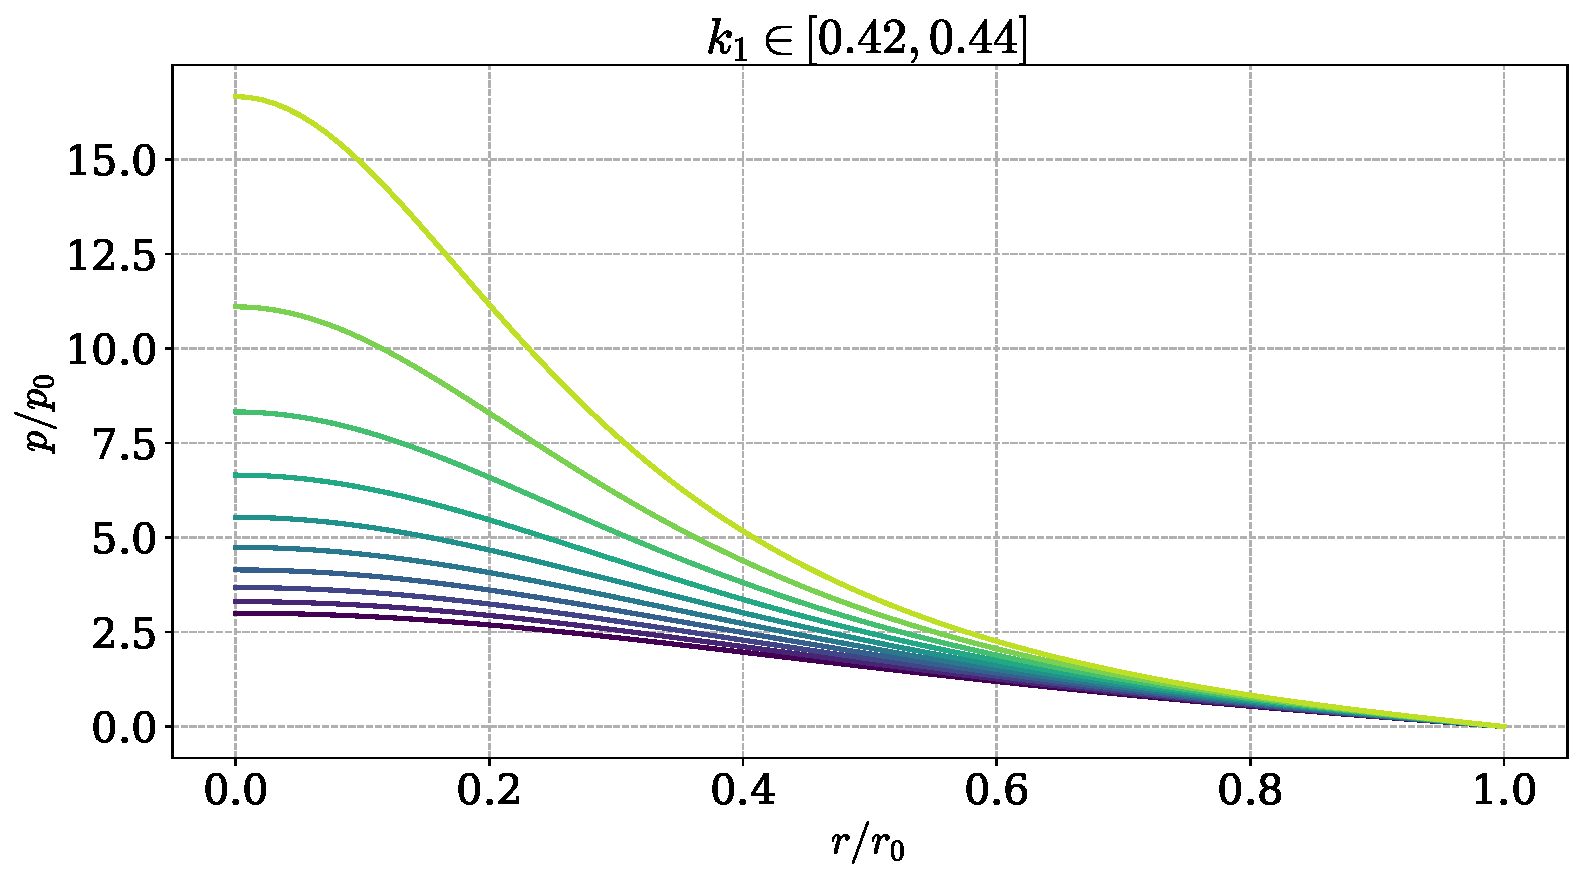
\includegraphics[width=0.8\textwidth]{../scripts/figurer/incompressible.pdf}
    \caption{The pressure in units of $p_0$, as a function of the radius, in units of $r_0$. The graphs with lighter color and higher pressure at $r = 0$ corresponds to higher values of $k_1$. The values of $k_1$ are linearly spaced.}
    \label{fig: pressure incompressible fluid}
\end{figure}

 
If we expand the solution \autoref{pressure afo r incompressible} in powers of $k_1$, then the leading order contribution is
%
\begin{equation}
    \tilde p(r) = \frac{1}{2} k_1 (1 - \tilde r^2).
\end{equation}
%
This is the Newtonian limit.
As a cross-check, we see that this solution obeys the equation of hydrostatic equillibrium in this limit, \autoref{Newtonian limit TOV}, as $\tilde u = 1$ and $k_2 = k_1 = 1$.
This is the general solution for an incompressible fluid in Newtonian gravity.
This solution does not have any upper limit for $k_1$; the limit $M/R < 4 / 9$ is purely relativistic phenomenon.
In \autoref{fig: pressure incompressible fluid newtonian}, the Newtonian approximation is compared to the full, relativistic solution.
We see that the Newtonian approximation is highly accurate for $k_1$ less than around $0.01$.


\begin{figure}[h]
    \centering
    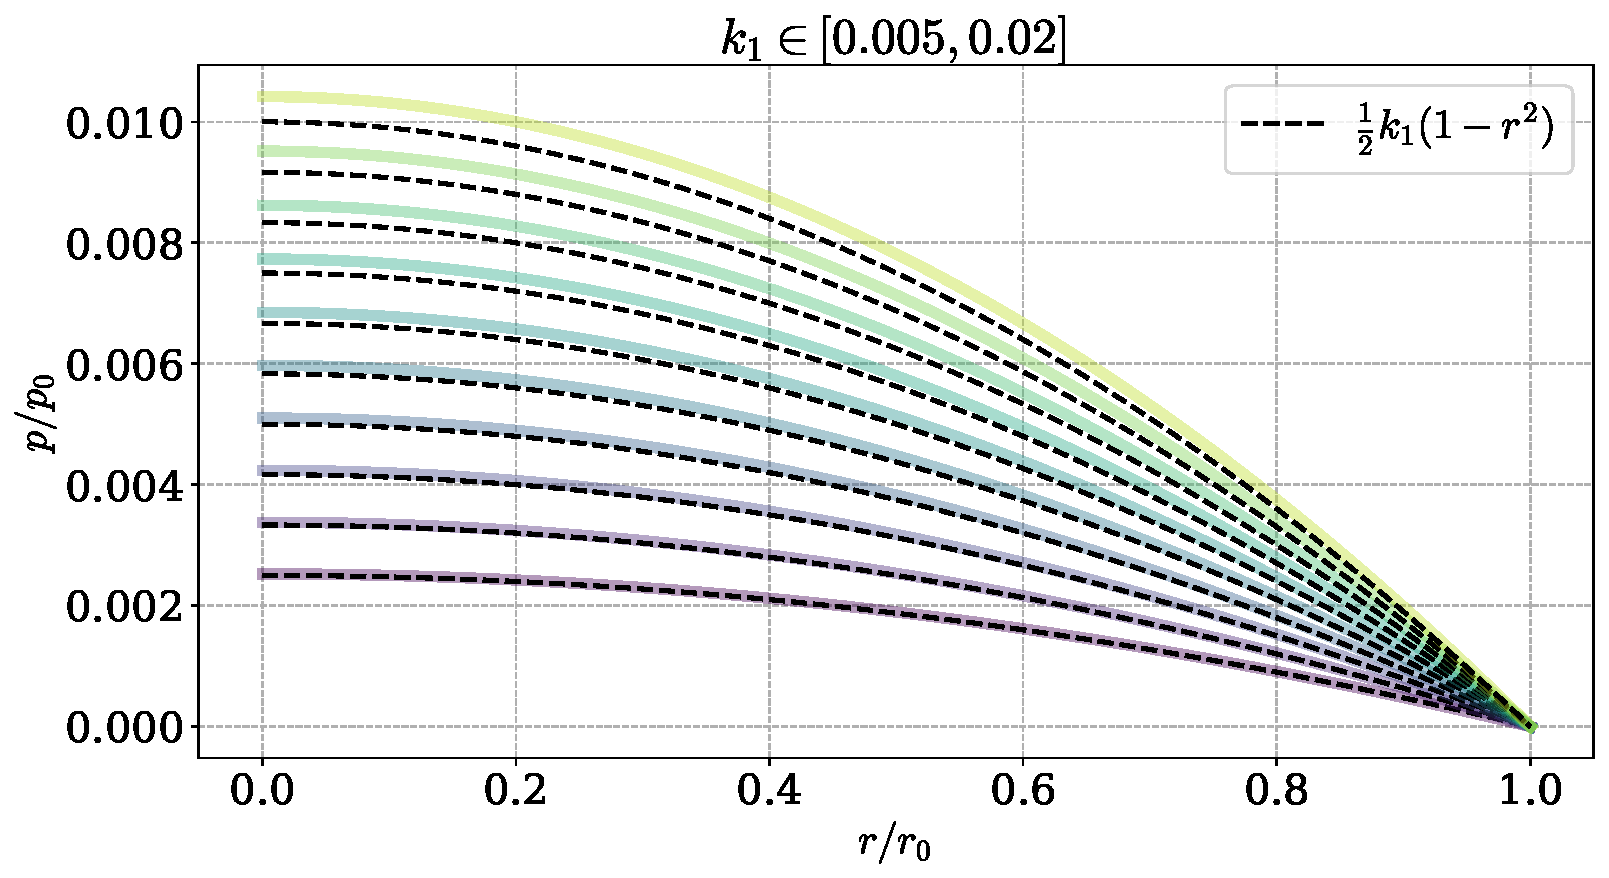
\includegraphics[width=0.8\textwidth]{../scripts/figurer/incompressible_newt.pdf}
    \caption{The pressure in units of $p_0$, as a function of the radius, in units of $r_0$. The wide, colored lines correspond to the full relativistic solution, while the dashed lines is the Newtonian approximation, for the same value of $k_1$. The values of $k_1$ are linearly spaced.  }
    \label{fig: pressure incompressible fluid newtonian}
\end{figure}


    \section{A star of cold, non-interacting fermions}
\label{section: cold fermi star}

This section is based on~\autocite{glendenningCompactStarsNuclear2012,andersenIntroductionStatisticalMechanics2012,kapustaFiniteTemperatureFieldTheory2006}.

In this section, we will study a simple model of a star made up of non-interacting, cold neutrons.
This is one of the earliest models used to study neutron stars, the remenants of massive stars~\autocite{glendenningCompactStarsNuclear2012}.
For this model, we use results derived in \autoref{section: fermions}.



\subsection{Thermodynamics and the equation of state}

The total energy $U$ is related to the grand canonical free energy $F$ by a Legendre transformation,
%
\begin{equation}
    F(T, V, \mu) = U - T S - \mu Q, \quad \dd F = - S \dd T - p \dd V - Q \dd \mu.
\end{equation}
%
Here $T = {1}/{\beta}$ is temperature, and $S$ entropy,  $p$ pressure, and $V$ volume.
$Q$ is some conserved charge, in our case the number of particles minus antiparticles, and $\mu$ is the corresponding chemical potential.
These thermodynamic variables are related to the free energy by
%
\begin{equation}
    S = - \pdv{F}{T} = \beta^2 \pdv{F}{\beta}, \quad
    Q = - \pdv{F}{\mu}, \quad
    p = - \pdv{F}{V}.
\end{equation}
%
When the free energy can be written as $F = V \Eff$, where the free energy density $\Eff$ is independent of the volume $V$, then $\Eff = - p$ and
%
\begin{equation}
    \dd (V \Eff) = V \dd \Eff - p \dd V,
\end{equation}
%
allowing us to write
%
\begin{equation}
    \Eff(T, \mu) = u - Ts - \mu n, \quad
    \dd \Eff = -s \dd T - n \dd \mu,
\end{equation}
% 
where $s$ and $n$ are entropy and charge density, defined by
%
\begin{equation}
    s = - \pdv{\Eff}{T} = \beta^2 \pdv{\Eff}{\beta}, \quad
    n = - \pdv{\Eff}{\mu}.
\end{equation}
%
With this, we can write the energy density as~\autocite{andersenIntroductionStatisticalMechanics2012}
%
\begin{equation}
    u = \pdv{}{\beta} \left(\beta \Eff\right) + \mu n.
\end{equation}
%

We calculate the free energy density of non-interacting fermions in \autoref{section: fermions}, with the result \autoref{free energy fermions},
%
\begin{equation}
    \Eff = - 
    \frac{2}{\beta}\int \frac{\dd^3 p}{(2 \pi)^3} 
    \left[
        \beta \omega
        +
        \ln\left(1 + e^{-\beta(\omega - \mu)}\right)
        + 
        \ln\left(1 + e^{-\beta(\omega + \mu)}\right)
    \right],
\end{equation}
%
where $\omega = \sqrt{p^2 + m^2}$.
The first term in the integral is the divergent vacuum energy, which must be renormalized.
We can drop this term; it does not have any observable effects on our results, as we are interested in relative pressure and energy density.
With this, we find the charge density
%
\begin{equation}
    n = \frac{1}{\pi^2} \int \frac{\dd^3 p}{(2 \pi)^3} [n_f(\omega - \mu) - n_f(\omega + \mu)],
\end{equation}
%
where
%
\begin{equation}
    n_f(\omega) = \frac{1}{e^{\beta \omega} + 1}.
\end{equation}
%
is the Fermi-Dirac distribution.
Using this, we find that the energy density is
%
\begin{equation}
    \label{energy density}
    u = \frac{1}{\pi^2} \int_0^\infty \dd p\, p^2 \, \omega \, [n_f(\omega - \mu) + n_f(\omega + \mu)].
\end{equation}
%
As expected, this is the energy per mode times the density of states, integrated over all modes.
To write the pressure, $p = - \Eff$ in terms of an integral over the Fermi-Dirac distribution, we integrate by parts.
We have
%
\begin{equation}
    \int_0^\infty \dd p \, p^2 \ln\left[1 + e^{-\beta(\omega \pm m)}\right]
    = 
    \frac{1}{3} p^3\ln\left[1 + e^{-\beta(\omega \pm m)}\right] \bigg |_0^\infty
    + 
    \frac{1}{3} \int_0^\infty \dd p \, \frac{ \beta p^4}{\omega}n_f(\omega \pm \mu),
\end{equation}
%
where the boundary term vanishes.
This allows us to write the pressure as 
%
\begin{equation}
    \label{pressure}
    p = \frac{1}{3} \int_0^\infty \dd p \, \frac{p^4}{\omega} [n_f(\omega - \mu) + n_f(\omega + \mu)]
\end{equation}



We are interested in the $T = 0$ limit.
In this case, the Fermi distribution becomes a step function, $n_f(\omega) = \theta(-\omega)$.
Without loss of generality, we assume that $\mu > 0$, i.e., we are dealing with an abundance of matter compared to anti-matter.
The dispersion relation $\omega = \sqrt{p^2 + m^2}$ is always positivive.
This means that the contribution to thermodynamic quantities from anti-particles vanish, as the integral is multiplied with $n_f(\omega + \mu) = \theta(-\omega - \mu)$, where the argument $-\omega - \mu$ is strictly negative on the domain of integration.
At zero temperature, the only dynamics are due to the degeneracy pressure of the fermions, that is, due to the Pauli exclusion principle.
There are no thermal fluctuations that can create a particle-antiparticle pair.
Thus, if the system has a positive chemical potential, it will contain no antiparticles.
Furthermore, if $\mu< m$, then integrand multiplied with $n_f(\omega - \mu)$ is also zero in the whole domain of integration.
It is only when $\mu\geq m$ that it is energetically favorable for the system to be in a state with particles.
We define the Fermi momentum $p_f$ by $\mu = \sqrt{\smash{p_f}^2 + m^2}$. 
In the zero-temperature limit, we can then rewrite any integral over the Fermi distribution as
%
%
\begin{equation}
    \int_0^\infty \dd p \, [f(p) n_f(\omega - \mu) + g(p) n_f(\omega - \mu)]= \int_0^{p_f} \dd p \, f(p).
\end{equation}
%
The charge density is thus
%
\begin{equation}
    n = \frac{1}{\pi^2} \int_0^{p_f} \dd p\, p^2 = \frac{p_f^3}{3 \pi^2}.
\end{equation}
%
At $T = 0$, this is the particle number density, as there are no antiparticles.
This density is given by the chemical potential and vanishes when $\mu \leq m$, i.e. when the free energy cost of creating a particle is positive.
We can write the energy density and pressure integrals, \autoref{energy density} and \autoref{pressure}, as
%
\begin{align}
    u &= \frac{1}{\pi^2} \int_0^{p_f} \dd p \,
    p^2 \sqrt{p^2 + m^2}
    = \frac{m^4}{\pi^2} \int_0^{x_f} \dd x \, x^2 \sqrt{x^2 + 1}, \\
    p & = \frac{1}{3 \pi^2} \int_0^{p_f} \dd p \,  \frac{p^4}{\sqrt{p^2 + m^2}} 
    = \frac{m^4}{3 \pi^2} \int_0^{x_f} \frac{\dd x \, x^4}{\sqrt{x^2 + 1}}.
\end{align}
% 
We have defined $x = p / m$ and $x_f = p_f/m$.
These integrals can be evaluated exactly as
%
\begin{align}
    \int_0^a \dd x \, x^2 \sqrt{x^2 + 1} 
    & = \frac{1}{8} 
    \left[\sqrt{a^4 + 1}(2 a^3 + a) - \arcsinh\left(a\right)\right], \\
    \int_0^a \dd x \, \frac{x^4}{\sqrt{x^2 + 1} }
    & = \frac{1}{8} 
    \left[\sqrt{a^2 + 1}(2 a^3 - 3a) + 3\arcsinh\left(a\right)\right].
\end{align}
%
We introduce the characteristic energy and number density,
% 
\begin{equation}
    u_0 = \frac{m^4}{8 \pi^2}, \quad n_0 = \frac{u_0}{m},
\end{equation}
%
which allows us to write the thermodynamic variables as
%
\begin{align}
    \label{Fermi gas particle density}
    n &= \frac{8}{3}  n_0 \,x_f^3 \\
    \label{Fermi gas energy density}
    u &= u_0
    \left[(2x_f^3 + x_f) \sqrt{1 + x_f^2} - \arcsinh\left(x_f\right)\right], \\
    \label{Fermi gas pressure}
    p &= \frac{u_0}{3}
    \left[(2x_f^3 - 3x_f) \sqrt{1 + x_f^2} + 3\arcsinh\left(x_f\right)\right].
\end{align}
%
We have thus chosen $u_0 = p_0$, or equivalently set $k_3 = 1$.
This is natural in the case of a relativistic fluid.




\subsection{Limits}

In the non-relativistic limit, as the chemical potential approaches $m$ and thus $p_f \ll m$, the lowest order contributions to the energy density and pressure are given by the Taylor series around $x_f = 0$,
%
\begin{align}
    \tilde u(x_f) &= \frac{8}{3}x_f^3 + \frac{4}{5} x_f^5 + \Oh(x_f^7),  \\
    \tilde p(x_f) &= \frac{8}{15}x_f^5 + \Oh(x_f^7).
\end{align}
%
By neglecting terms of order $x_f^7$ and higher, we can write this as
%
\begin{equation}
    \tilde u = \tilde n + \frac{4}{5} \left( \frac{8}{3} \tilde n \right)^{5/3},
    \quad
    \tilde p =  \frac{8}{15} \left( \frac{8}{3} \tilde n \right)^{5/3}.
\end{equation}
%
The leading order contribution to the energy density is the rest mass of the particles.
This term does not contribute to the pressure.
As discussed earlier, the non-relativistic limit corresponds to $k_3 \ll 1$, if we chose units so that $\tilde u \approx \tilde p$, or $\tilde u \gg \tilde p$ if we demand that $k_3 = 1$.
We see that $x_f \rightarrow 0$ corresponds to the latter case.
By including only the leading order term, we can eliminate the Fermi momentum and write the equation of state in the non-relativistic limit as $u_{\mathrm{nr}} = k p^\frac{3}{5}$ where $k = 8/3 \cdot (15/8)^{3/5}$.
The non-relativistic approximation of the cold fermions is thus a polytrope with $\gamma = \frac{5}{3}$.
As we see from \autoref{fig: mass radius relation polytropes}, this is within the range where the mass decreases with the size of the star.

In the ultrarelativistic limit, where $p_f \gg m$, the leading order contributions to the pressure and energy density are
%
\begin{equation}
    \tilde u = 2 x_f^4, \quad \tilde p = \frac{2}{3} x_f^4, 
\end{equation}
%
and we get the particularly simple equation of state for the ultrarelativistic limit, $ u_{\mathrm{ur}} = 3 p $, which we recognize as the formula for radiation pressure.
The equation of state $\tilde u(\tilde p)$ in two different regimes are shown in \autoref{fig: equation of state fermi fluid}.
The full equation of state is compared to the non-relativistic and ultrarelativistic approximations.

\begin{figure}[h]
    \centering
    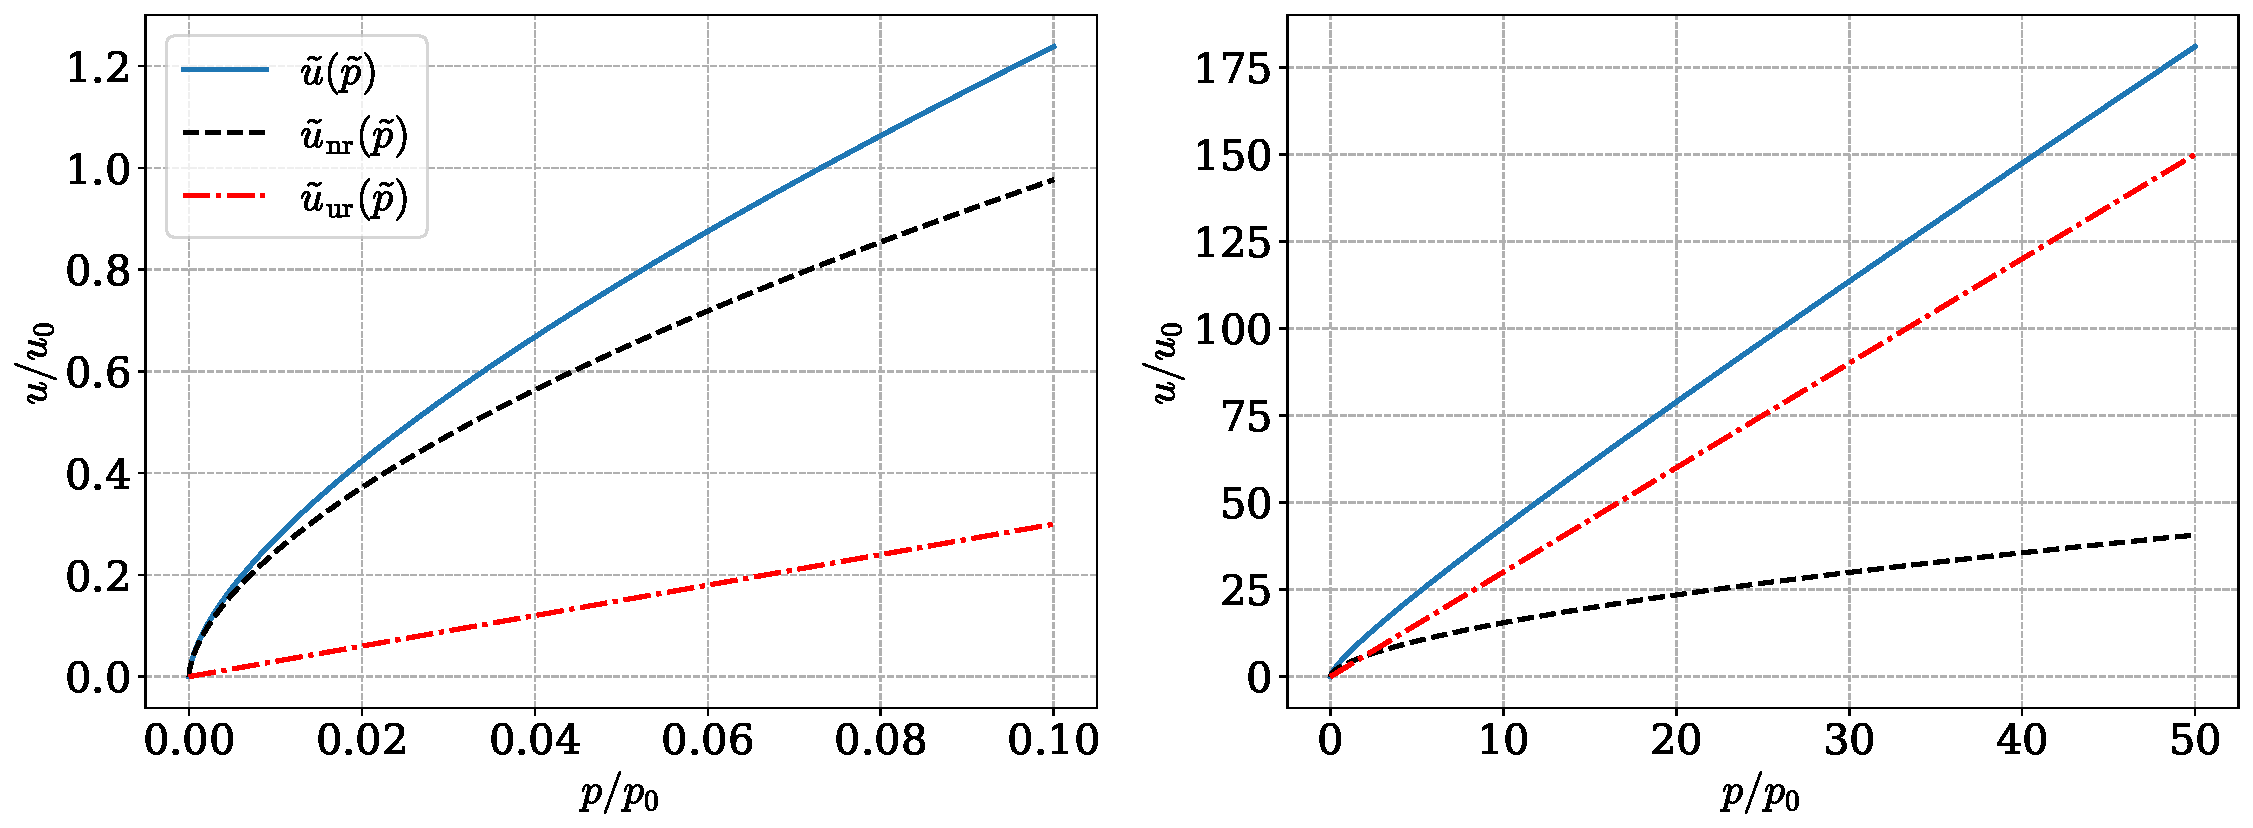
\includegraphics[width=\textwidth]{../scripts/figurer/fermi_eos.pdf}
    \caption{The equation of state of a cold Fermi gas. Both pressure and energy density is normalized to their characteristic quantities, $p_0$ and $u_0$. The equation of state is compared to the non-relativistic approximation, $\tilde u_{\mathrm{nr}}$ as well as the ultrarelativistic approximation, $\tilde u_{\mathrm{ur}}$, in two different regimes.}
    \label{fig: equation of state fermi fluid}
\end{figure}




\subsection{Units}

The equation of state has given us the characteristic energy density and pressure, $u_0$ and $p_0$. 
If we demand
%
\begin{equation}
    G \frac{m_0}{r_0} = \frac{4 \pi }{3}\frac{r_0^3 u_0}{m_0} = 1,
\end{equation}
%
we have two equations and two unknowns, $m_0$ and $r_0$.
This thus defines a complete set of units.
We are using the cold Fermi-gas as a model for a neutron star, an the mass of the fermion $m$ is therefore the neutron mass, \autoref{mass of neutron}, $m_N = 1.674 \cdot 10^{-27} \, \text{kg}$.
After reinstating $\hbar$ and $c$ in metric units, we get
%
\begin{align}
    u_0 &= p_0 = \frac{m^4}{8 \pi^2}\frac{c^5}{\hbar^3} 
    = 2.056\cdot10^{35}  \, \text{J}\,\text{m}^{-3}, \\
    m_0 &= \frac{c^4}{\sqrt{\frac{4 \pi}{3} u_0 G^3} }
    = 1.598 \cdot 10^{31} \, \text{kg}
    = 8.032 \, M_\odot, \\
    r_0 &= \frac{G m_0}{c^2} = 11.86 \, \text{km}. % sjekk
\end{align}
%
From this, we expect our star to have a mass of the order of a solar mass $M_\odot$ and a radius of the order of kilometers, without solving the TOV equation.




\subsection{Numerical results}



With the energy density, \autoref{Fermi gas energy density}, and pressure, \autoref{Fermi gas pressure}, we can numerically solve the TOV equation given a central pressure $p_c$. 
This is done using an adaptive Runge-Kutta method, with the stop criterion $p(r) = 0$.
Description of the code and where to find it is given in \autoref{appendix: code}.
The top graph in \autoref{fig: pressure and mass as a function of radius} shows the pressure, normalized to the central pressure $p_c$, as a function of radius, normalized to the corresponding stellar radius $R$.
The boundary conditions are logarithmically spaced.
The lower graph in \autoref{fig: pressure and mass as a function of radius} shows the mass, normalized to the total mass $M = m(R)$, as a function of the radius, again normalized to the stellar radius.
As in the case of an incompressible fluid, the pressure follows a half bell-shaped curve, with a peak that becomes narrower as the central pressure increases.
The black dashed line corresponds to the solution with the maximum mass, which will discuss shortly.
We see that the pressure and mass curves change most drastically when the central pressure is higher than that corresponding to the most massive star.

\begin{figure}[H]
    \centering
    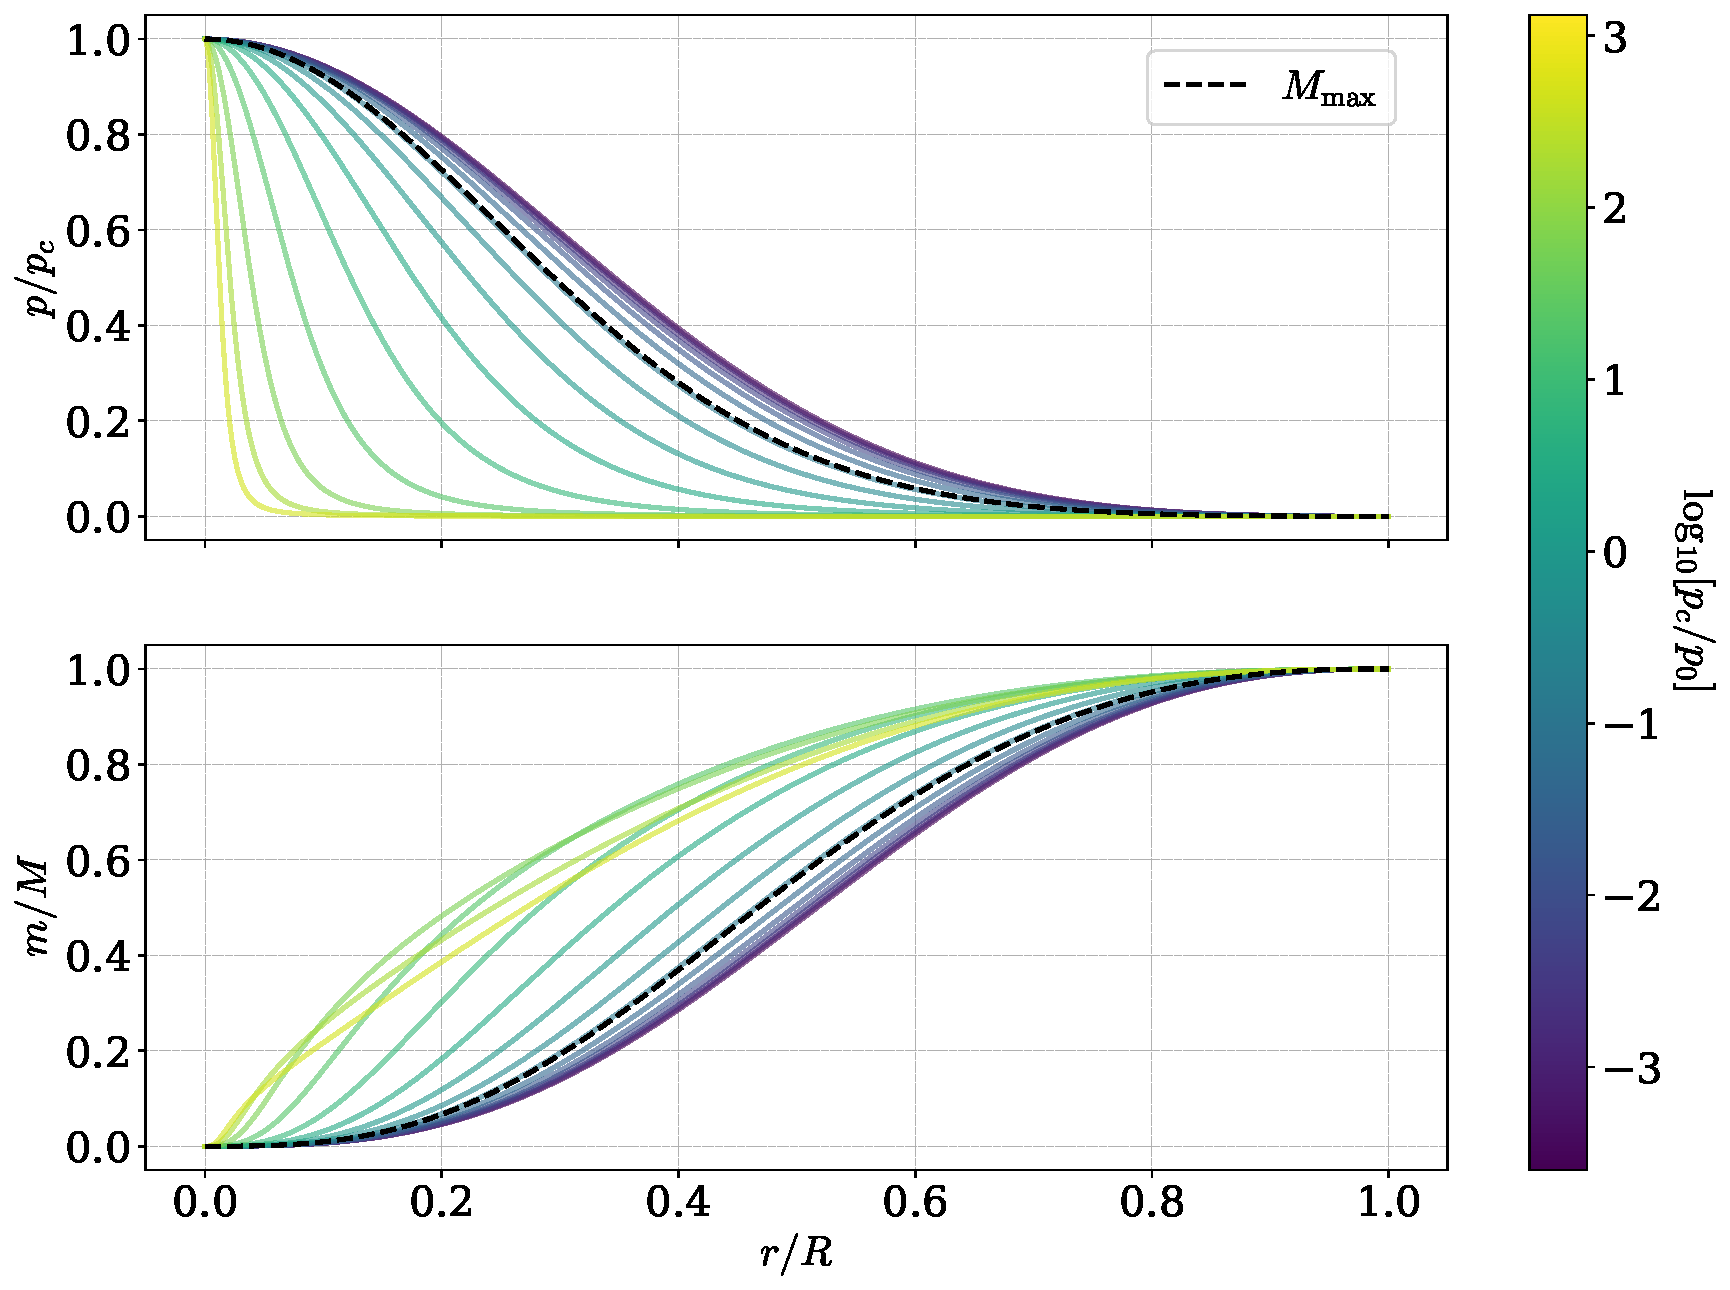
\includegraphics[width=0.9\textwidth]{../scripts/figurer/pressure_mass.pdf}
    \caption{
        Top: The pressure normalized to central value, as a function of radius, normalized to the stellar radius.
        Bottom: The mass normalized to the total mass, as a function of radius, normalized to the stellar radius. 
        This is plotted for several different values of central pressure, which is indicated by the color scheme.
        }
    \label{fig: pressure and mass as a function of radius}
\end{figure}

In \autoref{fig: mass radius relationship fermi gas}, we see the relationship between the mass and radius of the star.
This line is parametrized by the base-10 logarithm of the central pressure, $p(0)$, normalized by $p_0 = u_0$.
The cross marks the maximum mass, $M_\mathrm{max} = 0.711 \, M_\odot$, which corresponds to a radius of $R = 9.20 \, \mathrm{km}$.
This matches the results obtained by Oppenheimer and Volkoff~\cite{oppenheimerMassiveNeutronCores1939}, $M_\mathrm{max} = 0.71$.
In their 1939 paper, Oppenheimer and Volkoff computed five data points in the mass-radius plane.
The results are marked by blue circles in \autoref{fig: mass radius relationship fermi gas}.
We find good agreement between the three points closest to the maximum value and our results.
However, the two results of Oppenheimer and Volkoff furthest away differ significantly from our results.
The black dashed line is the absolute mass-radius constraint, \autoref{mass radius constraint}, and any stable configuration must be on the right side of this line.
As we predicted from looking at the non-relativistic equation of state, the mass decreases with the star's radius, at least for stars with low central pressure.


In \autoref{fig: mass radius relationship comparison}, we compare the mass-radius relationship obtained from the full theory with results from approximations.
The lowest line is obtained by using both the full TOV equation and the exact equation of state.
The next line above is obtained using the non-relativistic equation of state together with the full TOV equation.
The second uppermost line is obtained from the exact equation of state and the Newtonian approximation for the TOV equation.
The uppermost line uses both the Newtonian approximation to the TOV equation and the non-relativistic approximation for the equation of state.
This last line corresponds to a polytrope in Newtonian gravity, as we studied in \autoref{subsection: Newtonian limit and polytropes}.
Unlike the other systems, it does not seem to have an upper limit for the mass, as expected.


\begin{figure}[H]
    \centering
    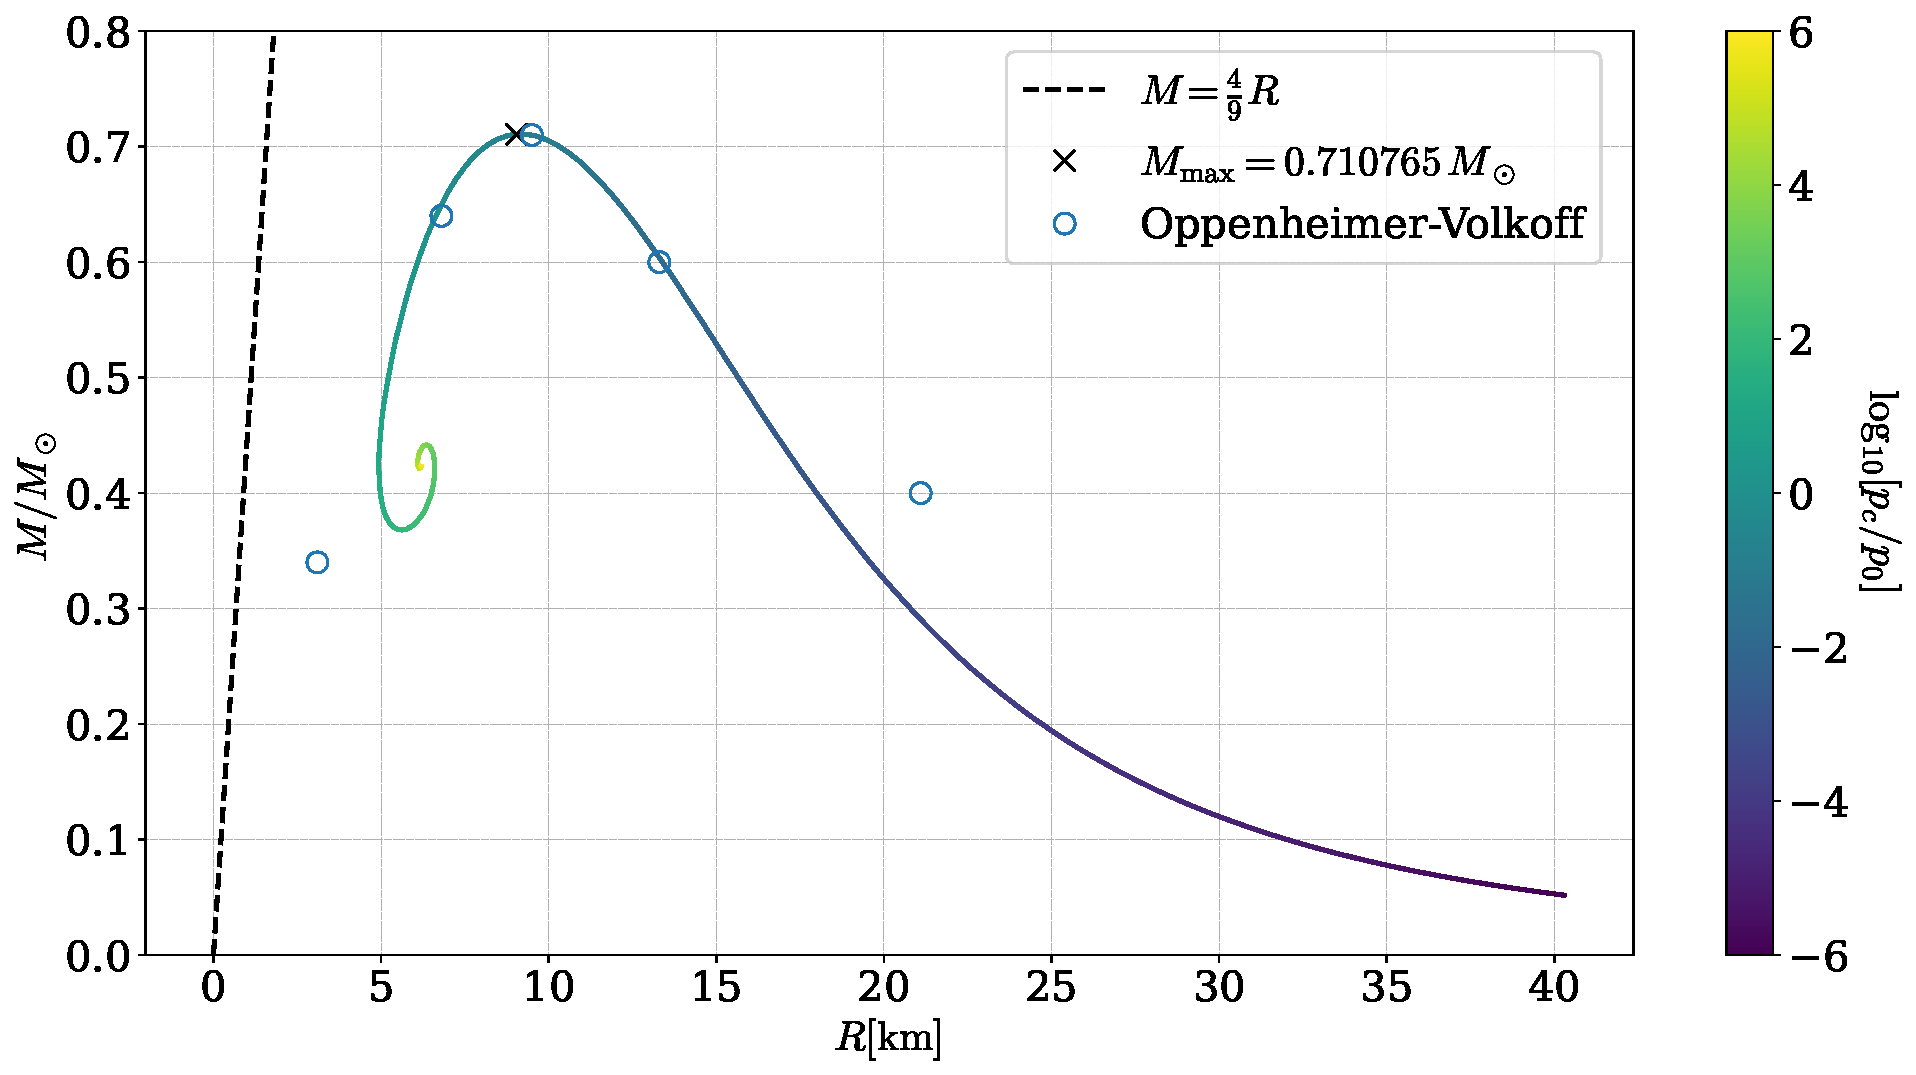
\includegraphics[width=\textwidth]{../scripts/figurer/mass_radius_neutron.pdf}
    \caption{The mass-radius relationship of a star made of a cold gas of neutrons. The line is parametrized by the central pressure $p_c$. The corss indicate the maximum mass solution. The blue circles are results form the 1939 paper of Oppenheimer and Volkoff~\autocite{oppenheimerMassiveNeutronCores1939}.}
    \label{fig: mass radius relationship fermi gas}
\end{figure}

\begin{figure}[H]
    \centering
    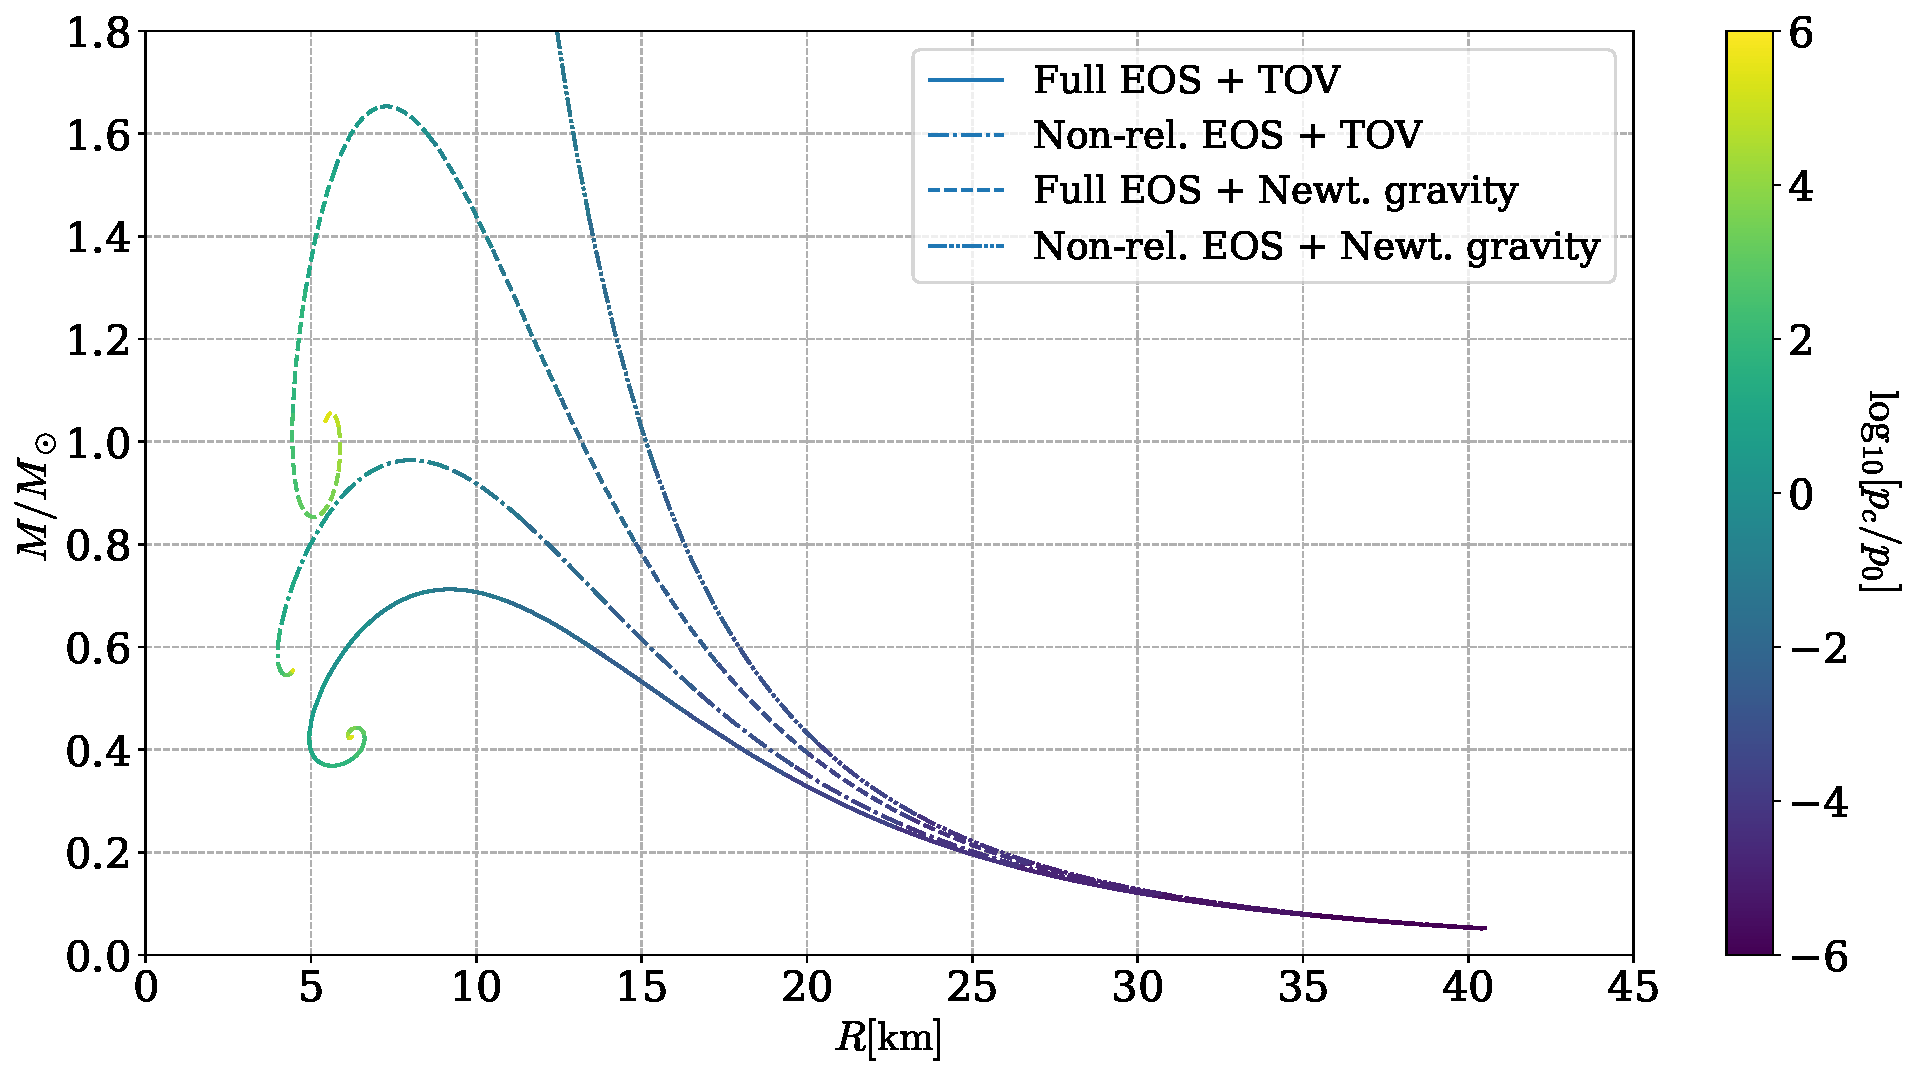
\includegraphics[width=\textwidth]{../scripts/figurer/mass_radius_comparison.pdf}
    \caption{The mass-radius relationship of a cold gas of neutrons. The lowest line is obtained from the TOV equation and full equation of state. The middle line is from the TOV equation and the non-relativistic equation of state. The upper line is obtained from the Newtonian approximation of the TOV equation and the non-relativistic equation of state.}
    \label{fig: mass radius relationship comparison}
\end{figure}




\subsection{Upper bound and stability}
\todo[inline]{Utvid om stability}

For any equation of state, the TOV equation will give a one-parameter\todo{Can there be multiple branches?} family of stars, parametrized by the central pressure $p_c$.
This leads to the possibility of an \emph{absolute maximum} mass for a given equation of state.
In the case of a non-interacting neutron, we found the limit to be $0.71 \, M_\odot$, in agreement with Oppenheimer and Volkoff.
To obtain a more general upper limit for the mass of neutron stars, or compact stars in general, one has to account for more general equations of state.
To constrain the equation of state, we assume firstly that $\odv{p}/{u} \geq 0$.
To justify this, take the non-relativisitc case, $u = n$, in which case the assumption is equivalent to $\odv{p}/{n} \geq 0$.
This says that an increase in particle density, for example, due to compression, will result in a rise in pressure.
This is an instance of Le Chatelier's principle; nature will counteract any change forced upon it.
The speed of sound in the fluid, $v_s$, is given by~\autocite{weinbergGravitationCosmologyPrinciples1972}\todo{Vis dette?}
%
\begin{equation}
    v_s^2 = \odv{p}{u}.
\end{equation}
%
A realistic fluid should not have a speed of sound greater than the speed of light, leading to the constraint $\odv{p}/{u} < 1$.
Using these general assumptions, Rhoades and Ruffini found an upper limit for neutron stars of $3.2 \, M_\odot$~\cite{rhoadesMaximumMassNeutron1974}.

An equation of state with a \emph{high} speed of sound, i.e., with a flat curve in the $p-u$-plane, is called \emph{stiff}.
From \autoref{fig: equation of state fermi fluid}, we see that the Newtonian equation of state is stiffer in the high-energy regime.
The most extreme case is the incompressible model we saw earlier, which breaks causality.
In general, a stiffer equation of state leads to a larger maximum mass.
This is intuitive; the TOV equation describes the balancing of forces from pressure and gravity, and if the pressure raises fast as the density increases, then it can sustain a large total mass before it collapses~\autocite{glendenningCompactStarsNuclear2012}.


Solutions to the TOV equation are systems in hydrostatic equilibrium.
However, as a pen perfectly balances on its edge, this does not imply stability.
When perturbed, a stable system returns back towards its equilibrium position as a marble in the bottom of a bowl.
On the other hand, an unstable system will amplify perturbations, leading to a collapse or an explosion.
We can make an intuitive argument for which configurations for a given family of stars are stable.
We will again assume that the equation of state, on a microscopic level, obeys Le Chatelier's principle in the form $\odv{p}/{n} > 0$.\todo{Er det en god antagelse?}
We can see that this holds for all the cases we are considering.
A star in equilibrium will find itself on the line parametrized by its central pressure, such as \autoref{fig: mass radius relationship fermi gas}.
In this case, a perturbation reducing the radius of the star will increase the central pressure as the particle density increases. \todo{Kan vi være helt sikre på dette?}
This is illustrated in \autoref{fig: fermi stability}.
A star in equilibrium at point A can be compressed to an out-of-equilibrium configuration, point B.
This point has a central pressure corresponding to the equilibrium state at point C.
As the equilibrium configuration at point C has a \emph{lower} mass than the configuration at B, it has a weaker gravitational effect.
Therefore, we would expect it to shrink further, as the central pressure of B is not enough to support its gravitational mass.
This compression will lead to an even higher central pressure.
We thus have a positive feedback loop, and the initial perturbation will continue to grow.
We can make a similar argument in the case where the mass increases with an increase in the central pressure.
Here, a compression will lead to a state in which central pressure corresponds to an equilibrium state with a \emph{higher} mass.
This state will thus tend to expand after a compression, counteracting the perturbation.
This gives us the following criterion for stability,
%
\begin{equation}
    \odv{M}{p_c} > 0.
\end{equation}

\begin{figure}[!h]
    \centering
    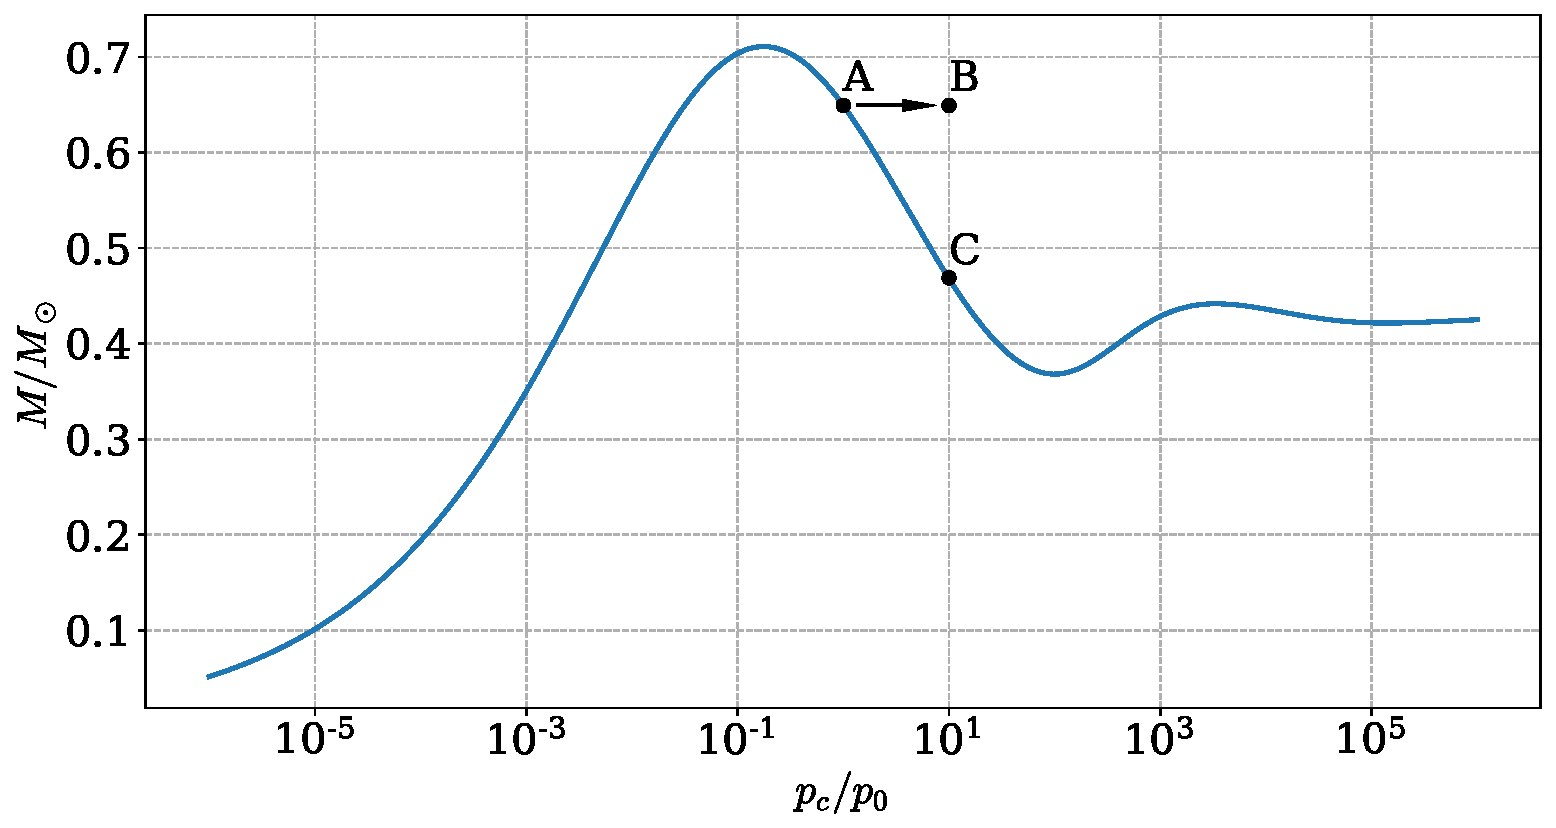
\includegraphics[width=0.7\textwidth]{../scripts/figurer/fermi_stability.pdf}
    \caption{
        The plot shows the mass, in units of solar masses, of a star of a cold gas of neutrons, as a function of the central pressure, normalized to the characteristic pressure.
    Point A denotes a position of equilibrium, which can be compressed to an out-of-equilibrium point, B, which has a central pressure corresponding to an equilibrium configuration, point C.
    }
    \label{fig: fermi stability}
\end{figure}

As it turns out, this is only a necessary requirement for stability.
To conduct a more rigorous study of stability, one must derive the equation of hydrostatic equilibrium with the addition of perturbations as time-dependent, radial oscillations.
This is done by discplacing a fluid elemet at a radius $r$ and time $t$ by $\delta r(r, t) = \sum_n A_n \xi_n(r) e^{i \omega_n t}$.
Here, $\xi_n$ are normal modes with frequencies $\omega_n$, $n \in \{0, 1, ...\}$.
The equation for the eigenmodes was first obtained by Chandrasekhar~\autocite{chandrasekharDynamicalInstabilityGaseous1964}, and can be written in the form of a Sturm-Liouville theory equation,
%
\begin{equation}
    \left[     \odv{}{r} \left( \Pi \odv{}{r}  \right) + Q + \omega_n W \right] \xi_n
    = 0,
\end{equation}
%
where $\Pi$, $Q$, and $W$ are functions of the pressure, energy density, particle density, $\alpha$, and $\beta$.
These quantities are thus given by a solution to the equilibrium problem~\cite{glendenningCompactStarsNuclear2012}.
This analysis is outside the scope of this thesis, but we summarize some important conclusions.
Stability is encoded in the sign of the square of the frequencies.
For $\omega_n^2>0$, the mode will remain oscillatory, while if $\omega_n^2<0$, it will grow exponentially.
Thus, if the system has \emph{any} modes such that $\omega_n^2<0$, it is unstable.
One mode $\omega_n$ will change stability at a critical point on the $M-R$ curve, where
%
\begin{equation}
    \odv{M}{u_c} = 0,
\end{equation}
%
and this will \emph{only} happen at critical points~\autocite{thorneGeneralRelativisticTheoryStellar1968}. Here, $u_c$ is the central energy density corresponding to $p_c$.
This is equivaent to the criterion $\odv{M}/{p_c} = 0$ as long as $\odv{p}/{u}$ is finite.
Whether or not the change is from a stable mode to an unstable one is dependent on whether or not the curve turns clockwise (a mode becomes stable) counterclockwise (a node becomes unstable)~\autocite{thorneGeneralRelativisticTheoryStellar1968}.
We know that very low-pressure, cold fermions are stable, which means that configuration with a radius larger than the maximum mas $0.71 \, M_\odot$ will be stable.
As illustrated in \autoref{fig: mass radius relationship fermi gas}, the curve then turns counterclockwise, and a new mode is made unstable each half turn.


    \chapter{Chrial perturbation theory}
    \label{chapter: chpt}
    In this chapter, we will take the general knowledge from the general theory in \autoref{chapter: QFT} and apply it to the specific case of quantum chromodynamics, which results in \emph{chiral perturbation theory}, or \chpt.

\section{QCD}
This section is based on~\autocite{peskinIntroductionQuantumField1995,schererIntroductionChiralPerturbation2002,schwartzQuantumFieldTheory2013}

\subsection{Yang-Mills theory and Gauge symmetry}


In our discussion on global symmetries, we considered the global transformation of fields by some group $G$.
In gauge theories, we will consider local transformations.
That is, the transformations are themselves functions of spacetime, $U = U(x)$, and take on some value in $G$ for all points in space.
With this, however, we encounter a problem with comparing the value of a field at different points.
As the symmetry is local, a gauge transformation will generally affect the field at two points differently.
We must find a way to compare fields at different points independent of gauge transformations.
This is similar to a problem we have encountered before.
In differential geometry, as described in \autoref{section: differential geometry}, we needed a connection $\Gamma^\rho_{\mu \nu}$ to compare vectors in different tangent spaces in a coordinate independent way.
In gauge theories, we generalize this by defining a connection, $A_\mu$, to compare field values at different points in a gauge-independent way.

Consider a set of $N_c$ fields $\psi_c$, which the symmetry group $\Lie{SU}{N}$ acts linearly on as $\psi_c \rightarrow U_{cc'} \psi_{c'}$.
We can write $U = \exp{i \eta_\alpha T_\alpha}$, where $T_\alpha$ are the generators of $\lie{su}{N_c}_c$, and can therefore be written $A_\mu = A_\mu^\alpha T_\alpha$.
The transformation is then made local by letting the coordinates of $\Lie{SU}{N}$ be functions of spacetime, $\eta_\alpha = \eta_\alpha(x)$.
As we did in \autoref{section: differential geometry}, we define the covariant derivative $D_\mu$ to transform as the thing on which it acts.
It has the form
%
\begin{equation}
    \label{covariant derivative Yang-Mills}
    D_\mu^{cc'} \psi_{c'} = (\delta_{cc'}\partial_\mu - i g A_\mu^{cc'} )\psi_{c'},
\end{equation}
%
where $A_\mu^{cc'}$ is a new, dynamic field, the gauge field.
This field takes values in the Lie algebra of the gauge group, $\lie{su}{N}$.
We will suppress the $c$-indices for cleaner notation.
This field also transform under the gauge group.
By enforcing the transformation rule $D_\mu A_\nu \rightarrow U D_\mu A_\nu$, we can deduce the transformation properties of the gauge field, 
%
\begin{equation}
    \label{Gauge transformation gauge field}
    A_\mu\rightarrow U \left(A_\mu + \frac{i}{g} \partial_\mu\right) U^\dagger
\end{equation}
%
With the covariant derivative, we can create gauge-invariant terms, such as $\bar \psi D_\mu \psi$.
In \autoref{section: differential geometry} we introduced the Riemann tensor as the commutator of covaraint derivatives, \autoref{Riemann tensor}.
This ensures that it transforms as a tensor and gives us the interpretation as a quantity that measures the amount vectors curved when parallel transported in a small loop.
In analogy, we define the \emph{field strength tensor},
%
\begin{equation}
    G_{\mu \nu} := \frac{i}{g} [D_\mu, D_\nu]
    = \partial_\mu A_\nu - \partial_\nu A_\mu - i g[A_\mu, A_\nu].
\end{equation}
%
$A_\mu$ is an element of a Lie algebra, so the commutator is given by the structure constants of that algebra, \autoref{structure constants}.
The field strength tensor transforms as $G_\mu \rightarrow U G_{\mu \nu}U^\dagger$.
This allows us to create gauge-invariant terms of only this tensor, which, as with the Ricci scalar in general relativity, are the building blocks of the Lagrangian of the gauge field.
The lowest order terms are
%
\begin{equation}
    G^{\mu \nu}_\alpha G_{\mu \nu}^\alpha, \quad
    \epsilon^{\mu \nu \rho \sigma} G_{\mu \nu}^\alpha G_{\rho \sigma}^\alpha.
\end{equation}
%
Here, $\alpha$ is the index in $\lie{su}{N}$-space.

\subsection{The QCD Lagrangian}

Quantum chromodynamics, or QCD, is the specific gauge theory of quarks $q_{fc}$, spin-$\frac{1}{2}$ particles, interacting via the strong force, a $\Lie{SU}{3}_c$ gauge field denoted $A_\mu$.
There are six quarks $q$, called flavors and indexed by $f$, with an additional quantum number called color indexed by $c$.
The quarks, labeled u, d, s, c, t, and b, have different masses.
This thesis will include the two or three lightest quarks at different times.
Therefore, we denote the number of flavors by $N_f$.
The Lagrangian of QCD, including only the strong force, is
%
\begin{equation}
    \Ell_{\text{QCD}} 
    = \bar q (i \slashed D - m)q - \frac{1}{4} G_{\mu \nu}^\alpha G^{\mu \nu}_\alpha.
\end{equation}
%
We have suppressed color and flavor indices.
$\slashed D q = \gamma^\mu (\partial_\mu - i g A_\mu) q$ is the covariant derivative associated with the $\Lie{SU}{3}_c$ gauge group with coupling constant $g$, and $\gamma^\mu$ are the Dirac matrices, as described in \autoref{section: algebra bases}.
The quark mass matrix, $m$, acts on the flavor indexes as the flavor states are mass eigenstates.
There are no known symmetries that forbid a $\epsilon^{\mu \nu \rho \sigma} G_{\mu \nu}^\alpha G_{\rho \sigma}^\alpha$-term, and its absence is dubbed the strong CP problem~\autocite{schwartzQuantumFieldTheory2013}.



\subsection{Chiral symmetry}

If we consider the massless QCD Lagrangian, $m = 0$, it has an additional symmetry of rotation in its flavour indices.
We can project the quarks down to their \emph{chiral} components by introducing projection operators
\begin{equation}
    P_R = \frac{1}{2}\left(1 + \gamma^5\right), \quad
    P_L = \frac{1}{2}\left(1 - \gamma^5\right).
\end{equation}
%
Here, $\gamma^5$ is the ``fifth gamma-matrix'', as described in \autoref{section: algebra bases}.
As good projection operators, they obey
%
\begin{equation}
    P_R + P_L = 0, \quad P_R P_L = P_L P_R = 0, \quad P_I^2 = P_I, \, I=R, L.
\end{equation}
%
By the properties of $\gamma^5$ and $\bar q = q^\dagger\gamma^0$, these operators project out the opposite chirality of $q$ and $q$,
%
\begin{equation}
    P_I q = q_I, \quad \bar q  P_I  = q_{\bar I},\quad
    I = R, L, \quad \bar I = L, R. 
\end{equation}
%
With this, we can write the quark-sector of massless QCD as
%
\begin{equation}
    i \bar q \slashed D q
    = i \bar q \slashed D (P_R + P_L)^2 q
    = i \bar q_L \slashed D q_L + i \bar q_R \slashed D q_R.
\end{equation}
%
This operator is invariant under the transformations
%
\begin{equation}
    q_R \rightarrow U_R q_R, \quad
    q_L \rightarrow U_L q_L,
\end{equation}
%
where $U_L$ and $U_R$ are Hermitian matrices that act on the flavor indices.
These transformations form the Lie group $\Lie{U}{N_f}_R \times \Lie{U}{N_f}_L = \Lie{U}{1}_R \times \Lie{SU}{N_f}_R \times \Lie{U}{1}_L \times \Lie{SU}{N_f}_L $.
This transformation can also be described in terms of the diagonal subgroup.
This subgroup is made up of transformations where $U_R = U_L$, called vector transformations, and the remaining subgroup of transformations where $U_L =  U_R^\dagger$, called axial transformations.
These together form $\Lie{U}{N_f}_A \times \Lie{U}{N_f}_V= \Lie{U}{1}_V \times \Lie{SU}{N_f}_V \times \Lie{U}{1}_A \times \Lie{SU}{N_f}_A $.
The currents corresponding to these transformations are
%
\begin{equation}
    \label{conserved currents qcd}
    J_V^\mu = \bar q_R \gamma^\mu q_R, \quad
    V^\mu_\alpha =  \bar q T_\alpha \gamma^\mu q, \quad
    J_A^\mu = \bar q_L \gamma^\mu \gamma^5 q_L, \quad
    A^\mu_\alpha = \bar q T_\alpha \gamma^\mu \gamma^5 q.
\end{equation}
%
Here, $T_\alpha$ and $T_\alpha \gamma^5$ are the generators of $\Lie{SU}{N_f}_V$ and $\Lie{SU}{N_f}_A$.
This symmetry, though, is broken in several ways.
Firstly, transformations of the form $e^{i \alpha \gamma^5} \in \Lie{U}{1}_A$ are subject to the \emph{axial anomaly}.
As mentioned in \autoref{section: symmetry and goldstone's theorem}, in a quantum theory not only the action has to be invariant but the integration measure as well, and $\D q \D \bar q$ is not.
This is encoded in the Schwinger-Dyson equation\todo[]{write more about SD-eqs, ward identities}
%
\begin{equation}
    \partial_\mu \ex{J_A^\mu} = -\frac{e^2}{(4 \pi)^2} \ex{\varepsilon^{\mu \nu \rho \sigma}F_{\mu \nu} F_{\rho \sigma}},
\end{equation}
%
whose right side would vanish if the quantum theory was invariant under $\Lie{U}{1}_A$.
The remaining symmetry is $G =  \Lie{U}{1}_V \times \Lie{SU}{N_f}_V \times \Lie{SU}{N_f}_A$.
Next, the mass term explicitly breaks this symmetry.
If we consider all quarks to have the same mass $m_q$, so that $m = m_q \one$, only $\Lie{U}{N_f}_A$ is broken.
This is called the \emph{chiral limit}.  
However, when we include the fact that the masses of the quarks are different, we break the symmetry further.
Other external currents, chemical potentials, and the electromagnetic interaction also break the symmetry.
We will discuss how to incorporate this in the next chapter.
Lastly, the $G$-symmetry is broken spontaneously by the ground state quark condensate,
%
\begin{equation}
    \ex{\bar q_f q_f} = -f^2 B_0 \neq 0, \, f \in \{ u, d, s\}.
\end{equation}
%
The scalar quark operator is not invariant under $\Lie{U}{1}_A$, and as discussed in \autoref{section: symmetry and goldstone's theorem}, this leads to the spontaneous symmetry breaking pattern.
%
\begin{equation}
    \Lie{SU}{N_f}_L \times \Lie{SU}{N_f}_R 
    \longrightarrow \Lie{SU}{N_f}_L \times \Lie{SU}{N_f}_R \big/ \Lie{SU}{N_f}_A 
    = \Lie{SU}{N_f}_V.
\end{equation}
%
This pattern enables us to construct an effective low energy theory for QCD physics.
We will take this symmetry breaking as an axiom and use it to construct \chpt.



    \section{Chiral perturbation theory}
\label{section: chiral perturbation theory}

We now apply the theory we developed in \autoref{chapter: QFT}.
The systematics of chiral perturbation theory, or \chpt, was laid out by Gasser and Leutwyler~\autocite{gasserChiralPerturbationTheory1984,gasserChiralPerturbationTheory1985} and is based on Weinberg's idea that quantum field theories on their own does not contain more information than the bare minimum~\autocite{weinbergPhenomenologicalLagrangians1979}.
In addition to these paper, this section is based on~\autocite{eckerChiralPerturbationTheory1995,fearingExtensionChiralPerturbation1996,schererIntroductionChiralPerturbation2002}.


\subsection{*Non-linear realization}

To construct the Lagrangian of chiral perturbation theory we start with the Lagrangian of massless QCD, 
%
\begin{equation}
    \Ell^0_\text{QCD} = i \bar q \slashed D q - \frac{1}{4} G^\alpha_{\mu \nu} G_\alpha^{\mu \nu}
\end{equation}
%
As discussed in last section, this Lagrangian is invariant under the full symmetry group $G = \Lie{SU}{N_f}_R \times \Lie{SU}{N_f}_L$, but the system undergoes spontaneous symmetry breaking to the smaller group $H = \Lie{SU}{N_f}_V$.
As we found in \autoref{seciton: ccwz construction}, the low energy dynamics will therefore be described by a $G/H = \Lie{SU}{N_f}_A$-valued field $\Sigma$.
Let $g \in G$.
We write $g = (U_L, U_R)$, where $U_R \in \Lie{SU}{N_f}_R$, $U_L \in \Lie{SU}{N_f}_L$.
Elements in $H$ are then of the form $(U, U)$, while elements in $G$ are of the for $(U, U^\dagger)$.
A general element $g$ can be written as
%
\begin{equation}
    g = (U_L, U_R) = (1, U_R {U_L}^\dagger) (U_L, U_L).
\end{equation}
%
Since $(U_L, U_L) \in H$, this means that we can write the coset $g H$ as $(1, U_R {U_L}^\dagger)H$, which gives a way to choose a representative element for each coset.
We identify
%
\begin{equation}
    \Sigma = U_R {U_L}^\dagger. 
\end{equation}
%
This is our standard form for elements in $gH$.
As we saw in \autoref{seciton: ccwz construction}, it therefore implicitly define transformation properties of the Goldstone bosons, which is given by the function $h(g, \xi)$.
For $\tilde g \in G$, we have
%
\begin{equation}
    \tilde g (1, \Sigma)
    = (\tilde U_L, \tilde U_R) (1, U_R {U_L}^\dagger)
    = (1, \tilde U_R (U_R {U_L}^\dagger) \tilde {U_L}^\dagger) (\tilde U_L, \tilde U_L)
    = (1, \tilde U_R \Sigma \tilde U_L) \tilde h.
\end{equation}
%
This gives the transformation rule
\begin{equation}
    \Sigma \rightarrow \Sigma' = U_R \Sigma {U_L}^\dagger.
\end{equation}
%
This gives simple transformation rules for $(U, U) \in H$ and $(U, U^\dagger) \in G/H$,
\begin{align}
    \label{sigma transform under H}
    H:& \quad \Sigma \rightarrow \Sigma' = U \Sigma U^\dagger, \\
    \label{sigma transform under G/H}
    G/H:& \quad \Sigma \rightarrow \Sigma' = U \Sigma U.
\end{align}
%
Due to how $G$ factors into two Lie groups, the constituents of the Mauer-Cartan form are 
\todo[]{hvorfor?}
%
\begin{equation}
    d_\mu = i \Sigma(x)^\dagger \partial_\mu \Sigma(x),\quad
    e_\mu = 0.
\end{equation}
%
We can now create $G$-invariant terms by taking traces of $d_\mu$'s.
As we will discuss in \autoref{subsection: Weinberg's power counting scheme}, the order of a term in the Lagrangian will be dependent on the number of $d_\mu$'s.
As $d_\mu \in \lie{su}{N_f}$, which we represent by the traceless matrices, the lowest order term is trivial,
%
\begin{equation}
    \Tr{d_\mu} = 0.
\end{equation}
%
Using $\partial_\mu [\Sigma(x)^\dagger\Sigma(x)] = 0 $, we can write
\begin{equation}
    d_\mu d_\nu = 
    - \Sigma(x)^\dagger [\partial_\mu \Sigma(x)] \Sigma(x)^\dagger [\partial_\nu \Sigma(x)]
    =\Sigma(x)^\dagger [\partial_\mu \Sigma(x)] [\partial_\nu \Sigma(x)^\dagger] \Sigma(x).
\end{equation}
%
This leaves us with the single Lorentz invariant leading order term,
\begin{equation}
    \Tr{d_\mu d^\mu} = \Tr{\partial_\mu \Sigma (\partial^\mu \Sigma)^\dagger},
\end{equation}


However, constructing the effective Lagrangian out of terms invariant under $G$ is too restrictive to get the most general effective action.
This only allows for an even number of $d_\mu$'s, and observed processes such as the decay of the neutral pion through $\pi^0 \rightarrow \gamma \gamma$ would not be possible~\cite{schererIntroductionChiralPerturbation2002}.
This is because we have not allowed for terms that change the Lagrangian with a divergence term, as discussed in \autoref{section: symmetry and goldstone's theorem}.
Terms of this type are called Wess-Zumino-Witten (WZW) terms~\cite{weinbergQuantumTheoryFields1996}.
We will not consider these here, as they do not affect the thermodynamic quantities in question~\cite{adhikariTwoflavorChiralPerturbation2019}.

\subsection{External currents}


As discussed in \autoref{section: effective field theories}, we can incorporate external currents and symmetry breaking terms by promoting the symmetry $G$ to a gauge symmetry, treating the external currents as gauge fields, and demanding gauge invariance of the effective Lagrangian.
The external currents may couple to conserved currents, \autoref{conserved currents qcd}, or the other bilinears we can create out of quarks, $\bar q q$, $\bar q\gamma^5 q$, $\bar q T_\alpha q$, and $\bar q T_\alpha \gamma^5 q$.
The Lagrangian of these external currens is
%
\begin{align}
    \Ell_{\text{ext}}
    = - \bar q \left(s - i \gamma^5 p \right) q
    + \bar q \gamma^\mu  \left(v_\mu + \gamma^5 a_\mu\right)q.
\end{align}
%
\todo{Hva er grunnen til valgene av fortegn?}
Here, $s$, $p$, $v_\mu$ and $a_\mu$ are all $N_f\times N_f$ matrices acting on the flavor indices.
They are, respectively, the scalar, pseudo-scalar, vector, and pseudo-vector currents.
We denote these currents collectively as $j = (s, p, v^\mu, a^\mu)$.
The masses of the quarks are accounted for by setting the scalar current $s = m + \tilde s$.
Here, $m$ is the mass matrix of the quarks, while $\tilde s$ are possible other scalar currents.
Other examples of external currents are chemical potentials, such as the isospin chemical potential, which regulate conserved charges in the system.
We now need to find the transformation properties of these currents under $G$.
We define
%
\begin{equation}
    r_\mu = v_\mu + a_\mu, \quad l_\mu = v_\mu - a_\mu, \quad  
    \chi = 2 B_0 (s +ip), \quad
    \chi^\dagger = 2 B_0(s - ip).
\end{equation}
%
By making a local $G$-transformation and enforcing gauge-invariance, we find that these transform as
%
\begin{align}
    r_\mu &\rightarrow U_R (r_\mu + i\partial_\mu) U_R^\dagger, \\
    l_\mu &\rightarrow U_L (l_\mu + i\partial_\mu) U_L^\dagger, \\
    \chi &\rightarrow U_R \chi {U_L}^\dagger.
\end{align}
%
As in Yang-Mills theory, we can now create field strength tensors of the gauge fields, to build more gauge-invariant terms.
We define
%
\begin{equation}
    f_{\mu \nu}^{(r)} 
    = 
    \partial_\mu r_\nu - \partial_\nu r_\mu - i[r_\mu, r_\nu], 
    \quad f_{\mu \nu}^{(l)} 
    = \partial_\mu l_\nu - \partial_\nu l_\mu - i[l_\mu, l_\nu].
\end{equation}
%
Including dynamical fields, such as the photon field $\mathcal A_\mu$, is slightly more complicated.
Quantum electrodynamics, or QED, is a gauge theory with a $\Lie{U}{1}_\text{EM}$ gauge group, where the covariant derivative acing on quarks is
%
\begin{equation}
    \label{EM covariant derivative on quarks}
    i\bar q \slashed D' q 
    = 
    i \bar q \gamma^\mu \left( \one \partial_\mu - i e Q \mathcal A_\mu\right) q
    =
    i \bar q \slashed \partial q - e \mathcal A_\mu J^\mu,
\end{equation}
%
Here, $\mathcal A_\mu$ is the photon field corresponding to the gauge group, $e = |e|$ is the elementary charge as given in \autoref{Elementary charge}, $J^\mu = - \bar q Q \gamma^\mu q$ is the electromagnetic charge current, and $Q$ is the quark charge matrix.
This matrix is the generator of $\Lie{U}{1}_\text{EM}$.
In the case of $N_f=3$,  $Q = \text{diag}(\frac{2}{3}, -\frac{1}{3}, -\frac{1}{3})$.
From \autoref{EM covariant derivative on quarks}, we see that $eQ\mathcal A_\mu$ is a vector current.
Although the transformation of the quarks under the electromagnetic gauge group can be seen as a subgroup of $G$, we \emph{do not} transform external currents to enforce gauge invariance, this is instead done by $\mathcal{A}_\mu$.
As $\mathcal{A}_\mu$ is a dynamical field, we can not use it to enforce $G$-gauge invariance.
However, if we treat the charge matrix $Q$ as an external field, then we can restore the invariance.
This gives the transformation rule
%
\begin{equation}
    Q_I \rightarrow U_I Q_I U_I^\dagger, \, I = R, L.
\end{equation}
%
Here, $Q_I = P_I Q$ are the chiral charge matrices.
Lastly, we must include terms from quantum electrodynamics involving only the photon field, which are
%
\begin{equation}
    \Ell^0_\text{QED}[\mathcal A] 
    = -\frac{1}{4} F^{\mu \nu}F_{\mu \nu}, \quad
    F_{\mu \nu} = 2 \partial_{[\mu}\mathcal A_{\nu]}.
\end{equation}
%
The covariant derivative now becomes
%
%
\begin{equation}
    \nabla_\mu\Sigma = \partial_\mu \Sigma - ir'_\mu \Sigma + i \Sigma l'_\mu,
\end{equation}
%
where $r'_\mu = r_\mu + eQ\mathcal{A}_\mu$ and $l'_\mu = l_\mu + eQ\mathcal{A}_\mu$.
We do not strictly \emph{need} to include the electromagnetic field in the gauge derivative, we could just build $G$ invariant terms of $eQ$, $\mathcal A_\mu$ and $\Sigma$, however this is the most economical way to achieve this.

The full Lagrangian is then
%
\begin{equation}
    \Ell_\text{QCD}[q, \bar q, A,\mathcal A, j] = \Ell_\text{QCD}^0[q, \bar q, A] + \Ell^0_\text{QED}[\mathcal A] + \Ell_\text{ext}[\mathcal A, j].
\end{equation}
%
We now define the effective Lagrangian of $\chpt$, $\Ell_\text{eff}$ as
%
\begin{equation}
    \label{definition effective lagrangian chpt}
    Z[j]
    = 
    \int \D q \D \bar q \D A \D \mathcal A\,
    \exp{i\int \dd^4 x \Ell_\text{QCD}[q, \bar q, A, \mathcal A, j] }
    = 
    \int \D \pi \D \mathcal A\,
    \exp{i\int \dd^4 x \Ell_\text{eff}[\pi, \mathcal{A}, j] }.
\end{equation}


\subsection{Weinberg's power counting scheme}
\label{subsection: Weinberg's power counting scheme}
\todo[inline]{Skriv/kopier tekst om Weinberg's power counting scheme}

    \section{*Two-flavour \chpt\ to leading order}
\label{section: two-flavor chpt to leading order}


% \subsection{Paramterization}
% \label{subsection: parametrization}

% In this section, we will assume $N_f = 2$, which means the generators are $T_a = \frac{1}{2} \tau_a$, where $\tau_a$ are the Pauli Matrices, as described in \autoref{section: algebra bases}.
% The quark mass matrix is
% %
% \begin{equation}
%     \label{two-flavor mass matrix}
%     m = 
%     \begin{pmatrix}
%         m_u & 0 \\ 
%         0 & m_d 
%     \end{pmatrix}.
% \end{equation}
% %
% We define $\bar m^2 = B_0 (m_u + m_d)$ and $\Delta m^2 = B_0(m_u - m_d)$, so that when we set the scalar current $s$ equal to the quark masses, and the pseudoscalar current to zero, we get
% %
% \begin{equation}
%     \label{chi definition}
%     \chi = \bar m^2 \one + \Delta m^2 \tau_3,
% \end{equation}


\subsection{Leading order Lagrangian}
\label{section: leading order}

In this section, we will assume $N_f = 2$, which means the generators are $T_a = \frac{1}{2} \tau_a$, where $\tau_a$ are the Pauli Matrices, as described in \autoref{section: algebra bases}.
The leading order Lagrangian in Winberg's power counting scheme, with $e = 0$, is
%
\begin{equation}
    \label{leading order two-flavor chpt lagrangian}
    \Ell_2 = 
    \frac{1}{4} f^2 \Tr{\nabla_\mu \Sigma (\nabla^\mu \Sigma)^\dagger}
    + \frac{1}{4} f^2 \Tr{\chi^\dagger \Sigma + \Sigma^\dagger \chi}.
\end{equation}
%
The external source currents are
\begin{align}
    \nabla_\mu \Sigma &= \partial_\mu \Sigma - i [v_\mu, \Sigma],
    \quad v_\mu = \frac{1}{2} \mu_I \delta_\mu^0 \tau_3.
\end{align}
To incorporate a finite isospin density, we must parametrize the Goldstone manifold differently than in the vacuum.
We follow the analysis in~\autocite{adhikariTwoflavorChiralPerturbation2019}.
We assume the ground state is independent of space, $\pi_a(x) = \pi_a^0$, and write it as
\begin{equation}
    \Sigma_\alpha 
    :=
    \exp{i \alpha n_a \tau_a}
    = 
    \cos \alpha + i n_a \tau_a \sin \alpha,
\end{equation}
%
where
\begin{equation}
    \alpha = \frac{1}{f} \sqrt{\pi^0_a \pi^0_a}, \quad
    n_a = \frac{\pi^0_a}{\sqrt{\pi^0_a \pi^0_a}}.
\end{equation}
%
With this, the covariant derivative is $\nabla_\mu \Sigma_\alpha = - iv^a_\mu [\tau_a, \Sigma_\alpha]$, and the two terms in the first order Lagrangian are
\begin{align}
    \Tr{\nabla_\mu \Sigma_\alpha  (\nabla^\mu \Sigma_\alpha)^\dagger}
    & = 2 \mu_I^2 (n_1^2 + n_2^2) \sin^2 \alpha, \quad
    \Tr{\chi^\dagger \Sigma_\alpha + \Sigma_\alpha^\dagger \chi}
    = 4 \bar m^2 \cos \alpha.
\end{align}
%
We see that, to first order, all results are independent of $\Delta m$.
To find the new ground state, we minimize the Hamiltonian density.
With the assumption that the fields are constant, the first order Hamiltonian density is
\begin{equation}
    \He_2 = - \Ell_2 = 
    - f^2 
    \left[
        \bar m^2 \cos\alpha 
        + \frac{1}{2} \mu_I^2 (n_1^2 + n_2^2 ) \sin^2 \alpha
    \right]
\end{equation}
%
For $\mu_I = 0$, this is independent of $n_a$, and minimized by $\alpha = 0$.
Now, as $n_i n_i = 1$, we have that $n_1^2 + n_2^2 = 1 - n_3^2$.
This means that, for $\mu_I \neq 0$, the energy is minimized by $n_3 = 0$.
We can write $n_1 = \cos \phi$, $n_2 = \sin \phi$, for some real number $\phi$, which gives the ground state
\begin{equation}
    \Sigma_\alpha 
    = \one \cos \alpha  + i ( \tau_1 \cos \phi + \tau_2 \sin \phi) \sin \alpha .
\end{equation}
%
We can choose, without loss of generality, $\phi = 0$~\autocite{sonQCDFiniteIsospin2000}.
This corresponds to a change of basis of $\lie{su}{2}$, $\tau_1 \rightarrow \tilde \tau_1 = \tau_1 \cos \phi + \tau_2 \sin \phi$ and $\tau_2 \rightarrow \tilde \tau_2 = - \tau_1 \sin \phi + \tau_2 \cos \phi$.
With this, the new ground state is
%
\begin{equation}
    \label{general groundstate}
    \Sigma_\alpha = \exp{i \alpha \tau_1}
\end{equation}
%
Any exited state is a transformation of the ground state by $\Lie{SU}{2}_A$.
For $\mu_I = 0$, this corresponds to 
\begin{equation}
    \Sigma(x) = U_R(x) \Sigma_0 U_L^\dagger(x) = U(x) \Sigma_0 U(x).
\end{equation}
%
where
\begin{equation}
    U(x) = \exp{i \frac{\tau_a\pi_a(x)}{2f}}.
\end{equation}
%
We see that this recovers the parametrization \autoref{vacuum parametrization}.
For $\mu_I \neq 0$, the ground state may be shifted, and so $U(x)$ must be too.
The groundstate transforms as
\begin{equation}
    \Sigma_0 \rightarrow \Sigma_\alpha 
    = \hat U_L \Sigma_0 \hat U_R^\dagger = A_\alpha \Sigma_0 A_\alpha.
\end{equation}
%
where
\begin{equation}
    A_\alpha : = \exp{i \frac{1}{2} \alpha \tau_1} 
    = \cos \frac{\alpha}{2} + i \tau_1 \sin\frac{\alpha}{2}.
\end{equation}
%
This induces the following transformations for the fluctuations,
\begin{align}
    U_L & \rightarrow \hat U_L U_L \hat U_L^\dagger = A_\alpha U_L A_\alpha^\dagger, \\
    U_R & \rightarrow \hat U_R U_R \hat U_R^\dagger = A_\alpha^\dagger U_R A_\alpha.
\end{align}
%
The new parametrization is thus
\begin{align}
    \label{sigma}
        \Sigma(x) = A_\alpha [U(x) \Sigma_0 U(x)] A_\alpha.
\end{align}
%
With this, we can expand the first order Lagrangian, \autoref{leading order two-flavor chpt lagrangian}, in powers of $\pi/f$
We will use this expansion to calculate the free energy density.
Expanding $\Sigma$ to $\Oh \left((\pi/f)^5\right)$, we get
\begin{align}
    \Sigma =
     \left(
        1 
        - \frac{\pi_a^2}{2f^2}
        + \frac{\pi_a^2\pi_b^2}{24f^4}
    \right)
    (\cos{\alpha} + i \tau_1 \sin{\alpha})
    +
    \left(
        \frac{\pi_a}{f} 
        - \frac{\pi_b^2\pi_a}{6f^3} 
    \right)
    \left(
        i\tau_a - 2i \delta_{a1}\tau_1\sin^2{\frac{\alpha}{2}} - \delta_{a1} \sin{\alpha}
    \right).
    \label{expansion of sigma}
\end{align}
%

The kinetic term in the \chpt\, Lagrangian is
\begin{equation}
    \nabla_\mu \Sigma (\nabla^\mu \Sigma)^\dagger 
    = \partial_\mu \Sigma \partial^\mu \Sigma^\dagger 
    - i \left(\partial_\mu \Sigma [v^\mu, \Sigma^\dagger] - \hc \right)
    - [v_\mu,\Sigma][v_\mu, \Sigma^\dagger].
    \label{kinetic term}
\end{equation}
%
Using \autoref{expansion of sigma} we find the expansion of the constitutive parts of the kinetic term to be
\begin{align}
    \notag
    \partial_\mu \Sigma 
    = &
    \left[
        \left(
            \frac{-1}{f^2}
            + \frac{\pi_b^2}{6f^4}
        \right)
        (\pi_a \partial_\mu \pi_a)
        \cos{\alpha}
        - 
        \left(
            \frac{\partial_\mu \pi_1}{f} 
            - \frac{\pi_b^2 \partial_\mu\pi_1
            + 2 \pi_1 \pi_b \partial_\mu\pi_b}{6f^3} 
        \right)
        \sin{\alpha}
    \right]
    \\ \notag 
    - &
    \left[
        \left(
            \frac{-1}{f^2}
            + \frac{\pi_b^2}{6f^4}
        \right)
        (\pi_a \partial_\mu \pi_a)
        \sin{\alpha}
        - \left(
        \frac{\partial_\mu \pi_1}{f} 
        - \frac{\pi_b^2 \partial_\mu\pi_1
        + 2 \pi_1 \pi_b \partial_\mu\pi_b}{6f^3}
        \right)
        2 \sin^2{\frac{\alpha}{2}}
    \right]
    i \tau_1 \\ \label{Sigma derivative}
    +& 
    \left(
        \frac{\partial_\mu \pi_a}{f} 
        - \frac{\pi_b^2 \partial_\mu\pi_a 
        + 2 \pi_a \pi_b \partial_\mu\pi_b}{6f^3} 
    \right)
    i \tau_a,
\end{align}
%
and
\begin{align}
    % \notag
    [v_\mu,\Sigma]
    & =
    -\mu_I \delta^0_\mu
    \left\{
        \left[
        \left(
            1 
            - \frac{\pi_a^2}{2f^2}
            + \frac{\pi_a^2\pi_b^2}{24f^4}
        \right)
        \sin{\alpha}
        + 
        \left(
            \frac{\pi_1}{f} 
            - \frac{\pi_b^2\pi_1}{6f^3} 
        \right) \cos{\alpha}
        \right]
         \tau_2
        -
        \left(
            \frac{\pi_2}{f} 
            - \frac{\pi_b^2\pi_2}{6f^3} 
        \right)
        \tau_1
    \right\}.
    \label{sigma commutator}
\end{align}
%
Combining \autoref{Sigma derivative} and \autoref{sigma commutator} gives the following terms
\begin{align}
    % Term 1
    & \Tr{\partial_\mu \Sigma \partial^\mu \Sigma^\dagger}
    = \frac{2}{f^2} \partial_\mu \pi_a \partial^\mu \pi_a
    + \frac{2}{3f^4}
    \left[
        (\pi_a\partial_\mu \pi_a)(\pi_b\partial^\mu \pi_b)
        -        
        (\pi_a\partial_\mu \pi_b)(\pi_b\partial^\mu \pi_a)
    \right], \\
    % Term 2
    \nonumber
    -i  &\Tr{\partial^\mu\Sigma[v_\mu,\Sigma^\dagger] - \hc}
    =
    4 \mu_I \frac{\partial_0\pi_2}{f}
    + 8 \mu_I \frac{\pi_3}{3f^3}\sin{\alpha}(
        \pi_2 \partial_0 \pi_3 - \pi_3 \partial_0 \pi_2
        ) \sin{\alpha}
    \\ & \quad \quad \quad \quad \quad \quad \quad \quad \quad \quad \quad
    +
    \left(
        \frac{4\mu_I}{f^2} \cos{\alpha}
        - \frac{8 \mu_I\pi_1}{3f^3} \sin{\alpha}
        - \frac{4 \mu_I \pi_a \pi_a} {3f^4}\cos{\alpha} 
    \right) 
    (\pi_1\partial_0 \pi_2 - \pi_2 \partial_0 \pi_1), \\
    % Term 3
    - & \Tr{[v_\mu,\Sigma][v^\mu,\Sigma^\dagger]}
    = \mu_I{}^2
    \bigg[
        2 \sin^2{\alpha}
        +
        \left(
            \frac{2}{f} 
            - \frac{4\pi_a \pi_a}{3 f^3} 
        \right)
        \pi_1  \sin{2\alpha}
        + \left(
            \frac{2}{f^2}
            - \frac{2 \pi_a \pi_a}{3 f^4} 
        \right)
        \pi_a \pi_b k_{ab}
    \bigg], 
    \\
    % Mass Term
    & \Tr{\chi^\dagger \Sigma + \Sigma^\dagger\chi}
    = 
    \bar m^2 
    \left(
        4 \cos{\alpha} 
        - \frac{4 \pi_1}{f} \sin{\alpha} 
        - \frac{2 \pi_a \pi_a}{f^2} \cos{\alpha}
        + \frac{2 \pi_1 \pi_a \pi_a}{3 f^3} \sin{\alpha}
        + \frac{(\pi_a \pi_a)^2}{6 f^4}\cos{\alpha}
    \right), 
    \end{align}
    %
where $k_{ab} =\delta_{a1} \delta_{b1} \cos{2\alpha}  + \delta_{a2}\delta_{b2}\cos^2{\alpha} - \delta_{a3}\delta_{b3} \sin^2{\alpha}$.
Notice that the mass term is independent of the difference in quark masses, $\Delta m$.
If we write the Lagrangian \autoref{leading order two-flavor chpt lagrangian} as $\Ell_2 = \Ell_2^{(0)} + \Ell_2^{(1)} + \Ell_2^{(2)} +...$, where $\Ell_2^{(n)}$ contains all terms of order $(\pi/f)^n$, then the result of the series expansion is
\begin{align}
%%%%%%%%%%%%%%%%%%
%% zeroth-order %%
%%%%%%%%%%%%%%%%%%
\Ell_2^{(0)}
&  =
    f^2   
    \left(
        \bar m^2 \cos{\alpha}
        + \frac{1}{2} \mu^2 \sin^2{\alpha}
    \right),
    \label{L0}
\\
%%%%%%%%%%%%%%%%%%
%% first order %%
%%%%%%%%%%%%%%%%%%
\label{L1}
\Ell_2^{(1)}
& =
    f 
    (
        \mu_I^2\cos{\alpha}
        - \bar m^2
    ) \pi_1 \sin{\alpha}
    + f \mu_I \partial_0\pi_2 \sin{\alpha},
\\
%%%%%%%%%%%%%%%%%%
%% second-order %%
%%%%%%%%%%%%%%%%%%
\Ell_2^{(2)}
& =
    \frac{1}{2} \partial_\mu\pi_a\partial^\mu\pi_a
    + \mu_I \cos{\alpha} \left( \pi_1 \partial_0\pi_2 - \pi_2\partial_0\pi_1 \right)
    - \frac{1}{2} \bar m^2 \pi_a \pi_a \cos{\alpha}
    + \frac{1}{2} \mu_I ^2 \pi_a \pi_b k_{ab},
\label{L2}
\\
%%%%%%%%%%%%%%%%%%
%% third-order %%
%%%%%%%%%%%%%%%%%%
\notag
\Ell_2^{(3)}
& =
    \frac{\pi_a\pi_a \pi_1}{6f}
    (\bar m^2 \sin{\alpha}-2\mu_I{}^2 \sin{2\alpha})\\ \label{L3}
    &
    -
    \frac{2 \mu_I}{3 f}
    \left[
        \pi_1(\pi_1 \partial_0\pi_2 - \pi_2\partial_0\pi_1)
        +
        \pi_3(\pi_3\partial_0\pi_2-\pi_2 \partial_0\pi_3)
    \right]
    \sin{\alpha},
\\
%%%%%%%%%%%%%%%%%%
%% fourth-order %%
%%%%%%%%%%%%%%%%%%
\notag
\Ell_2^{(4)}
& =
\frac{1}{6f^2}
\curly{
    \frac{1}{4} \bar m^2 (\pi_a\pi_a)^2 \cos{\alpha}
    -
    \left[
        (\pi_a \pi_a) (\partial_\mu \pi_b \partial^\mu \pi_b )
        - (\pi_a \partial_\mu \pi_a)(\pi_b \partial^\mu \pi_b )
    \right]
}
\\
&
- \frac{\mu_I \pi_a\pi_a}{3f^2}
\left[
    \left(\pi_1\partial_0 \pi_2 - \pi_2 \partial_0 \pi_1\right)
    \cos{\alpha}
    + \frac{1}{2} \mu_I \pi_a \pi_b k_{ab}
\right].
\label{L4}
\end{align}
%



\subsection{Propagator}
\label{section: propagator}

We may write the quadratic part of the Lagrangian \autoref{L2} as\footnote{Summation over isospin index ($a,b,c$) will be explicit in this section.}
%
\begin{align}
    \label{quadratic lagrangian}
    \Ell_2^{(2)}
    =
    \frac{1}{2} \sum_a \partial_\mu \pi_a \partial^\mu \pi_a
    + \frac{1}{2} m_{12} (\pi_1 \partial_0 \pi_2 - \pi_2 \partial_0 \pi_1)
    - \frac{1}{2} \sum_a m_a^2 \pi_a^2,
\end{align}
%
where
%
\begin{align}
    \label{m1}
    m_1^2 &= \bar m^2 \cos{\alpha} - \mu_I^2 \cos{2\alpha}, \\
    \label{m2}
    m_2^2 &= \bar m^2 \cos{\alpha} - \mu_I^2 \cos^2{\alpha}, \\
    \label{m3}
    m_3^2 &= \bar m^2 \cos{\alpha} + \mu_I^2 \sin^2{\alpha}, \\
    \label{m12}
    m_{12} &= 2 \mu_I \cos{\alpha}.
\end{align}
%
The inverse propagator is given by the functional derivative, 
%
\begin{equation}
    D_{ab}^{-1}(x - y)
    = 
    \fdv{S[\pi]}{\pi_a(x)\pi_b(y)}
    =
    \left[
        - \delta_{ab}(\partial^2_x + m_a^2) 
        +  m_{12}(\delta_{a1} \delta_{b2} - \delta_{a2}\delta_{b1}) \partial_{x,0}    
    \right]\delta(x - y).
\end{equation}
%
The momentum space inverse propagator is
%
\begin{equation}
    D_{ab}^{-1}(p)
    =
    \delta_{ab}(p^2 - m_a^2)
    +  i p_0 m_{12}(\delta_{a1} \delta_{b2} - \delta_{a2}\delta_{b1}) .
\end{equation}
%
The spectrum of the particles is given by solving $\det(D^{-1}) = 0$ for $p^0$. With $p = (p_0, \vv p)$ as the four momentum, this gives
%
\begin{align*}
    \det(D^{-1}) & = D^{-1}_{33} \left(D^{-1}_{11} D^{-1}_{22} + (D^{-1}_{12})^2\right)
    = \left(p^2 - m^2_3\right)
    \left[
        \left(p^2 - m^2_1\right)
        \left(p^2 - m^2_2\right)
        - p_0^2 m_{12}^2
    \right] = 0.
\end{align*}
%
This equation has the solutions
%
\begin{align}
    \label{dispresion relation pi 0}
    E_0^2 &= |\vv p|^2 + m_3^2, \\
    \label{dispresion relation pi pm}
    E_\pm^2
    & = |\vv p|^2 +
    \frac{1}{2}
    \left(
        m_1^2 + m_2^2 + m_{12}^2 
    \right)
    \pm 
    \frac{1}{2}
    \sqrt{
        4|\vv p|^2m_{12}^2 
        +
        \left(
            m_1^2 + m_2^2 + m_{12}^2
        \right)^2
        - 4 m_1^2 m_2^2
    }.
\end{align}
%
These are the energies of three particles $\pi_0$, $\pi_+$ and $\pi_-$.
$\pi_0$ is $\pi_3$, while $\pi_\pm$ are linear combinations of $\pi_1$ and $\pi_2$.
\footnote{An unfortunate notational convention is that $E_+$ is the energy of $\pi^-$-particle, and $E_+$ for the $\pi^+$-particle. This is because the positivley charged pion, $\pi^+$, has isospin $I_3 = +1$, so that the mass will decrease as $\mu_I$ increseas, and hence the negative sign.}
We will show that for $\mu_I < m_\pi$, $\alpha = 0$, before it starts to increase for $\mu_I \geq m_\pi$.
This result is presented in \autoref{chapter: pion stars}.
For $\alpha = 0$, we get
%
\begin{align*}
    &\frac{1}{2}(m_1^2 + m_2^2 + m_{12}^2) 
    =
    \bar m^2 + \mu_I^2, \quad
    m_1^2 m_2^2 = (\bar m^2 - \mu_I^2)^2, \quad
    m_3^2 = \bar m^2, \\
    &\implies E_\pm^2 = |\vv p|^2 + \bar m^2 + \mu_I^2 \pm 2 \mu_I \sqrt{|\vv p|^2 + \bar m^2}.
\end{align*}
%
This corresponds to a Zeeman-like splitting of the energies,
%
\begin{align}
    \label{zeeman energy}
    E_0 & = \sqrt{|\vv p |^2 + \bar m^2}, \\
    \label{zeeman energy 2}
    E_\pm &= \pm \mu_I + \sqrt{|\vv p |^2 + \bar m^2}.
\end{align}
%
The (tree-level) masses of these particles are found by setting $\vv p = 0$ and are
%
\begin{align}
    m_0^2 &= m_3^2, \\
    m_\pm^2
    & =  \frac{1}{2}
    \left[
        m_1^2 + m_2^2 + m_{12}^2 
    \right]
    \pm \frac{1}{2}
    \sqrt{
        \left(
            m_1^2 + m_2^2 + m_{12}^2
        \right)^2
        - 4 m_1^2 m_2^2
    }.
\end{align}
%
Using the result for $\alpha$, \autoref{fig: masses} shows the masses as functions of $\mu_I$.
We observe that the mass of the $\pi_-$-particle goes to zero at $\mu_I = m_\pi$.
This is indicative of spontaneous symmetry breaking, which we will investigate in the next chapter.

\begin{figure}[h]
    \centering
    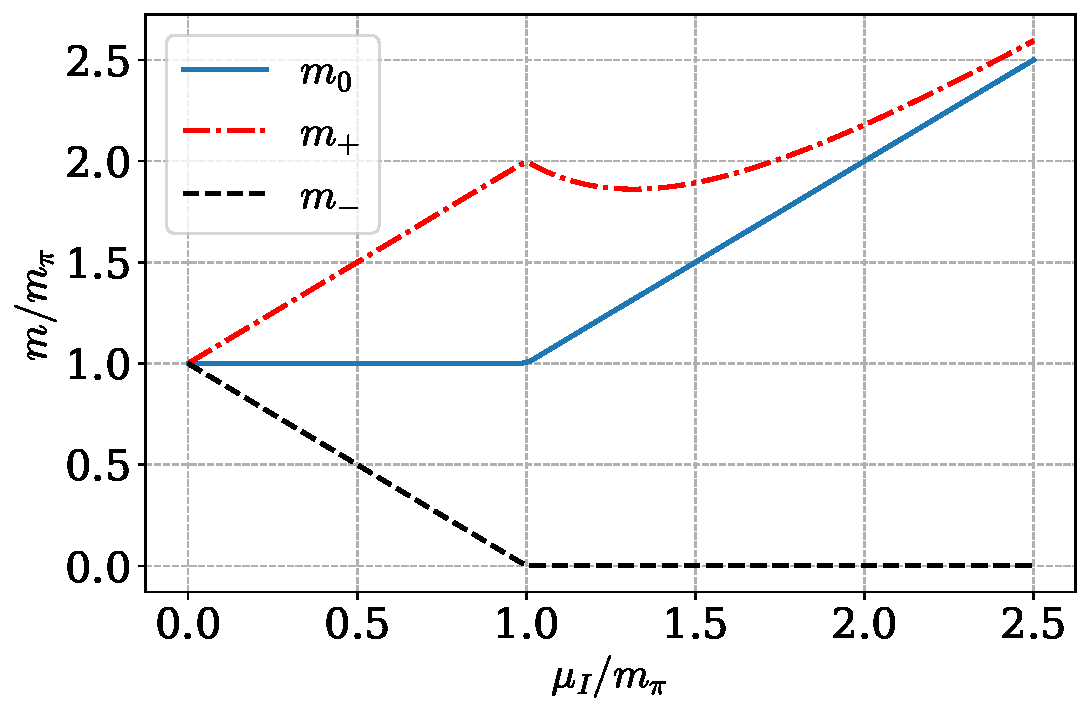
\includegraphics[width=0.7\textwidth]{../scripts/figurer/leading_order_masses.pdf}
    \caption{The masses of the three particles as functions of isosopin chemical potential. Rresults are given in units of the pion mass, $m_\pi$.}
    \label{fig: masses}
\end{figure}

With the energies of the pions, we can write the determinant of the inverse propagator as
%
\begin{equation}
    \det(D^{-1}) = (p_0^2 - E_0^2) (p_0^2 - E_+^2) (p_0^2 - E_-^2).
\end{equation}
%
The propagator and the inverse propagator in momentum space obey\footnote{One has to be careful regarding the factor $i$ in the physicist's definition of propagators. It has the consequence that $D^{-1}$ is not strictly the operator inverse of the propagator $D$.}
%
\begin{equation}
    \sum_c D_{ac}(p)D_{cb}^{-1}(p) = i \delta_{ab}
\end{equation}
%
Using this, we can solve for the propagator
%
\begin{align}
    D & = (- iD^{-1})^{-1} 
    \label{free pion propagator}
    = i
    \begin{pmatrix}
        \frac{
            p^2 - m_2^2
        }
        {
            (p_0^2 - E_+^2)(p_0^2 - E_-^2)
        } 
        & \frac{
            - ip_0m_{12}
        }
        {
            (p_0^2 - E_+^2)(p_0^2 - E_-^2)
        } & 0 \\
        \frac{
            ip_0m_{12}
        }
        {
            (p_0^2 - E_+^2)(p_0^2 - E_-^2)
        }
        & \frac{
            p^2 - m_1^2
        }
        {
            (p_0^2 - E_+^2)(p_0^2 - E_-^2)
        } & 0 \\
        0 & 0 & 
        \frac{1}{p_0^2 - E_0^2}
    \end{pmatrix}.
\end{align}




    \section{*Next-to-leading order Lagrangian}

Constructing the next-to-leading order (NLO) Lagrangian is now a business of combining the building blocks we found in \autoref{section: chiral perturbation theory}. 
We must include all terms that obey all symmetries and that are fourth-order in Weinberg's power counting scheme and remove possible redundant terms, as discussed in \autoref{appendix: rewriting terms}.
We will quote the result from \cite{schererIntroductionChiralPerturbation2002},
%
\begin{align}
    \notag
    \Ell_4 
    & = 
    \frac{l_1}{4}\Tr{\nabla_\mu \Sigma (\nabla^\mu \Sigma)^\dagger}^2
    + \frac{l_2}{4} \Tr{\nabla_\mu \Sigma (\nabla_\nu \Sigma)^\dagger} 
    \Tr{\nabla^\mu \Sigma (\nabla^\nu \Sigma)^\dagger} 
    +
    \frac{l_3 + l_4}{16} \Tr{\chi \Sigma^\dagger + \Sigma \chi^\dagger}^2
    \\ \notag
    &
    + \frac{l_4}{8}\Tr{\nabla_\mu \Sigma (\nabla^\mu \Sigma)^\dagger} \Tr{\chi \Sigma^\dagger + \Sigma \chi^\dagger}
    - \frac{l_7}{16} \Tr{\chi \Sigma^\dagger - \Sigma \chi^\dagger}^2
    + \frac{h_1 + h_3 - l_4}{4} \Tr{\chi \chi^\dagger} \\
    & +
    \frac{h_1 - h_3 - l_4}{16}
    \left[
        \Tr{\chi \Sigma^\dagger + \Sigma \chi^\dagger}^2
        + \Tr{\chi \Sigma^\dagger - \Sigma \chi^\dagger}^2
        -2 \Tr{\left(\chi \Sigma^\dagger\right)^2 + \left( \Sigma \chi^\dagger\right)^2}
    \right]
    \label{NLO Lagrangian}.
\end{align}
%
We have ignored terms containing the field strength tensors for external fields, as they vanish in our case.
The parameters $l_i$ and $h_i$ are called low energy constants, or LEO.
In \autoref{appendix: rewriting terms}, we show how to rewrite the Lagrangian to match the one used in~\autocite{adhikariTwoflavorChiralPerturbation2019,martinariaTwoflavorChiralPerturbation2020}.
To obtain $\Ell_4$ to $\Oh{\left((\pi/f)^3\right)}$, we use the result from \autoref{Sigma derivative} and \autoref{sigma commutator}, which gives
%
\begin{align*}
    %%%%%%%%%%%%%%%%%%
    % partial square %
    %%%%%%%%%%%%%%%%%%
    \Tr{\partial_\mu \Sigma \partial_\nu \Sigma^\dagger}
    & = 2 \frac{\partial_\mu \pi_a \partial_\nu \pi_a}{f^2} \\
    %%%%%%%%%%%%%%
    % Cross term %
    %%%%%%%%%%%%%
    -i \Tr{\partial_\mu \Sigma [v_\nu, \Sigma^\dagger] - \hc}
    & = 
    \frac{2\mu_I\pi_2}{f}(\delta_\mu^0\partial_\nu + \delta_\nu^0\partial_\mu)\sin{\alpha} + 
    \frac{2\mu_I}{f^2}
    [
        \pi_1 (\delta_\mu^0\partial_\nu + \delta_\nu^0\partial_\mu)\pi_2 
        - \pi_2 (\delta_\mu^0\partial_\nu + \delta_\nu^0\partial_\mu)\pi_1
    ]\cos{\alpha}
    \\
    %%%%%%%%%%%%%%%%%
    % Comm. squared %
    %%%%%%%%%%%%%%%%%
    - \Tr{[v_\nu, \Sigma] [v_\nu, \Sigma^\dagger]}
    & = 2 \mu_I{}^2 \delta_\mu^0 \delta_\nu^0 
    \left[
        \sin^2{\alpha} + \frac{\pi_1}{f} \sin{2\alpha} 
        + \frac{\pi_a \pi_b}{f^2} 
        k_{ab}
    \right],
\end{align*}
%
up to $\Oh{\left((\pi/f)^3\right)}$.
Inserting $\chi= 2 B_0 m = \bar m^2 \one + \Delta m^2 \tau_3$ gives
%
\begin{align*}
    \chi \Sigma^\dagger + \Sigma \chi^\dagger
    & = 2(\bar m^2 + \Delta m^2 \tau_3)
        \left[
            \left(
                1 
                - \frac{\pi_a^2}{2f^2}
            \right)
            \cos{\alpha}
            - \frac{\pi_1}{f}    
            \sin{\alpha}
        \right]
    \\
    &
    + 2\Delta m^2
    \left[
        \left(
            1 
            - \frac{\pi_a^2}{2f^2}
        \right)
        \tau_2 \sin{\alpha}
        +  \frac{\pi_a}{f}
        \left(
            \delta_{a1} \tau_2 \cos{\alpha} - \delta_{a2} \tau_1
        \right)
    \right], \\
    %%%%%%%%%%%%%%
    % Difference %
    %%%%%%%%%%%%%%
    \chi \Sigma^\dagger  - \Sigma \chi^\dagger
    & = -2i \bar m^2
        \left[
            \left(
                1 - \frac{\pi_a^2}{2f^2}
            \right)
            \tau_1 \sin{\alpha}
            +  \frac{\pi_a}{f}    \left(
                \tau_a 
                - 2 \delta_{1a} \tau_1 \sin^2{\frac{\alpha}{2}}
            \right)        
        \right]
        -2i \Delta m^2 \frac{\pi_3}{f}.
\end{align*}
%
Combining these results gives all the terms in $\Ell_4$, to $\Oh{\left((\pi/f)^3\right)}$:
%%%%%%%%%%%%%%%%%
% Parts for L_4 %
%%%%%%%%%%%%%%%%%
\begingroup
\allowdisplaybreaks % Make page break possible
\begin{align}
    %%%%%%%
    % l_1 %
    %%%%%%%
    \notag
    & \Tr{\nabla_\mu \Sigma (\nabla^\mu \Sigma)^\dagger}^2 
    =
    \Tr{\partial_\mu \Sigma \partial^\mu \Sigma ^\dagger
    - i \left( \partial_\mu \Sigma [v^\mu,\Sigma^\dagger] - \hc \right)
    - [v_\mu, \Sigma][v^\mu,\Sigma^\dagger]
    }^2 \\\notag
    &\quad  =
    \frac{8 \mu_I^2}{f^2} 
    (\partial_\mu \pi_a \partial^\mu \pi_a + 2 \partial_\mu \pi_2 \partial^\mu \pi_2)
    \sin^2{\alpha} \\\notag
    &\quad  + 16 \mu_I^3 \left[
        \frac{\partial_0 \pi_2}{f}
            \sin^3{\alpha}
        + \frac{1}{f^2} \left(3 \pi_1 \partial_0 \pi_2 - \pi_2 \partial_0 \pi_1\right)
            \cos{\alpha} \sin^2{\alpha}
    \right] \\ \label{l1}
    & \quad + 4 \mu_I^4 
    \left\{
        \sin^4{\alpha}
        + 2 \sin^2{\alpha}
        \left[
            \frac{\pi_1}{f}\sin{2\alpha}
            + \frac{\pi_a \pi_b}{f^2}        
            \left(k_{ab} + 2\delta_{a1}\delta_{a2}\cos^2{\alpha} \right)
        \right]
    \right\}, \\
    %%%%%%%
    % l_2 %
    %%%%%%%
    \notag
    & \Tr{\nabla_\mu \Sigma (\nabla_\nu \Sigma)^\dagger} \Tr{\nabla^\mu \Sigma (\nabla^\nu \Sigma)^\dagger}\\ \notag
    & \quad = \frac{4 \mu_I{}^2}{f^2}
    \left(
        \partial_0 \pi_a\partial_0 \pi_a + \partial_0 \pi_2\partial_0 \pi_2 + \partial_\mu \pi_2\partial^\mu \pi_2
    \right) \sin^2{\alpha} \\\notag
    &\quad  + 16 \mu_I^3 \left[
        \frac{\partial_0 \pi_2}{f}\
            \sin^3{\alpha}
        + \frac{1}{f^2} \left(3 \pi_1 \partial_0 \pi_2 - \pi_2 \partial_0 \pi_1\right)
        \cos{\alpha} \sin^2{\alpha}
    \right] \\\label{l2}
    & \quad + 4 \mu_I^4 
    \left\{
        \sin^4{\alpha}
        + 2 \sin^2{\alpha}
        \left[
            \frac{\pi_1}{f}\sin{2\alpha} 
            + \frac{\pi_a \pi_b}{f^2}        
            \left(k_{ab} + 2 \delta_{a1}\delta_{a2} \cos^2{\alpha} \right)
        \right]
    \right\}, \\
    %%%%%%%
    % l_4 %
    %%%%%%%
    \notag
    & \Tr{\nabla_\mu \Sigma (\nabla^\mu \Sigma)^\dagger} 
    \Tr{\chi \Sigma^\dagger + \Sigma \chi^\dagger } \\\label{l4}
    & \quad =
    4\bar m^2
    \Bigg\{
        2 \frac{\partial_\mu \pi_a \partial^\mu \pi_a}{f^2} \cos{\alpha}
        + 4 \mu_I 
        \left[
            \frac{\partial_0 \pi_2}{2 f} \sin{2\alpha}
            + \frac{1}{f^2}
            \left(
                \pi_1 \partial_0 \pi_2 \cos{2\alpha}
                - \pi_2 \partial_0 \pi_1\cos^2{\alpha}
            \right)
        \right]\\\notag
        & \quad + \mu_I{}^2
        \left[
            2\cos{\alpha}\sin^2{\alpha} 
            - 2 \frac{\pi_1}{f} \sin{\alpha}
            \left(2 - 3\sin^2{\alpha}\right)
            + \frac{1}{f^2}
            \left(                
                \pi_1^2[2 - 9 \sin^2{\alpha}]
                + \pi_2^2 [2 - 3 \sin^2{\alpha}]
                - 3\pi_3^2\sin^2{\alpha}
            \right)
            \cos{\alpha}
        \right]
    \Bigg\}, \\
    %%%%%%%
    % l_3 %
    %%%%%%%
    \label{l3}
    & \Tr{\chi \Sigma^\dagger + \Sigma \chi^\dagger }^2
    = 16 \bar m^4
    \left[
        \cos^2{\alpha} 
        - \frac{\pi_1}{f} \sin{2\alpha}
        + \frac{1}{f^2}\left(\pi_1^2 \sin^2{\alpha} - \pi_a \pi_a \cos^2{\alpha}\right)
    \right], \\
    %%%%%%%
    % l_7 %
    %%%%%%%
    \label{l7}
    & \Tr{\chi \Sigma^\dagger - \Sigma \chi^\dagger }^2
     = - 16 \left( \frac{\Delta m^2 \pi_3}{f} \right)^2, \\
    %%%%%%%
    % h_3 %
    %%%%%%%
    \notag
    & \Tr{\left(\chi \Sigma^\dagger\right)^2 + \left(\Sigma \chi^\dagger \right)^2}
    \\\label{h3}
    & \quad \quad = 4 \bar m^4
    \left(
        \cos{2\alpha} 
        - 2\frac{\pi_1}{f} \sin{2\alpha}
        - 2\frac{\pi_a \pi_a}{f^2} \cos^2{\alpha}
        + 2\frac{\pi_1^2}{f^2} \sin^2{\alpha}
    \right)
    + 4 \Delta m^4
    \left(
        1- 2\frac{ \pi_3^2}{f^2}
    \right)
    , \\
    %%%%%%%
    % h_2 %
    %%%%%%%
    \label{h2}
    & \Tr{\chi^\dagger \chi} = 2 {\bar m}^4 + 2{\Delta m}^4.
\end{align}
%

\endgroup

The different terms of the NLO Lagrangian is
\begingroup
\allowdisplaybreaks 
%
\begin{align}
    \Ell_4^{(0)} & =
    %
    %
    % zeroth-order
    %
    %
    (l_1 + l_2)\mu_I^4 \sin^4{\alpha}
    + (l_3 + l_4)\bar m^2 \cos^2{\alpha}
    + l_4 \bar m \mu_I{}^2 \cos{\alpha} \sin^2{\alpha}
    + (h_1 - l_4)\bar m^4
    + h_3 \Delta m^4,
    \label{NLO-L0}
    \\
    %
    %
    % first order
    %
    %
    \nonumber
    \Ell_4^{(1)} & =
    4 \mu_I^3 \frac{l_1 + l_2}{f}
    \left(
        \partial_0 \pi_2 
        % term 5 pi
        + \mu_I 
        \cos{\alpha} \pi_1
    \right)\sin^3{\alpha}
    % term 13 pi
    -
    \frac{l_3 + l_4}{f}
    \bar m^4
    \pi_1 \sin{2\alpha}
    %%%%%%%% 
    \\ \label{NLO-L1}
    & 
    +
    \bar m^2
    \frac{l_4}{f}
    \left[
        % term 16 pi
        \mu_I 
        \partial_0 \pi_2 \sin{2\alpha}
        - \mu_I{}^2
        % term 19 pi
        \pi_1 \sin{\alpha}
        \left(3\sin^2{\alpha} - 2\right)
    \right],
    \\
    %
    %
    % second order
    %
    %
    \nonumber
    \Ell_4^{(2)} & = 
    2 \mu_I^2 \frac{l_1}{f^2}
    ( 
        \partial_\mu \pi_a \partial^\mu \pi_a
        + 2 \partial_0 \pi_2 \partial_0 \pi_2    
    )
        \sin^2{\alpha}
    + \mu_I{}^2 
    \frac{ l_2}{f^2}
    % term 7 pi^2
    \left(
        \partial_\mu \pi_2 \partial^\mu \pi_2
        + 2\partial_0 \pi_a\partial_0 \pi_a 
        + 2\partial_0 \pi_2 \partial_0 \pi_2
    \right) 
    \sin^2{\alpha}
    \\ \nonumber
    & + 
    2 \frac{l_1 + l_2}{f^2}
    \left[
        % term 3 pi^2
        2\mu_I^3 
        \left( 3 \pi_1 \partial_0 \pi_2 - \pi_2 \partial_0 \pi_1 \right)
        \cos{\alpha}
        % term 6 pi^2
        + \mu_I^4  \pi_a \pi_b 
            \left(k_{ab} + 2\delta_{a1}\delta_{a2}\cos^2{\alpha} \right)
    \right]\sin^2{\alpha}
    % 
    \\ \nonumber
    & +
    \frac{l_3 + l_4}{f^2}
    \bar m^2
    % term 14 pi^2
    \left(\pi_1^2 \sin^2{\alpha} - \pi_a \pi_a \cos^2{\alpha}\right)
    +  \frac{l_4}{f^2}
    \bar m^2
    \bigg[
    % term 15 pi^2
    \partial_\mu \pi_a \partial^\mu \pi_a \cos{\alpha}
    + 4 \mu_I 
    % term 17 pi^2
    \left(
        \pi_1 \partial_0 \pi_2 \cos{2\alpha}
        - \pi_2 \partial_0 \pi_1\cos^2{\alpha}
    \right)
    \\
    & %\hspace{55 pt}
    +\frac{1}{2} \mu_I{}^2
    % term 20 pi^2
    \left(                
        \pi_1^2[2 - 9 \sin^2{\alpha}]
        + \pi_2^2 [2 - 3 \sin^2{\alpha}]
        - 3\pi_3^2\sin^2{\alpha}
    \right)
    \cos{\alpha}
    \bigg]
    % \\ 
    % &
    % term 21 pi^2
    + \frac{l_7}{f^2}
    \Delta m^2 \pi_3^2.
    \label{NLO-L2}
\end{align}
%
\endgroup


    \section{Three-flavor \chpt\ to leading order}
\label{section: three-flavor chpt to leading order}


Using the building blocks from last section, we can build the leading order Lagrangian, which is~\autocite{eckerRoleResonancesChiral1989,gasserChiralPerturbationTheory1984,gasserChiralPerturbationTheory1985,schererIntroductionChiralPerturbation2002}
%
\begin{equation}
    \label{leading order three-flavor Lagrangian}
    \Ell_2 
    = \frac{1}{4}f^2 \Tr{\nabla_\mu \Sigma \nabla^\mu \Sigma^\dagger}
    + \frac{1}{4}f^2 \Tr{\chi \Sigma^\dagger + \Sigma \chi^\dagger}
    + e^2 C \Tr{\Sigma Q \Sigma^\dagger Q}.
\end{equation}
%
We will work with three flavors, i.e. $N_f = 3$, so the mass matrix is now
%
\begin{equation}
    m = 
    \begin{pmatrix}
        m_u & 0 & 0 \\
        0 & m_d & 0 \\
        0 & 0 & m_s
    \end{pmatrix}.
\end{equation}
%
When we evaluate $s = m$ and $p = 0$, the scalar term then becomes
%
\begin{equation}
    \chi = 2B_0 m = 
    \begin{pmatrix}
        \bar m^2 - \Delta m^2 & 0 &0\\
        0& \bar m^2 + \Delta m^2 & 0 \\
        0&0&m_S^2
    \end{pmatrix},
\end{equation}
%
where we have defined
%
\begin{equation}
    \bar m^2 =  B_0(m_u + m_d),\quad 
    \Delta m^2 = B_0(m_d - m_u), \quad
    m_S^2 = 2B_0 m_s.
\end{equation}
%
The charge matrix is
%
\begin{equation}
    \label{three-flavor charge matrix}
    Q = \frac{1}{3}
    \begin{pmatrix}
        2 & 0 & 0\\
        0 & -1 & 0\\
        0 & 0 & -1
    \end{pmatrix}
    = \frac{1}{2} \left( \lambda_3 + \frac{1}{\sqrt{3}} \lambda_8 \right).
\end{equation}
%
In the vacuum, when there are no external currents, we choose the standard, exponential parametrization of the Goldstone manifold,
%
\begin{equation}
    \Sigma(x) = \exp{i\frac{\varphi_a \lambda_a}{f}}.
\end{equation}
%
Here, $\lambda_\alpha$ are the Gell-Mann matrices, as shown in \autoref{section: algebra bases}, are generators of $\Lie{SU}{3}$, and $f$ is the bare pion decay constant.
There are eight Goldstone bosons, $\varphi_a$, which are real functions of space-time.
This parametrization ensures that $\varphi = 0$ corresponds to the vacuum.
Using the isospin transformation rule \autoref{sigma transform under H}, we can perform an infinitesimal transformation of the Goldstone fields,
%
\begin{equation}
    \Sigma \rightarrow U_V \Sigma U_V^\dagger
    \sim
    \left(1 + i \eta_a \frac{1}{2} \lambda_a\right)
    \left(1 + i \frac{1}{f} \varphi_b  \lambda_b\right)
    \left(1 - i \eta_c \frac{1}{2} \lambda_c\right)
    \sim
    1 + i\frac{\varphi_a}{f} \lambda_a + i \frac{\varphi_a}{f} \eta_b f_{abc} \lambda_c,
\end{equation}
%
or
%
\begin{equation}
    \varphi_a \rightarrow [\delta_{ab} + i\eta_\alpha (-if_{\alpha ab})] \varphi_b.
\end{equation}
%
That is, $\varphi_a$ transforms under the adjoint representation of $\lie{su}{3}$, which is made up of elements of the form $\eta_\alpha (-i f_{\alpha ab})$.
The $\lie{su}{3}$ Lie algebra has three independent $\lie{su}{2}$ sub-algebras.
We introduce the matrices
%
\begin{equation}
    \lambda_Q = \lambda_3 + \frac{1}{\sqrt{3}}\lambda_8, \quad
    \lambda_K = -\lambda_3 + \frac{1}{\sqrt{3}}\lambda_8,
\end{equation}
%
From the structure constants, \autoref{structure constants su(3)}, we can conclude that they commute, i.e., $[\lambda_Q, \lambda_K] = 0$.
Furthermore, we find the commutation relations
%
\begin{equation}
    [\lambda_i, \lambda_j] = 2i \epsilon_{ijk} \lambda_k,\quad
    ijk \in \{1, 2, 3\}, \, \{4, 5, Q\}, \, \text{or} \, \{6, 7, K\}.
\end{equation}
%
We here define the Levi-Civita symbol by $\epsilon_{123} = \epsilon_{34Q} =\epsilon_{67K} = 1$.
This is the defining commutation relation of $\lie{su}{2}$.
The first subalgebra, spanned by $\{ \lambda_1, \lambda_2, \lambda_3 \}$, corresponds to isospin transformations, which are rotations of the up and down quark into each other.
Consider the transformation where $\eta_3 \neq 0$, while $\eta_\alpha = 0$ for $\alpha \neq 3$.
Acting on the quarks, this transformation is generated by $\lambda_3$, while in the adjoint representation the generator is $f_{3ab}$.
Under this transformation,  $\varphi_3\lambda_3$ is invariant.
We can see this from the fact that the structure constants $f_{abc}$ is totally antisymmetric, and thus $f_{33b} = 0$.
This means that $\varphi_3$ has the quantum number $I_3 = 0$.
$\varphi_1\lambda_1$ and $\varphi_2\lambda_2$ do not have definite values of the third component of isospin as they are not eigenvectors of $f_{3ab}$, but they do have definite values for the first and second component.
The linear combinations $\pi^\pm \, (\lambda_1 \mp \lambda_2)$, on the other hand, do.
This shows the relationship between our fields $\varphi_a$, and the observed, charged pions $\pi^+$ and $\pi^-$, as they have definite values for $I_3$.\footnote{
    Authors differ if they define $\sqrt 2 \pi^\pm = \varphi_1 \pm i \varphi_2$, or with opposite signs, $\sqrt 2 \pi^\pm = \varphi_1 \mp i \varphi_2$.  We choose the latter, so that $\pi_+ \ket{0}$ is the state with the quantum numbers of the positive pion.
    }
The full relationship between the $\varphi_a$-fields  and the observed pseudoscalar mesons is~\autocite{schererIntroductionChiralPerturbation2002}
%
\begin{equation}
    \varphi_a \lambda_a
    =
    \begin{pmatrix}
        \varphi_3 + \frac{1}{\sqrt{3}} \varphi_8 & \varphi_1 - i \varphi_2 & \varphi_4 - i \varphi_5 \\
        \varphi_1 + i \varphi_2 & \varphi_3 + \frac{1}{\sqrt{3}} \varphi_8 & \varphi_6 - i \varphi_7  \\
        \varphi_4 - i \varphi_5 & \varphi_6 - i \varphi_7  & \frac{2}{\sqrt{3}} \varphi_8
    \end{pmatrix}
    =
    \begin{pmatrix}
        \pi_0 + \frac{1}{\sqrt{3}}\eta & \sqrt{2}\pi^+ & \sqrt{2}K^+ \\
        \sqrt{2}\pi^- & -\pi_0 + \frac{1}{\sqrt{3}}\eta & \sqrt{2}K^0 \\
        \sqrt{2}K^- & \sqrt{2}\bar K^0  & - \frac{2}{\sqrt 3} \eta
    \end{pmatrix}.
\end{equation}




\subsection{Ground state}

When we take into account chemical potentials, we need to pick a new parametrization.
We will start the analysis by assuming $e = 0$ and then reintroduce electromagnetic interactions later.
The covariant derivative is then
%
\begin{equation}
    \nabla_\mu \Sigma = \partial_\mu \Sigma - i [v_\mu, \Sigma], \quad 
    v_\mu = \mu \delta^0_\mu.
\end{equation}
%
The chemical potential matrix $\mu$ has three independent degrees of freedom for each quark, an is of the form
%
\begin{equation}
    \mu = 
    \begin{pmatrix}
        \mu_u & 0 & 0 \\
        0 & \mu_d & 0 \\
        0 & 0 & \mu_s
    \end{pmatrix}
    = 
    \begin{pmatrix}
        \frac{1}{3}\mu_B + \frac{1}{2}\mu_I & 0 & 0 \\
        0 & \frac{1}{3}\mu_B - \frac{1}{2}\mu_I & 0 \\
        0 & 0 & \frac{1}{3}\mu_B - \mu_S
    \end{pmatrix}
    = \frac{1}{3}(\mu_B - \mu_S) \one 
    + \frac{1}{2} \mu_I \lambda_3
    + \frac{1}{\sqrt{3}}\mu_S\lambda_8,
\end{equation}
%
where we have defined $\mu_B = \frac{3}{2}(\mu_u + \mu_d)$, $\mu_I = \mu_u - \mu_d $ and $\mu_S = \frac{1}{2}(\mu_u + \mu_d)-\mu_s$.
Here, $\mu_u$, $\mu_d$, and $\mu_s$ are the up, down, and strange quark chemical potentials, while $\mu_B$, $\mu_I$, and $\mu_S$ are the baryon number, isospin, and strangeness chemical potentials.
$\Sigma$ transforms as $\Sigma \rightarrow \Sigma$ under $U(1)_V$, the symmetry corresponding to the baryon number; it is a baryon number singlet.
This reflects the fact that the baryon number of mesons, and thus the $\varphi_a$'s, is zero.
Therefore, the chemical potential corresponding to the baryon number, $\mu_B$, should not affect the final result.
We can also see this because $\mu_B$ only appears with the identity matrix $\one$ in $\mu$.
Any dependence on $\mu_B$ in $\nabla_\mu \Sigma$ will vanish as $\one$ commutes with everything.

We will assume the ground state is a spatially independent configuration, $\varphi_a^0 =\const$
This configuration must then minimize the free energy, too leading order, is equivalent to minimizing the static Hamiltonian, i.e., $\He^{(0)} = \He[\varphi^0]$.
To this end, we define
%
\begin{equation}
    \Sigma_\alpha 
    = \exp{i \alpha n_a \lambda_a},
    \quad \alpha = \frac{1}{f} \sqrt{\varphi_a^0 \varphi_a^0}, \quad n_a = \frac{\varphi_a^0}{\sqrt{\varphi_b^0 \varphi_b^0}}. 
\end{equation}
%
We show how to derive the correct parametrization of the ground state in the case of two flavors in \autoref{section: leading order}.
For $\mu_S = 0$, we expect to recover this result, in which $n_1^2 + n_2^2 =1$, and thus $n_a = 0$ for $a>2$.
Furthermore, we showed that we may choose $n_1 = 0$ without loss of generality, in which case the ground state becomes
%
\begin{equation}
    \Sigma_\alpha^{\pipm} = \exp{i \alpha \lambda_2} = (\one - \lambda^2_2) + \lambda_2^2 \cos\alpha + i \lambda_2\sin\alpha.
\end{equation}
%
The ground state is thus parameterized by $\alpha$ only.
As we will show in \autoref{chapter: thermodynamics}, when the isospin chemical potential exedes a critical value, $\mu_I \geq \mu_I^c$, the system undergoes a phase transition from the vacuum phase to a phase in which $\alpha \neq 0$, and the charged pions form a condensate.
It is only when we reach this phase that the equation of state is non-trivial at $T=0$, which makes it possible for pion stars to form.

If we define $\mu_\Kpm = \mu_S + \frac{1}{2}\mu_I$ and $\mu_\Ko = \mu_S - \frac{1}{2}\mu_I$, then we can write the terms of the QCD Lagrangian made up of $\mu_I$ and $\mu_S$ and their corresponding currents densities as
%
\begin{equation}
    \bar q \gamma^0\left(\frac{1}{2}\mu_I \lambda_3 + \frac{1}{\sqrt 3}\mu_S \lambda_8 \right) q
    = 
    \bar q\gamma^0 \left( \frac{1}{2}\mu_\Kpm \lambda_Q + \frac{1}{2} \mu_\Ko \lambda_K\right) q.
\end{equation}
%
Analogously to how a higher $\mu_I$ leads to a condensate in the first $\lie{su}{2}$ subalgebra, we can expect these chemical potentials to lead to different condensates in their respective subalgebras.
If we assume $\mu_\Ko = 0$, we would expect the new ground state to take the form
%
\begin{align}
    \Sigma_\alpha^{\Kpm} = \exp{i \alpha \lambda_5} = (\one - \lambda^2_5) + \lambda_5^2 \cos\alpha + i \lambda_5\sin\alpha.
\end{align}
%
This analysis extends to all four quadrants of the $\mu_I-\mu_S$ plane.
If we set $\mu_\Kpm = 0$, we would expect a ground state of the form $e^{i\alpha\lambda_7}$.
In \autocite{kogutQCDSmallNonzero2001}, \citeauthor{kogutQCDSmallNonzero2001} show that this analysis is right, and that these states are local minima of the static Lagrangian.
However, the domains of the different condensates overlap, so there is a phase transition between the condensates.
We will study the different condensates and the transition between them in \autoref{chapter: thermodynamics}.



\subsection{The pion-condensed phase}

Similar to what we found for the two-flavor case in \autoref{section: two-flavor chpt to leading order}, the ground states of the different condensates are parameterized as
%
\begin{equation}
    \Sigma(x) = A^i_\alpha U(x) \Sigma_0 U(x) A^i_\alpha, \quad
    U(x) = \exp{i \frac{\varphi_a \lambda_a}{2 f}}, \quad
    A_\alpha^i = \exp{i \frac{\alpha \lambda_i}{2}},
\end{equation}
%
where $i = 2, 5, 7$ depending on which phase we are in.
We start working in the pion-condensed phase, so $i = 2$, and assume $\mu_I > 0$ and $e = 0$.
Inserting this into \autoref{leading order three-flavor Lagrangian}, and expanding up to and including $\Oh\left((\pi/f)^2\right)$, we get
%
\begin{align}
    \label{static three-flavor Lagrangian}
    \Ell_2^{(0)} 
    &=
    \frac{1}{2} f^2
    \left(
        \mu_I^2 \sin^2\alpha
        + 2\bar m \cos\alpha
        + m_S
    \right), \\
    \label{linear three-flavor Lagrangian}
    \Ell_2^{(1)}
    &=
    -f \mu_I \partial_0 \varphi_1 \sin\alpha
    + f \sin\alpha
    \left(
        \mu_I^2\cos\alpha - \bar m^2
    \right)\varphi_2, \\
    \label{quadratic three-flavor Lagrangian}
    \Ell_2^{(2)} 
    &= 
    \frac{1}{2}\partial_\mu \varphi_a \partial^\mu \varphi_a
    + \frac{1}{2} m_{ab} \varphi_a\partial_0\varphi_b
    - \frac{1}{2} m_a^2 \varphi_a^2
    - \frac{1}{\sqrt{3}} \Delta m^2 \varphi_3 \varphi_8.
\end{align}
%
Here, we have introduced a number of mass parameters, which will in general be functions of $\alpha$ and the chemical potentials.
The diagonal mass terms are
%
\begingroup
\allowdisplaybreaks
\begin{align}
    m_1^2 &=  \bar m^2\cos\alpha - \mu_I^2 \cos^2\alpha,\\
    m_2^2 &= \bar m^2\cos\alpha - \mu_I^2 \cos2\alpha, \\
    m_3^2 &= \bar m^2\cos\alpha + \mu_I^2 \sin^2\alpha, \\
    m_4^2 &= m_5^2 = m_-^2 - m_{\mu+}^2, \\
    m_6^2 &= m_7^2 = m_+^2 - m^2_{\mu-}, \\
    m_8^2 &= \frac{1}{3} (\bar m^2 \cos\alpha + 2 m_S^2),
\end{align}
\endgroup
%
where
%
\begin{equation}
    m_\pm^2 = \frac{1}{2} (\bar m^2 \cos\alpha \pm \Delta m^2 + m_S^2),
    \quad
    m^2_{\mu\pm } = \frac{1}{4}\mu_I^2 \cos2\alpha \pm \mu_I\mu_S \cos\alpha + \mu_S^2.
\end{equation}
%
At $\mu_S = \mu_I = 0$ and $\alpha = 0$, these correspond to the well known leading-order masses of the pseudoscalar mesons~\autocite{eckerChiralPerturbationTheory1995},
%
\begin{align}
    \label{leading order pion mass mu=0}
    m_1^2 & = m_2^2 = m_3^2 
    = \bar m^2 
    = B_0(m_u + m_d) = m_\pi^2, \\
    \label{leading order charged kaon mass mu=0}
    m_4^2 & = m_5^2 
    = \frac{1}{2} (\bar m^2 - \Delta m^2 + m_S^2) 
    = B_0(m_u + m_s) = m_{\Kpm}^2, \\
    \label{leading order neutral kaon mass mu=0}
    m_6^2 &= m_7^2 
    = \frac{1}{2} (\bar m^2 + \Delta m^2 + m_S^2) 
    = B_0(m_d + m_s) = m_{\Ko }^2, \\
    \label{leading order eta mass mu=0}
    m_8^2 
    &= \frac{1}{3}(\bar m^2  + 2m_S^2) 
    = \frac{1}{3}B_0(m_u + m_d + 4m_s) = m_\eta^2 .
\end{align}
%
In addition, we have off-diagonal terms,
%
\begin{align}
    m_{12} & = 2 \mu_I\cos\alpha,\\
    m_{45} & =\mu_I\cos\alpha + 2\mu_S, \\
    m_{76} & = \mu_I\cos\alpha - 2\mu_S.
\end{align}
%
Here, $m_{ab} = -m_{ba}$, and terms not defined above are zero.
These terms mean that the basis $\varphi_a$ does not correspond to mass eigenstates.
This is to be expected, as they are not eigenstates of isospin nor strangeness.
To find the physical masses, we must analyze the propagator and the spectrum of the theory.
We follow~\autocite{adhikariTwoflavorChiralPerturbation2019,adhikariQuarkPionAxial2021a}.
The spectrum is given by the zero of the inverse propagator, which in momentum space is
%
\begin{align}
    \nonumber
    D_{ab}^{-1} 
    &= \fdv{S}{\pi_a,\pi_b}
    =
    (p^2 - m_a^2)\delta_{ab} - i p_0 m_{ab}\\
    &= 
    \begin{pmatrix}
        p^2 - m_1^2 & -ip_0 m_{12} &&&&&&\\
        ip_0 m_{12} & p^2 - m_1^2 &&&&&0&\\
        &&p^2 - m_3^2&&&&&\\
        &&&p^2 - m_4^2&-ip_0 m_{45}&&&\\
        &&&ip_0 m_{45}&p^2 - m_5^2&&&\\
        &&&&&p^2 - m_6^2&-ip_0 m_{67}&\\
        &0&&&&ip_0 m_{67}&p^2 - m_7^2&\\
        &&&&&&&p^2 - m_8^2
    \end{pmatrix}.
\end{align}
%
We have chosen to neglect the $\pi^0 - \eta$-mixing terms $D_{83}^{-1} = D_{38}^{-1} = - \Delta m^2 / \sqrt{3}$.
We will, however, keep $\Delta m \neq 0$ in the other mass contribution.
The spectrum of the theory is given by the zeros of the determinant of the propagator,
\begin{align}
    \nonumber
    \det\left(D^{-1}\right)
    =&\,
    (p^2 - m_3^2)(p^2 - m_8^2)
    \left[ (p^2 - m_1^2)(p^2 - m_2^2) + p_0^2m_{12}^2  \right]\\
    &\times
    \left[ (p^2 - m_4^2)(p^2 - m_5^2) + p_0^2m_{45}^2  \right]\left[ (p^2 - m_6^2)(p^2 - m_7^2) + p_0^2m_{67}^2  \right]
    = 0.
\end{align}
%
Solving $\det(D^{-1}) = 0$ for $p_0^2$ gives eight roots $E_i^2$, one for each particle.
Writing the four-momentum as $p^\mu = (p_0, \vv p)$, these zeros are
%
\begingroup
\allowdisplaybreaks
\begin{align}
    E_0^2 &= |\vv p |^2 + m_3^2, \\
    E_\eta^2 &= |\vv p |^2 + m_8^2, \\
    E_\pipm^2
    & = |\vv p|^2 +
    \frac{1}{2}
    \left(
        m_1^2 + m_2^2 + m_{12}^2 
    \right)
    \mp
    \frac{1}{2}
    \sqrt{
        4|\vv p|^2m_{12}^2 
        +
        \left(
            m_1^2 + m_2^2 + m_{12}^2
        \right)^2
        - 4 m_1^2 m_2^2
    }, \\
    E_\Kpm^2
    & = |\vv p|^2 + m_4^2 + \frac{1}{2} m_{45}^2 
    \mp
    \frac{1}{2} m_{45} \sqrt{4|\vv p|^2 + 4 m_4^2 + m_{45}^2},\\
    E_\Ko^2
    &= |\vv p|^2 + m_6^2 + \frac{1}{2} m_{67}^2 
    \pm
    \frac{1}{2} m_{67} \sqrt{4|\vv p|^2 + 4 m_6^2 + m_{67}^2}.
\end{align}
\endgroup
%
The masses of the particles are given by the energy at $\vv p = 0$.
For $\alpha = 0$, which we will later show this is valid for low $\mu$'s, we get a Zeeman-like splitting of the energies of the pions,
%
\begin{equation}
    E_0^2 =\sqrt{|\vv p|^2 + \bar m^2}, \quad
    E_\pipm = \sqrt{|\vv p|^2 + \bar m^2} \mp \mu_I.
\end{equation}
%
The kaons have a similar splitting, only due to the kaon chemical potentials $\mu_\Kpm$ and $\mu_\Ko$ instead.
The masses of the various mesons are shown in \autoref{fig: leading order masses mesons}.
These results use the relationship between $\mu_I$ and $\alpha$, which we derive in next chapter.
In the lower plot, we see the Zeeman splitting of the pion masses, which persists until the mass of the positive pion vanishes.
As we explore further in next chapter, this happens as the exact isospin symmetry $\Lie{U}{1}_{I_3} \subset \Lie{SU}{3}_V $ is broken spontaneously by the pion condensate, and $\pi^+$ is the corresponding Goldstone boson.
On the top, we see that the kaons also get this Zeeman splitting in the vacuum phase.
%
\begin{figure}
    \centering
    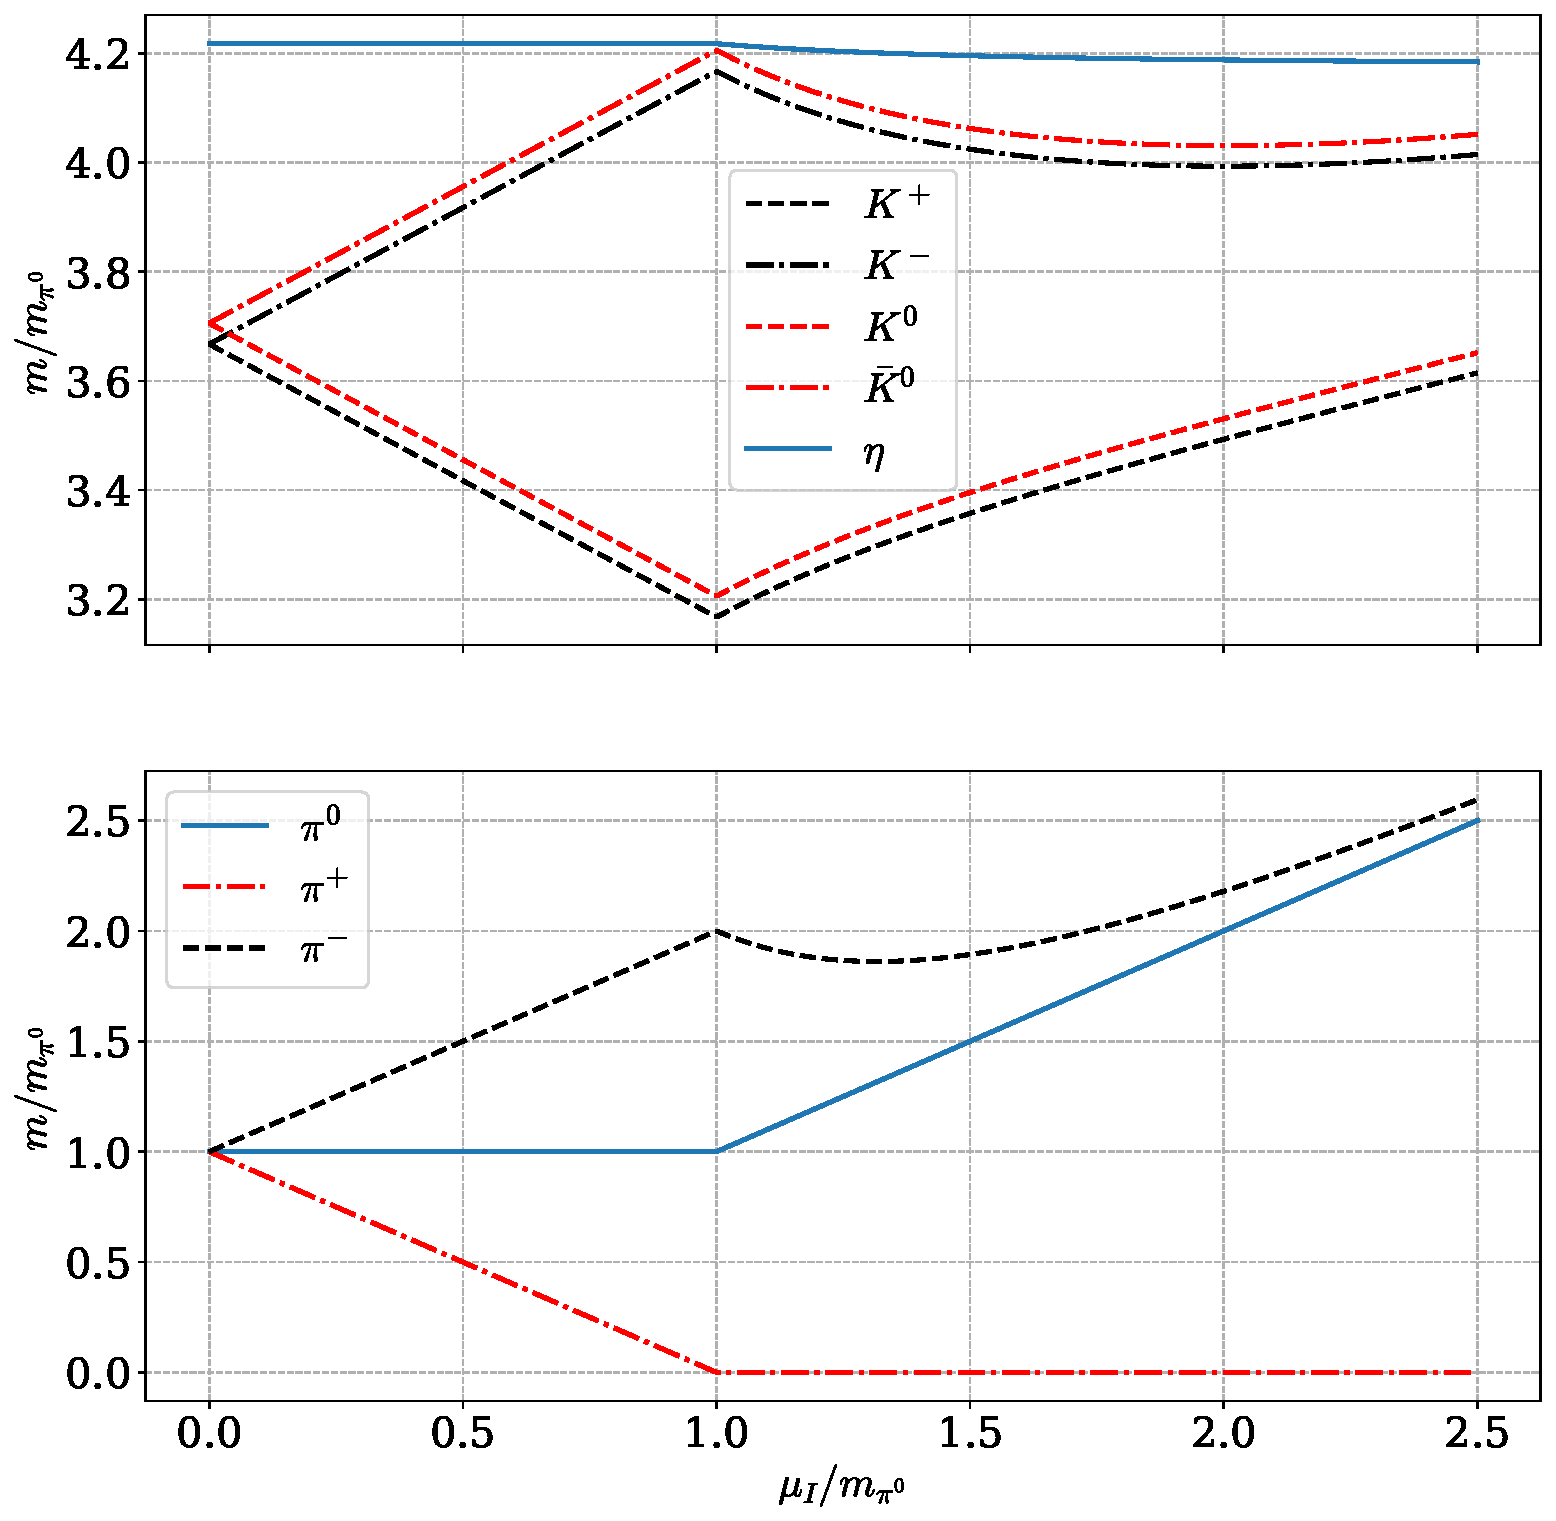
\includegraphics[width=0.6\textwidth]{../scripts/figurer/masses_mesons.pdf}
    \caption{
        The leading order masses of the pseudoscalar mesons, as functions of the isospin chemical potential.
        Both the masses and chemical potential are normalized to the pion mass.
        These results are at $\mu_S = 0$.
        The difference between the kaons at $\mu_I = 0$ is a result of the fact that $\Delta m \neq 0$.
        }
    \label{fig: leading order masses mesons}
\end{figure}
%

If we adjust the strangeness chemical potential instead, while the isospin chemical potential remains constant, then the kaons will get a similar splitting, as shown in \autoref{fig: leading order masses kaos afo strangeness}, while the pions are unaffected.
For $\mu_I > 0$, the mass of the positive kaon will reach zero first, at the point of transition into the charged kaon condensate.
At this point, the results obtained in this section will become invalid, as $\Sigma = \exp{i \alpha \lambda_2}$ no longer is the ground state.


\begin{figure}
    \centering
    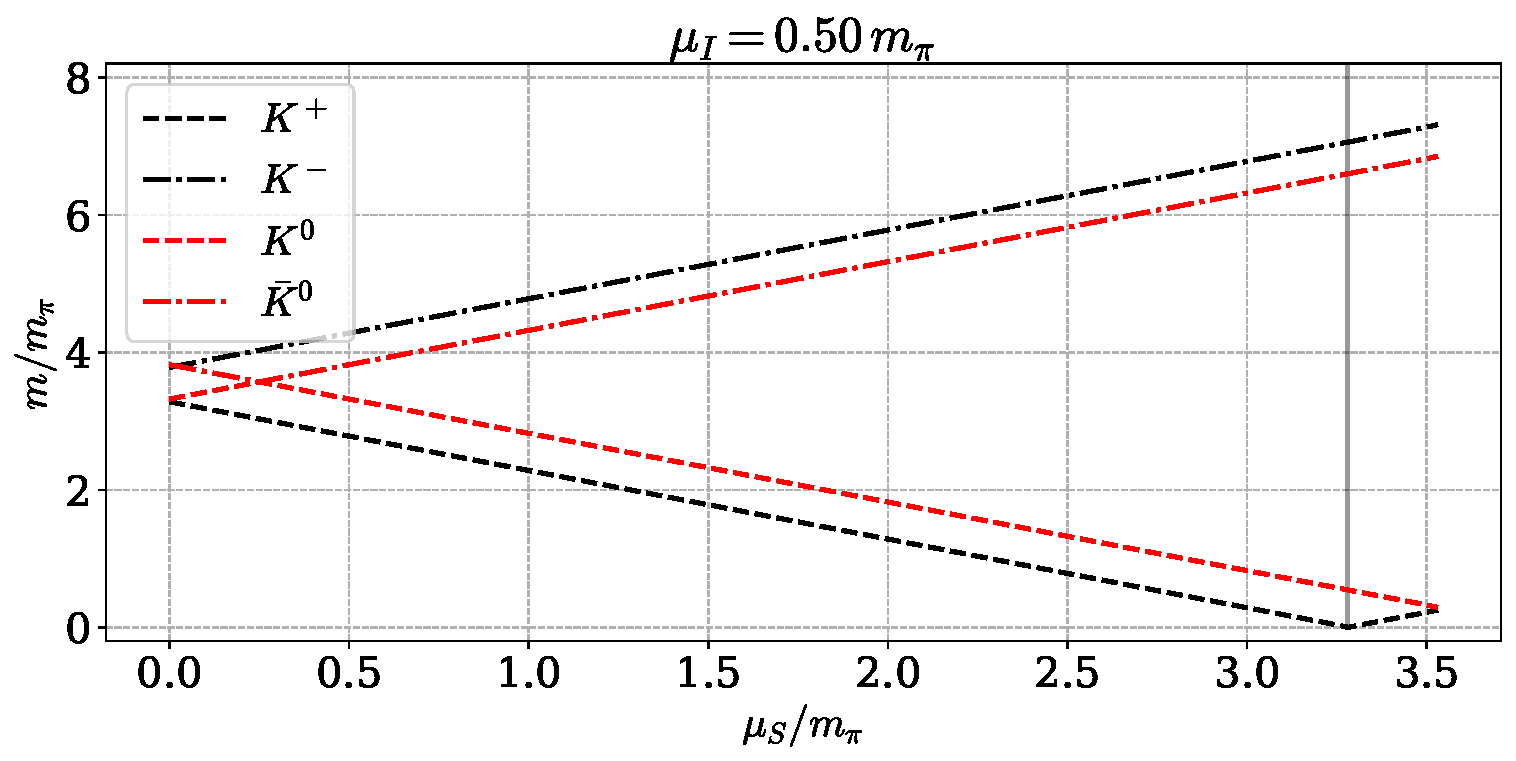
\includegraphics[width=0.8\textwidth]{../scripts/figurer/masses_kaons2.pdf}
    \caption{
        The kaon masses as a function of $\mu_S$, both in units of $m_\pi$, evaluated at $\mu_I = 0.5 \, m_\pi$.
        These results are only valid to the left of the gray line at $\mu_S\approx 3.3 \, m_\pi$, where $m_{K^+}$ reaches zero.
    }
    \label{fig: leading order masses kaos afo strangeness}
\end{figure}





\subsection{The kaon condensed phase}

In the $K^\pm$-condensate, we get
%
\begin{align}
    \label{static three-flavor Lagrangian kaon condensate}
    \Ell^{(0)}_2 
    & =
    \frac{1}{2}f^2 
    \left(
        \mu_\Kpm^2 \sin^2\alpha
        + 2m^2_\Kpm \cos\alpha
        + \bar m^2 +\Delta m^2
    \right), \\
    \label{linear three-flavor Lagrangian kaon condensate}
    \Ell_2^{(1)}
    & 
    =
    - \frac{1}{2}f\mu_\Kpm\partial_0\varphi_4 \, \sin\alpha 
    + f\sin\alpha
    \left(
        \mu_\Kpm^2 \cos\alpha
        -m_\Kpm^2
    \right)\varphi_5\\
    \label{quadratic three-flavor Lagrangian kaon condensate}
    \Ell_2^{(1)}
    & =
    \frac{1}{2} \partial_\mu \varphi_a \partial^\mu \varphi_a
    + \frac{1}{2}m'_{ab} \varphi_a\partial_0\varphi_a
    - \frac{1}{2}m'^2_{a} \varphi_a^2
    - \frac{1}{2}\Delta_{\varphi\eta} \varphi_3\varphi_8
\end{align}
%
where
\todo[]{Sjekk disse}
%
\begingroup
\allowdisplaybreaks
\begin{align}
    {m'}_{12} &= \frac{1}{2}(\cos\alpha + 3)\mu_I + (\cos\alpha - 1)\mu_S \\
    {m'}_{45} &= 2\mu_\Kpm\cos\alpha \\
    {m'}_{76} &= \frac{1}{2}(3-\cos\alpha) \mu_I - (1 + \cos\alpha)\mu_S, \\
    {m'}_1^2 & = m_2^2 = {m'}_-^2 + {m'}_{\mu-}^2\\
    {m'}_3^2 
    & = 
    \frac{1}{4}
    \left(
        \mu_\Kpm^2 \sin^2\alpha
        + \bar m^2(\cos\alpha + 3)
        + \Delta m^2 (\cos\alpha -1)
        + m_S^2(\cos\alpha - 1)
    \right)\\
    {m'}_4^2 & = m_\Kpm^2\cos\alpha -\mu_\Kpm \cos^2\alpha \\
    {m'}_5^2 & = m_\Kpm^2\cos\alpha -\mu_\Kpm \cos 2\alpha \\
    {m'}_6^2 & = m_7^2 = {m'}_+^2 + {m'}_{\mu+}^2\\
    {m'}_8^2
    & =
    \frac{1}{12}
    \left[
        \frac{9}{4}\mu_\Kpm^2\sin^2\alpha
        + \bar m^2(5\cos\alpha-1) 
        + 5\Delta m^2(\cos\alpha-1)
        + m_S^2(5\cos\alpha+3))
    \right] \\
    \Delta_{\eta\pi}
    & =
    \frac{\sqrt{3}}{2}
    \left[
        \mu_\Kpm^2\sin^2\alpha
        + \frac{1}{3}\bar m^2(\cos\alpha - 1)
        + \frac{1}{3}\Delta m^2(\cos\alpha + 3)
        + \frac{1}{3}m^2_S(\cos\alpha - 1)
    \right],
\end{align}
\endgroup
%
and
%
\begingroup
\allowdisplaybreaks
\begin{align}
    {m'}_\pm^2
    & =
    \frac{1}{4}\bar m^2 (\cos\alpha \mp 1 + 2)
    + \frac{1}{4} \Delta m^2 (\cos\alpha \mp 1-2)
    +\frac{1}{4} m_S^2 (\cos\alpha \pm 1), \\
    {m'}_{\mu\pm}^2
    & =
    \frac{1}{2}(\sin^2\alpha  \pm 3\cos\alpha - 5)\mu_I^2
    +(\sin^2\alpha\pm\cos\alpha + 1)\mu_I\mu_s
    +(\sin^2\alpha\mp\cos\alpha - 1)\mu_s^2.
\end{align}
\endgroup
%
We see that both the Lagrangian and the masses have a similar structure to the pion condensate, only with $\varphi_4$ and $\varphi_5$ taking the roles of $\varphi_1$ and $\varphi_2$, and $\mu_\Kpm$ and $m_\Kpm$ the roles of $\mu_I$ and $\bar m$.
The phase with a $\Ko$-condensate, with the ground state $\Sigma = \exp{i \lambda_7 \alpha}$ has a very similar structure.
The static Lagrangian is
%
\begin{equation}
    \label{static Lagrangian neutral kaon}
    \Ell_2^{(0)} = \frac{1}{2}f^2 
    \left(
        \mu_\Ko^2 \sin^2\alpha
        + 2m_\Ko^2\cos\alpha + \bar m^2 - \Delta m^2
    \right).
\end{equation}
%


 
\subsection{Electromagnetic contributions}

We now reintroduce $e$.
First, we set $\mu_I = \mu_S = 0$, so we are in the vacuum phase, $\Sigma = U^2 = \exp{i \varphi_a \lambda_a/f}$, and the covariant derivative is
%
\begin{equation}
    \nabla_\mu \Sigma = \partial_\mu \Sigma - i e \mathcal A_\mu [Q, \Sigma],
\end{equation}
%
where $Q$ is the charge matrix \autoref{three-flavor charge matrix}.
Inserting this into the terms of the leading-order Lagrangian, \autoref{leading order three-flavor Lagrangian}, and expanding to and including $\Oh\left((\pi/f)^2\right)$ yields
%
\begin{align}
    \nonumber
    \Ell_2
    &= 
    \frac{1}{2} \partial_\mu \varphi_a \partial^\mu \varphi_a
    - \frac{1}{2}(m_{a}^2 + \Delta m_{\text{EM},a}^2)\varphi_a^2
    - \frac{\Delta m^2}{\sqrt 3} \varphi_3 \varphi_8
    + f^2 \left(\bar m^2 + \frac{1}{2} m_S^2 + \frac{2}{3}C e^2\right)\\
    &+ e \mathcal A^\mu 
    (
        \varphi_1 \partial_\mu \varphi_2
        - \varphi_2 \partial_\mu \varphi_1
        + \varphi_4 \partial_\mu \varphi_5
        - \varphi_5 \partial_\mu \varphi_4
    )
    + \frac{1}{2} e^2 \mathcal A^2 (\varphi_1^2 +\varphi_2^2 + \varphi_4^2 +\varphi_5^2).
\end{align}
%
Here, $m_{a}$ are the masses  we found in \autoref{leading order three-flavor Lagrangian}, at $\mu_I = \mu_S = \alpha = 0$, while $\Delta m_{\text{EM}, a}$ is the new electromagnetic contribution to the masses.
This only affects the charged pions $\pipm$, which are linear combinations $\varphi_1$ and $\varphi_2$, and the charged kaons, $\Kpm$, which are linear combinations of $\varphi_4$ and $\varphi_5$.
The contribution to mass from electromagnetic effects are, to leading order, the same for these particles,
%
\begin{equation}
    \Delta m_{\text{EM}, a}^2 = 2C \frac{e^2}{f^2} := \Delta m^2_\text{EM}, \quad a \in \{1, 2, 4, 5\}.
\end{equation}
%
This is known as Dashen's theorem~\autocite{dashenChiralMathrmSUEnsuremath1969}.
We can express $C$ in terms of the pion decay constant, and the mass and decay constant of the $\rho$-meson.
This was first done in~\autocite{dasElectromagneticMassDifference1967}, using the then newly derive Weinberg sum rules relating the masses of heavier mesons~\autocite{weinbergPreciseRelationsSpectra1967}.
This yields
%
\begin{equation}
    \label{C from rho}
    C = \frac{3 m_\rho^2 f_\rho^2}{32 \pi^2} 
    \ln\left(  \frac{f_\rho^2}{f_\rho^2 - f_\pi^2}  \right),
\end{equation}
%
\citeauthor{urechVirtualPhotonsChiral1995}, using the values $f_\pi = 93.3\, \text{MeV}$, $f_\rho = 154 \text{MeV}$ and $m_\rho = 770\, \text{MeV}$, gets the numerical result $6.11\times 10^{-6} \, (\text{GeV})^4$~\autocite{urechVirtualPhotonsChiral1995}.
With the value $f_\pi = 92.1\,\text{MeV}$ as used in the rest of this text, we obtain $C = 5.90\times 10^{-6} \, (\text{GeV})^4$.
As $C$ is the sole source of difference in the masses of the neutral and charged pions to leading order, it can also be obtained directly from these masses.
Using the values listed in \autoref{section: units}, we find
%
\begin{equation}
    \label{C from pion masses}
    C= \frac{f^2}{2 e^2}(m_{\pi_\pm}^2 - m_{\pi}^2) = 5.824 \times 10^{-6} \, (\text{GeV})^4 ,
\end{equation}
%
or in the characteristic units of the system, $C = 0.3771 \, u_0$.
This corresponds to $\Delta m_\text{EM}^2 = 35.50 \, \text{MeV}$.
We see that the numerical differences between these results are small.
When choosing the numerical values to use, we must take care to use a consistent set of values.
Formulas such as \autoref{C from rho} mean that the decay constants and masses are over constrained.
In this text, we use the masses and the decay constant listed in \autoref{section: units}, and therefore choose the value in \autoref{C from pion masses} for $C$.

The contribution to the pion mass from electromagnetic interactions is
%
\begin{equation}
    m_\pipm - m_\pi = \left(\sqrt{1 + \Delta m_\text{EM}^2 / m_\pi^2} - 1\right) m_\pi
    = 3.401\times 10^{-2} \,m_0 = 4.590\,\text{MeV}.
\end{equation}
%
Even though the contribution to the \emph{square} of the masses of the charged pion and kaons are the same, we see that the absolute difference between the neutral and charged pion depend on $\Delta m_\text{EM}/ m_\pi $.
We therefore expect the mass contribution from electromagnetic interactions to be lower for the heavier charged kaon.
From the values in \autoref{section: units}, however, we see that the mass difference between the charged and neutral pions masses are very close to that of the charged and neutral kaons.
This is because the difference in mass of the kaons is not only due to the electric charge at leading order, unlike the pions, but also due to $\Delta m$,
%
\begin{equation}
    m_\Ko^2 - m_\Kpm^2 = \Delta m^2 - \Delta m_\text{EM}^2.
\end{equation}
%
We notice that the two contributions work in opposite directions.
As we already have an independent way of determining $\Delta m_\text{EM}^2$, we can disentangle these contributions.
To leading order,
%
\begin{equation}
    \Delta m = \sqrt{  m_\Ko^2 - (m_\Kpm^2 - \Delta m^2_\text{EM})}
    = 0.5320 \, m_\pi = 71.80\, \text{MeV}.
\end{equation}
%
This is consistent with the fact that the down quark is around twice as heavy as the light quark~\autocite{particledatagroupReviewParticlePhysics2020}.
The electromagnetic contribution to the mass of the charged kaon is
%
\begin{equation}
    \left(1 - \sqrt{1 - \Delta m_\text{EM}^2/m_\Kpm^2} \right) m_\Kpm
    = 9.468 \times 10^{-3} \, m_\pi = 1.278 \, \text{MeV}.
\end{equation}
%
The difference due to $\Delta m$, on the other hand, is
%
\begin{equation}
    m_\Ko - \sqrt{m_\Kpm - \Delta m_\text{EM}^2}
    = 3.858\,m_\pi = 5.208\, \text{MeV}.
\end{equation}

We analyze how electromagnetic interactions affect the condensed phases.
In the pion condensate, the covariant derivative is
%
\begin{equation}
    \nabla_\mu \Sigma = \partial_\mu \Sigma - i [v_\mu, \Sigma],
    \quad
    v_\mu = \mu \delta_\mu^0 + e \mathcal{A}_\mu Q.
\end{equation}
%
To zeroth order in $\pi/f$, the field parametrization is
%
\begin{equation}
    \Sigma = (\one - \lambda_2^2) + \lambda_2^2 \cos\alpha + i \lambda_2\sin\alpha.
\end{equation}
%
Inserting this in the leading-order Lagrangian \autoref{leading order three-flavor Lagrangian}, and setting $\mathcal A_\mu = 0$ gives us the static Lagrangian including electromagnetic effects,
%
\begin{equation}
    \label{static Lagrangian three-flavor EM}
    \Ell_2^{\text{EM}, (0)}
    =
    \frac{1}{2} f^2
    \left(
        \mu_I^2 \sin^2\alpha + 2 \bar m^2\cos\alpha 
        + \Delta m_\text{EM}^2\cos^2\alpha
        - \frac{1}{3}\Delta m_\text{EM}^2 + m_S^2
    \right)
\end{equation}
%
Similarly, the static Lagrangian in the charged kaon condensate is
%
\begin{equation}
    \label{static Lagrangian three-flavor EM kaon}
    \Ell_2^{\text{EM}, (0)}
    =
    \frac{1}{2} f^2
    \left(
        \mu_\Kpm^2 \sin^2\alpha + 2 m_\Kpm^2\cos\alpha 
        + \Delta m_\text{EM}^2\cos^2\alpha
        - \frac{1}{3}\Delta m_\text{EM}^2 + \bar m^2 + \Delta m^2
    \right)
\end{equation}
%
In the neutral kaon condensate, on the other hand, the static Lagrangian remains unchanged.



    \chapter{Thermodynamics}
    \label{chapter: thermodynamics}
    With the leading order and next-to-leading order \chpt, Lagrangian, we can now compute thermodynamic properties such as the free energy and the equation of state and investigate the phase transition to the pion condensate phase.
We will start with the free energy, computing the leading-order contribution to one loop, and the next-to-leading order contribution at tree-level, following the procedure used in~\autocite{adhikariTwoflavorChiralPerturbation2019,martinariaTwoflavorChiralPerturbation2020}.\footnote{Leading order and next-to-leading order, in this context, refers to Weinberg's power counting scheme.}



\section{*Free energy at lowest order}
\label{section: free energy at lowest order}
\todo[inline]{combine with pion star chapter}

The free energy density of a homogenous system is
%
\begin{equation}
    \Eff = - \frac{1}{V \beta} \ln \mathcal{Z}.
\end{equation}
%
Here, $\mathcal{Z}$ is the partition function, $V$ is the volume of space, and $\beta = 1/T$ is inverse temperature.
Using imaginary-time formalism for thermal field theory, described in \autoref{appendix: thermal field theory}, we find that the partition function is given by the path integral of the \emph{Euclidean} Lagrange density, as shown in equation \autoref{free scalar result 2}.
In the zero temperature limit  $\beta \rightarrow \infty$, the partition function is related to the generating functional $Z = Z[j]$, as described in \autoref{section: path integral}, by a Wick rotation.
The free energy density at zero temperature is therefore
%
\begin{equation}
    \Eff = \frac{i}{VT} \ln Z,
\end{equation}
%
where $VT$ is the volume of space-time.
This equals the effective potential in the ground state.
In \autoref{section: effective action}, we found an explicit formula for this to one-loop order, \autoref{effective potential}.
We write $\Eff = \Eff^{(0)} + \Eff^{(1)} + \dots$, where $\Eff^{(n)}$ refers to the $n$-loop contributions to the free energy density.


\subsection{Tree-level contribution}

The tree-level contribution $\Eff^{(0)}$ is the classical potential, which is given by the static ($\pi$-independent) part of the Lagrangian.
From \autoref{L0} we have the leading order contribution,
%
\begin{equation}
    \label{leading order contribution free energy}
    \Eff_2^{(0)}
    = - \Ell_2^{(0)} 
    = 
    -f^2   
    \left(
        \bar m^2 \cos{\alpha}
        + \frac{1}{2} \mu_I^2 \sin^2{\alpha}
    \right),
\end{equation}
%
where $\alpha$ parameterizes the ground state.
This parameter must minimize the free energy, which means that
%
\begin{align}
    &\pdv{}{\alpha} \Eff_2^{(0)} 
    = f^2\left(\bar m^2 - \mu_I^2\cos{\alpha}\right)\sin{\alpha}
    = 0.
\end{align}
%
This equation defines the relationship between the chemical potential $\mu_I$ and $\alpha$, as illustrated in \autoref{fig: free energy surface}.
This gives the criterion
%
\begin{align}
    \label{leading order minimization}
    \alpha \in \{0, \pi\} \quad
    \mathrm{or} \quad
    \cos{\alpha} = \frac{\bar m^2}{\mu_I{}^2}.
\end{align}
%
As we see in the figure, $\alpha = \pi$ is a maximum and thus unstable.
This means that for all values $\mu_I^2 \leq \bar m^2$, we will have $\alpha = 0$, and the system will remain in the vacuum.

In our discussion of the effective potential, we also found that the ground state should minimize the classical potential, as shown by \autoref{minimize classical potential}.
As a consequence, the linear part of the classical potential should vanish.
The linear part of the classical potential is given by \autoref{L1} to leading order. It reads $\Ve^{(1)} = f(\mu_I{}^2\cos{\alpha} - \bar m^2)\sin{\alpha} \, \pi_1 $, and vanishes given the minimizition criterion \autoref{leading order minimization}.
\todo[]{include figure}
\begin{figure}[ht]
    \centering
    % 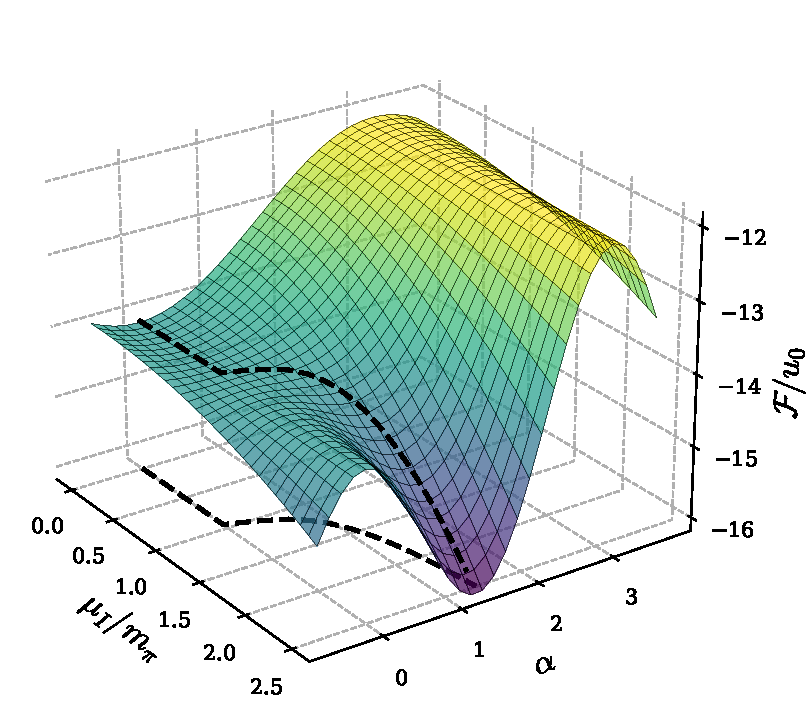
\includegraphics{../scripts/numerikk/plots//free_energy_surface.pdf}
    \caption{
        The free energy surface as a function of $\mu_I$ and $\alpha$. $\alpha$ is the found by minimizing $\Eff$ for a given $\mu_I$. This leads to a curve across the free energy surface, as show in the plot.
        }
    \label{fig: free energy surface}
\end{figure}



\subsection{One-loop contribution}

The one-loop contribution to the free energy density is
%
\begin{equation}
    \label{one loop free energy}
    \Eff^{(1)}
    = - \frac{i}{V T} \frac{1}{2}
    \Tr{\ln\left( -\fdv{S[\pi = 0]}{\pi_a(x), \pi_b(y)} \right)}.
\end{equation}
%
This can be evaluated using the rules for functional differentiation given in \autoref{appendix: Functional derivatives}.
To leading order,
%
\begin{align}
    \fdv{S[\pi = 0]}{\pi_a(x), \pi_b(y)}
    = \fdv{}{\pi_a(x), \pi_b(y)}
    \int \dd^4 x \, \Ell^{(2)}_2
    = D_{ab}^{-1}(x - y).
\end{align}
%
Here, $\Ell^{(2)}_2$ is the quadratic part of the Lagrangian, as given in \autoref{quadratic lagrangian}, and $D^{-1}$ is the corresponding inverse propagator of the pion fields,
\begin{equation}
    D_{ab}^{-1}(x-y) = 
    \left[
        - \delta_{ab}(\partial_x^2 + m^2_a)
        + m_{12}(\delta_{a1} \delta_{b2} - \delta_{a2}\delta_{b1}) \partial_{x, 0}
    \right] \delta(x-y)
\end{equation}
%
The inverse propagator is a matrix, which means that the determinant in \autoref{one loop free energy} is both a matrix determinant, over the three pion indices, and a functional determinant.
In \autoref{section: propagator} we found the matrix part of the determinant in momentum space, which we can write using the dispersion relations of the pion fields
\begin{equation}
    \det(- D^{-1}) = \det(-p_0^2 + E_0^2) \det(-p_0^2 + E_+^2) \det(-p_0^2 + E_-^2).
\end{equation}
%
These dispersion relations are functions of the three-momentum $\vec p$, and are given in \autoref{dispresion relation pi 0} and \autoref{dispresion relation pi pm}.
The functional determinant can therefore be evaluated as
%
\begin{align}
    \nonumber
    \Tr{\ln\left( -\fdv{S[\pi = 0]}{\pi_a(x), \pi_b(y)} \right)}
    & = \ln \det(-p_0^2 + E_0^2) + \ln \det(-p_0^2 + E_+^2) + \ln \det(-p_0^2 + E_-^2) \\
    \nonumber
    & = \Tr{ \ln(-p_0^2 + E_0^2) + \ln(-p_0^2 + E_+^2)+  \ln(-p_0^2 + E_-^2) } \\
    & = (VT) \int \frac{\dd^4 p}{(2 \pi)^4} 
    \left[ \ln(-p_0^2 + E_0^2) + \ln(-p_0^2 + E_+^2) + \ln(-p_0^2 + E_-^2)  \right],
\end{align}
%
where we have used the identity $\ln\det M = \Tr \ln M $.
These terms all have the form
%
\begin{equation}
    \label{free energy logarithmic integral}
    I = \int \frac{\dd^4 p}{(2 \pi)^2} \ln(-p_0^2 + E^2),
\end{equation}
%
where $E$ is some function of the 3-momentum $\vec p$, but not $p_0$.
We use the trick
%
\begin{equation}
    \pdv{}{\alpha} \left(-p_0^2 + E^2\right)^{-\alpha} \Big|_{\alpha=0}
    = \pdv{}{\alpha} \exp\left[ -\alpha \ln\left(- p_0^2 + E^2\right)  \right] \Big|_{\alpha=0}
    = \ln\left(- p_0^2 + E^2\right),
\end{equation}
%
and then perform a Wick-rotation of the $p_0$-integral to write the integral on the form 
%
\begin{equation}
    I = i \pdv{}{\alpha} \int \frac{\dd^4 p}{(2 \pi)^4} \left(p_0^2 + E^2\right)^{-\alpha} \Big|_{\alpha=0},
\end{equation}
%
where $p$ now is a Euclidean four-vector.
The $p_0$ integral equals $\Phi_1(E, 1, \alpha)$, as defined in \autoref{def dimreg integral}. 
The result is therefore given by \autoref{result dimreg},
%
\begin{equation}
    \int \frac{\dd p_0}{2 \pi} (p_0^2 + E)^{-\alpha} 
    = \frac{E^{1-2\alpha}}{\sqrt{4 \pi}} \frac{\Gamma(\alpha-\frac{1}{2})}{\Gamma(\alpha)}.
\end{equation}
%
The derivative of the Gamma function is $\Gamma'(\alpha) = \psi(\alpha)\Gamma(\alpha)$, where $\psi(\alpha)$ is the digamma function.
Using
%
\begin{align}
    \pdv{}{\alpha} & \frac{\Gamma(\alpha - \frac{1}{2}) }{\Gamma(\alpha)} \Big|_{\alpha=0}
    = \Gamma\left(\alpha - \frac{1}{2}\right) \frac{\psi(\alpha - \frac{1}{2}) - \psi(\alpha)}{\Gamma(\alpha)} \Big|_{\alpha=0}
    = \sqrt{4 \pi}, \\
    & \frac{\Gamma(\alpha - \frac{1}{2}) }{\Gamma(\alpha)}\Big|_{\alpha=0} = 0,
\end{align}
%
we get
%
\begin{equation}
    I = i \int \frac{\dd^3 p}{(2 \pi)^3} E.
\end{equation}
%
We see that the result is what we would expect physically; the total energy is the integral of each mode's energy.
This also agrees with the result from \autoref{appendix: thermal field theory} in the zero-temperature limit $\beta \rightarrow \infty$.
The one-loop contribution can therefore be written
%
\begin{equation}
    \Eff^{(1)} = 
    \frac{1}{2} 
    \left[\int \frac{\dd^3 p}{(2\pi)^3} E_0 + \int  \frac{\dd^3 p}{(2\pi)^3} (E_+ + E_-)\right]
    = \Eff^{(1)}_{\pi_0} +\Eff^{(1)}_{\pi_\pm}.
\end{equation}
%
The first integral is identical to what we find for a free field in \autoref{section:free scalar field}, in the zero-temperature limit.
These terms are all divergent and must be regularized.
We will use dimensional regularization, in which the integral is generalized to $d$ dimensions, and the $\overline{\mathrm{MS}}$-scheme, as described in \autoref{section: regualting free energy}.
Using the result for a free field \autoref{free field regularized energy}, we get
%
\begin{equation}
    \label{Free energy pi 0}
    \Eff^{(1)}_{\pi_0} 
    = 
    - \mu^{-2 \epsilon}  \frac{1}{4} \frac{m_3^4}{(4\pi)^2} 
    \left( \frac{1}{\epsilon} + \frac{3}{2} + \ln \frac{\tilde \mu^2}{m_3^2} \right)
    + \mathcal{O}(\epsilon),
\end{equation}
%
where $\mu$ is the renormalization scale, a parameter with mass-dimension 1, introduced to ensure the action integral remains dimensionless during dimensional regularization.
$\tilde \mu$ is a related to $\mu$ as described in \autoref{definition mu tilde MS bar}.

The contribution to the free energy from the $\pi_+$ and $\pi_-$ particles is more complicated, as the dispersion relation is given by
%
\begin{equation}
    E_\pm
    = 
    \sqrt{
        |\vv p|^2 +
        \frac{1}{2}
        \left(
            m_1^2 + m_2^2 + m_{12}^2 
        \right)
        \pm 
        \frac{1}{2}
        \sqrt{
            4|\vv p|^2m_{12}^2 
            +
            \left(
                m_1^2 + m_2^2 + m_{12}^2
            \right)^2
            - 4 m_1^2 m_2^2
        }
    }.
\end{equation}
%
This is not an integral we can easily do in dimensional regularization.
Instead, we will seek a function $f(|\vv p|)$ with the same UV-behavior, that is, behavior for large $\vv p$, as $E_+ + E_-$.
If we then add $0 = f(|\vv p|) - f(|\vv p|)$ to the integrand, we can isolate the divergent behavior
%
\begin{equation}
    \Eff_{\pi_\pm}^{(1)}
    = 
    \frac{1}{2} \int \frac{\dd^3 p}{(2\pi)^3} [E_+ + E_- + f(|\vv p|) - f(|\vv p|)]
    = \Eff^{(1)}_{\mathrm{fin}, \pi_\pm } + \Eff^{(1)}_{\mathrm{div}, \pi_\pm}.
\end{equation}
%
This results in a finite integral,
%
\begin{equation}
    \Eff^{(1)}_{\mathrm{fin}, \pi_\pm } = \frac{1}{2} \int \frac{\dd^3 p}{(2\pi)^3} [E_+ + E_- - f(|\vv p|)],
\end{equation}
%
which we can evaluate numerically, and a divergent integral
%
\begin{equation}
    \Eff^{(1)}_{\mathrm{div}, \pi_\pm }
    = 
    \frac{1}{2} \int \frac{\dd^3 p}{(2\pi)^3} f(|\vv p|),
\end{equation}
%
which we hopefully will be able to do in dimensional regularization.
We can explore the UV-behavior of $E_+ + E_-$ by expanding it in powers of $1 / \abs{\vv{p}}$,
%
\begin{align}
    \nonumber
    E_+ + E_-
    & = 
    2  \abs{\vv{p}}
    + \frac{m_{12} + 2(m_1^2 + m_2^2)}{4} \, {\abs{\vv{p}}}^{-1}
    - \frac{m_{12}^4 + 4 m_{12}^2(m_1^2 + m_2^2) + 8(m_1^4 + m_2^4)}{64}
    {\abs{\vv{p}}}^{-3}
    + \Oh (\abs{\vv{p}}^{-5})
    \\
    & = 
    a_1  \abs{\vv{p}}
    + a_2 \, {\abs{\vv{p}}}^{-1}
    + a_3
    {\abs{\vv{p}}}^{-3}
    + \Oh (\abs{\vv{p}}^{-5}).
\end{align}
%
We have defined new constants $a_i$ for brevity of notation.
As
%
\begin{equation}
    \int_{\R^3} \frac{\dd^3 p}{(2 \pi)^3} |\vv p|^{n}
    = C \int_{0}^\infty \dd p \, p^{2 + n}
\end{equation}
%
is UV divergent for $n \geq -3$, $f$ need to match the expansion of $E_+ + E_-$ up to and including $\Oh(|\vv{p}|^{-3})$ for $\Eff^{(1)}_{\mathrm{fin}, \pi_\pm }$ to be finite.
The most obvious choice for $f$ is
%
\begin{equation}
    f(|\vv p|) 
    = a_1  \abs{\vv{p}} + a_2 \, {\abs{\vv{p}}}^{-1} + a_3 \, {\abs{\vv{p}}}^{-3}.
\end{equation}
%
However, this introduces a new problem.
$f$ has the same UV-behavior as $E_+ + E_-$, but the last term diverges in the IR, that is, for low $|\vv p|$.
This can be amended by introducing a mass term.
Let
%
\begin{equation}
    |\vv p|^{-3} 
    = 
    \left(\frac{1}{\sqrt{|\vv p|^2}}\right)^3 
    \longrightarrow 
    \left(\frac{1}{\sqrt{|\vv p|^2 + m^2}}\right)^3.
\end{equation}
%
For $|\vv p|^2 \rightarrow \infty$, this is asymptotic to $|\vv p|^{-3}$, so it retains its UV behavior.
However, for $|\vv p| \rightarrow 0$, it now approaches $m^{-3}$, so the IR-divergence is gone.
The cost of this technique is that we have introduced an arbitrary mass parameter.
Any final result must thus be independent of the value of $m$ to be acceptable.

We will instead regularize the integral by defining $E_i = \sqrt{|\vv{p}|^2 + \tilde m_i^2}$, and $\tilde m_i^2 = m_i^2 + \frac{1}{4} m_{12}^2$.
Using the definition of the masses, \autoref{m1}, \autoref{m2}, \autoref{m3}, and \autoref{m12}, we get
%
\begin{align}
    m_3^2 & = \bar m^2 \cos \alpha + \mu_ I^2 \sin^2 \alpha, \\
    \label{tilde m1}
    \tilde m_1^2 
    & 
    = m_1^2 + \mu^2 \cos\alpha^2
    = \bar m^2 \cos \alpha + \mu_I^2 \sin^2 \alpha
    = m_3^2 \\
    \label{tilde m2}
    \tilde m_2^2 
    & = m_2^2 + \mu^2 \cos\alpha^2
    = \bar m^2 \cos \alpha.
\end{align}
%
Finally, we define $f(|\vv p|) = E_1 + E_2$, which differ from $E_+ + E_-$ by $\Oh\left(|\vv p|^{-5}\right)$ and is well-behaved in the IR.
This leads to a divergent integral the same form as in the case of a free scalar.
Thus, in the $\mathrm{\overline{MS}}$-scheme, 
%
\begin{equation}
    \Eff^{(1)}_{\mathrm{div}, \pi_\pm }
    =
    - \mu^{-2 \epsilon} \frac{1}{4} \frac{\tilde m_1^4}{(4\pi)^2} 
    \left(
        \frac{1}{\epsilon} + \frac{3}{2} + \ln \frac{\tilde \mu^2}{\tilde m_1^2}
    \right) 
    -  \mu^{-2 \epsilon} \frac{1}{4} \frac{\tilde m_2^4}{(4\pi)^2} 
    \left(
        \frac{1}{\epsilon} + \frac{3}{2} + \ln \frac{\tilde \mu^2}{\tilde m_2^2}
    \right) 
    + \mathcal{O}(\epsilon).
\end{equation}
%
We define
%
\begin{equation}
    \Eff^{(1)}_{\mathrm{fin}, \pi_\pm}
    = 
    \frac{1}{2} \int \frac{\dd^3 p}{(2\pi)^3} (E_+ + E_- - E_1 - E_2),
\end{equation}
%
which is a finite integral.
The total one-loop contribution is then, using \autoref{tilde m1} and \autoref{tilde m2},
%
\begin{align}
    \Eff^{(2)}
    & = 
    \Eff^{(1)}_{\mathrm{fin}, \pi_\pm}
    - \mu^{-2 \epsilon} \frac{1}{2}\frac{1}{(4\pi)^2}
    \left[
        \left( \frac{1}{\epsilon} + \frac{3}{2} + \ln \frac{\tilde \mu^2}{m_3^2 } \right)
        m_3^4
        +
        \frac{1}{2}
        \left( \frac{1}{\epsilon} + \frac{3}{2} + \ln \frac{\tilde \mu^2}{\tilde m_2^2} \right)
        \tilde m_2^4
    \right]
    + \Oh(\epsilon).
\end{align}


    \section{*Next-to-leading order and renormalization}

We have now regularized the divergences, which allows them to be handled in a well-defined way.
However, they are still there.
To get rid of them, we need to use renormalization.
As laid out in \autoref{section: chiral perturbation theory}, the power counting scheme ensures that all terms in $\Ell_{2n}$ scales as $t^{2n}$ when the momenta $p$ are scaled as  $p \rightarrow t p$.\footnote{
    Remember that we scale pion mass $\bar m = B_0(m_u + m_d)$ as $t^2$, and the chemical potential as $t$.
    }
The tree-level free energy from $\Ell_{2n}$ is thus of order $p^{2n}$.
The $m$-loop correction to the tree level result is then suppressed by $p^{2m}$~\autocite{gasserChiralPerturbationTheory1984,weinbergPhenomenologicalLagrangians1979}.
Our one-loop calculation using $\Ell_2$ therefore contains divergences of order $p^{4}$. 
Since $\Ell_4$ is, by construction, the most general possible Lagrangian at order $p^4$, it contains coupling constants that can be renormalized to absorb all these divergences.

The renormalized coupling constants in $\Ell_4$ have been calculated for $\mu_I = 0$\autocite{gasserChiralPerturbationTheory1984}.
They are independent of $\mu_I$, and we can therefore use them in this calculation.
The renormalized coupling constants in the $\overline{\mathrm{MS}}$-scheme are related to the bare couplings through
%
\begin{align}
    l_i 
    & = 
    l_i^r 
    - \mu^{-2\epsilon}\frac{1}{2} \frac{\gamma_i }{(4 \pi)^2} 
    \left(\frac{1}{\epsilon} + 1 \right),
    \quad \quad
    i \in \{1, ... 7\},
    \\
    h_i 
    & = 
    h_i^r
    - \mu^{-2\epsilon} \frac{1}{2}  \frac{\delta_i }{(4 \pi)^2} 
    \left(\frac{1}{\epsilon} + 1 \right), 
    \quad \quad
    i \in \{1, ... 3\}.
\end{align}
%
Here, $\gamma_i$ and $\delta_i$ are numerical constants which are used to match the divergences.
The relevant terms are\footnote{Some authors~\autocite{adhikariTwoflavorChiralPerturbation2019,gerberHadronsChiralPhase1989} instead use $h_1' = h_1 - l_4$, with a corresponding $\delta_1' = \delta_1 - \gamma_1 = 0$.}
%
\begin{gather}
    \gamma_1 = \frac{1}{3}, \quad
    \gamma_2 = \frac{2}{3}, \quad
    \gamma_3 = - \frac{1}{2}, \quad
    \gamma_4 = 2, \\
    \delta_1 = 2, \quad
    \delta_3 = 0.
\end{gather}
%
The bare coupling constants $l_i$ and $h_i$, though infinite, are independent of our renormalization scale $\mu$.
From this we obtain the renormalization group equations for the running coupling constants,
\begin{equation}
    \mu \odv{l_i^r}{\mu } = - \mu^{-2\epsilon} \frac{\gamma_i }{(4 \pi)^2} + \mathcal{O}(\epsilon), \quad
    \mu \odv{h_i^r}{\mu } = -  \mu^{-2\epsilon}\frac{\delta_i}{(4 \pi)^2}+ \mathcal{O}(\epsilon).
\end{equation}
%
These have the general solutions
\begin{equation}
    l_i^r 
    = \frac{1}{2} \mu^{-2\epsilon} \frac{\gamma_i}{(4 \pi)^2} 
    \left( \bar l_i - \ln{\frac{\tilde \mu^2}{M^2}} \right)+ \mathcal{O}(\epsilon),
    \quad
    h_i^r 
    = \frac{1}{2} \mu^{-2\epsilon} \frac{\gamma_i}{(4 \pi)^2} 
    \left( \bar h_i - \ln{\frac{\tilde \mu^2}{M^2}} \right)+ \mathcal{O}(\epsilon),
\end{equation}
%
where $\bar l_i$ and $\bar h_i$ are the values of the coupling constants (times a constant) measured at the energy $M$.
This only applies if the numerical constants $\gamma_i$/$\delta_i$ are non-zero.
If they are zero, then the coupling is not running, and the measured value can be applied at all energies.
The bare couplings are thus given by
\begin{align}
    \label{bare couplings as functions of measured values}
    l_i &= \mu^{-2\epsilon} \frac{1}{2} \frac{\gamma_i}{(4 \pi)^2}
    \left(
        \bar l_i -1- \frac{1}{\epsilon} - \ln\frac{\tilde \mu^2}{M^2}
    \right)+ \mathcal{O}(\epsilon), \\
    h_i &= \mu^{-2\epsilon} \frac{1}{2} \frac{\delta_i}{(4 \pi)^2}
    \left(
        \bar h_i - 1 - \frac{1}{\epsilon} - \ln\frac{\tilde \mu^2}{M^2}
    \right)
    + \mathcal{O}(\epsilon).
\end{align}
%
The next-to-leading contribution to the free energy at tree-level is $\Eff_4^{0} = - \Ell_4^{(0)}$, which is given by \autoref{NLO-L0}.
When substituting \autoref{bare couplings as functions of measured values} into the bare couplings, we get
%
\begin{align*}
    \Eff^{(0)}_4
    & = 
    - (l_1 + l_2)\mu_I^4 \sin^4{\alpha}
    - (l_3 + l_4)\bar m^4 \cos^2{\alpha}
    - l_4 \bar m^2 \mu_I{}^2 \cos{\alpha} \sin^2{\alpha}
    -(h_1- l_4) \bar m^4
    - h_3 \Delta m^4
    \\
    & = 
    - \mu^{-2 \epsilon} \frac{1}{2} \frac{1}{(4 \pi)^2}
    \bigg[
        \frac{1}{3}
        \left( 
            \bar l_1 + 2 \bar l_2 - 3
        \right) \mu_I^4 \sin^4 \alpha
        +
        \frac{1}{2}
        \left(
            - \bar l_3 + 4 \bar l_4 - 3
        \right) \bar m^4 \cos^2\alpha
        \\
        & \quad \quad \quad \quad \quad \quad \quad
        + 2 \left(\bar l_4 - 1\right)
        \bar m^2 \mu_I^2 \cos\alpha \sin^2 \alpha
        + 2 (\bar l_4 - \bar h_1) \bar m^4
        + \bar h_3 \Delta m^4
        \\
        & \quad \quad \quad \quad \quad \quad \quad
        - 
        \left(\frac{1}{\epsilon} + \ln \frac{\tilde \mu^2}{M^2}\right) 
        \left(
            \mu_I^4\sin^4\alpha + \frac{3}{2} \bar m^4 \cos^2 \alpha
            + 2 \bar m^2 \mu_I^2 \cos\alpha \sin^2 \alpha
        \right) 
    \bigg] + \mathcal{O}(\epsilon).
\end{align*}
%
Notice that the term proportional to $\epsilon^{-1}$ cancel exactly with the divergent term from $\Eff^{(2)}$, as we expected.
Adding all the contribution to the free energy density, and taking the limit $\epsilon \rightarrow 0$, we get the next-to-leading order free energy density,
%
\begin{align}
    \nonumber
    \Eff_{\mathrm{NLO}} &=
    - f^2 \left(\bar m^2 \cos \alpha + \frac{1}{2}\mu_I^2 \sin^2 \alpha\right)
    + \Eff^{(1)}_{\mathrm{fin}, \pi_\pm}
    - \frac{1}{2}\frac{1}{(4 \pi)^2}
    \bigg[
        \frac{1}{3}
        \left( 
            \bar l_1 + 2 \bar l_2 + \frac{3}{2} + 3 \ln \frac{M^2}{m_3^2}
        \right) \mu_I^4 \sin^4 \alpha
        \\ %\nonumber
        &
        +
        \frac{1}{2}
        \left(
            - \bar l_3 + 4 \bar l_4 + \frac{3}{2} + 2\ln \frac{M^2}{m_3^2}
            + \ln \frac{M^2}{\tilde m^2_2}
        \right) \bar m^4 \cos^2\alpha 
        + 2 \left(\bar l_4 + \frac{1}{2} + \ln \frac{M^2}{m_3^2}\right)
        \bar m^2 \mu_I^2 \cos\alpha \sin^2 \alpha
        \label{NLO free energy}
    \bigg].
\end{align}
%
We have dropped the terms proportional to $\bar l_4 - \bar h_1$ and $\bar h_3$, as they only add an unobservable constant value to the free energy.


\subsection{Parameters and consistent expansion}

The coupling constants are free parameters of the effective theory of \chpt.
As we are not able to do calculations with QCD at low energies, these must be measured instead of calculated from first principles.
The values for the pion mass and pion decay constants used in this text are
\todo[]{use correct values}
%
\begin{equation}
    m_\pi = 131 \, \mathrm{MeV}, \quad 
    f_\pi = \frac{1}{\sqrt 2} 128 \, \mathrm{MeV} = 90.5 \, \mathrm{MeV}.
\end{equation}
%
The most up-to-date value of the pion masses from the Pardicle Data Book are~\cite{particledatagroupReviewParticlePhysics2020}
\todo[]{sammkjør verdier}
%
\begin{equation}
    m_0 = 139.57039\pm0.00018\, \text{MeV}, \quad
    m_\pm = 134.9768\pm0.0005\, \text{MeV}.
\end{equation}
%
These are the masses of the neutral and the charged pions and includes contribution due to electromagnetic and weak interactions, which are not included in this study.
The value for the pion decay constant is~\cite{particledatagroupReviewParticlePhysics2020}
%
\begin{equation}
    f_\pi = \frac{1}{\sqrt{2}} (130.2 \pm 1.2 \, \text{MeV})
    = 92.1 \pm 0.8 \, \text{MeV}.
\end{equation}
%

The physical mass, $m_\pi$, is defined as the pole of the propagator in the vacuum, and thus the zero of the inverse propagator,
%
\begin{equation}
    D^{-1}(p^2 = m_\pi^2) = 0.
\end{equation}
%
This relates it to the bare mass $\bar m$.
We found, in \autoref{m1}, that $m_\pi^2 = \bar m^2$ to leading order.
Similarly, $f_\pi = f$ to leading order.
However, in any NLO results we need the relationship between the bare and physical constants to NLO.
This is given by~\autocite{gasserChiralPerturbationTheory1984}
%
\begin{align}
    \label{equation bare mass}
    m_\pi^2 & = \bar m^2 + \frac{\bar l_3}{2 (4\pi)^2} \frac{\bar m^4}{f^2}, \\
    \label{equation bare decay constant}
    f_\pi^2 & = f^2 + \frac{2\bar l_4}{(4\pi)^2} \frac{\bar m^2}{f^2}.
\end{align}
%

\begin{table}[h]
    \centering
    \caption{The measured values and corresponding uncertainties of the relevant coupling constants, measured at $M = m_\pi$.}
    \begin{tabular}{c c c c}
        \hline \hline
        & value & uncertainty & source \\
        \hline \\[-1em]
        $\bar l_1$ & -0.4 & \pm 0.6   & \autocite{colangeloPpScattering2001}    \\
        $\bar l_2$ & 4.3  & \pm 0.1   & \autocite{colangeloPpScattering2001}   \\
        $\bar l_3$ & 2.9  & \pm 2.4   & \autocite{gasserChiralPerturbationTheory1984}\\
        $\bar l_4$ & 4.4  & \pm 0.2   & \autocite{colangeloPpScattering2001}    \\
        \hline
    \end{tabular}
    \label{table: coupling constants}
\end{table}
%
The values for the coupling constants used in this text are given in \autoref{table: coupling constants}.
The constants $\bar l_1$, $\bar l_2$ and $\bar l_4$ are estimated using data from $\pi \pi$-scattering~\autocite{colangeloPpScattering2001}, while $\bar l_3$ is estimated using three flavor chiral perturbation theory~\autocite{gasserChiralPerturbationTheory1984}.
These are the same values as those used in~\autocite{adhikariTwoflavorChiralPerturbation2019}.
In this text, we use the central values of the parameters.
Together with \autoref{equation bare mass}\autoref{equation bare decay constant}, the NLO results for the central value for the bare mass and decay constant are
%
\begin{align}
    \label{NLO m}
    \bar m  &= 1.01136\, m_\pi = 132.5 \, \mathrm{MeV}, \\
    \label{NLO f}
    f  &= 0.64835\, m_\pi = 85.9 \, \mathrm{MeV}.
\end{align}
%

In \autoref{section: free energy at lowest order}, we found a relationship between $\alpha$ and $\mu_I$, using the lowest-order result for $\Eff$, given in \autoref{leading order minimization}.
To calculate any thermodynamic quantities to leading order, at tree-level, we must use this result.
When using the NLO result for the free energy, we must consistently calculate this and other quantities to the same order.
As we have seen earlier, when replacing the action by $S[\varphi] \rightarrow g^{-1}S[\varphi]$, the $L$-loop contribution is proportional to $g^{L-1}$.
In Weinberg's power counting scheme, as laid out in \autoref{section: chiral perturbation theory}, we scale $p \rightarrow t p$ and $m_q \rightarrow t^2 m_q$.
Then, the $n$th term in the expansion is proportional to $t^{2n}$.
We can therefore expand the free energy as
\begin{equation}
    \Eff = t^2 g^{-1} \Eff_2^{(0)} + t^2 \Eff_2^{(1)} + t^4 g^{-1} \Eff_4^{(0)}
    + ...
\end{equation}
%
We consider terms where $k = L + n$ has the same value to be of same order.
This expansion can be written as
\begin{equation}
    \Eff = \sum_{k=0}^\infty \sum_{n+L=k} t^{2n} g^{L-1} \Eff_{2n}^{(L)}.
\end{equation}
%
If we now define
\begin{equation}
    \tilde \Eff_k = \sum_{n+L=k} t^{2n} g^{L-1} \Eff_{2n}^{(L)},
\end{equation}
%
then scale $t \rightarrow \sqrt{s} \, t$ and $g \rightarrow s g$, where $s$ is some real number, then $t^{2n}g^{L-1}$ scales as $s^{n+L-1} = s^{m-1}$.
All expansions are now done in this new parameter $s$.
The free energy expansion is
\begin{equation}
    \Eff = s^{-1}\sum_{k = 0}^\infty \tilde \Eff_k \, s^{k}.
\end{equation}
%
As argued earlier, $\alpha$ must minimize the free energy, and therefore satisfy
%
\begin{equation}
    \pdv{\Eff}{\alpha} = 0,
\end{equation}
%
to all orders.
We expand this solution in $s$,
\begin{equation}
    \alpha = \alpha_0 + \alpha_1 s + \dots.
\end{equation}
%
Combining this, we get
%
\begin{align}
    \nonumber
    0 &
    = 
    \pdv{}{\alpha}
    \left[
        s^{-1}\tilde \Eff_0
        + 
        \tilde \Eff_1
        +
        \Oh(s)
    \right]
    \bigg|_{\alpha=\alpha_0 + \alpha_1 s + \Oh{s}} 
    \\ \nonumber
    & = 
    s^{-1 }
    \left[
        \tilde \Eff_0'(\alpha_0)
        +
        (\alpha' - \alpha_0)
        \tilde \Eff_0''(\alpha_0)
        +
        \Oh(s^2)
    \right]
    +
    \tilde\Eff_1'(\alpha_0)
    +
    \Oh(s) \\
    &
    =
    s^{-1} \tilde\Eff_1'(\alpha_0)
    + s^{0}
    \left[
        \alpha_1
        \tilde \Eff_0''(\alpha_0)
        +
    \tilde\Eff_1'(\alpha_0)
    \right]
    +
    \Oh(s).
    \label{minimizing free energy expansion}
\end{align}
%
Here, the prime indicates partial derivatives with respect to $\alpha$.
The equality in \autoref{minimizing free energy expansion} has to hold term for term.
After setting $s = g = t = 1$, we get
%
\begin{align*}
    \pdv{\tilde \Eff_0}{\alpha}\bigg|_{\alpha=\alpha_0} = 0, \quad
    \tilde \Eff_0 = \Eff_2^{(0)},
\end{align*}
%
which is what we have used as the leading-order result. 
The first correction is on this result is
%
\begin{equation}
    \label{NLO correction alpha}
    \alpha_1 = - \frac{\tilde \Eff_1'(\alpha_0)}{{\tilde \Eff_0''(\alpha_0)}},
    \quad 
    \tilde \Eff_1 = \Eff_{4}^{(0)} + \Eff_{2}^{(1)}.
\end{equation}
%

The next to leading order results for the free energy and $\alpha$ are
%
\begin{equation}
    \Eff_\mathrm{NLO} = \tilde \Eff_0 + \tilde \Eff_1, \quad
    \alpha_\mathrm{NLO} = \alpha_0 + \alpha_1.
\end{equation}
%
We have that
%
\begin{equation}
    \Eff_\mathrm{NLO}'(\alpha_\mathrm{NLO})
    = \tilde \Eff_0'(\alpha_0) + \alpha_1 \tilde \Eff_0''(\alpha_0) + \dots
    + \tilde \Eff_1'(\alpha_0) + \dots,
\end{equation}
%
where the excluded terms are beyond next-to-leading order.
Using \autoref{NLO correction alpha}, we see that this vanishes to next-to-leading order.
We therefore use the criterion
%
\begin{equation}
    \label{alpha nlo method 2}
    \pdv{\Eff_\mathrm{NLO}}{\alpha} \bigg|_{\alpha=\alpha_{\mathrm{NLO}}} = 0
\end{equation}
%
to calculate $\alpha_\text{NLO}$.
The result is shown in \autoref{fig: alpha}, which compares the leading order and next-to-leading order results for $\alpha$.

\todo[]{fiks figur}
\begin{figure}
    \centering
    % \includegraphics[width=0.7\textwidth]{../scripts/numerikk/plots/alpha.pdf}
    \caption{The leading order and next-to-leading order results for $\alpha$ as a function of $\mu_I$, which is given in units of $m_\pi$. }
    \label{fig: alpha}
\end{figure}

We can use the expansion in $s$ to consistently evaluate any observable to any power in perturbation theory.
Assume that $f$ is some obserable, and a function of $\alpha$.
We then expand in $s$,
%
\begin{equation}
    f(\alpha) = f_0(\alpha) + s f_1(\alpha) + s^2 f_2(\alpha) + \dots
\end{equation}
%
When Taylor expanding around the leading order result for $\alpha$, we get
%
\begin{align*}
    f(\alpha) 
    & 
    = 
    f_0(\alpha_0)
    +
    s\alpha_1  f_0'(\alpha_0)
    +
    s f_1(\alpha_0)
    + \Oh(s^2)
    = f_0(\alpha_0 + s \alpha_1)
    + s f_1(\alpha_0)
    + \Oh(s^2).
\end{align*}
%
We see that, to get a consistent expansion, we must evaluate the leading order result for the function $f_0$ at next-to-leading order in $\alpha$, while next-to-leading order correction can be evaluated at leading order.
However, as
%
\begin{equation}
    f_1(\alpha_0 + s\alpha_1) = f_1(\alpha_0) + \Oh(s),
\end{equation}
%
we also get a consistent expansion if we evaluate the leading-order result and its correction at next-to-leading order in $\alpha$.
We will do this to obtain the results in the next section.

    \section{*Equation of state}
\label{section: equation of state}


The methods and analysis of this section are based on~\autocite{adhikariTwoflavorChiralPerturbation2019,andersenIntroductionStatisticalMechanics2012,peskinIntroductionQuantumField1995}.
All results in this section are given in units of $m_\pi$.

The free energy\footnote{
    As we are in the grand canonical ensemble, this is the grand canonical, or Landau, free energy, also called the grand potential, and not Helmholtz' free energy.
    }
is defined as
%
\begin{equation}
    \label{thermodynamic free energy}
    F(T, V, \mu_I) = U - TS - \mu_I Q_I, 
    \quad \dd 
    F = - S \dd T - P \dd V - Q_I \dd \mu_I.
\end{equation}
%
In our case, all results are for $T = 0$.
As we have seen earlier, our system is homogenous.
This means that the free energy density is independent of volume, and thus $F = V \Eff$.
From \autoref{thermodynamic free energy}, the pressure is given by
%
\begin{equation}
    P = - \left(\pdv{F}{V}\right)_{T, \mu_I} = - \Eff.
\end{equation}
%
We are interested in the pressure relative to the state in which $\mu_I$ = 0. We therefore normalize $P(\mu_I=0) = 0$, which gives  
%
\begin{equation}
    P(\mu_I) = -[\Eff(\mu_I) - \Eff(\mu_I = 0)].
\end{equation}
%
\todo[]{fiks fig}
This is illustrated in \autoref{fig: pressure}.

\begin{figure}[h]
    \centering
    \vspace{-0.2cm}
    % 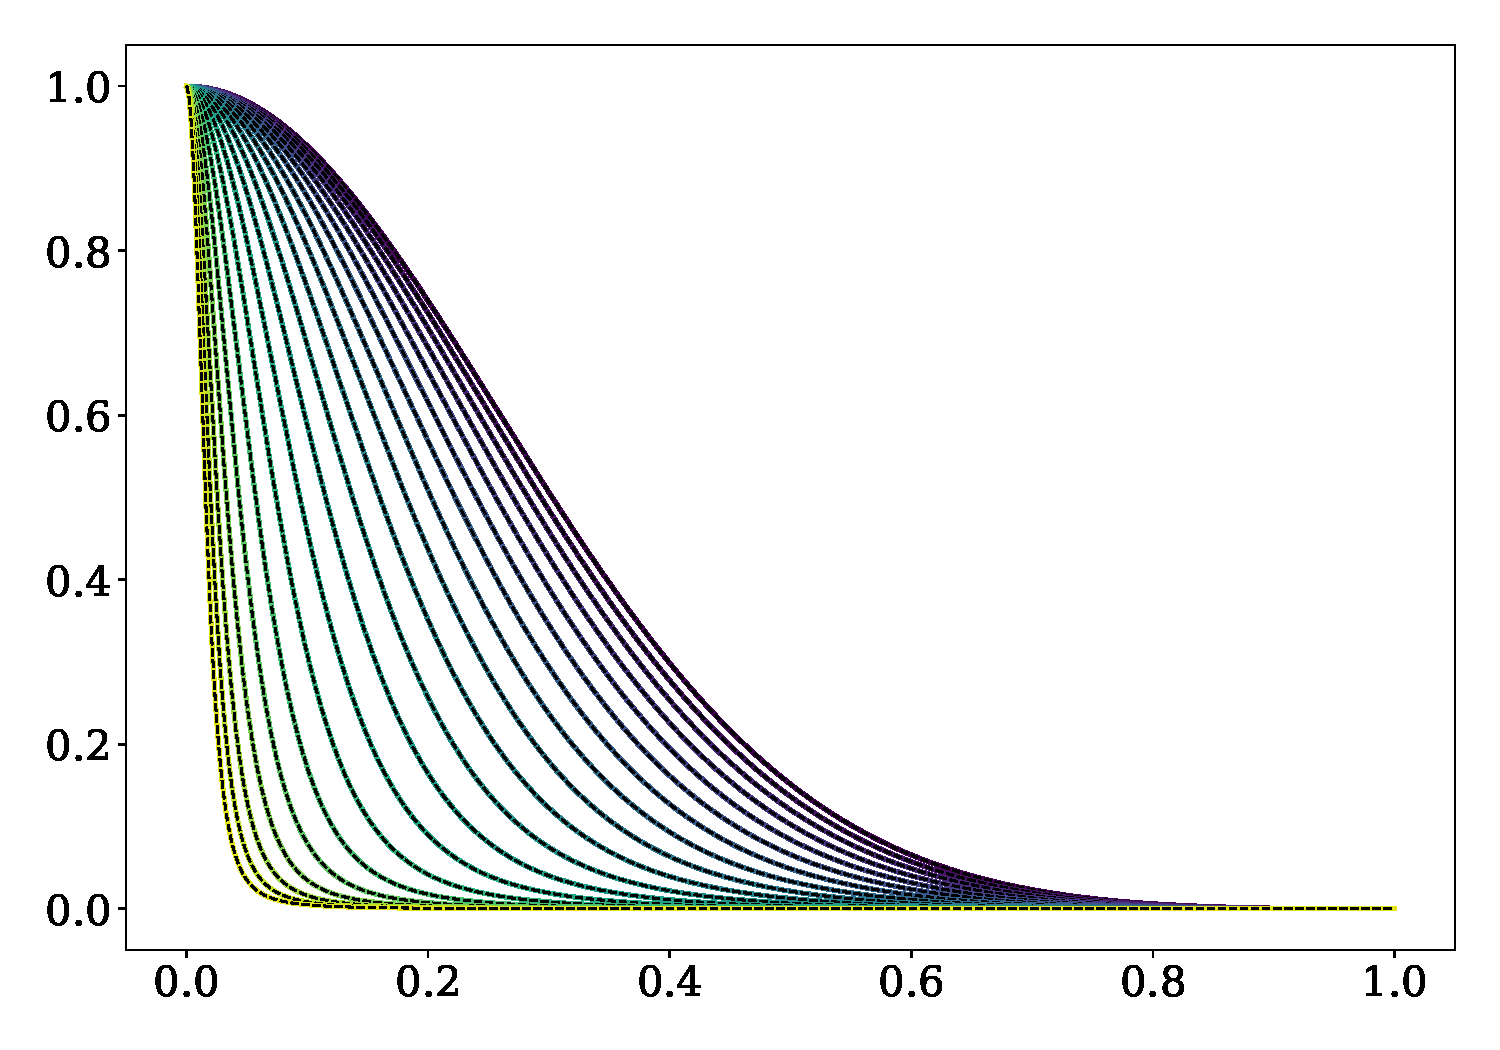
\includegraphics[width=0.7\textwidth]{../scripts/numerikk/plots/pressure.pdf}
    \caption{The LO and NLO result for the pressure, as a function of $\mu_I$.}
    \label{fig: pressure}
\end{figure}

Likewise, the total isospin is proportional to volume, which means that the isospin density is
%
\begin{equation}
    n_I = \frac{Q_I}{V} = - \frac{1}{V} \left(\pdv{F}{\mu_I}\right)_{T, V}
    = - \pdv{\Eff}{\mu_I}.
\end{equation}
%
Using \autoref{NLO free energy}, this equals
%
\begin{align}
    \nonumber
    n_I & = 
    f^2 \mu_I \sin^2 \alpha
    - \pdv{\Eff_\mathrm{fin}}{\mu_I} \\
    & + \frac{1}{(4 \pi)^2}
    \left[
            \left(
                2\bar l_4+\ln\frac{M^2}{m_3^2}
            \right) 
            \bar m^2 \mu_I \cos\alpha \sin^2 \alpha
            +\frac{1}{3}
            \left(
                2\bar l_1 + 4 \bar l_2 + 3\ln\frac{M^2}{m_3^2}
            \right)
            \mu_I^3 \sin^4 \alpha
    \right].
\end{align}
%
The isospin density, as a function of $\mu_I$, is shown in \autoref{fig: isospin_density}.
\todo[]{fiks fig}
\begin{figure}[h]
    \centering
    \vspace{-0.2cm}
    % \includegraphics[width=0.7\textwidth]{../scripts/numerikk/plots/isospin_density. pdf}
    \caption{The LO and NLO result for the isospin density, as a function of $\mu_I$.}
    \label{fig: isospin_density}
\end{figure}

From \autoref{thermodynamic free energy} we get the energy density, $u = U/V$, at $T = 0$, is given by
%
\begin{equation}
    u(\mu_I) = -P(\mu_I) + \mu_I n_I(\mu_I),
\end{equation}
%
where we again have normalized so that $u(\mu_I = 0) = 0$.
Now that we have both the dependence of the pressure and the energy density on the isospin chemical potential, we can trace out the line in the pressure-energy density plane, parametrized by $\mu_I$.
This is the equation of state of the system and is shown in \autoref{fig:equation of state}.
\todo[]{fiks fig}

\begin{figure}[h]
    \centering
    % \vspace{-0.2cm}
    % \includegraphics[width=0.7\textwidth]{../scripts/numerikk/plots/eos.pdf}
    \caption{Th e leading and next-to-leading order equation of state. Both the pressure and energy density are given in units of $m_\pi^4$.}
    \label{fig:equation of state}
\end{figure}

% delta E = -0.07170144633730757
% delta P = -0.02590428743830242

The next-to-leading order correction is small compared to the leading order result.
The maximum correction to the energy density is $0.0717 \, m_\pi^4$, while the largest correction to the pressure is $0.02590\, m_\pi^4$.
We notice that the difference steadily increases with the value of $\mu_I$.
This is expected, as the perturbation theory assumes small disturbances.

As both the pressure and isospin density are zero for $\mu_I < m_\pi$, the equation of state in the vacuum phase is trivial.
It is only for $\mu_I \geq m_\pi$ that we get interesting behavior.
We see that this is a recurring theme.
The vacuum and the next quantum state are separated by a finite energy gap, given by the mass of the lightest particle.
We see this from the energies we found for $\mu_I < 0$, \autoref{zeeman energy}\autoref{zeeman energy 2}, which gave a Zeeman-like splitting.
As the isospin chemical potential smoothly varies from zero, the free energy becomes different from the vacuum energy.
A system in equilibrium minimizes the free energy. 
However, due to the finite gap between the vacuum and other states, we expect there to be a critical value $\mu_I^c$ below which all observable quantities are independent of $\mu_I$.
This is called the ``Silver-Blaze'' property~\autocite{cohenQCDInequalitiesNucleon2003,gunkelMesonsFiniteChemical2020}.


    \section{*Phase transition}
\label{section: phase transition}


Our leading-order analysis showed that $\alpha$ is zero for $\mu_I \leq \bar m$ and then increases continuously for $\mu_I>\bar m$.
Furthermore, $\bar m = m_\pi$ to leading-order.
This behavior is illustrated in \autoref{fig: alpha}.
This is the hallmark of a phase transition, where $\alpha$ is the order parameter.
The behavior of systems near points of phase transition is described by Landau theory~\autocite{peskinIntroductionQuantumField1995}.
Using \autoref{leading order contribution free energy}, we can expand the leading-order free energy in $\alpha$,
%
%
\begin{align}
    \nonumber
    \Eff
    & = -f^2 \bar m^2 + f^2 \frac{1}{2}(\bar m^2 - \mu_I^2)\alpha^2
    - \frac{1}{24} f^2 (\bar m^2 - 4 \mu_I^2) \alpha^4 + \Oh(\alpha^5)\\
    & = \Eff(\alpha=0) + a(\mu_I)\alpha^2 + \frac{1}{2} b(\mu_I)\alpha^4 + \Oh(\alpha^5).
\end{align}
%
Notice that near $\mu_I = \bar m$, $b > 0$.
As earlier, the equation that governs $\alpha$ is
%
\begin{equation}
    \label{landau ginsburg lo}
    \pdv{\Eff}{\alpha} = 2 [a(\mu_I) + b(\mu_I) \alpha^2] \alpha = 0.
\end{equation}
%
If $a>0$, then $\alpha = 0$ will be the only solution, which gives us the criterion for a phase transition
%
\begin{equation}
    a(\mu_I) = 0.
\end{equation}
%
As expected, this criterion is fulfilled at $\mu_I = \bar m$.
Near $\mu_I = \bar m$, we can write
%
\begin{equation}
    a = - a_0 (\mu_I - \bar m), \quad b = b_0,
\end{equation}
%
where $a_0$ and $b_0$ are positive constants, so the solution to \autoref{landau ginsburg lo} for $\mu_I>\bar m$ is
%
%
\begin{equation}
    \alpha(\mu_I) = \sqrt{\frac{a_0}{b_0}} (\mu_I - \bar m)^{1/2}.
\end{equation}
%
The free energy around the phase transition is illustrated in \autoref{fig: phase transition}.
\todo[]{fiks figur}

\begin{figure}[h]
    \centering
    % 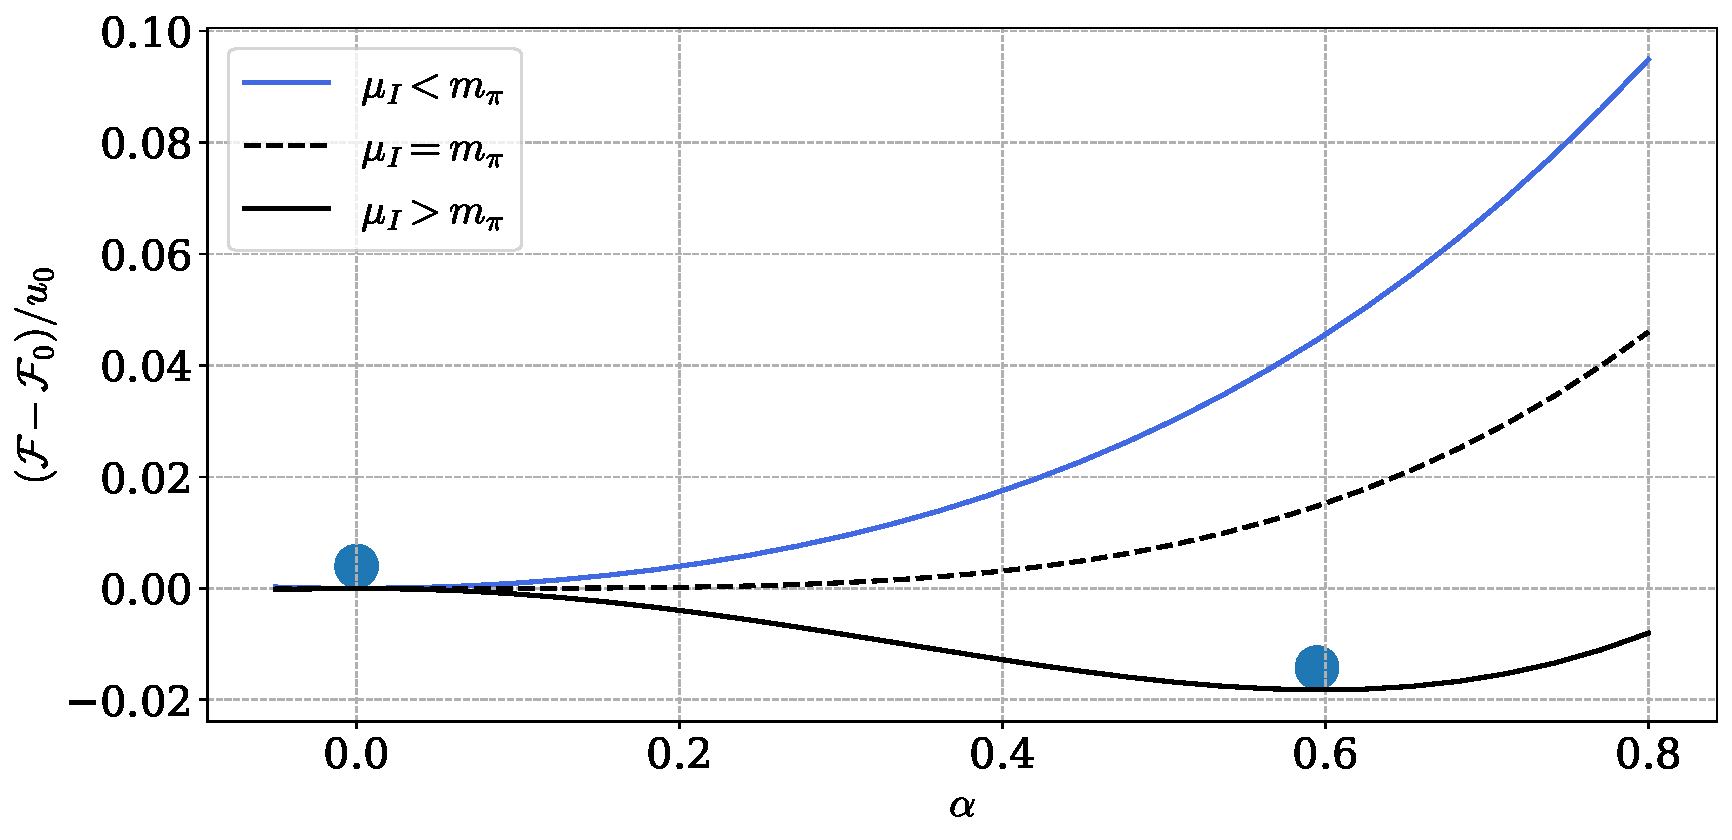
\includegraphics[width=0.9\textwidth]{../scripts/numerikk/plots/phase_transition.pdf}
    \caption{
        The plot shows normalized free energy density as a function of $\alpha$, in the two different phases. Each line is a constant $\mu_I$ slice of the surface in \autoref{fig: free energy surface}.
        }
    \label{fig: phase transition}
\end{figure}

The order parameter $\alpha$ changes continuously as the system transitions between phases.
This means we have a \emph{second order} phase transition.
The power-law behavior, $\alpha \propto (\mu_I - \mu_I^c)^\beta$, is typical of systems near a phase transition.
The exponent $\beta$, which in this case equals $1/2$, is called a \emph{critical exponent}.
If we have a system where $b < 0$ near $\mu_I = \bar m$, then we must expand $\Eff$ further to show if the phase transition is continuous or not.
\autoref{fig: free energy surface 2} shows the free energy surface but modified so that $b_0 < 0$, together with the corresponding value of $\alpha$, which now changes discontinuously at the point of phase transition.
\todo[]{fiks fig}

\begin{figure}[h]
    \centering
    % \includegraphics[width=0.7\textwidth]{../scripts/numerikk/plots/free_energy_surface2.pdf}
    \caption{The surface is free energy density, only modified so that $b_0<0$. The black line traces out the minimum for each value of $\mu_I$, which jumps discontinuously at the point of phase transition.}
    \label{fig:free energy surface 2}
\end{figure}


In the vacuum phase, $\alpha = 0$, the ground state is given by 
%
\begin{equation}
    \Sigma(\pi = 0) = \Sigma_0 = \one,
\end{equation}
%
where we have used \autoref{sigma}.
Under $H = SU(2)_V$, $\Sigma$ transforms as
%
\begin{equation}
    \Sigma(x) \rightarrow \Sigma'(x) = U_V \Sigma(x) U_V^\dagger,
    \quad
    V = \exp{i \frac{1}{2} \theta_a \tau_a},
\end{equation}
%
We see that the vacuum phase ground state is invariant under $H$.
However, for $\alpha \neq 0$, the ground state is shifted to
%
\begin{equation}
    \Sigma(\pi=0) = A_\alpha \Sigma_0 A_\alpha = \exp{i \alpha \tau_1}.
\end{equation}
%
This is not, in general, invariant under transformations in $H$. 
The generators $\tau_2$ and $\tau_3$ are broken.
In \autoref{fig: masses}, we saw that the mass of the $m_-$ particle vanishes, so we identify this particle with the corresponding Goldstone mode.
There is only one Goldstone mode. 
However, this is not a Lorentz invariant system, in which case we cannot guarantee one massless mode per broken generator.
In \autoref{section: leading order}, we defined
%
\begin{equation}
    \alpha = \frac{1}{f} \sqrt{\pi_a^0 \pi_a^0},
\end{equation}
%
where $\pi_a^0$ was the ground state expectation value of the pion fields, as defined in the vacuum phase, when $\mu_I \neq 0$.
The new ground state thus corresponds to a condensate of pions.
The isospin symmetry $\Lie{SU}{2}_V$ is not a perfect symmetry of the QCD Lagrangian, but is explicitly broken by the mass term
\begin{equation}
    \bar q m q = \frac{1}{2} \bar q [(m_u + m_d) \one + (m_u - m_d)\tau_3] q.
\end{equation}
%
This term, however, is invariant under the subgroup $\Lie{U}{1}_{I_3} \subset \Lie{SU}{2}_V$, generated by $\tau_3$.
If we write out a generic element from this subgroup,
%
\begin{equation}
    U = e^{i \theta \tau_3} = 
    \begin{pmatrix}
        e^{i\theta} & 0 \\
        0 & e^{-i \theta}
    \end{pmatrix},
\end{equation}
%
we see that this corresponds to rotating the phase of the up and down quark but not rotating them into each other.
Thus, the pion condensate spontaneously breaks an exact symmetry of the two-flavor QCD Lagrangian, and we expect the corresponding Goldstone mode to remain massless outside the chiral limit.

To find the value of $\mu_I$ to next-to-leading order, we must expand the NLO free energy in powers of $\alpha$
When we expand the static, second-order Lagrangian to $\alpha^2$, we get
%
\begin{align}
    \nonumber
    \Eff_4^{(0)}
    &= - (l_3 + l_4)\bar m^4 + [(l_3 + l_4)\bar m^4 -l_4 \bar m^2\mu_I^2]\alpha^2
    \\
    & =
    \const + 
    \frac{\mu^{-2\epsilon}}{(4\pi)^2}
    \left[
        \left(
            \bar l_4 - \frac{1}{4}\bar l_3
        \right)\bar m^4
        -\bar l_4\bar m^2\mu_I^2
        -\left(
            1 + \frac{1}{\epsilon} + \ln\frac{\tilde \mu^2}{M^2}
        \right)
        \left(\frac{3}{4}\bar m^2 - \mu_I^2\right)\bar m^2
    \right]\alpha^2 + \mathcal{O}(\epsilon),
\end{align}
%
where $\const$ is independent of $\alpha$, and thus not of interest.
From the one-loop correction, we have the contributions
%
\begin{equation}
    \Eff_2^{(1)} = i \frac{1}{2}\int \frac{\dd^4 p}{(2\pi)^2} \ln(-p^2 + m_3^2)
    +  i \frac{1}{2} \int \frac{\dd^4 p}{(2\pi)^2} \ln[(-p^2 + m_1^2)(-p^2 + m_2^2) - p_0^2 m_{12}^2].
\end{equation}
%
The first integral is the same free energy contribution from the $\pi_0$-particle as we have calculated earlier in \autoref{Free energy pi 0}, and it reads
%
\begin{equation}
    \Eff_{\pi_0}^{(1)}
    = i \frac{1}{2}\int \frac{\dd^4 p}{(2\pi)^2} \ln(-p^2 + m_3^2)
    = - \mu^{-2\epsilon}\frac{1}{4} \frac{m_3^4}{(4 \pi)^2}
    \left(\frac{1}{\epsilon} + \frac{3}{2} + \ln \frac{\tilde \mu^2}{m_3^2}\right) + \mathcal{O}(\epsilon).
\end{equation}
%
The mass $m_3$ is dependent on $\alpha$, and has the expansion
%
\begin{align*}
    m_3^4
    &= \bar m^4 + \bar m^2(2\mu_I^2 - \bar m^2)\alpha^2+\Oh(\alpha^4), \\
    \ln \frac{\mu^2}{m_3^2}
    &=
    \ln \frac{\mu^2}{\bar m_3^2} - \frac{1}{2} \frac{(2\mu_I^2 - \bar m^2)}{\bar m^2}+ \Oh(\alpha^4).
\end{align*}
%
In the second integral, we rewrite the argument of the logarithm as
%
\begin{equation}
    (-p^2 + m_1^2)(-p^2 + m_2^2) - p_0^2 m_{12}^2
    =  \left[-p^2 + \frac{1}{2}(m_1^2 + m_2^2)\right]^2 - p_0^2 m_{12}^2 - \frac{1}{4}(m_1^2 - m_2^2)^2.
\end{equation}
%
When we calculate the $\alpha$ dependence of the last term, we get  $(m_1^2 - m_2^2)^2 = \mu^4 \sin^4\alpha = \Oh(\alpha^4)$, which means that for our purposes, we can ignore this term.
We further rewrite the remaining expression by factoring it,
%
\begin{equation}
    \left[-p^2 + \frac{1}{2}(m_1^2 + m_2^2)\right]^2 - p_0^2 m_{12}^2
    = \left[-p^2 + \frac{1}{2}(m_1^2 + m_2^2) - p_0 m_{12} \right]
    \left[-p^2 + \frac{1}{2}(m_1^2 + m_2^2) + p_0 m_{12} \right].
\end{equation}
%
We then complete the square in each of the factors,
%
\begin{equation}
    - p^2 + \frac{1}{2}(m_1^2 + m_2^2) \pm p_0 m_{12}
    = - \left(p_0 \mp \frac{1}{2}m_{12}\right)^2 + |\vv p|^2 + m_4^2,
\end{equation}
%
where
%
\begin{align}
    m_4^2 
    & = \frac{1}{2}
    \left(
        m_1^2 +m_2^2 +\frac{1}{2}m_{12}
     \right)
    = \bar m^2 \cos\alpha + \frac{1}{2} \mu_I^2 \sin^2 \alpha, \\
    m_4^4
    & = \bar m^4 - \bar m^2(m^2 + \mu_I^2) \alpha^2 + \Oh(\alpha^4), \\
    \ln \frac{\mu^2}{m_4^2} 
    & = \ln \frac{\mu_I^2}{\bar m^2} 
    + \frac{1}{2}\frac{\bar m^2 + \mu_I^2}{\bar m^2}\alpha^2
    + \Oh(\alpha^4).
\end{align}
%
After a shift of variables, the integral has the same form as the logarithmic integrals we have calculated earlier, which gives us the result
%
\begin{equation}
    \Eff_{\pi_\pm}
    = i \int \frac{\dd^4}{(2\pi)^4}
    \ln(-p^2 + m_4^2)
    = 
    - \mu^{-2\epsilon}\frac{1}{2} \frac{m_4^4}{(4 \pi)^2}
    \left(\frac{1}{\epsilon} + \frac{3}{2} + \ln \frac{\tilde \mu^2}{m_4^2}\right)+ \mathcal{O}(\epsilon).
\end{equation}
%
Combining these two contributions to the one-loop correction of the free energy gives
%
\begin{align*}
    \Eff_2^{(1)}
    &=
    \mathrm{const.}
    +
    \frac{\mu^{-2 \epsilon } }{(4 \pi)^2} 
    \left(1 + \frac{1}{\epsilon} + \ln \frac{\tilde \mu^2}{m^2}\right)
    \left(\frac{3}{4}m^2 - \mu_I^2\right)
    \bar m^2 \alpha^2+ \mathcal{O}(\epsilon).
\end{align*}
%
We see that again, the $\epsilon^{-1}$ will cancel when we combine the NLO-terms.
Setting $\epsilon = 0$, the NLO correction to the free energy becomes
%
\begin{align}
    \tilde \Eff_1
    & = 
    \const+ 
    \frac{1}{(4\pi)^2}
    \left[
        \left(
            \bar l_4 - \frac{1}{4}\bar l_3
        \right)\bar m^4
        -\bar l_4\bar m^2\mu_I^2
        + \ln\frac{M^2}{\bar m^2}
        \left(\frac{3}{4}\bar m^2 - \mu_I^2\right)\bar m^2
    \right]\alpha^2
    + \Oh(\alpha^4).
\end{align}
%
All coupling constants are measured at $M = m_\pi$.
Using this in the logarithm gives,
%
\begin{equation}
    \ln \frac{M^2}{\bar m^2}
    = \ln \frac{m_\pi^2}{\bar m^2}
    = \ln \left[1 + \Oh[2]{(\bar m/f)} \right]
    = \Oh[2]{(\bar m/f)}.
\end{equation}
%
The term proportional to the logarithm thus vanishes to next-to-leading order.
Combining these expressions give total NLO free energy, up to second order in $\alpha$, is
%
\begin{equation}
    \Eff_{\mathrm{NLO}}
    =
    \Eff_{\mathrm{NLO}}(\alpha = 0)
    +
    \frac{1}{2} f^2 \bar m^2
    \left(
        1
        -
        \frac{1}{2}
        \frac{\bar l_3 - 4 \bar l_4}{(4 \pi)^2} \frac{\bar m^2}{f^2}
    \right)\alpha^2
    - \frac{1}{2}f^2 \mu_I^2
    \left(
        1
        +
        \frac{2 \bar l_4}{(4 \pi)^2}
        \frac{\bar m^2}{f^2}
    \right) \alpha^2
    + \Oh[4]{\alpha}.
\end{equation}
%
We now insert the physical constants $f_\pi$ and $m_\pi$, by using the next-to-leading order expressions \autoref{equation bare mass} and \autoref{equation bare decay constant}.
Notice that
%
\begin{equation}
    f_\pi^2 m_\pi^2
    = f^2 \bar m^2
    \left[
        1 - \frac{1}{2} \frac{\bar l_3 - 4 \bar l_4}{(4 \pi)^2} \frac{\bar m^2}{f^2}
        +
        \Oh[]{\frac{\bar m^4}{f^4}}
    \right],
\end{equation}
%
which means that the NLO free energy has the same structure as the leading order expression,
%
\begin{equation}
    \Eff_{\mathrm{NLO}}
    =
    \Eff_{\mathrm{NLO}}(\alpha = 0)
    + \frac{1}{2}f_\pi^2 (m_\pi^2 - \mu_I^2 )\alpha^2
    + \Oh(\alpha^4z).
\end{equation}
%
This shows that the critical isospin chemical potential is $\mu_I^c = m_\pi$, also at next-to-leading order.
We expect this to hold to all orders in perturbation theory.


    \chapter{Pion stars}
    \label{chapter: pion stars}
    As we found in \autoref{section: TOV equation}, the Tolman-Oppenheimer-Volkoff equation, \autoref{TOV}, determines the pressure as a function of the radius of a star given the equation of state and the central pressure.
From \autoref{chapter: thermodynamics}, we have various equations of state for the pion condensate.
In this chapter, we will apply these results to study pion stars, bosonic stars composed of a gravitationally bound pion condensate, first proposed by \citeauthor{brandtNewClassCompact2018}~\autocite{brandtNewClassCompact2018}.



\section{Units and limiting radius}

We can gain some insights by reviewing the characteristic quantities of the problem.
The characteristic mass and length, as discussed in \autoref{section: TOV equation}, are found by setting $k_1 = k_2 = k_3 = 1$.
These are the dimensionless constants of the TOV equation, \autoref{dimensionless constants TOV}.
At leading order, the bare constants $f$ and $\bar m$ are related to physical constants by $f = f_\pi$ and $m = m_\pi$, the pion decay constant and the pion mass.
Using the values for $f_\pi$ and $m_\pi$ as given in \autoref{section: units} and reinstating $c$ and $\hbar$, these quantities are given by
%
\begin{align}
    u_0 & =m_\pi^2 f_\pi^2 \frac{c}{\hbar^3}
    = 3.216\cdot 10^{33} \, \text{J}\,\text{m}^{-3}, \\
    m_0 & = \frac{c^4}{\sqrt{\frac{4 \pi}{ 3} u_0 G^3}} = 64.21\, M_\odot, \\
    r_0 & = \frac{G}{c^2} m_0 = 94.79 \, \text{km}.
\end{align}
%
We, therefore, expect both the radius and mass of the pion star to be around one order of magnitude larger than the star made up of cold neutrons.
\todo[inline]{Can we make a better argument by setting gravitational + internal energy equal 0?}


In \autoref{section: thermodynamics leading order}, we found that the leading order, the non-relativistic limit of the equation of state of a pure pion-condensate, without electromagnetic interaction, is $\tilde p =8^{-1} \tilde u^2$.
That is, it is a polytrope with $\gamma = 2$.
As discussed in \autoref{subsection: Newtonian limit and polytropes}, this corresponds to a situation where the radius of the star is independent of the central pressure, at least in the Newtonian limit of gravity.
When simulating the Newtonian, non-relativistic limit of the pion star, we should expect the radius to be constant.
From \autoref{Radius polytrope}, the radius is $R = C \xi_1$, where
%
\begin{equation}
    C = \frac{1}{\sqrt{4(4\pi ) G u_0}} = \frac{1}{\sqrt{12}}r_0,
\end{equation}
%
and $\xi_1$ is the root of the Lane-Emden function $\theta(\xi)$ for polytrope index $n=1$, the solution to
%
\begin{equation}
    \theta'' + \frac{2}{\xi} \theta' + \theta = 0.
\end{equation}
%
By substituting $\theta$ for its power series expansion, $\theta = \sum_n a_n \xi^n$, we get
%
\begin{equation}
    \sum_n \left[ (n+2)(n+1) a_{n+2} + 2(n+1) a_{n+1} \xi^{-1} + a_n \right] \xi^n = 0.
\end{equation}
%
This must be obeyed for arbitrary $\xi$.
We therefore get the recursion relation $a_{n+2} = - a_n / (n+1)(n+2)$.
With our boundary condition, the solution is
%
\begin{equation}
    \theta(\xi) = \frac{\sin(\xi)}{\xi},
\end{equation}
%
and the first root is therefore $\xi_1 = \pi$.
With this, we get a closed-form expression for the stellar radius of this non-relativistic and Newtonian limit---which we expect the full theory to approach as the central pressure decreases---namely
%
\begin{equation}
    \label{radius pion star nr limit}
    R = \frac{\pi}{\sqrt{12}} r_0 = 85.97 \, \text{km}.
\end{equation}
%
When including electromagnetic interactions, as done in \autoref{subsection: including electromagnetism lo eos}, the non-relativistic equation of state remains a polytrope with $\gamma=2$, however with a new constant by a factor $(1+\Delta)^2$, where $\Delta = \Delta m^2_\text{EM}/m_\pi^2$.
This affects the maximum radius, which now is
%
\begin{equation}
    \label{maximum mass pion star with em interaction}
    R = \frac{\pi}{\sqrt{12}(1 + \Delta)} r_0 = 80.40 \, \text{km}.
\end{equation}
%
These limits are only available when considering the pion condensate alone, without leptons.
As we found, the inclusion of leptons will change the low-density limit of the equation of state, and it is only for $\gamma=2$ where the Lane-Emden equation admits a non-zero limit radius of this sort.


\section{Numerical results}


\todo[inline]{Pass på at tall i tekst matcher med figurer!}
In this section, we present the results of integrating the TOV-equation numerically.
The computer code used to obtain these results is discussed in \autoref{appendix: code}.

\subsection{Pion star of pure pion condensate}


We start with the simplest case of a pure pion condensate, in which there are only strong interactions, to leading order as described in \autoref{subsection: pure pion condensate}.
The equation of state of this system is shown in \autoref{fig: equation of state pions}.

\autoref{fig: pressure and mass for pion star} show the pressure and mass as a function of radius for varying values of central pressure.
The quantities are normalized to the stellar radius, stellar mass, and central pressure, respectively.
The black dashed line corresponds to the configuration with the maximum mass.
We see that both the pressure and mass distribution are very similar for stars with a mass less than the maximum.
As the central pressure increase beyond that of the star with maximum mass, the pressure gradient close to the center grows sharply.
This is similar to what we saw in the case of an incompressible fluid, \autoref{subsection: incompressible fluid}.

\autoref{fig: mass-radius relation pion star} shows the mass-radius relation for the pion star.
As in the case of the neutron star, it has a maximum mass, in this case of $M_\text{max} = 10.47\, M_\odot$.
However, in contrast to the case of the neutron star, the stellar radius approaches a maximum radius as the central pressure decreases.
This matches our expectation from the non-relativistic, Newtonian limit.
We see that the largest radius in our results, corresponding to  $p_c = 10^{-6} \, p_0$, is $R = 85.82 \, \text{km}$, which is in good agreement with our earlier analysis, \autoref{radius pion star nr limit}.

\autoref{fig: mass-radius relation pion star comparison} compares the mass-radius relation from the full equation of state and TOV equation with various limits.
In the non-relativistic, Newtonian limit, the stellar radius is independent of the mass, as we found in our earlier analysis.


\begin{figure}[!htb]
    \centering
    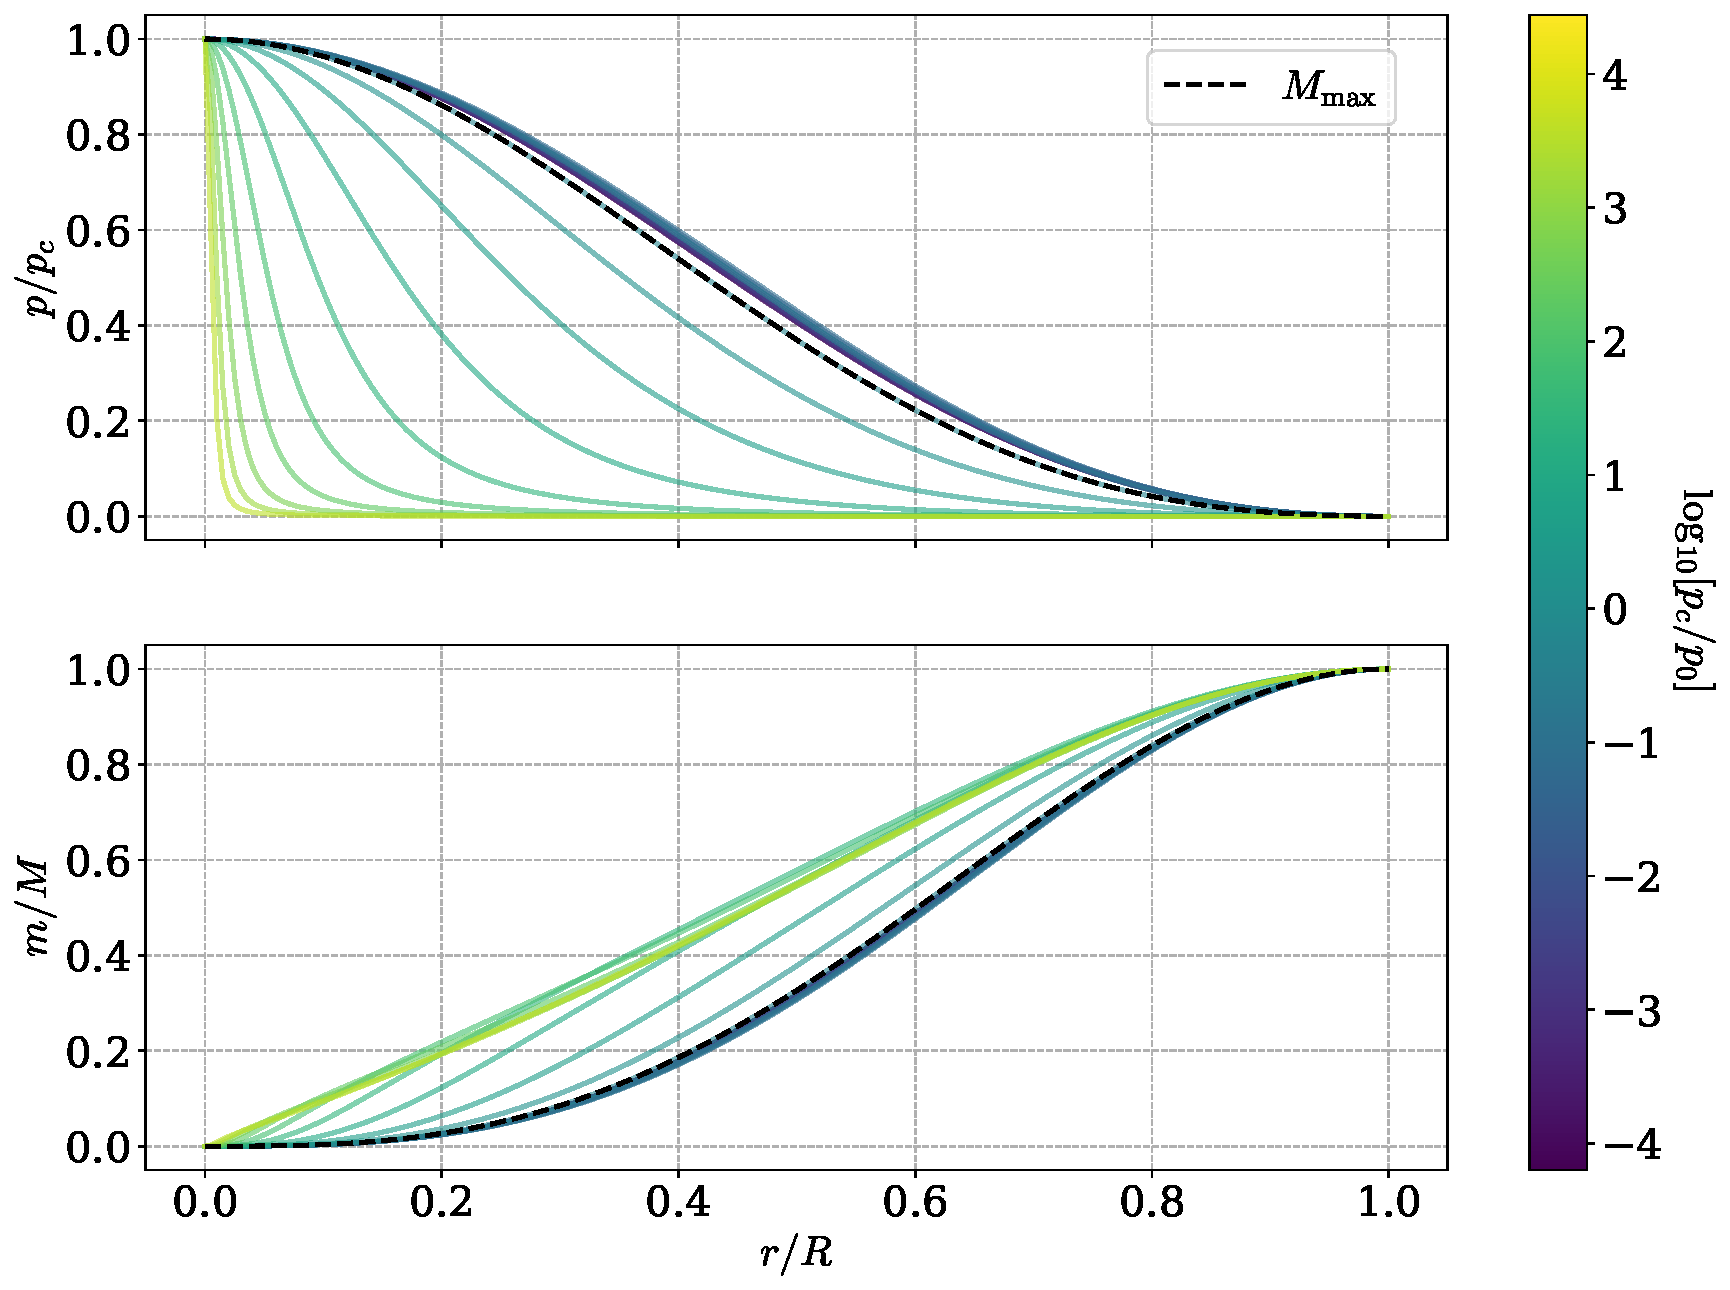
\includegraphics[width=0.8\textwidth]{../scripts/figurer/pion_star/pressure_mass_pion_star.pdf}
    \caption{
    Top: The pressure normalized to the central pressure, as a function of radius, normalized to the stellar radius.
    Bottom: The mass, normalized to the stellar mass, within a radius $r$, normalized to the stellar radius.
    Both plots show a range of stars with different central pressures, indicated by the color.
    The black dashed line corresponds to the star with the largest mass.
    }
    \label{fig: pressure and mass for pion star}
\end{figure}

\begin{figure}[!htb]
    \centering
    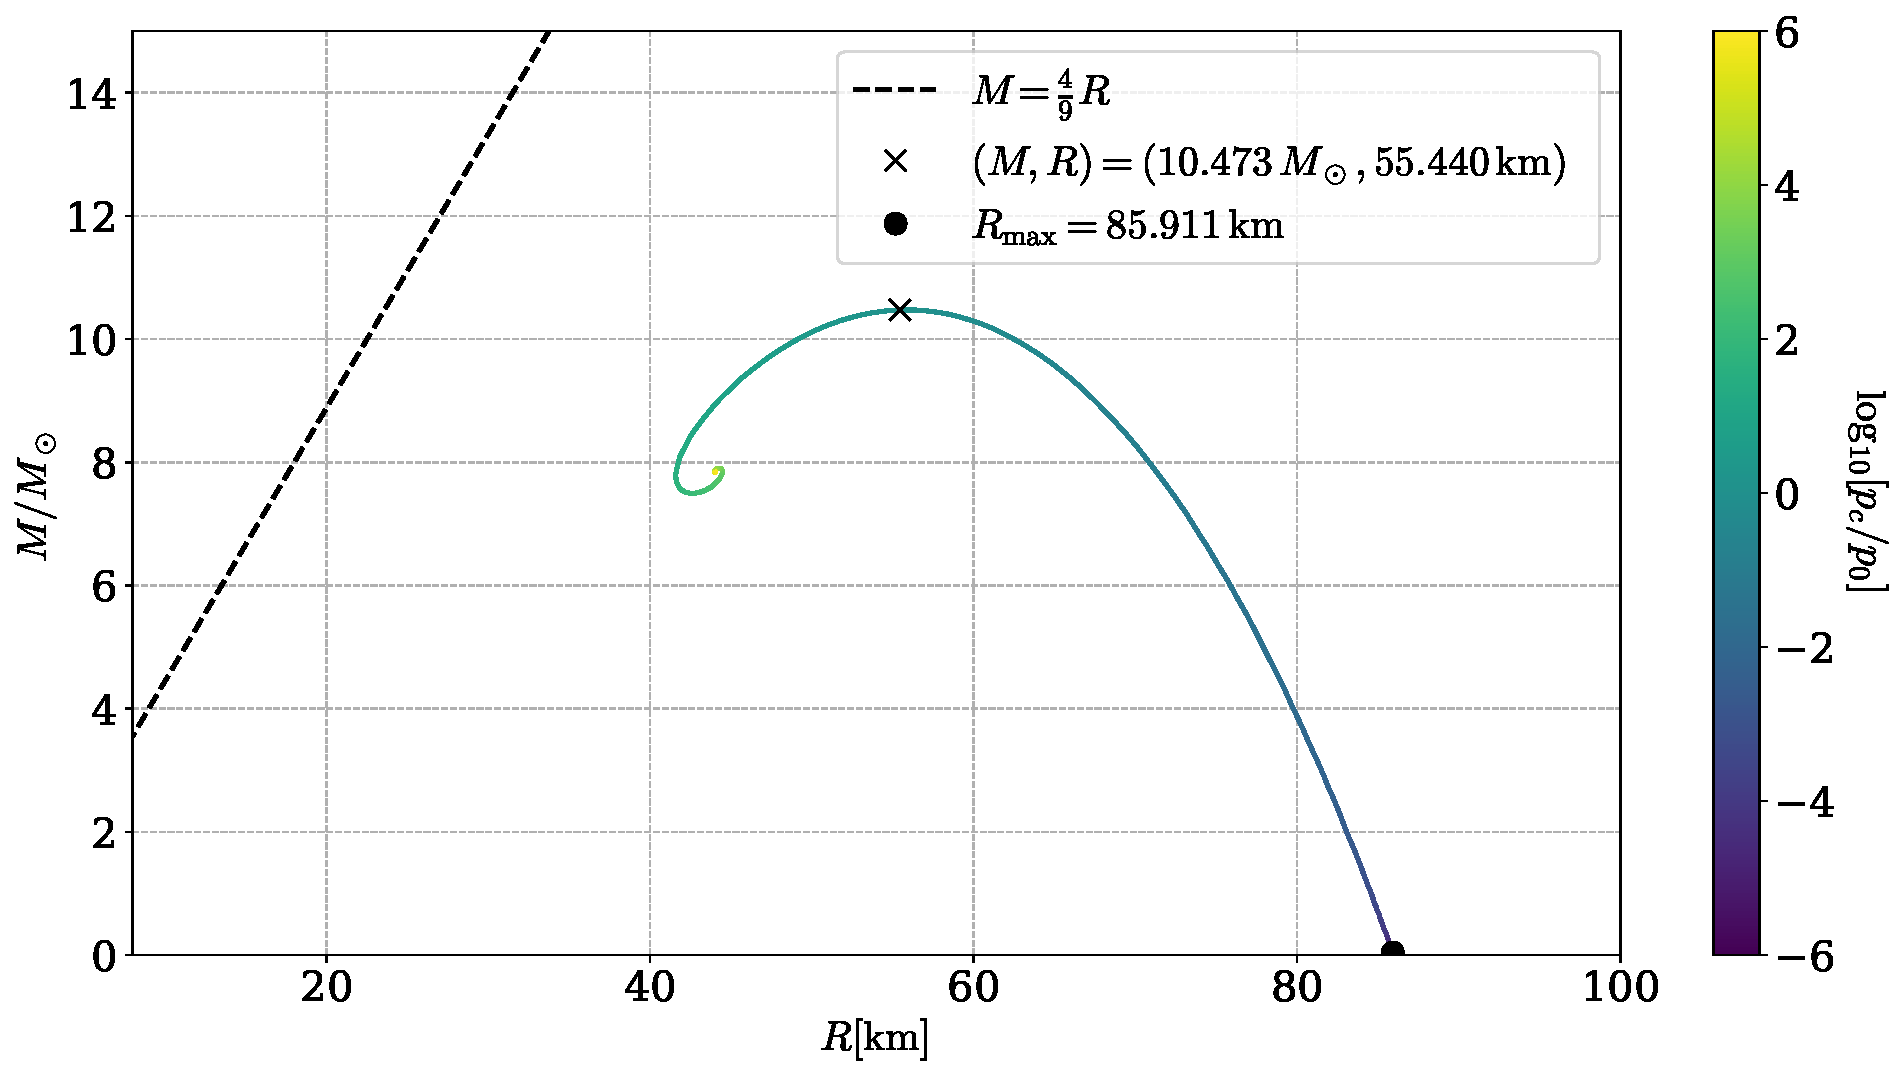
\includegraphics[width=0.85\textwidth]{../scripts/figurer/pion_star/mass_radius_pion_star.pdf}
    \caption{
        The lowest order mass-radius relation of a pion star using two-flavor chiral perturbation theory.
        The mass is given in units of solar masses, while the radius is measured in kilometers.
        This line is parameterized by the central pressure $p_c$ of the star, as indicated by the color gradient.
        The dashed black line indicates the theoretical maximum mass for a given radius, and any configuration above it will collapse to form a black hole.
        }
        \label{fig: mass-radius relation pion star}
\end{figure}

\begin{figure}[!htb]
    \centering
    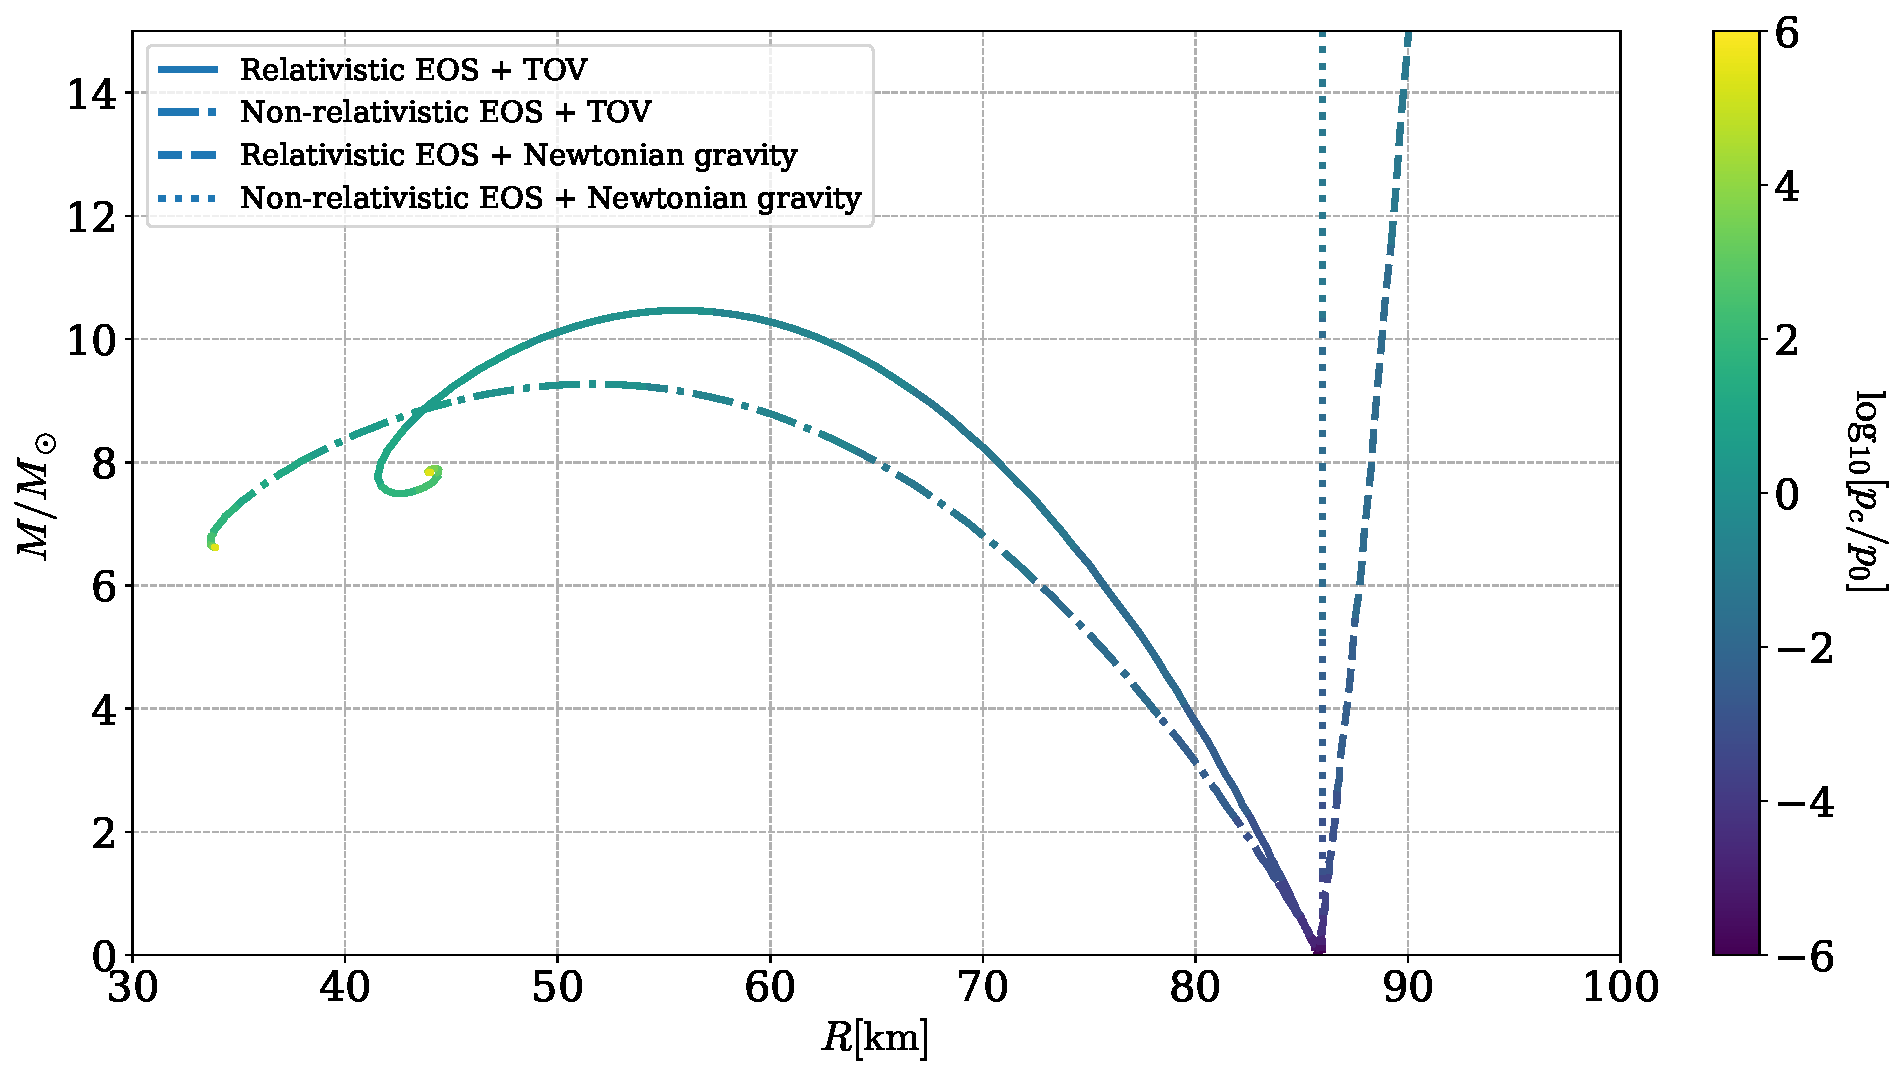
\includegraphics[width=0.85\textwidth]{../scripts/figurer/pion_star/mass_radius_comparison.pdf}
    \caption{
        The mass-radius relationship of the pion star from the full, leading-order equation of state from two-flavor chiral perturbation and the TOV equation, compared with results in various limits.
        }
        \label{fig: mass-radius relation pion star comparison}
\end{figure}



\FloatBarrier
\subsection{Including electromagnetic contributions}

As we found in \autoref{subsection: including electromagnetism lo eos}, the electromagnetic interaction of the pseudoscalar mesons contributes to the equation of state, even at leading order.
\autoref{fig: pressure and energy with EM interaction} shows the pressure and energy density, normalized to their characteristic quantities, as a function of chemical potential above the critical value, normalized to $\bar m$.
\autoref{fig: eos chpt em interaction} shows the equation of state.
The results with and without electromagnetic results are compared.
We see that the inclusion of electromagnetic contributions results in a less stiff equation of state; a given pressure corresponds to a higher energy density when including electromagnetic interactions.

\autoref{fig: mass-radius relation leading order pion star with em interaction} shows the mass-radius reaction of the pion star when the electromagnetic interaction is taken into account.
We see that the shape of the curve has not changed much from our earlier result. 
Both the maximum mass and radius are slightly smaller.
The new result for maximum radius, $R_\text{max} = 80.35 \, \text{km}$, is in excellent agreement with our expectation, \autoref{maximum mass pion star with em interaction}.
The result with and without electromagnetic interaction is compared in \autoref{fig: mass-radius relation comparison}.
As discussed in \autoref{section: cold fermi star}, we expect a stiffer equation of state to correspond to a more massive star, as happens in this case.

\begin{figure}[!htb]
    \centering
    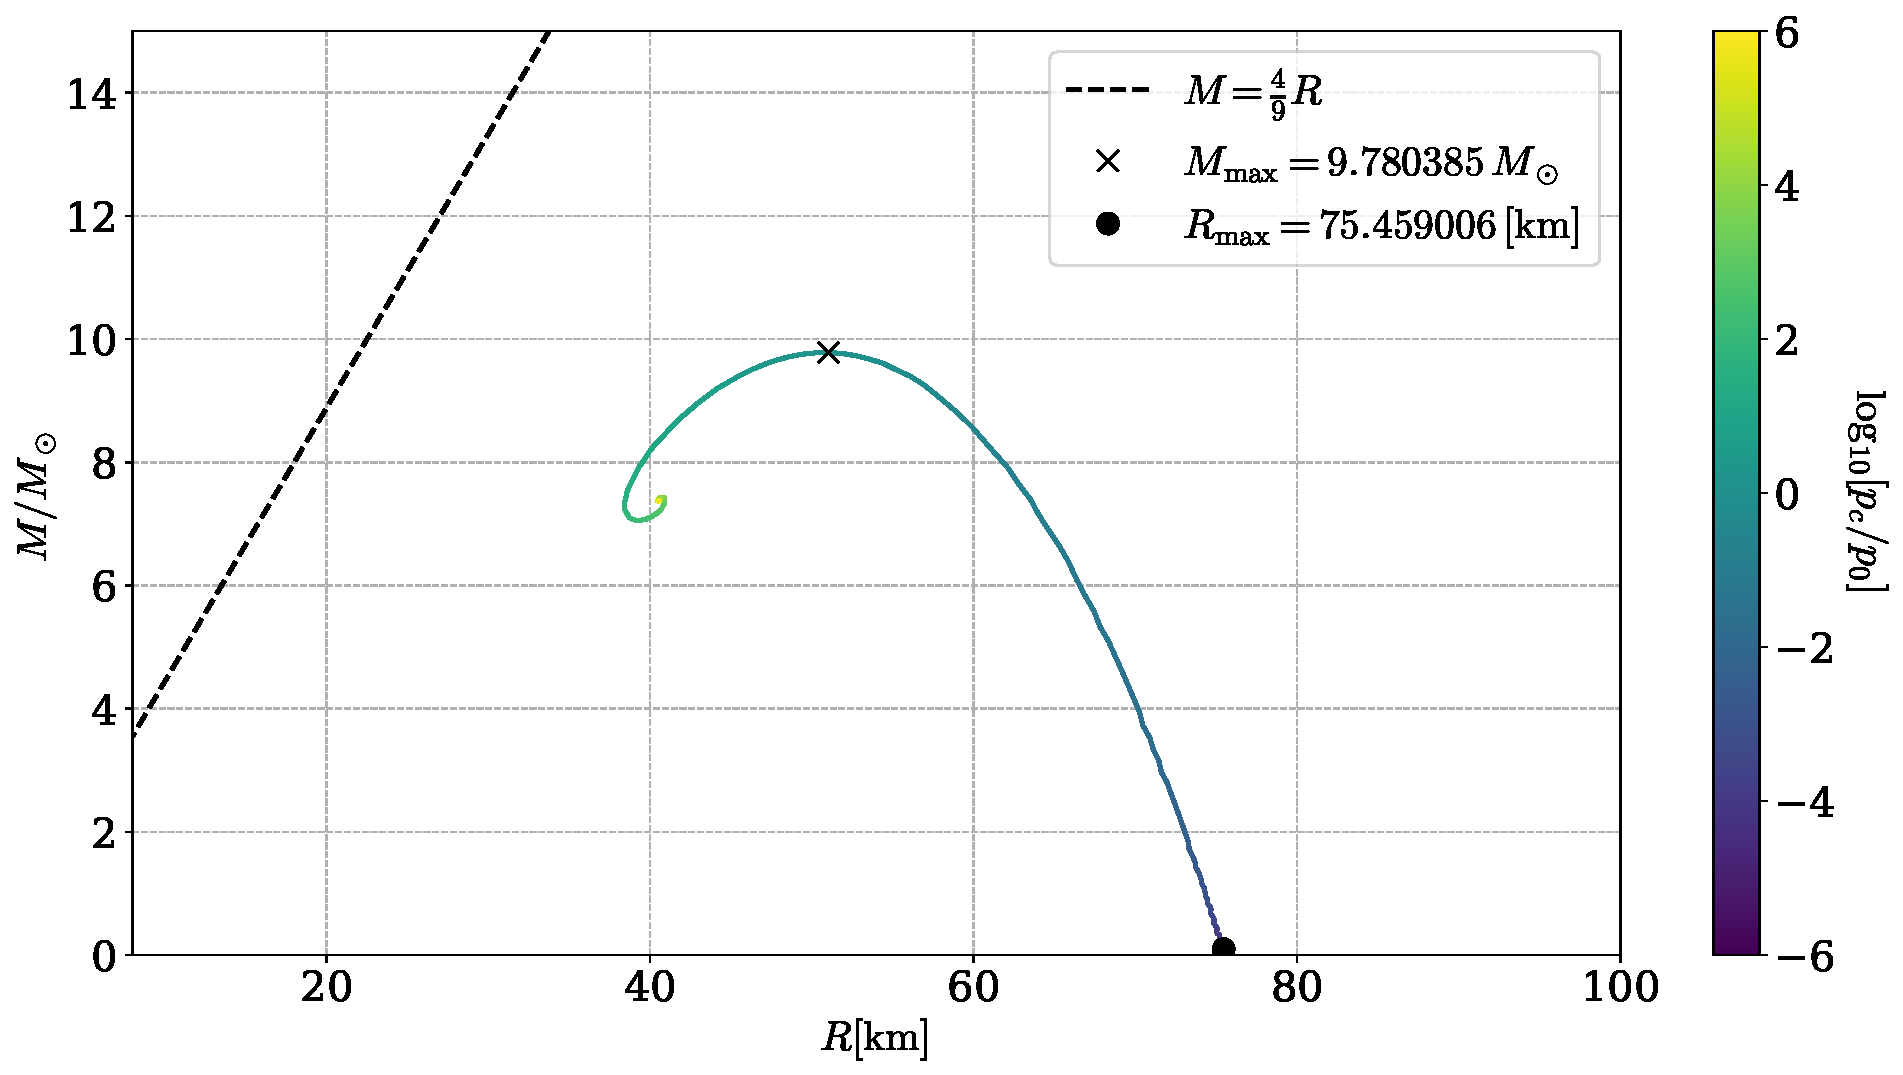
\includegraphics[width=0.85\textwidth]{../scripts/figurer/pion_star/mass_radius_pion_star_EM.pdf}
    \caption{
        The mass-radius relation of a pion star including electromagnetic interactions, parameterized by the logarithm of the central pressure.
        The dashed line shows the absolute limiting mass for a given radius.
        The cross indicates the maximum mass configuration, and the dot the maximum radius configuration.
        The mass is given in units of solar masses, while the radius is in kilometers.
        }
    \label{fig: mass-radius relation leading order pion star with em interaction}
\end{figure}


\begin{figure}[!htb]
    \centering
    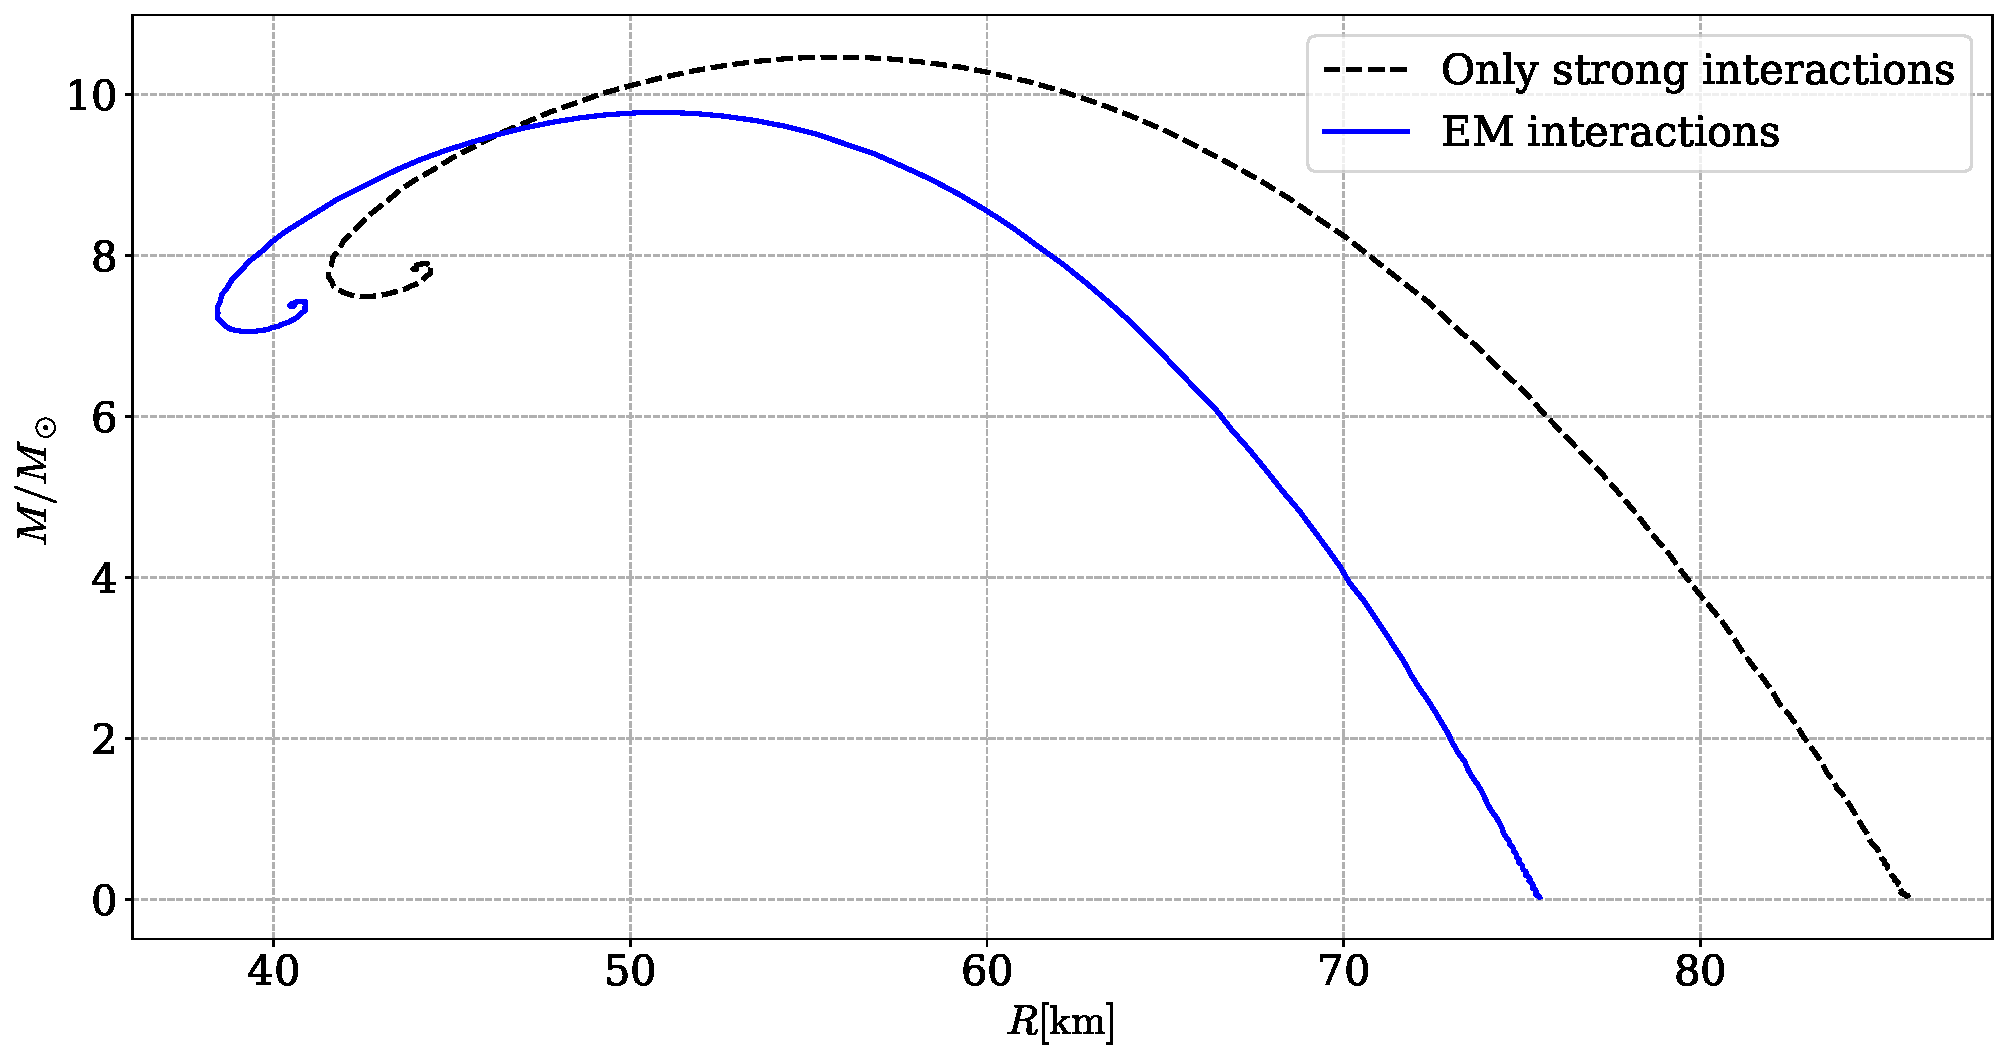
\includegraphics[width=0.8\textwidth]{../scripts/figurer/pion_star/mass_radius_pion_star_compare.pdf}
    \caption{
        The mass-radius relation of pion stars with and without the effects of electromagnetism included.
        The radius is given in kilometers and the mass in units of the solar mass.
        The marked points are the maximum mass and corresponding radius of the stars.
        }
        \label{fig: mass-radius relation comparison}
\end{figure}



\FloatBarrier
\subsection{Charge neutral stars}


We now apply the results from \autoref{section: charge neturality}, where we added a lepton to enforce charge neutrality.
As the electromagnetic force is long-range, we should expect any macroscopic astronomical object to be charge neutral.
First, we apply the system of pions and one charged lepton.
The star with electrons is shown in \autoref{fig: mass-radius relation with electrons}.
We see that this star is much larger than those made of only pions.
This is because the light electrons make the equation of state stiffer at low pressures.
The non-relativistic equation of state is now a polytrope with $\gamma = \frac{5}{3}$, instead of $\gamma = 2$, and there is, therefore, no upper limit on the radius.
The maximum mass is now $238\, M_\odot $, and the corresponding maximum radius is $ 3.11\times 10^4 \,\text{km}$.

The mass-radius relation for a star where the lepton is a muon is shown in \autoref{fig: mass-radius relation with muons}.
This has a similar form to that where the lepton was the electron, only smaller and lighter, as the equation of state, in this case, is less stiff.
The maximum mass is now $18.6\, M_\odot $, and the corresponding maximum radius is $ 262 \,\text{km}$.

\begin{figure}[!htb]
    \centering
    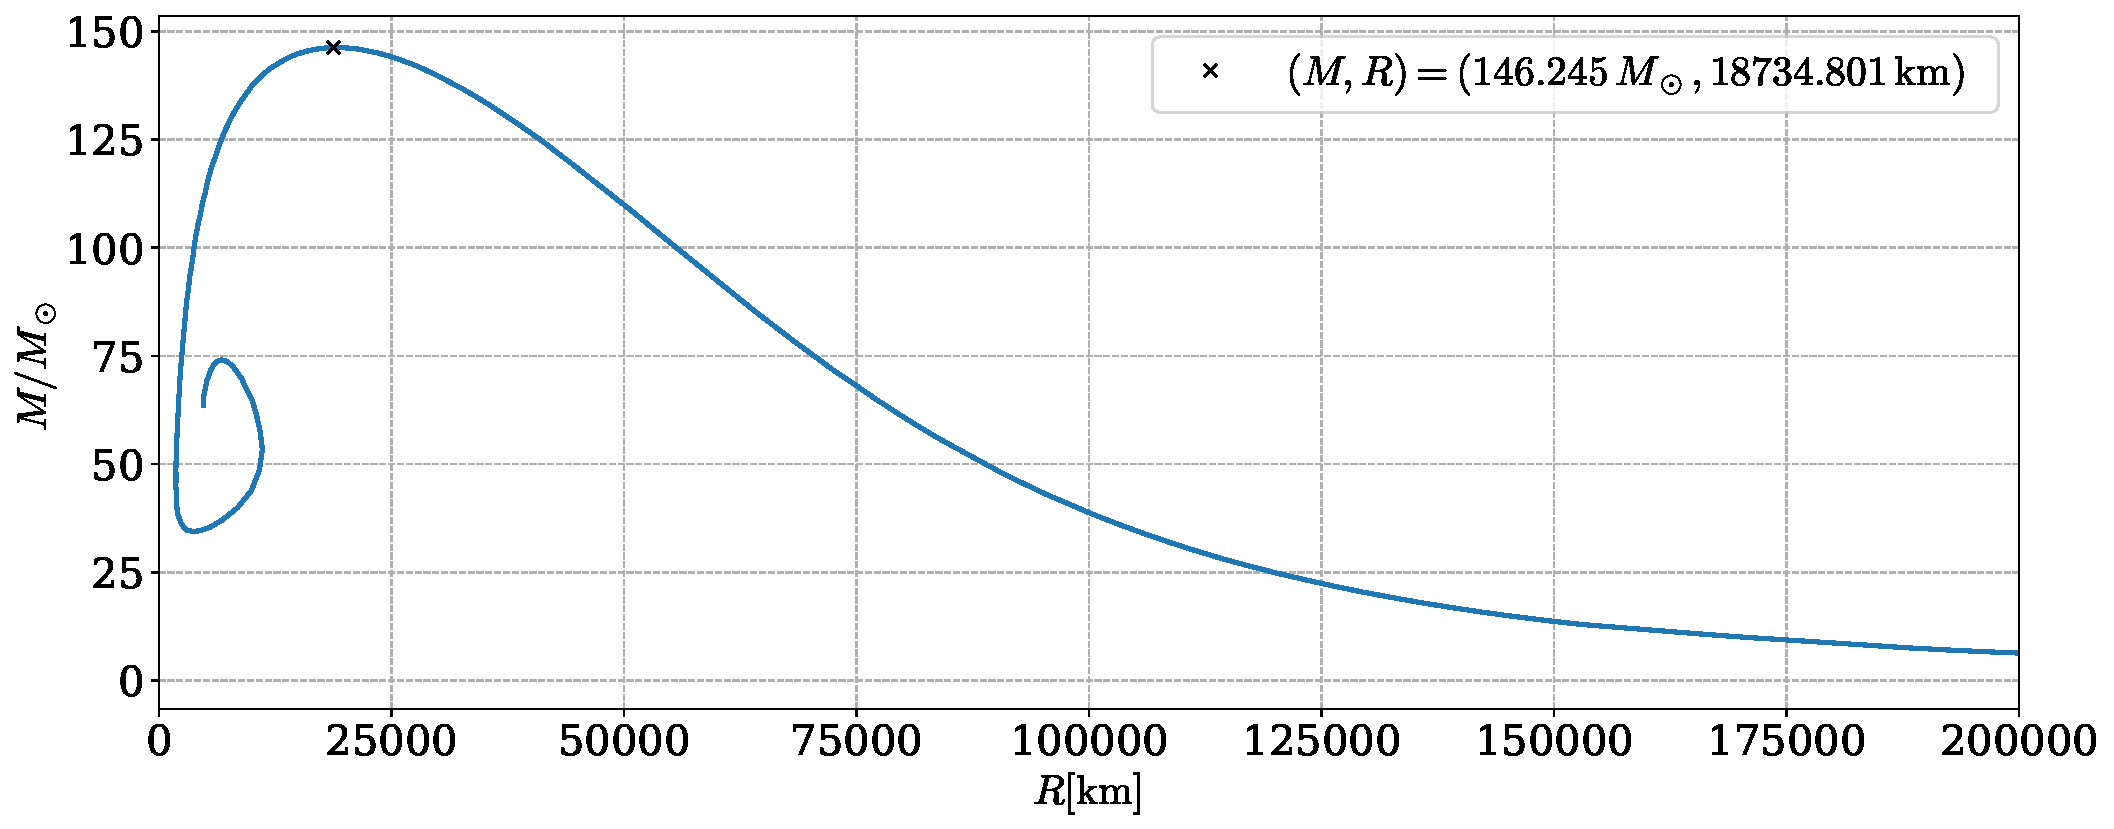
\includegraphics[width=\textwidth]{../scripts/figurer/pion_star/mass_radius__e.pdf}
    \caption{
        The mass-radius relation of pion stars with electrons enforcing charge neutrality.
        The radius is given in kilometers and the mass in units of solar masses.
        }
        \label{fig: mass-radius relation with electrons}
\end{figure}

\begin{figure}[!htb]
    \centering
    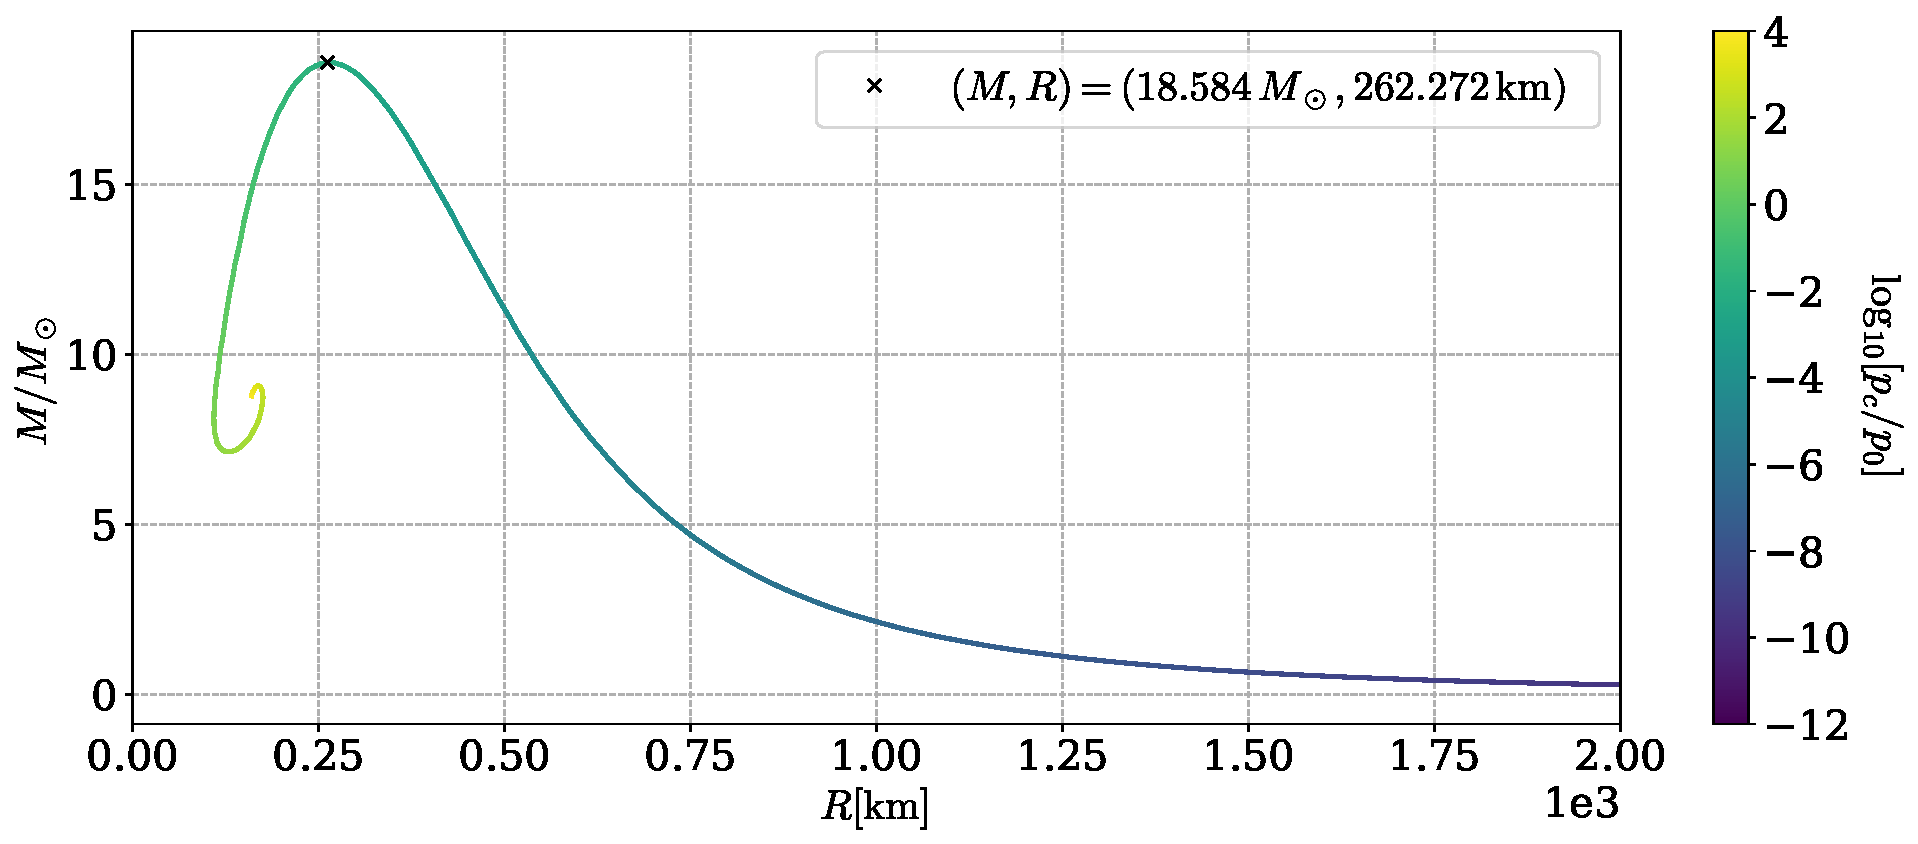
\includegraphics[width=\textwidth]{../scripts/figurer/pion_star/mass_radius__mu.pdf}
    \caption{
        The mass-radius relation of pion stars, including leptons to enforce charge neutrality, is compared with pion stars of only pions.
        The radius is given in kilometers and the mass in units of solar masses.
        }
        \label{fig: mass-radius relation with muons}
\end{figure}



\subsection{Neutrinos}

In \autoref{subsection: neutrinos}, we found the equation of state when including neutrinos in addition to charged leptons and the decay of pions due to the weak force.
In this case, the pressure and energy density do not vanish as the isospin density vanishes, but rather as $p = p_\text{min}>0$ as defined in \autoref{p min}
This is due to the contribution of neutrinos.
We therefore define the stellar radius $R$ by $p(R) = p_\text{min}$, where the pion condensate vanishes.
Such a star will therefore have an atmosphere of ultrarelativistic neutrinos.
For $p < p_\text{min}$, the equation of state is that of massless fermions and will therefore not have a finite radius.
There is a $p+u$-term on the right-hand side of the TOV equation, \autoref{TOV}.
When we defined the stellar radius by $p(R) = 0$, this factor vanishes as we approach the surface of the star, while now $p+u \geq 4 p_\text{min}$.
Close to the surface, the pressure will therefore fall faster, as a consequence of $p_\text{min}>0$.
The resulting mass-radius relation is shown in \autoref{fig: mass radius neutrino}.
We see that, in contrast to the earlier results, both the mass and radius approach zero as $p_c \rightarrow p_\text{min}$.


\begin{figure}[!htb]
    \centering
    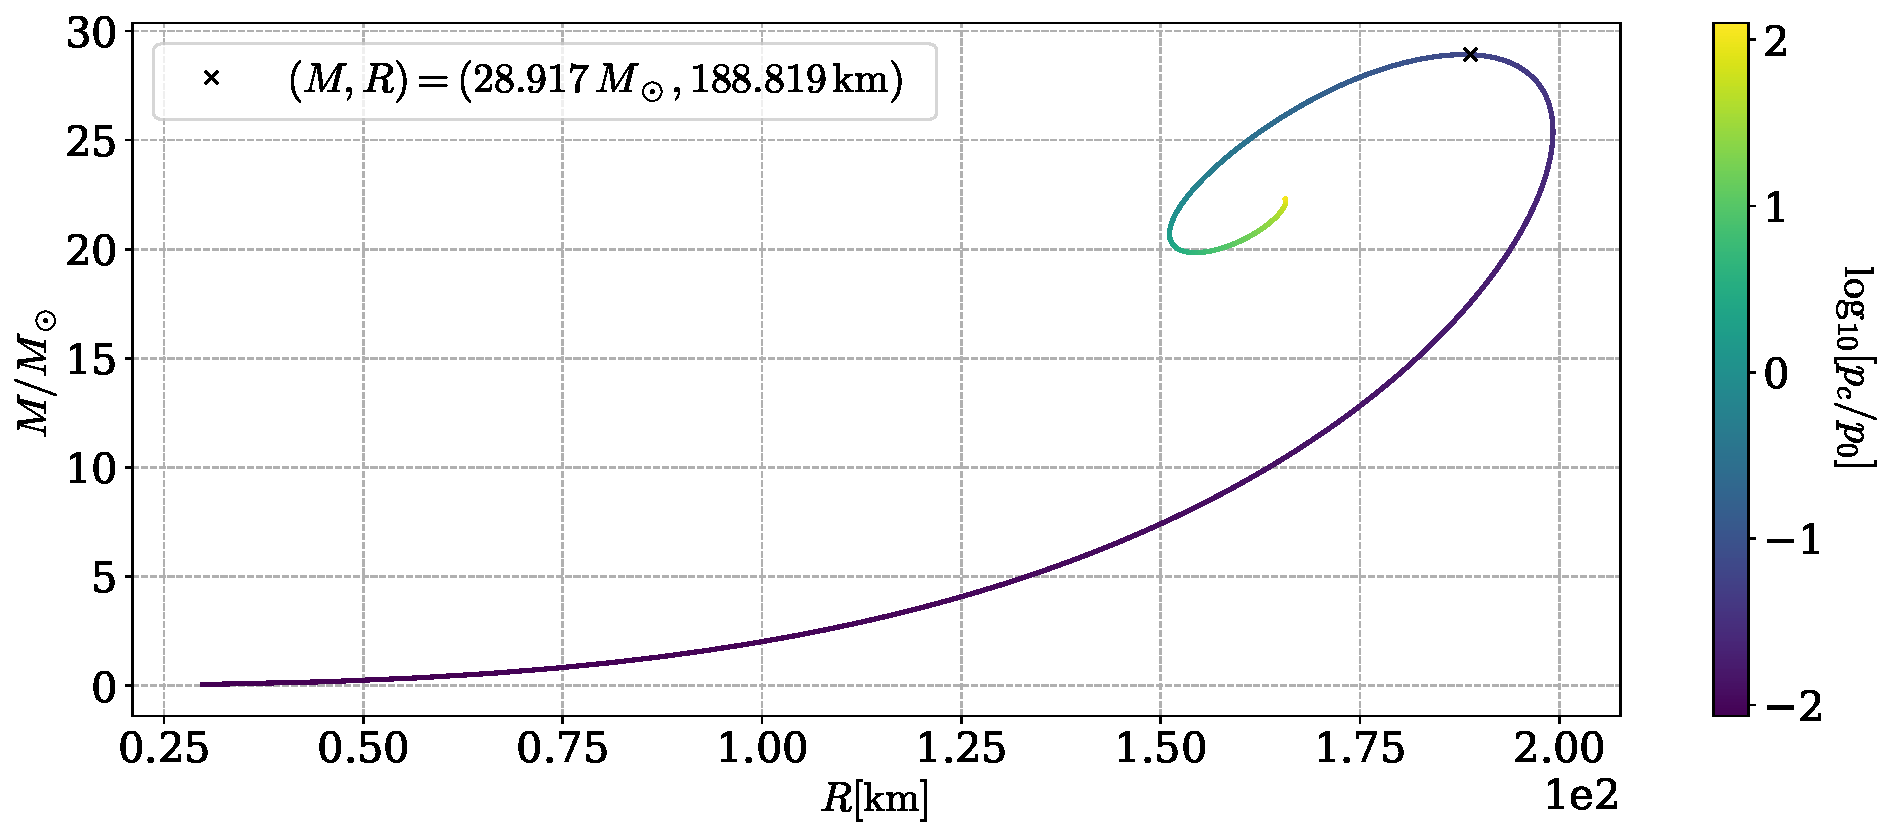
\includegraphics[width=\textwidth]{../scripts/figurer/pion_star/mass_radius_neutrino.pdf}
    \caption{
        The mass-radius relation of pion stars, including leptons and neutrinos in equilibrium.
        The radius is given in kilometers and the mass in units of solar masses.
        }
        \label{fig: mass radius neutrino}
\end{figure}

In \autoref{fig: light stars}, the pion stars including charged leptons and neutrinos are compared to a family of stars with $u = 3p$ but different values for $p_\text{min}$.
We see that the mass-radius relation of the pion star closely resembles that of such a star and that the mass-radius relationship, therefore, is mostly set by $p_\text{min}$.


\begin{figure}[!htb]
    \centering
    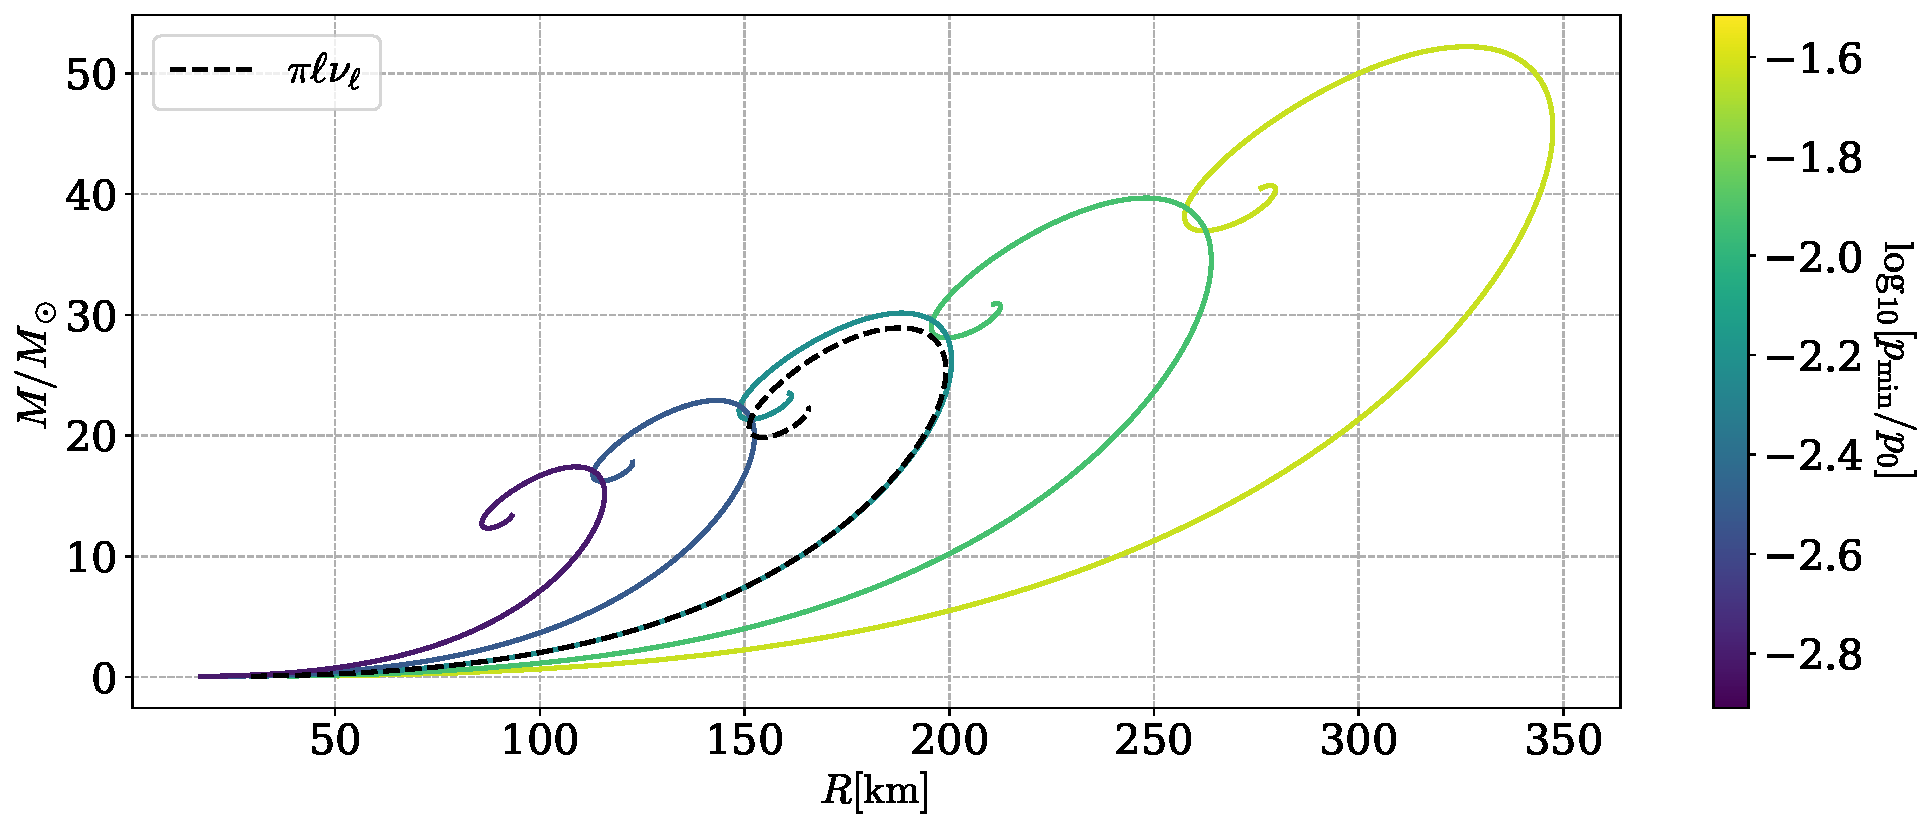
\includegraphics[width=\textwidth]{../scripts/figurer/pion_star/mass_radius_light.pdf}
    \caption{Stars with equation of state $u = 3p$ but different values for $p_\text{min}>0$ is compared to the pion star with charged leptons and neutrinos.}
    \label{fig: light stars}
\end{figure}


\subsection{NLO pion star}

We now use the next-to-leading order results for the pure pion condensate, which we found in \autoref{section: nlo thermodynamics}.
The mass-radius relationship, in this case, is shown in \autoref{fig: mass-radius relation nlo}.
The maximum mass is $M_\text{max} = 9.94\, M_0$, and the corresponding radius is $R = 54.09\,\text{km}$.
In \autoref{fig: mass-radius relation compare nlo}, we compare the leading order and next-to-leading order mass-radius relations.
The results are similar, however, the next-to-leading order star is smaller and less massive, as is expected for a less stiff equation of state.

\begin{figure}[!htb]
    \centering
    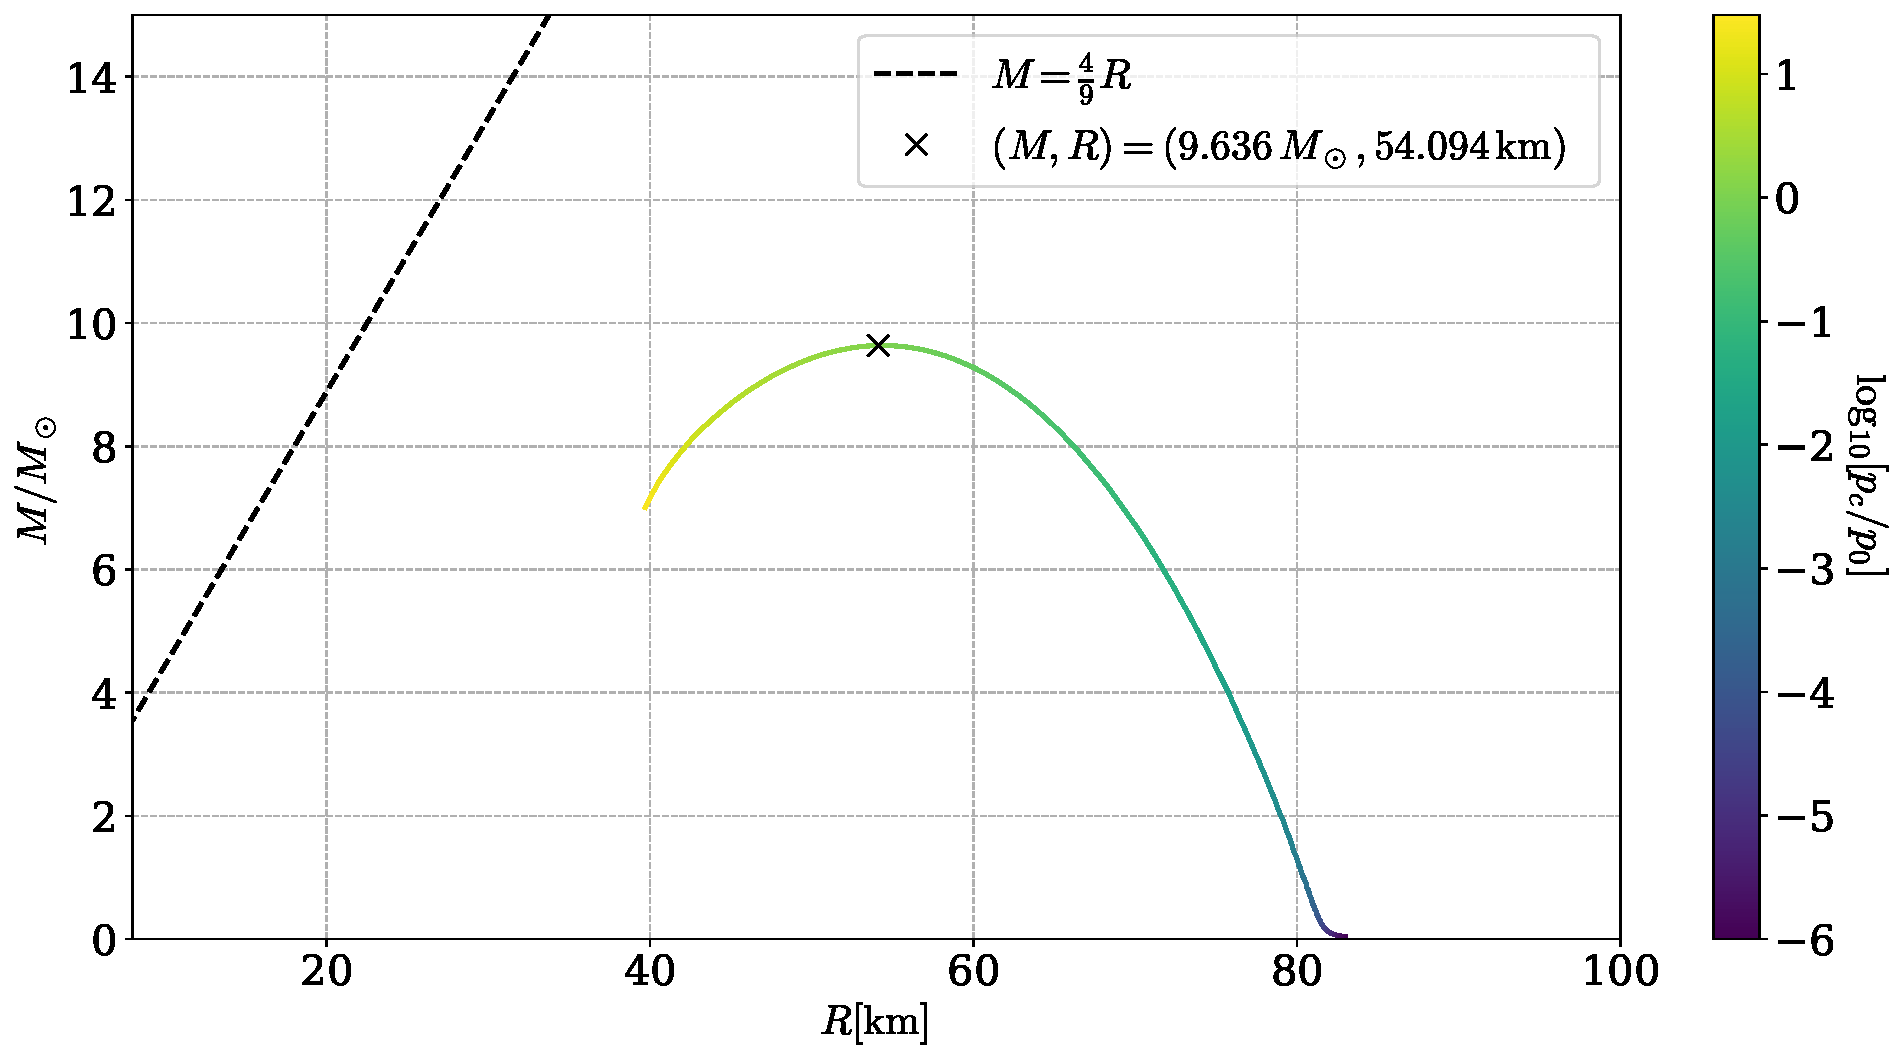
\includegraphics[width=\textwidth]{../scripts/figurer/pion_star/mass_radius_pion_star_nlo.pdf}
    \caption{The mass-radius relation of a pion star with the next-to-leading order equation of state.}
    \label{fig: mass-radius relation nlo}
\end{figure}

\begin{figure}[!htb]
    \centering
    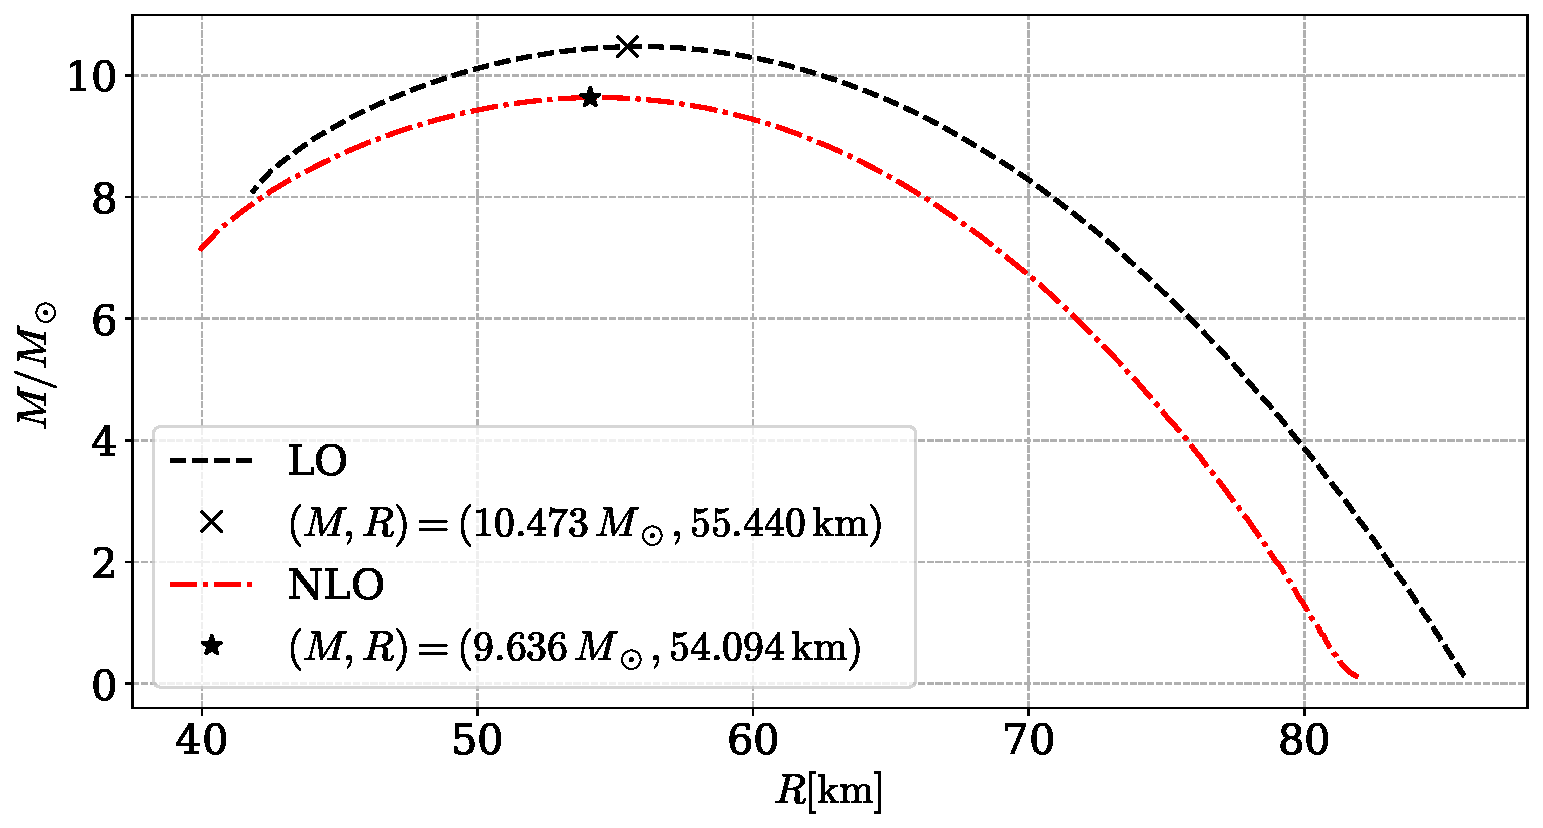
\includegraphics[width=\textwidth]{../scripts/figurer/pion_star/mass_compare_order.pdf}
    \caption{
        The mass-radius relation of a pion star using the leading and next-to-leading order equation of state is compared. 
        The mass is given in solar masses and the radius in kilometers.}
    \label{fig: mass-radius relation compare nlo}
\end{figure}



\section{Comparison and key values}



All results are compared in \autoref{fig: mass-radius relation with leptons}.

\begin{figure}[!htb]
    \centering
    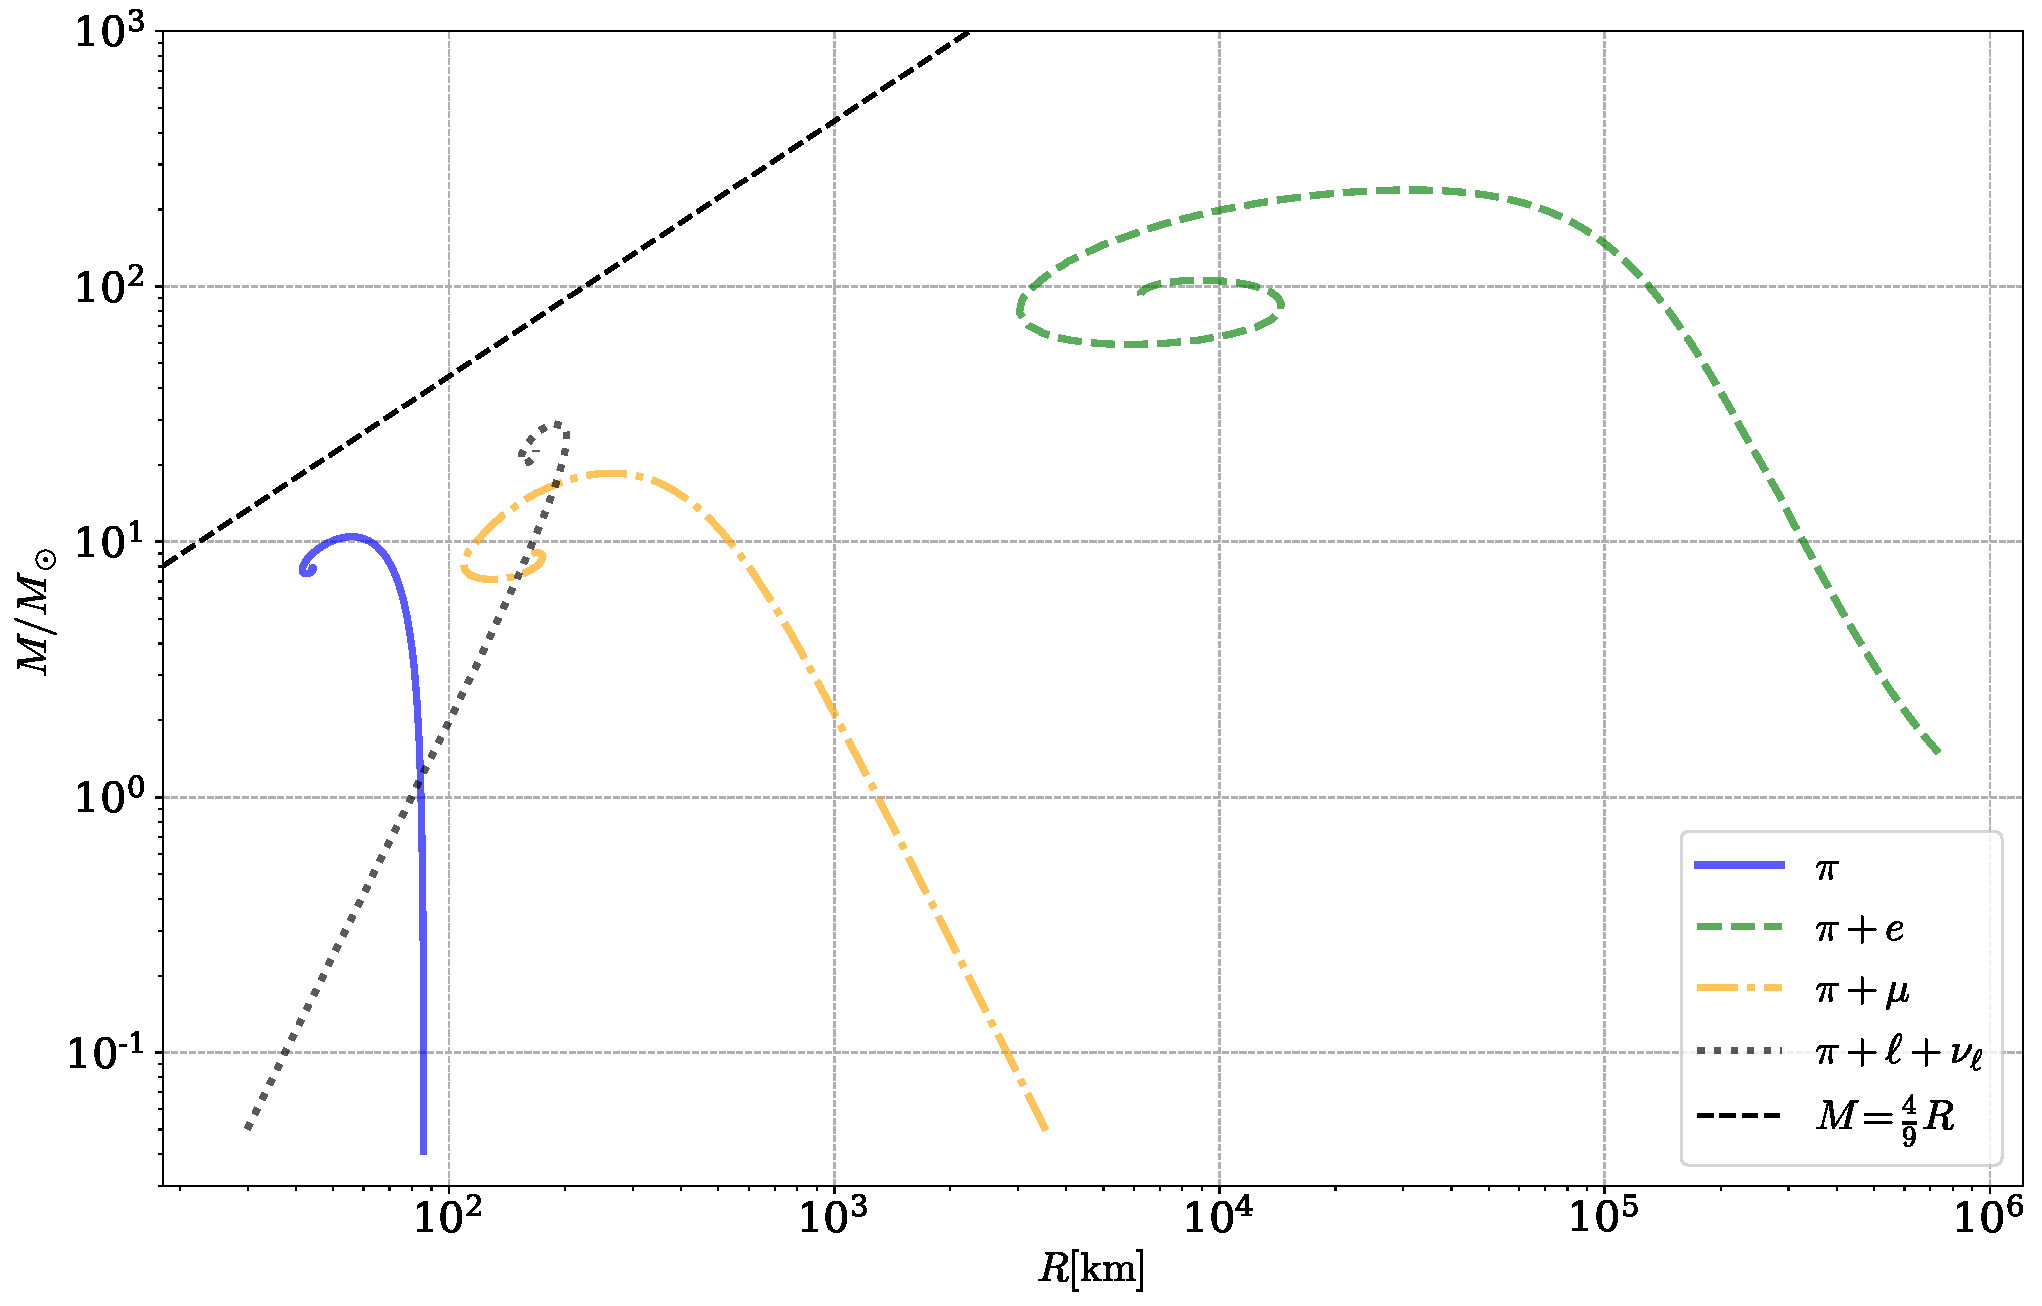
\includegraphics[width=\textwidth]{../scripts/figurer/pion_star/mass_radius_all.pdf}
    \caption{
        The mass-radius relation of pion stars, including leptons to enforce charge neutrality, is compared with pion stars of only pions.
        The radius is given in kilometers and the mass in units of solar masses.
        }
        \label{fig: mass-radius relation with leptons}
\end{figure}


Key values for each system are shown in \autoref{table: key values}.


\begin{table}[!htb]
    \centering
    \caption{The values of various quantities for the maximum mass stars}
    \label{table: key values}
    \begin{tabular}{c  c  c  c  c c c}
        \hline \hline
        system & $M_\text{max}/M_\odot$ & $R / \text{km}$ & 
        $u/u_0$ & $p/u_0$ & $\mu_I/m_\pi-1$ & $\mu_\ell/m_\ell-1$ \\
        \hline
        $\pi\,\, \text{LO}$& 10.47 & 55.38 & 2.864 & 1.318 & 0.8461& \\
        $\pi\, \text{NLO}$& 9.04 & 54.09 & 3.020 & 1.139 & 0.9256 & \\
        $\pi\,\,\text{EM}$& 10.11 & 53.58 & 2.930 & 1.318 & 0.8463 & \\
        $\pi + e$& 283.8 & 3.171$\times10^4$ & 
        2.550$\times10^{-6}$ & 1.995$\times10^{-8}$ & 
        6.222$\times10^{-6}$ & \\
        $\pi + \mu$& 18.58 & 262.3 & 
        0.1411 & 1.202$\times 10^{-2}$ &
        1.732$\times10^{-2}$& \\
        $\pi + \ell + \nu_\ell$& 28.92 & 188.8 &
        0.2262  & 6.847$\times 10^{-2}$ &
        5.264$\times10^{-3}$& \\
        \hline
    \end{tabular}
\end{table}



\subsection{Comparison with numerical results}

In \autocite{brandtNewClassCompact2018}, \citeauthor{brandtNewClassCompact2018} used the equation of state obtained by QCD lattice methods to obtain mass-radius relations for pion stars, with and without leptons for charge neutrality.
Their results are compared with ours in  \autoref{fig: brandt mass-radius}.


\begin{figure}[!htb]
    \centering
    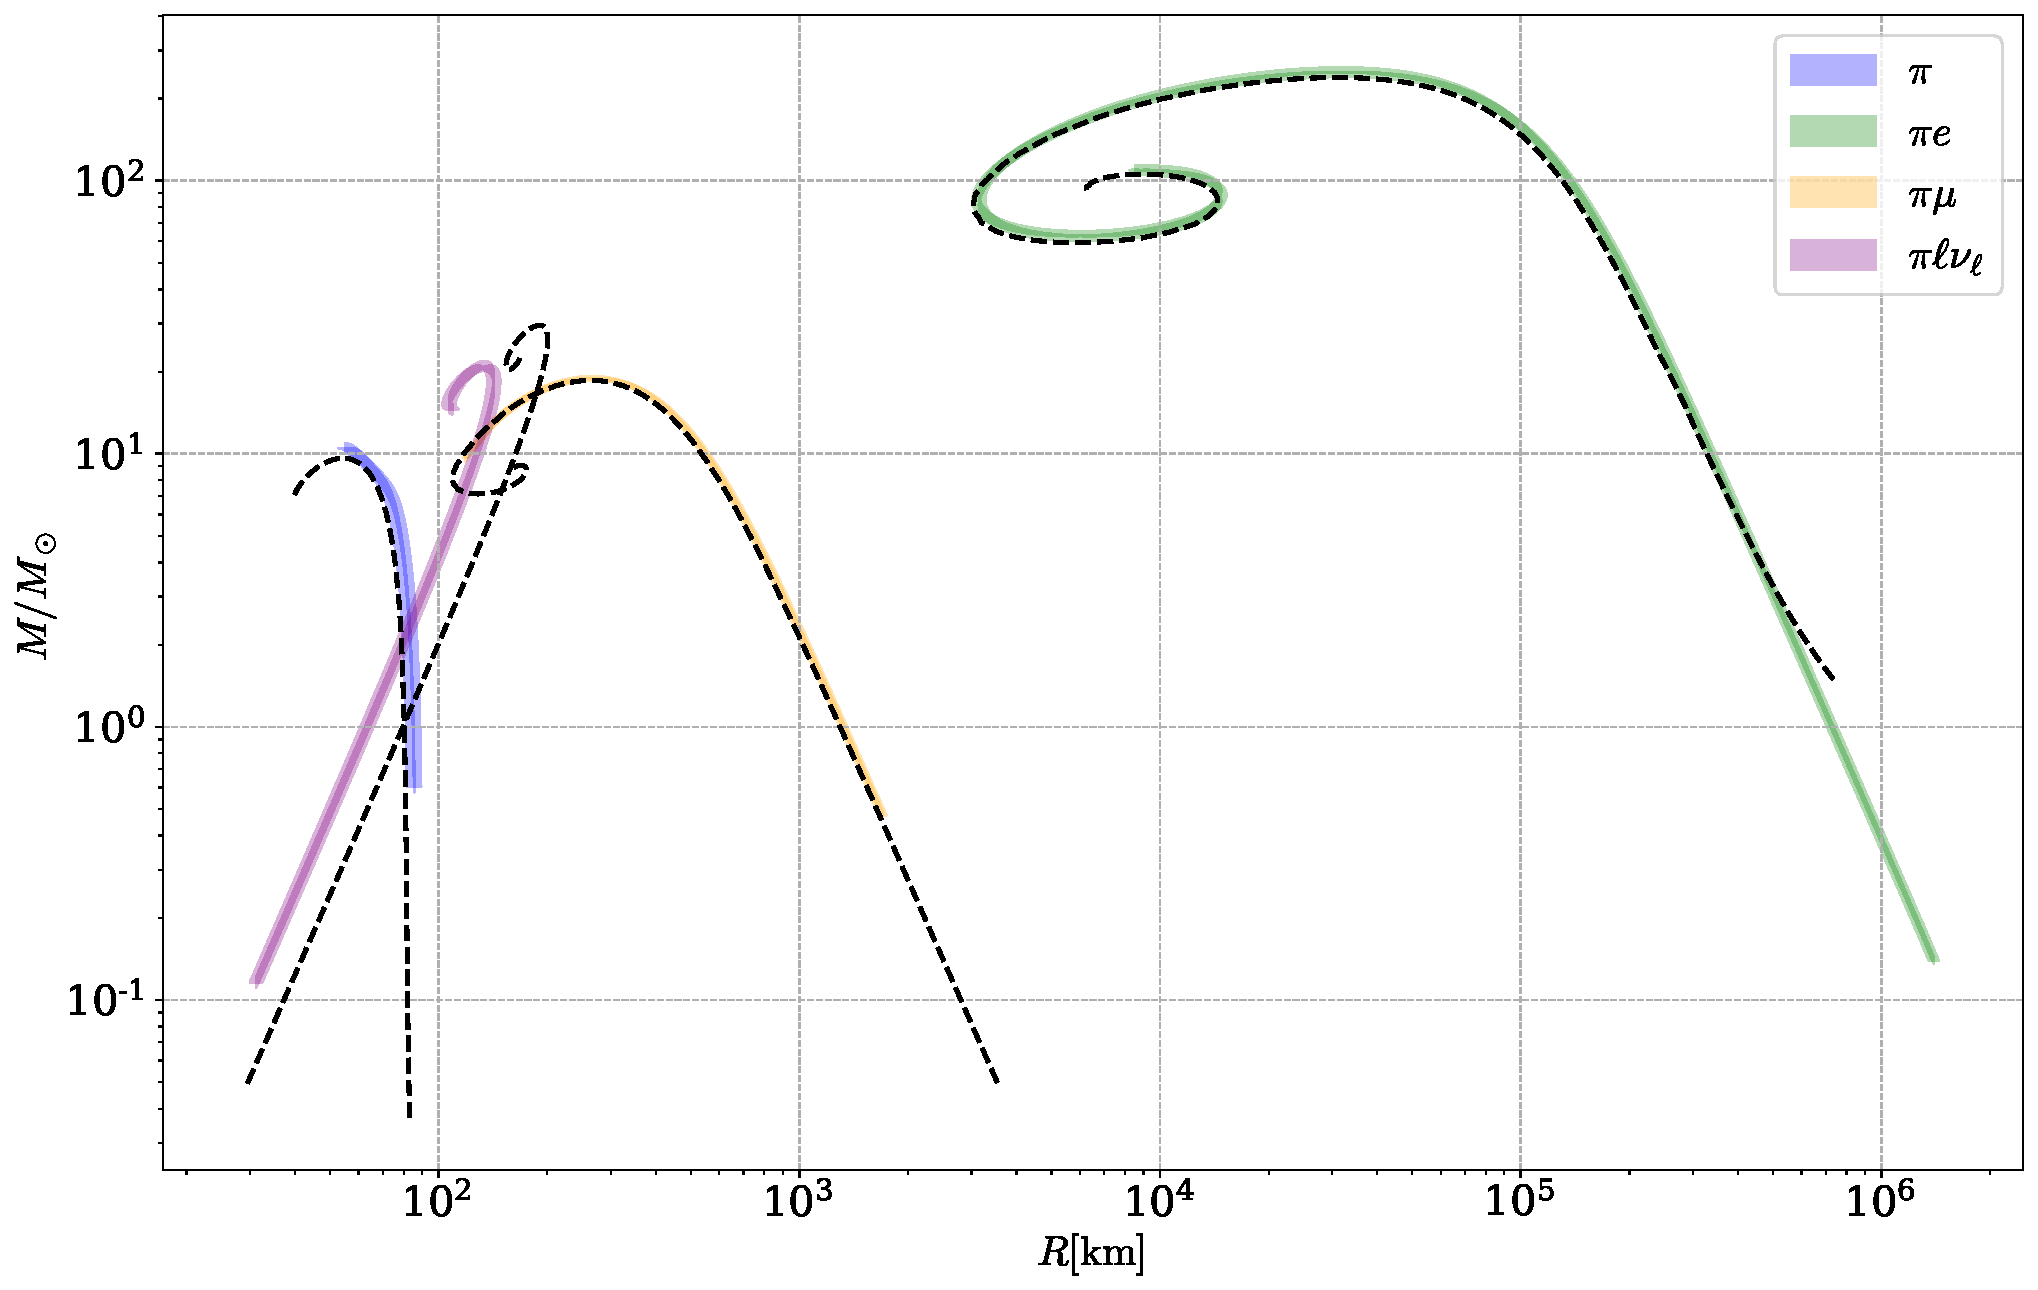
\includegraphics[width=\textwidth]{../scripts/figurer/pion_star/mass_radius_brandt_all.pdf}
    \caption{
        The mass-radius relations for pion stars, with and without leptons included.
        The results of \citeauthor{brandtNewClassCompact2018}, solid color, are compared with our results, dashed lines.
        The result of \citeauthor{brandtNewClassCompact2018} incorporate statistical and systematic uncertainty in both $R$ and $M$ in the width of the lines.
        The radius is in units of $\text{km}$, while mass are in solar masses, $M_\odot$.
    }
    \label{fig: brandt mass-radius}
\end{figure}



    \appendix

    \chapter[Appendix A]{}
    \section{Algebra bases}
\label{section: algebra bases}

\subsection{Pauli matrices}
\label{subsection: Pauli matrices}

The Pauli matrices are
\begin{align}
    \tau_1 = 
    \begin{pmatrix}
        0 & 1 \\
        1 & 0 \\
    \end{pmatrix}
    , \quad 
    \tau_2 = 
    \begin{pmatrix}
        0 & -i \\
        i & 0 \\
    \end{pmatrix}, \quad 
    \tau_3 = 
    \begin{pmatrix}
        1 & 0 \\
        0 & -1 \\
    \end{pmatrix}.
\end{align}
They obey
\begin{align}
    [\tau_a, \tau_b] &= 2 i \varepsilon_{abc}\tau_c, \\
    \{\tau_a,\tau_b\} &= 2\delta_{ab} \one, \\
    \Tr{\tau_a} &= 0, \\
    \Tr{\tau_a \tau_b} &= 2 \delta_{ab}, \\
    \Tr{\tau_a\tau_b\tau_c\tau_d} 
    & = 2 (\delta_{ab}\delta_{cd} - \delta_{ac}\delta_{cb} + \delta_{ad}\delta_{cb}).
\end{align}
Together with the identity matrix $\one$, the Pauli matrices form a basis for the vector space of all 2-by-2 matrices.
An arbitrary 2-by-2 matrix $M$ may be written
\begin{equation}
    \label{2-by-2 matrix decomp}
    M = M_0 \one + M_a \tau_a, \quad 
    M_0 = \frac{1}{2} \Tr{M}, \,\, M_a = \frac{1}{2} \Tr{\tau_a M}.
\end{equation}


\subsection{Gell-Mann matrices}
\label{subsection: gell-mann matrices}


The Gell-Mann matrices are
%
\begin{align}
    \lambda_1
    & = 
    \begin{pmatrix}
        0 & 1 & 0 \\
        1 & 0 & 0 \\
        0 & 0 & 0
    \end{pmatrix},\,
    \lambda_2
    = 
    \begin{pmatrix}
        0 & -i & 0 \\
        i & 0 & 0 \\
        0 & 0 & 0
    \end{pmatrix},\,
    \lambda_3
    = 
    \begin{pmatrix}
        1 & 0 & 0 \\
        0 & -1 & 0 \\
        0 & 0 & 0
    \end{pmatrix},\\
    \lambda_4
    & = 
    \begin{pmatrix}
        0 & 0 & 1 \\
        0 & 0 & 0 \\
        1 & 0 & 0
    \end{pmatrix},\,
    \lambda_5
    = 
    \begin{pmatrix}
        0 & 0 & -i \\
        0 & 0 & 0 \\
        i & 0 & 0
    \end{pmatrix},\,
    \lambda_6
    = 
    \begin{pmatrix}
        0 & 0 & 0 \\
        0 & 0 & 1 \\
        0 & 1 & 0
    \end{pmatrix},\\
    \lambda_7
    & = 
    \begin{pmatrix}
        0 & 0 & 0 \\
        0 & 0 & -i \\
        0 & i & 0
    \end{pmatrix},\,
    \lambda_8
    =  \frac{1}{\sqrt 3}
    \begin{pmatrix}
        1 & 0 & 0 \\
        0 & 1 & 0 \\
        0 & 0 & -2
    \end{pmatrix}.
\end{align}
%
They obey
%
\begin{align}
    [\lambda_a, \lambda_b] & = 2if^{abc} \lambda_c, \\
    \{\lambda_a, \lambda_b\} & = \frac{4}{3}\one \delta_{ab} + 2d_{abc} \lambda_c, \\
    \Tr{\lambda_a} & = 0, \\
    \Tr{\lambda_a \lambda_b} &= 2 \delta_{ab}, \\
    \Tr{\lambda_a \lambda_b \lambda_c \lambda_d} 
    &= \frac{4}{3} \delta_{ab}\delta_{cd} + 2 (d_{abe} + if_{abe})(d_{cde} + if_{cde}).
\end{align}
%
where
%
\begin{equation}
    f_{abc} = -\frac{i}{4}\Tr{\lambda_a[\lambda_b, \lambda_c]}, 
    \quad
    d_{abc} = -\frac{i}{4}\Tr{\lambda_a\{\lambda_b, \lambda_c\}}.
\end{equation}
%
where the non-zero elements of $f_{abc}$ and $d_{abc}$ are
%
\begin{align}
    f_{123} &= 1, \quad 
    f_{147} = f_{246} = f_{257} = f_{345} = -f_{156} =  f_{367} = \frac{1}{2}, \quad
    f_{458} = f_{678} = \frac{\sqrt 3}{2}, \\
    d_{146} &= d_{157} = d_{256} = -d_{247} = d_{355} = - d_{366} = -d_{377} = \frac{1}{2} \\
    d_{118}& = d_{228} = d_{338} = - d_{888} = \frac{1}{\sqrt 3}, \quad
    d_{448} = d_{558} = d_{668} = d_{778} = - \frac{1}{2 \sqrt 3},
\end{align}
%
or a permutation of the indices.
The indices of $f$ are totally antisymmetric, while those of $d$ are totally symmetric~\autocite{borodulinCORECOmpendiumRElations2017}.




\subsection{Gamma matrices}
\label{subsection: gamma matrices}

The gamma matrices $\gamma^\mu$, $\mu \in \{0, 1, 2, 3\}$, obey
%
\begin{align}
    \{\gamma^\mu,\gamma^\nu\} = 2 g^{\mu \nu} \one,\\
    {\gamma^0}^\dagger = \gamma^0, \quad {\gamma^i}^\dagger = - \gamma^i.
\end{align}
%
These matrices, together with
%
\begin{align}
    \sigma^{\mu\nu} &= \frac{1}{2} [\gamma^\mu, \gamma^\mu], \\ 
    \gamma_A^\mu &= \gamma^\mu \gamma^5, \\
     \gamma^5 
    &= \frac{i}{4!}\epsilon_{\mu \nu \rho \sigma} \gamma^{\mu}\gamma^{\nu}\gamma^{\rho}\gamma^{\sigma},
\end{align}
%
form the Clifford algebra $\text{Cl}_{1,3}$, also known as the \emph{space-time algebra}.
The subscripts $(1, 3)$ denotes the signature of the metric.
The ``fifth $\gamma$-matrix'', which can be expressed as $\gamma^5 = \gamma^0\gamma^1\gamma^2\gamma^3$, obey
%
\begin{equation}
    \{\gamma^5,\gamma^\mu\} = 0, \quad (\gamma^5)^2 = \one.
\end{equation}


The Euclidian counterpart of the space-time algebra, $\text{Cl}_4$, is defined by the ``Euclidian gamma matrices'', which obey
%
\begin{equation}
    \{\tilde \gamma_a, \tilde \gamma_b\} = 2 \delta_{ab}\one.
\end{equation}
%
These can be related to the regular Minkowski-matrices by
%
\begin{equation}
    \tilde \gamma_0 = \gamma^0,\quad 
    \tilde \gamma_j = -i\gamma^j.
\end{equation}
%
These then obey
%
\begin{equation}
    {\tilde\gamma_a}^\dagger = \tilde\gamma_a.
\end{equation}
%
The Euclidean $\tilde \gamma_5$ is defined as
%
\begin{equation}
    \tilde \gamma_5 = \gamma_0\gamma_1\gamma_2\gamma_3 = i \gamma^0\gamma^1\gamma^2\gamma^3 = \gamma^5.
\end{equation}
It thus also anti-commutes with the Euclidean $\gamma$-matrices,
%
\begin{equation}
    \{\tilde \gamma_5, \tilde \gamma_a\} = 0.
\end{equation}


    \section{Functionals}
\label{appendix: Functional derivatives}


The principle of stationary action and the path integral method relies on functional calculus, where ordinary, $n$-dimensional calculus is generalized to an infinite-dimensional calculus on a space of functions.
A functional, $S$, takes in a function $\varphi(x)$, and returns a real number $S[\varphi]$.
We will be often be dealing with functionals of the form
%
\begin{equation}
    \label{general action functional}
    S[\varphi] = \int_\Em \dd^n x \, \Ell[\varphi](x),
\end{equation}
%
Here, $\Ell[\varphi](x)$, the Lagrangian density, is a functional which takes in a function $\varphi$, and returns a real number $\Ell[\varphi](x)$ \emph{for each point} $x \in \Em$.
$\Ell$ thus return a real-valued function, not just a number.
$\Em$ is the manifold, in our case space-time, of which both $\varphi(x)$ and $\Ell[\varphi](x)$ are functions.
The function $\varphi$ can, in general, take on the value of a scalar, complex number, spinor, vector, etc\dots, while $\Ell[\varphi](x)$ must be a scalar-valued function.
This strongly constraints the form of any Lagrangian and is an essential tool in constructing quantum field theories.
Although this section is written with a single scalar-valued function $\varphi$, this can easily be generalized by adding an index, $\varphi \rightarrow \varphi_\alpha$, enumerating all the degrees of freedom, then summing over this index when restating the arguments~\autocite{carrollSpacetimeGeometryIntroduction2019,schwartzQuantumFieldTheory2013,peskinIntroductionQuantumField1995}.



\subsection{Functional derivative}

The functional derivative is base on an arbitrary \emph{variation} $\eta$ of the function $\varphi$.
The variation $\eta$, often written $\delta \varphi$ is an arbitrary function only constrained to vanish \emph{quickly enough} at the boundary $\partial \Em$.\footnote{%
The condition of ``quickly enough'' is to ensure that we can integrate by parts and ignore the boundary condition, which we will do without remorse.
}
The variation of the functional $S$ is defined as
%
\begin{equation}
    \delta_\eta S[\varphi] = \lim_{\epsilon \rightarrow 0} \frac{1}{\epsilon}
    \left( S[\varphi + \epsilon \eta] - S[\varphi] \right) 
    = \odv{}{\epsilon} S[\varphi + \epsilon \eta] |_{\epsilon = 0}.
\end{equation}
%
We can regard the variation of a functional as the generalization of the differential of a function, \autoref{covectors i.e. one forms}, as the best linear approximation around a point.
In regular differential geometry, a function $f$ can be approximated around a point $x$ by
%
\begin{equation}
    f(x + \epsilon v) = f(x) + \epsilon \dd f(v),
\end{equation}
%
where $v$ is a vector in the tangent space at $x$.
In functional calculus, the functional $S$ is analogous to $f$, $\varphi$ to $x$, and $\eta$ to $v$.
We can more clearly see the resemblance by writing
%
\begin{equation}
    \odv{}{\epsilon} f(x + \epsilon v) = \dd f(v) = \pdv{f}{x^\mu} v^\mu.
\end{equation}
%
In the last line we expanded the differential using the basis-representation, $v = v^\mu\partial_\mu$.
To generalize this to functional, we define the \emph{functional derivative}, by
%
\begin{equation}
    \label{definition functional derivative}
    \delta_\eta S[\varphi] = \int_\Em \dd^n x \, \fdv{S[\varphi]}{\eta(x)} \eta(x).
\end{equation}
%
If we let $S[\varphi] = \varphi(x)$, for some fixed $x$, the variation becomes
%
\begin{equation}
    \delta_\eta S [\varphi] = \eta(x) = \int \dd^n y \, \delta(x - y) \eta(y),
\end{equation}
%
which leads to the identity
%
\begin{equation}
    \fdv{\varphi(x)}{\varphi(y)} = \delta(x - y).
\end{equation}
%
There is also a generalized chain rule for functional derivatives.
If $\psi$ is some new functional variable, then
%
\begin{equation}
    \fdv{S[\varphi]}{\varphi(x)}
    = \int_\Em \dd^n y \, 
    \fdv{S[\varphi]}{\psi(y)}
    \fdv{\psi(y)}{\varphi(x)}.
\end{equation}
%
Higher functional derivatives are defined in terms of higher-order variations,
%
\begin{equation}
    \delta^m_\eta S[\varphi]
    = \odv{}{\epsilon} \delta^{m-1}_\eta S[\varphi + \epsilon \eta]|_{\epsilon=0}
    = \int_\Em 
    \left(\prod_{i=1}^m \dd^n\, x_i \eta(x_i)\right) 
    \frac{\delta^m S[\varphi]}{\delta \varphi(x_1)...\delta\varphi(x_m)}.
\end{equation}
%
With this, we can write the functional Taylor expansion,
%
\begin{equation}
    S[\varphi_0 + \varphi]
    = S[\varphi_0]
    + \int_\Em \dd^n x \, \varphi(x) \fdv{S[\varphi_0]}{\varphi(x)}
    + \frac{1}{2} \int_\Em \dd^n x \dd^n y \, \varphi(x) \varphi(y) \fdv{S[\varphi_0]}{\varphi(x), \varphi(y)}
    +\dots
\end{equation}
%
Here, the notation $\fdv{S[\varphi_0]}{\varphi}$ indicate that $S[\varphi]$ is first differentiated with respect to $\varphi$, then evaluated at $\varphi = \varphi_0$~\autocite{peskinIntroductionQuantumField1995,schwartzQuantumFieldTheory2013}.




\subsection{The Euler-Lagrange equation}

The Lagrangian may also be written as a scalar function of the field-values at $x$, $\varphi(x)$, as well as its derivatives, $\partial_\mu \varphi(x)$, for example
%
\begin{equation}
    \Ell(\varphi, \partial_\mu \varphi) = \frac{1}{2} \partial_\mu \varphi \partial^\mu\varphi - \frac{1}{2} m^2 \varphi^2 - \frac{1}{4!}\lambda \varphi^4+ \dots
\end{equation}
%
We have omitted the evaluation at $x$ for the brevity of notation.
We use this to evaluate the variation of a functional in the of \autoref{general action functional}, 
%
\begin{equation}
    \label{variation of action}
    \delta_\eta S[\varphi] = \odv{}{\epsilon}
    \int_\Em \dd^n x \, \Ell[\varphi + \epsilon \eta](x),
\end{equation}
%
by Taylor expanding the Lagrangian density as a function of $\varphi$ and its derivatives,
%
\begin{equation}
    \Ell[\varphi + \epsilon \eta]
    = \Ell
    \left(
        \varphi + \epsilon \eta, \partial_\mu\{\varphi + \epsilon \eta\}
    \right)
     = 
    \Ell[\varphi]
    +
    \epsilon
    \left(
        \pdv{\Ell}{\varphi} \eta 
        + \pdv{\Ell}{(\partial_\mu \varphi)}\partial_\mu\eta 
    \right) + \Oh(\epsilon^2).
\end{equation}
%
Inserting this into \autoref{variation of action} and partially integrating the last term allows us to write the variation in the form \autoref{definition functional derivative}, and the functional derivative is
%
\begin{equation}
    \fdv{S}{\varphi} = \pdv{\Ell}{\varphi} - \partial_\mu \pdv{\Ell}{(\partial_\mu \varphi)}.
\end{equation}
%
The principle of stationary action says that the equation of motion of a field obeys $\delta_\eta S = 0$.
As $\eta$ is arbitrary, this is equivalent to setting the functional derivative of $S$ equal to zero.
The result is the Euler-Lagrange equations of motion~\autocite{schwartzQuantumFieldTheory2013},
%
\begin{equation}
    \pdv{\Ell}{\varphi} 
    -
    \partial_\mu \pdv{\Ell}{(\partial_\mu \varphi)}
    = 0.
\end{equation}




\subsection{Functional calculus on a curved manifold}
\label{subsection: functional calculus on a curved manifold}

As discussed in \autoref{subsection: integration on manifolds}, when integrating a scalar on a curved manifold, we must include the $\sqrt{|g|}$-factor to get a coordinate-independent result.
The action in curved spacetime is therefore
%
\begin{equation}
    S[g, \varphi] = \int_\Em \dd^n x \, \sqrt{|g|} \Ell[g, \varphi],
\end{equation}
%
where the action and the Lagrangian now is a functional of both the matter-field $\varphi$ and the metric $g_{\mu \nu}$.
Our example Lagrangian from last section now takes the form
\begin{equation}
    \label{Lagrangian curved spacetime}
    \Ell(g_{\mu \nu}, \varphi, \nabla_\mu \varphi) = \frac{1}{2} g^{\mu \nu} \nabla_\mu \varphi \nabla_\nu \varphi - \frac{1}{2}m^2 \varphi^2 - \frac{1}{4!}\lambda \varphi^4 \dots,
\end{equation}
%
where partial derivatives are substituted with covariant derivatives.
We define the functional derivative as
%
\begin{equation}
    \delta_\eta S = \int_\Em \dd^n x \sqrt{|g|} \fdv{S}{\eta(x)} \eta(x).
\end{equation}
%
If this is a variation in $\varphi$ only, this gives the same result as before.
However, in general relativity, the metric itself is a dynamic field, and we may therefore vary it.
Consider $g_{\mu \nu} \rightarrow g_{\mu \nu} + \delta g_{\mu \nu}$.
The variation of the action is then
assuming $\Ell$ only depends on $g$ and not its derivatives, we get
%
\begin{equation}
    \label{result derivation of einstein field equation}
    \delta_{g} S = \int_\Em \dd^n x \, 
    \left[
        \left(\delta \sqrt{|g|}\right) \Ell[g] + \sqrt{|g|} \delta \Ell[g]
    \right]
\end{equation}
%
The variation of the $\sqrt{|g|}$-factor can be evaluated using
Using the Levi-Civita symbol $\varepsilon_{\mu_1 \dots \mu_n}$.
The determinant of a $n \times n$-matrix may be written as
%
\begin{equation}
    \det(A) = \frac{1}{n!} \varepsilon_{\mu_1\dots\mu_n}\varepsilon^{\nu_1\dots\nu_n}
    A^{\mu_1}{}_{\nu_1} \dots A^{\mu_n}{}_{\nu_n}.
\end{equation}
%
For a matrix $M$, then, we can write
%
\begin{align}
    \nonumber
    \det(\one + \varepsilon M) &
    = 
    \frac{1}{n!}
    \varepsilon_{\mu_1\dots}\varepsilon^{\nu_1\dots}
    (\one + \epsilon M)^{\mu_1}{}_{\nu_1}  (\one + \epsilon M)^{\mu_2}{}_{\nu_2} \dots\\
    \nonumber
    & =
    \frac{1}{n!}\varepsilon_{\mu_1\dots} \varepsilon^{\nu_1\dots} 
    [
        \delta^{\mu_1}_{\nu_1} \delta^{\mu_2}_{\nu_2} \dots 
        + 
        \epsilon(
            M^{\mu_1}{}_{\nu_1} \delta^{\mu_2}_{\nu_2}\dots 
            + M^{\mu_2}{}_{\nu_2}\delta^{\mu_1}_{\nu_1}\dots 
            +\dots)
    + \Oh(\epsilon^2)]\\
   & 
   = 1 + M^{\mu}{}_{\mu}  + \mathcal{O}(\epsilon^2)
\end{align}
%
Thus,
%
\begin{align}
    \delta \sqrt{|g|}  
    =
    \frac{1}{2}
    \frac{1}{\sqrt{|g|}} \frac{\det(g^\mu{}_{\nu})}{|\det(g^\mu{}_{\nu})|} 
    \delta \det(g^\mu{}_{\nu})
    = -\frac{1}{2}\sqrt{|g|} g^{\mu \nu} \delta g_{\mu \nu},
\end{align}
%
where we used
%
\begin{equation}
    \det(g^\mu{}_\nu + \epsilon \eta^\mu{}_\nu)
    =\det(g^\mu{}_\rho[\delta^\rho_\nu + \epsilon g^{\rho\lambda} \eta_{\lambda\nu}])
    = \det(g^\mu{}_\rho) (1  + \epsilon g^{\nu\lambda} \eta_{\lambda\nu}).
\end{equation}
%
The minus sign is included as the determinant of a Lorentzian metric is negative. 
Assuming the Lagrangian only depends on the metric directly, and not its derivatives, the variation of the action is
%
\begin{equation}
    \delta_g S
    = 
    \int_\Em \dd^n x \, \sqrt{|g|}
    \left(
       \pdv{\Ell}{g^{\mu\nu}}
    - \frac{1}{2}g_{\mu \nu} \Ell 
    \right) \delta g^{\mu \nu}.
\end{equation}
%
With the Lagrangian in \autoref{Lagrangian curved spacetime}, we get
%
\begin{equation}
    \label{functional derivative with respect to metric}
    \fdv{S}{g^{\mu \nu}}
    =
    \pdv{\Ell}{g^{\mu\nu}}
    - \frac{1}{2}g_{\mu \nu} \Ell 
    =
    - \frac{1}{2}
    \left(
        \frac{1}{2} \nabla_\mu \varphi \nabla_\nu \varphi + \frac{1}{2}m^2 \varphi^2 + \dots
    \right).
\end{equation}
%
We recognize the $(\mu, \nu )= (0, 0)$-component as negative half the Hamiltonian density, which supports the definition of the definition of the stress-energy tensor \autoref{definition stress energy densor}.~\autocite{carrollSpacetimeGeometryIntroduction2019}
 



\subsection{Functional derivative of the Einstein-Hilbert action}
\label{subsection: functional derivative of the einstein-hilbert action}

In the Einstein-Hilbert action, \autoref{Einstein-Hilbert action}, the Lagrangian density is $\Ell = k R = k g^{\mu \nu} R_{\mu \nu}$, where $k$ is a constant and $R_{\mu \nu}$ the Ricci tensor, \autoref{Ricci tensor}.
As the Ricci tensor is dependent on both the derivative and second derivative of the metric, the variation is
%
\begin{equation}
    \delta S_{\text{EH}} = k \int_{\Em} \dd^n x \, \sqrt{|g|}
    \left( \delta R - \frac{1}{2} g_{\mu \nu} R \delta g^{\mu \nu} \right).
\end{equation}
%
The variation of the Ricci scalar is
%
\begin{equation}
    \delta R = R_{\mu \nu} \delta g^{\mu \nu} + g^{\mu \nu} \delta R_{\mu \nu},
\end{equation}
%
We can write the variation of the Ricci scalar, and thus the Riemann curvature tensor, in terms of variations in Christoffel symbols, $\delta \Gamma^{\rho}_{\mu \nu}$ using the explicit formula for a symmetric, metric-compatible covariant derivative, \autoref{riemann tensor in terms of christoffel symbols}.
As $\delta \Gamma = \Gamma - \Gamma'$, it is a tensor, and we may write
%
\begin{align*}
    \delta R^\rho{}_{\sigma \mu \nu} 
    & = \delta(
        \partial_{\mu} \Gamma^\rho_{\nu \sigma} 
        - \partial_{\nu} \Gamma^\rho_{\mu \sigma}
        + \Gamma^\rho_{\lambda \mu} \Gamma^\lambda_{\nu \sigma}
        - \Gamma^\rho_{\lambda \nu} \Gamma^\lambda_{\mu \sigma}
        )\\
    & = \partial_{\mu} \delta \Gamma^\rho_{\nu \sigma} 
        + \Gamma^\rho_{\lambda \mu}\delta \Gamma^\lambda_{\nu \sigma}
        - \Gamma^\lambda_{\mu \sigma}   \delta \Gamma^\rho_{\lambda \nu}
        - \left( 
            \partial_{\nu} \delta \Gamma^\rho_{\mu \sigma} 
            + \Gamma^\rho_{\lambda \nu}\delta \Gamma^\lambda_{\mu \sigma}
            - \Gamma^\lambda_{\nu \sigma} \delta \Gamma^\rho_{\lambda \mu} 
        \right) 
        + (\Gamma^{\lambda}_{\mu\nu}\delta\Gamma^\rho_{\lambda \sigma} 
        - \Gamma^{\lambda}_{\mu\nu}\delta\Gamma^\rho_{\lambda \sigma}) \\
    & = \nabla_{\mu}\delta \Gamma^\rho_{\nu \sigma} 
        - \nabla_{\nu}\delta \Gamma^\rho_{\mu \sigma}
     = \nabla_\eta \left(g^\eta{}_{\mu} \delta\Gamma^\rho_{\nu \sigma} 
        - g^\eta{}_{\nu} \delta\Gamma^\rho_{\mu \sigma} \right) 
    = \nabla_\eta (K^\rho{}_{\sigma \mu \nu})^\eta,
\end{align*}
%
where $K$ is a tensorial quantity, which vanishes at the boundary of our spacetime.
Using the generalized divergence theorem, \autoref{generalized divergence theorem}, we see the contribution to the action from this quantity vanish.
The contribution comes from an integral over $g^{\mu \nu} \delta R_{\mu \nu} = g^{\mu \nu} \delta R^{\rho}{}_{\mu \rho \nu} = g^{\mu \nu} \nabla_\eta (K^\rho{}_{\mu \rho \nu})^\eta$
Using metric compatibility, we can exchange the covariant derivative and the metric, and we have $g^{\mu \nu} \delta R_{\mu \nu} = \nabla_\eta [g^{\mu \nu}K^{\eta \rho}{}_{\mu \rho \nu}]$.
The contribution to the action therefore becomes
%
\begin{equation}
    \int_\Em \dd^4 x \, \sqrt{|g|} g^{\mu \nu} \delta R_{\mu \nu} 
    = \int_\Em \dd^4 x \, \sqrt{|g|} \nabla_\eta [g^{\mu \nu}K^{\eta \rho}{}_{\mu \rho \nu}]
    = \int_{\partial \Em} \dd^3 y \, \sqrt{|\gamma|} n_\eta [g^{\mu \nu}K^{\eta \rho}{}_{\mu \rho \nu}] = 0,
\end{equation}
where we used the fact that $\delta g_{\mu \nu}$, and thus $K$, vanish at $\partial \Em$, and the generalized form of the divergence theorem, \autoref{generalized divergence theorem}.
The variation of the action is therefore|
%
\begin{equation}
    \delta S_{\text{EH}} = k \int_\Em \dd^n x \sqrt{|g|} \left[R_{\mu \nu} - \frac{1}{2} R g_{\mu \nu}\right] \delta g^{\mu \nu},
\end{equation}
%
and by the definition of the functional derivative,~\autocite{carrollSpacetimeGeometryIntroduction2019}
%
\begin{equation}
    \label{functional derivatie einstein-hilber action}
    \fdv{S_{\text{EH}}}{g^{\mu \nu}} 
    =
    k(R_{\mu \nu} - \frac{1}{2} R g_{\mu \nu}).
\end{equation}

    \section{*Consistent series expansion of observables}
\label{appendix: consisten expansion}

As with all other quantities, we calculate using \chpt, the free energy density $\Eff$ must be expanded in chiral dimension, as explained in \autoref{subsection: Weinberg's power counting scheme}, as well as an expansion in loops.
We write
%
\begin{equation}
    \Eff = \Eff^{(0)}_2 + \Eff^{(1)}_2 + \Eff^{(2)}_2 + \Eff^{(0)}_4 \dots,
\end{equation}
%
where $\Eff^{(n)}_D$ is the $n$-loop contribution from the Lagrangian with chiral dimension $D$, $\Ell_D$.
In \autoref{chapter: thermodynamics}, we found a relationship between $\alpha$ and $\mu_I$, using the leading-order result for $\Eff$.
To calculate any thermodynamic quantities to leading order, at tree-level, we must use this result.
When using the NLO result for the free energy, we must consistently calculate this and other quantities to the same order.
As we have seen in \autoref{section: effective action}, when replacing the action by $S[\varphi] \rightarrow g^{-1}S[\varphi]$, the $L$-loop contribution is proportional to $g^{L-1}$.
In Weinberg's power counting scheme, we scale $p \rightarrow t p$ the quark masses as $m_q \rightarrow t^2 m_q$, and so forth.
Then, the $n$th term in the expansion is proportional to $t^{2n}$.
Using both these scalings, the expansion of the free energy becomes
%
\begin{equation}
    \Eff = t^2 g^{-1} \Eff_2^{(0)} + t^2 \Eff_2^{(1)} + t^4 g^{-1} \Eff_4^{(0)}
    + \dots .
\end{equation}
%
We consider terms where $k = L + n$ has the same value to be of same order.
This expansion can be written as
\begin{equation}
    \Eff = \sum_{k=0}^\infty \sum_{n+L=k} t^{2n} g^{L-1} \Eff_{2n}^{(L)}.
\end{equation}
%
If we now define
\begin{equation}
    \tilde \Eff_k = \sum_{n+L=k} t^{2n} g^{L-1} \Eff_{2n}^{(L)},
\end{equation}
%
then scale $t \rightarrow \sqrt{s} \, t$ and $g \rightarrow s g$, where $s$ is some real number, then $t^{2n}g^{L-1}$ scales as $s^{n+L-1} = s^{m-1}$.
All expansions are now done in this new parameter $s$.
The free energy expansion is
\begin{equation}
    \Eff = \sum_{k = 0}^\infty \tilde \Eff_k \, s^{k-1}.
\end{equation}
%
As argued earlier, $\alpha$ must minimize the free energy and therefore satisfy
%
\begin{equation}
    \pdv{\Eff}{\alpha} = 0,
\end{equation}
%
to all orders.
Inserting the expansion in of the solution to this equation, 
$
\alpha = \alpha_0 + \alpha_1 s + \dots,
$
into the expansion of $\Eff$, we get
%
\begin{align}
    \nonumber
    0 &
    = 
    \pdv{}{\alpha}
    \left[
        s^{-1}\tilde \Eff_0
        + 
        \tilde \Eff_1
        +
        \Oh(s)
    \right]
    \bigg|_{\alpha=\alpha_0 + \alpha_1 s + \Oh(s)} 
    \\ \nonumber
    & = 
    s^{-1 }
    \left[
        \tilde \Eff_0'(\alpha_0)
        +
        \alpha_1 s
        \tilde \Eff_0''(\alpha_0)
        +
        \Oh(s^2)
    \right]
    +
    \tilde\Eff_1'(\alpha_0)
    +
    \Oh(s) \\
    &
    =
    s^{-1} \tilde\Eff_1'(\alpha_0)
    + s^{0}
    \left[
        \alpha_1
        \tilde \Eff_0''(\alpha_0)
        +
    \tilde\Eff_1'(\alpha_0)
    \right]
    +
    \Oh(s).
    \label{minimizing free energy expansion}
\end{align}
%
Here, the prime indicates partial derivatives with respect to $\alpha$.
The equality in \autoref{minimizing free energy expansion} has to hold term for term.
The leading order relation is
%
\begin{align*}
    \tilde \Eff_0'(\alpha_0) = 0, \quad
    \tilde \Eff_0 = \Eff_2^{(0)}.
\end{align*}
%
This is what we have used as the leading-order result. 
The first correction is on this result is
%
\begin{equation}
    \label{NLO correction alpha}
    \alpha_1 = - \frac{\tilde \Eff_1'(\alpha_0)}{{\tilde \Eff_0''(\alpha_0)}},
    \quad 
    \tilde \Eff_1 = \Eff_{4}^{(0)} + \Eff_{2}^{(1)}.
\end{equation}
%
The next to leading order results for the free energy and $\alpha$ are
%
\begin{equation}
    \Eff_\mathrm{NLO} = \tilde \Eff_0 + \tilde \Eff_1, \quad
    \alpha_\mathrm{NLO} = \alpha_0 + \alpha_1.
\end{equation}
%
We have that
%
\begin{equation}
    \Eff_\mathrm{NLO}'(\alpha_\mathrm{NLO})
    = \tilde \Eff_0'(\alpha_0) + \alpha_1 \tilde \Eff_0''(\alpha_0) + \dots
    + \tilde \Eff_1'(\alpha_0) + \dots,
\end{equation}
%
where the excluded terms are beyond next-to-leading order.
Using \autoref{NLO correction alpha}, we see that this vanishes and we, therefore, use the criterion
%
\begin{equation}
    \label{alpha nlo method 2}
    \pdv{\Eff_\mathrm{NLO}}{\alpha} \bigg|_{\alpha=\alpha_{\mathrm{NLO}}} = 0
\end{equation}
%
to calculate $\alpha_\text{NLO}$.

We can use the expansion in $s$ to consistently evaluate any observable to any power in perturbation theory.
Assume that $f$ is some observable, and a function of $\alpha$.
We then expand in $s$,
%
\begin{equation}
    f(\alpha) = f_0(\alpha) + s f_1(\alpha) + s^2 f_2(\alpha) + \dots
\end{equation}
%
Taylor expanding around the leading order result for $\alpha$, we get
%
\begin{align*}
    f(\alpha) 
    & 
    = 
    f_0(\alpha_0)
    +
    s\alpha_1  f_0'(\alpha_0)
    +
    s f_1(\alpha_0)
    + \Oh(s^2)
    = f_0(\alpha_0 + s \alpha_1)
    + s f_1(\alpha_0)
    + \Oh(s^2).
\end{align*}
%
To get a consistent expansion, we must evaluate the leading order result for the function $f_0$ at next-to-leading order in $\alpha$, while next-to-leading order correction can be evaluated at leading order.
However, as
%
\begin{equation}
    f_1(\alpha_0 + s\alpha_1) = f_1(\alpha_0) + \Oh(s),
\end{equation}
%
we also get a consistent expansion if we evaluate the leading-order result and its correction at next-to-leading order in $\alpha$.
This is what we do to obtain all results in this thesis.

    \section{*Rewriting terms}
\label{appendix: rewriting terms}

This section shows how to rewrite terms in the Lagrangian of Chiral perturbation theory.
These techniques and more are used to reduce the total number of terms and to change between different conventions.
Changing the field parametrization that appears in the Lagrangian does not affect any of the physics, as it corresponds to a change of variables in the path integral~\autocite{chisholmChangeVariablesQuantum1961,kamefuchiChangeVariablesEquivalence1961,schererIntroductionChiralPerturbation2002}.
However, a change of variables can result in new terms in the Lagrangian.
As a result of this, terms that appear independent on their face may be redundant.
These terms can be eliminated by using the classical equations of motion.
In this section, we show first the derivation of the equations of motion, then use this result to identify redundant terms which need not be included in the most general Lagrangian.

We derive the equations of motion for the leading order Lagrangian using the principle of least action.
Choosing the parametrization $\Sigma = \exp{i \pi_a \tau_a}$, a variation $\pi_a \rightarrow \pi_a + \delta \pi_a$ results in a variation in $\Sigma$, $\delta \Sigma = i \tau_a \delta \pi_a \Sigma $.
The variation of the leading order action,
\begin{equation}
    S_2 = \int_\Omega \dd^4x \, \Ell_2,
\end{equation}
when varying $\pi_a$ is 
\begin{align*}
    \delta S = \int_\Omega \dd x \, \frac{f^2}{4}
    \Tr{
        (\nabla_\mu \delta \Sigma) (\nabla^\mu \Sigma)^\dagger
        + (\nabla_\mu \Sigma) (\nabla^\mu \delta \Sigma)^\dagger
        + \chi \delta \Sigma^\dagger + \delta \Sigma \chi^\dagger
    }.
\end{align*}
Using the properties of the covariant derivative to do partial integration, as shown in \autoref{appendix: covariant derivative}, as well as $\delta(\Sigma \Sigma^\dagger) = (\delta\Sigma)\Sigma^\dagger + \Sigma (\delta \Sigma)^\dagger = 0$, the variation of the action can be written
\begin{align*}
    \delta S 
    & = \frac{f^2}{4} \int_\Omega \dd x\, 
    \Tr{
        - \delta \Sigma \nabla^2 \Sigma^\dagger
        + (\nabla^2 \Sigma) (\Sigma^\dagger \delta \Sigma \Sigma^\dagger)
        - \chi (\Sigma^\dagger \delta \Sigma \Sigma^\dagger)
        + \delta \Sigma \chi^\dagger
    } \\
    & = 
    \frac{f^2}{4} \int_\Omega \dd x\, 
    \Tr{
        \delta \Sigma \Sigma^\dagger 
        \left[
            (\nabla^2 \Sigma)\Sigma^\dagger
            - \Sigma \nabla^2 \Sigma^\dagger
            - \chi \Sigma^\dagger
            + \Sigma \chi^\dagger
        \right]
        } \\
    & = 
    i \frac{f^2}{4} \int_\Omega \dd x\, 
    \Tr{\tau_a 
    \left[
         (\nabla^2 \Sigma)\Sigma^\dagger
        - \Sigma \nabla^2 \Sigma^\dagger
        - \chi \Sigma^\dagger
        + \Sigma \chi^\dagger
    \right]
    } 
    \delta \pi_a = 0.
\end{align*}
%
As the variation is arbitrary, the equations of motion to leading order is
%
\begin{equation}
    \Tr{
        \tau_a 
        \left[
            (\nabla^2 \Sigma)\Sigma^\dagger
            - \Sigma \nabla^2 \Sigma^\dagger
            - \chi \Sigma^\dagger
            + \Sigma \chi^\dagger
        \right]
    } = 0.
\end{equation}
%
We define
%
\begin{equation}
    \mathcal O_\text{EOM}^{(2)}
    = 
    (\nabla^2 \Sigma)\Sigma^\dagger
    - \Sigma \nabla^2 \Sigma^\dagger
    - \chi \Sigma^\dagger
    + \Sigma \chi^\dagger.
\end{equation}


The next step in eliminating redundant terms is to change the parametrization of $\Sigma$ by $\Sigma(x) \rightarrow \Sigma'(x)$.
Here, $ \Sigma(x) = e^{iS(x)} \Sigma'(x), \, S(x) \in \lie{su}{2}$. This change leads to a new Lagrange density, $\Ell[\Sigma] = \Ell[\Sigma'] + \Delta \Ell[\Sigma']$.
We are free to choose $S(x)$, as long $\Sigma'$ still obey the required transformation properties.
Any terms in the Lagrangian $\Delta \Ell$ due to a reparametrization can be neglected, as argued earlier.
When demanding that $\Sigma'$ obey the same symmetries as $\Sigma$,
the most general transformation to second order in Weinberg's power counting scheme  is~\cite{schererIntroductionChiralPerturbation2002}
%
\begin{equation}
    \label{S reparametrization}
    S_{2} = 
    i \alpha_2 
    \left[
        (\nabla^2 \Sigma') \Sigma^\dagger - \Sigma' (\nabla^2 {\Sigma'})^\dagger
    \right]
    + i \alpha_2
    \left[
        \chi \Sigma'^\dagger - \Sigma' \chi^\dagger 
        - \frac{1}{2} \Tr{\chi \Sigma'^\dagger - \Sigma' \chi^\dagger}
    \right].
\end{equation}
%
$\alpha_1$ and $\alpha_2$ are arbitrary real numbers. As \autoref{S reparametrization} is to second order, $\Delta \Ell$ is fourth order in Weinberg's power counting scheme.
Inserting this gives
%
\begin{align*}
    \Ell_2\left[e^{i S_2}\Sigma '\right]
    & =
    \frac{f^2}{4}\Tr{[\nabla_\mu (1 +i S_2)\Sigma'][\nabla^\mu \Sigma'^\dagger  (1 - i S_2)]}
    + \frac{f^2}{4} \Tr{\chi\Sigma'^\dagger (1 - i S_2) + (1 +i S_2)\Sigma' \chi^\dagger} \\
    & = \Ell[\Sigma'] + 
    i \frac{f^2}{4}
    \Tr{[\nabla_\mu (S_2\Sigma')][\nabla^\mu\Sigma']^\dagger 
    -  [\nabla_\mu\Sigma'][\nabla^\mu (\Sigma'^\dagger  S_2) ]}
    - i \frac{f^2}{4} \Tr{\chi \Sigma'^\dagger S_2 - S_2 \Sigma' \chi^\dagger}
\end{align*}
%
Using the properties of the covariant derivative, we may use the product rule and partial integration to write the difference between the two Lagrangians to fourth-order as
%
\begin{align}
    \nonumber
    \Delta \Ell[\Sigma'] 
    & = 
    i \frac{f^2}{4}
    \Tr{
        (\nabla_\mu S_2)
        (\Sigma' \nabla^\mu \Sigma'^\dagger - (\nabla^\mu \Sigma') \Sigma'^\dagger) 
    }
    - i \frac{f^2}{4} \Tr{\chi \Sigma'^\dagger  S_2 - S_2 \Sigma' \chi^\dagger} \\
    & = 
    \label{Delta reparametrization}
    \frac{f^2}{4} \Tr{i S_2 \mathcal{O}_\mathrm{EOM}^{(2)}}.
\end{align}
%
Any term that can be written in the form of \autoref{Delta reparametrization} for arbitrary $\alpha_1, \alpha_2 \in \R$ is redundant, as we argued earlier, and may therefore be discarded.
$\Delta \Ell_2$ is of fourth order, and it can thus be used to remove terms from $\Ell_4$ or higher order.



\subsection{Rewriting NLO Lagrangian}
\label{subsection:rewriting NLO Lagrangian}

The NLO Lagrangian used in this text is given in \autoref{NLO Lagrangian}, and is
%
\begin{align}
    \notag
    \Ell_4 
    & = 
    \frac{l_1}{4} \Tr{\nabla_\mu \Sigma (\nabla^\mu \Sigma)^\dagger}^2
    + \frac{l_2}{4} \Tr{\nabla_\mu \Sigma (\nabla_\nu \Sigma)^\dagger} 
    \Tr{\nabla^\mu \Sigma (\nabla^\nu \Sigma)^\dagger} 
    +
    \frac{l_3 + l_4}{16} \Tr{\chi \Sigma^\dagger + \Sigma \chi^\dagger}^2
    \\ \notag
    &
    + \frac{l_4}{8}\Tr{\nabla_\mu \Sigma (\nabla^\mu \Sigma)^\dagger} \Tr{\chi \Sigma^\dagger + \Sigma \chi^\dagger}
    - \frac{l_7}{16} \Tr{\chi \Sigma^\dagger - \Sigma \chi^\dagger}^2
    + \frac{h_1 + h_3 - l_4}{4} \Tr{\chi \chi^\dagger} \\
    & +
    \frac{h_1 - h_3 - l_4}{16}
    \left[
        \Tr{\chi \Sigma^\dagger + \Sigma \chi^\dagger}^2
        + \Tr{\chi \Sigma^\dagger - \Sigma \chi^\dagger}^2
        -2 \Tr{\left(\chi \Sigma^\dagger\right)^2 + \left( \Sigma \chi^\dagger\right)^2}
    \right].
\end{align}
%
We can rewrite it to match the one used in~\autocite{adhikariTwoflavorChiralPerturbation2019,martinariaTwoflavorChiralPerturbation2020}, starting with
%
\begin{align*}
    & \frac{h_1 - h_3 - l_4}{16}
    \left(
        \Tr{\chi \Sigma^\dagger - \Sigma \chi^\dagger}^2
        - 2 \Tr{(\chi \Sigma^\dagger)^2 + (\Sigma \chi^\dagger)^2}
    \right) \\
    & = 
    \frac{h_1 - h_3 - l_4}{16}
    \left(
        \Tr{\chi \Sigma^\dagger}^2 - 2\Tr{\chi \Sigma^\dagger}\Tr{\Sigma \chi^\dagger}
        + \Tr{\Sigma \chi^\dagger}^2
        - 2 \Tr{(\chi \Sigma^\dagger)^2} -2 \Tr{(\Sigma \chi^\dagger)^2}
    \right).
\end{align*}
Using $\Tr{A^2} = \Tr{A}^2 - \det(A)\Tr{\one}$, we get
\begin{align*}
    &= - \frac{h_1 - h_3 - l_4}{16}
    \left(
        \Tr{\chi \Sigma^\dagger}^2 + 2\Tr{\chi \Sigma^\dagger}\Tr{\Sigma \chi^\dagger}
        + \Tr{\Sigma \chi^\dagger}^2
        - 4 \det(\chi \Sigma^\dagger)
        - 4 \det(\Sigma\chi^\dagger)
    \right) \\
    &= - \frac{h_1 - h_3 - l_4}{16}
    \left(
        \Tr{\chi \Sigma^\dagger + \Sigma \chi^\dagger}^2
        - 4 \det(\chi \Sigma^\dagger)
        - 4 \det(\Sigma\chi^\dagger)
    \right).
\end{align*}
%
Furthermore, as $\det(\Sigma)= 1$, 
% and $\chi = a_i \tau_i$, we have $\Tr{\chi \chi^\dagger} = a_i a_i^*$, $\det(\chi) + \det(\chi^\dagger) = a_i a_i + a_i^* a_i^*$
%
\begin{align}
    \notag
    \Ell_4 
    & = 
    \frac{l_1}{4} \Tr{\nabla_\mu \Sigma (\nabla^\mu \Sigma)^\dagger}^2
    + \frac{l_2}{4} \Tr{\nabla_\mu \Sigma (\nabla_\nu \Sigma)^\dagger} 
    \Tr{\nabla^\mu \Sigma (\nabla^\nu \Sigma)^\dagger} 
    +
    \frac{l_3 + l_4 }{16} \Tr{\chi \Sigma^\dagger + \Sigma \chi^\dagger}^2
    \\\notag
    &
    + \frac{l_4}{8}\Tr{\nabla_\mu \Sigma (\nabla^\mu \Sigma)^\dagger} \Tr{\chi \Sigma^\dagger + \Sigma \chi^\dagger}
    - \frac{l_7}{16} \Tr{\chi \Sigma^\dagger - \Sigma \chi^\dagger}^2
    + \frac{h_1 + h_3 -l_4}{4} \Tr{\chi \chi^\dagger} \\
    & +\frac{h_1 - h_3 - l_4}{4} (\det{\chi} + \det{\chi^\dagger}).
\end{align}
 %
For real $\chi$, we have $\Tr{\chi \chi^\dagger} = \det(\chi) + \det(\chi^\dagger)$, and we can define $h_1' = h_1 - l_4$ to get
%
\begin{align}
    \notag
    \Ell_4 
    & = 
    \frac{l_1}{4} \Tr{\nabla_\mu \Sigma (\nabla^\mu \Sigma)^\dagger}^2
    + \frac{l_2}{4} \Tr{\nabla_\mu \Sigma (\nabla_\nu \Sigma)^\dagger} 
    \Tr{\nabla^\mu \Sigma (\nabla^\nu \Sigma)^\dagger} 
    +
    \frac{l_3 + l_4 }{16} \Tr{\chi \Sigma^\dagger + \Sigma \chi^\dagger}^2
    \\
    &
    + \frac{l_4}{8}\Tr{\nabla_\mu \Sigma (\nabla^\mu \Sigma)^\dagger} \Tr{\chi \Sigma^\dagger + \Sigma \chi^\dagger}
    - \frac{l_7}{16} \Tr{\chi \Sigma^\dagger - \Sigma \chi^\dagger}^2
    + \frac{h_1'}{2} \Tr{\chi \chi^\dagger}.
\end{align}
%
If one assumes $\Delta m = 0$, i.e., what is called the chiral limit, then the term $l_7$ falls away, as $\chi = \chi^\dagger$.

    \section{*Covariant derivative}
\label{appendix: covariant derivative}

In \chpt\ at finite isospin chemical potential $\mu_I$, the covariant derivative acts on functions $A(x): \Em_4 \rightarrow \Lie{SU}{2}$, where $\Em_4$ is the space-time manifold. It is defined as 
\begin{equation}
    \nabla_\mu A(x) = \partial_\mu A(x) - i [v_\mu, A(x)], 
    \quad v_\mu = \frac{1}{2} \mu_I \delta_\mu^0 \tau_3.
\end{equation}
The covariant derivative obeys the product rule, as
\begin{equation*}
    \nabla_\mu (A B) 
    = (\partial_\mu A) B + A (\partial_\mu B) - i [v_\mu, AB]
    = (\partial_\mu A - i [v_\mu, A])B + A(\partial_\mu B- i [v_\mu, B]) 
    = (\nabla_\mu A)B + A (\nabla_\mu B).
\end{equation*}
%
Decomposing a 2-by-2 matrix $M$, as described in \autoref{section: algebra bases}, shows that the trace of the commutator of $\tau_b$ and $M$ is zero:
%
\begin{equation*}
    \Tr{[\tau_a, M]} = M_b\Tr{ [\tau_a, \tau_b]} = 0.
\end{equation*}
%
Together with the fact that $\Tr{\partial_\mu A} = \partial_\mu \Tr{A}$, this gives the product rule for invariant traces:
%
\begin{equation*}
    \Tr{A \nabla_\mu B} = \partial_\mu \Tr{AB} - \Tr{(\nabla_\mu A) B}.
\end{equation*}
%
This allows for the use of the divergence theorem when doing partial integration.
Let $\Tr{K^\mu}$ be a space-time vector, and $\Tr{A}$ scalar. 
Let $\Omega$ be the domain of integration, with coordinates $x$ and $\partial \Omega$ its boundary, with coordinates $y$. Then, 
%
\begin{align*}
    \int_\Omega \dd x \, \Tr{A \nabla_\mu K^\mu} = \int_{\partial\Omega} \dd y\, n_\mu \Tr{A K^\mu} - \int_\Omega \dd x \, \Tr{(\nabla_\mu A) K^\mu},
\end{align*}
%
where $n_\mu$ is the normal vector of $\partial \Omega$~\autocite{carrollSpacetimeGeometryIntroduction2019}.
This makes it possible to do partial integration and discard surface terms in the \chpt\ Lagrangian, given the assumption of no variation on the boundary.


    \chapter{Thermal field theory}
    \label{appendix: thermal field theory}
    This appendix is based on~\autocite{kapustaFiniteTemperatureFieldTheory2006,laineBasicsThermalField2016,andersenIntroductionStatisticalMechanics2012}.

In this appendix, we will give a brief overview of the basics of thermal field theory using imaginary-time formalism.
We will derive the relevant scalar path integral, discuss the operator determinant and regularization, derive the Feynman rules for a $\varphi^4$-theory and discuss the fermionic theory.
The theory laid out in this appendix is referenced throughout the thesis.



\section{*Statistical mechanics}
\label{section: statistical mechanics}

In classical mechanics, a thermal system at temperature $T = 1 / \beta$ is described as an ensemble state, which have a probability $P_n$ of being in state $n$, with energy $E_n$.
In the canonical ensemble, the probability is proportional to $e^{-\beta E_n}$, so $P_n = C e^{-\beta E_n}$.
The expectation value of some quantity $A$, with value $A_n$ in the state $n$, is
%
\begin{equation*}
    \ex{A} 
    = \sum_n A_n P_n = \frac{1}{Z} \sum_n A_n e^{- \beta E_n}, \quad 
    Z  = \sum_n e^{-\beta A_n}.
\end{equation*}
$Z$ is called the partition function. In quantum mechanics, an ensemble configuration is described by a non-pure density operator,
%
\begin{equation*}
    \hat \rho = \sum_n P_n \ket{n}\bra{n},
\end{equation*}
where $\ket{n}$ is some basis for the relevant Hilbert space. Assuming $\ket{n}$ are energy eigenvectors, i.e., $\hat H \ket{n} = E_n \ket{n}$, the density operator for the canonical ensemble is
%
\begin{equation*}
    \hat \rho 
    = \sum_n C e^{-\beta E_n} \ket{n}\bra{n} 
    = C e^{-\beta \hat H} \sum_n \ket{n}\bra{n} 
    = C e^{-\beta \hat H}.
\end{equation*}
The expectation value in the ensemble state of a quantity corresponding to the operator $\hat A$ is given by
%
\begin{align}
    \ex{A} = \frac{ \Tr{\hat \rho \hat A} }{\Tr{\hat \rho }}
    = \frac{1}{Z} \Tr{\hat A e^{-\beta \hat H}}.
\end{align}
%
The partition function $Z$ ensures that the probabilities add up to 1, and is defined as
%
\begin{equation}
    Z = \Tr{e^{-\beta \hat H}}.
\end{equation}
%
The grand canonical ensemble takes into account the conserved charges of the system, which are a result of Nöther's theorem, as discussed in 
\autoref{section: symmetry and goldstone's theorem}.
In the grand canonical ensemble, a system with $n$ conserved charges $Q_i$ has probability proportional to $e^{-\beta (H - \mu_i Q_i)}$.
Here, $\mu_i$ are the chemical potentials corresponding to conserved charge $Q_i$.
This leads to the partition function
%
\begin{equation}
    Z = \Tr{e^{-\beta(\hat H - \mu_i \hat Q_i)}}.
\end{equation}
%
The free energy in the grand canonical ensemble, also called grand potential, is
%
\begin{equation}
    F = -\frac{1}{\beta} \ln(Z).
\end{equation}


\section{*Imaginary-time formalism}
\label{section: imaginary-time formalism}

The partition function may be calculated similarly to the path integral approach, in what is called the imaginary-time formalism. 
This formalism is restricted to time-independent problems and is used to study fields in a volume $V$.
This volume is taken to infinity in the thermodynamic limit.
As an example, take a scalar quantum field theory with the Hamiltonian
%
\begin{equation}
    \hat H
    = \int_V \dd^3 x \, \hat \He\left[\hat \varphi(\vec x), \hat \pi(\vec x)\right],
\end{equation}
%
where $\hat \varphi(\vec x)$ is the field operator, and $\hat \pi(\vec x)$ is the corresponding canonical momentum operator.
These field operators have time-independent eigenvectors, $\ket{\varphi}$ and $\ket \pi$, defined by
%
\begin{equation}
    \hat \varphi(\vec x) \ket{\varphi} = \varphi(\vec x) \ket{\varphi}, \quad
    \hat \pi(\vec x) \ket{\pi} = \pi(\vec x) \ket{\pi}.
\end{equation}
%
In analogy with regular quantum mechanics, they obey the relations\footnote{
    Some authors write $\D\pi/2 \pi$. This extra factor $2\pi$ is a convention that we leave out for notational clarity.}
%
\begin{gather}
    \label{functional completness}
    \one
    = \int \D \varphi(\vec x) \ket{\varphi}\bra{\varphi} 
    = \int \D\pi(\vec x) \ket{\pi}\bra{\pi}, \\
     \braket{\varphi|\pi} 
    = \exp{i \int_V \dd^3 x \, \varphi(\vec x) \pi(\vec x)}, \\
    \braket{\pi_a|\pi_b}
    =  \delta(\phi_a - \phi_b), \quad
    \braket{\varphi_a|\varphi_b} 
    = \delta(\varphi_a - \varphi_b).
\end{gather}
%
The functional integral is defined by starting with $M$ degrees of freedom, $\{\varphi_m\}_{m=1}^M$ located at a finite grid $\{\vec x_m\}_{m=1}^M \subset V$.
The integral is then the limit of the integral over all degrees of freedom, as $M \rightarrow \infty$:
%
\begin{equation*}
    \lim_{M \rightarrow \infty} \int \left(\prod_{m=1}^M \dd \varphi_m\right)
    : = \int \D \varphi(\vec x) .
\end{equation*}
The functional Dirac-delta $\delta(f) = \prod_x\delta(f(x))$ is generalization of the familiar Dirac delta function.
Given a functional $\mathcal{F}[f]$, it is defined by the relation
%
\begin{equation}
    \int \D f(x)\, \mathcal{F}[f] \delta(f - g) = \mathcal{F}[g].
\end{equation}
%
The Hamiltonian is the limit of a sum of Hamiltonians $\hat H_m$ for each point $\vec x_m$
%
\begin{equation*}
    \hat H
    = \lim_{M \rightarrow \infty} \sum_{m=1}^M 
    \frac{V}{M} \hat H_m(\{\hat \varphi_m\}, \{\hat \pi_m\}).
\end{equation*}
$H_m$ may depend on the local degrees of freedom $\hat \varphi_m, \, \hat \pi_m$ as well as those at neighboring points.
By inserting the completeness relations \autoref{functional completness} $N$ times into the definition of the partition function, it may be written as
%
\begin{align*}
    Z& 
    = \int \D\varphi(\vec x) \, \inner{\varphi}{e^{- \beta \hat H}}{\varphi}\\
    &= 
    \prod_{n=1}^N
    \left(
        \int \D \varphi_n (\vec x) \int \D \pi_n(\vec x)
    \right) 
    \prod_{n=1}^N  \braket{\varphi_n}{\pi_n}
    \inner{\pi_n}{e^{- \epsilon \hat H}}{\varphi_{n+1}} \braket{\varphi_{1} | \varphi_{N+1}},
\end{align*}
%
where $\epsilon = \beta / N$. The last term ensures that $\varphi_1 = \varphi_{N+1}$.
Bosons such as the scalar field $\varphi$, follow the periodic boundary condition $\varphi(0, \vec x) = \varphi(\beta, \vec x)$.
Fermions, as we will show later, follow the anti-periodic boundary condition $\psi(0, \vec x) = -\psi(\beta, \vec x)$.
We now want to exploit the fact that $\ket{\pi}$ and $\ket{\varphi}$ are the eigenvectors of the operators that define the Hamiltonian.
In our case, as the Hamiltonian density $\He$ can be written as a sum of functions of $\varphi$ and $\pi$ separately, $\He[\varphi(\vec x), \pi(\vec x)] = \mathcal{F}_1[\varphi(\vec x)] + \mathcal{F}_2[\pi(\vec x)]$ we may evaluate it as $\inner{\pi_n}{\He[\hat \varphi(\vec x), \hat \pi(\vec x)]}{\varphi_{n+1}} = \He[\varphi_{n+1}(\vec x), \pi_n(\vec x)] \braket{\pi_n | \varphi_{n+1}}$.
This relationship does not, however, hold for more general functions of the field operators.
In that case, one has to be more careful about the ordering of the operators, for example, by using \emph{Weyl ordering}~\cite{peskinIntroductionQuantumField1995}.
By series expanding $e^{-\epsilon \hat H}$ and exploiting this relationship, the partition function can be written as, to second order in $\epsilon$,
%
\begin{align*}
    Z = 
    \prod_{n=1}^N  
    &
    \left(
        \int \D \varphi_n (\vec x) \int \D \pi_n(\vec x)
    \right)
    \\ &
    \times \exp{-\epsilon \sum_{n=1}^N \int_V \dd^3x \,
    \left(
        \He[\varphi_n(\vec x), \pi_n(\vec x)] - i \pi_n(\vec x) \frac{\varphi_n(\vec x) - \varphi_{n+1}(\vec x)}{\epsilon}
    \right)
    }.
\end{align*}
%
We denote $\varphi_n(\vec x) = \varphi(\tau_n, \vec x) $, $\tau_n = n \epsilon \in [0, \beta]$ and likewise with $\pi_n(\vec x)$. 
In the limit $N \rightarrow \infty$, the expression for the partition function becomes
%
\begin{flalign}
    \label{Thermal partition function}
    Z = \int_S \D \varphi(\tau, \vec x) \int \D \pi(\tau, \vec x) \,
    \exp{
        - \int_0^\beta \dd \tau \int_V \dd \vec x \, 
        \left(
            \He[\varphi(\tau, \vec x), \pi(\tau, \vec x)]
            - i \pi(\tau, \vec x) \dot \varphi(\tau, \vec x)
        \right)
        },
\end{flalign}
%
where $S$ is the set of field configurations $\varphi$ such that $\varphi(\beta, \vec x) = \varphi(0, \vec x)$.
With a Hamiltonian density of the form $\He = \frac{1}{2} \pi^2 + \frac{1}{2} (\nabla \varphi)^2 + \Ve(\varphi)$, we can evaluate the integral over the canonical momentum $\pi$ by discretizing $\pi(\tau_n, \vec x_m) = \pi_{n,m}$,
%
\begin{align*}
    & \int \D \pi\, \exp{-  \int_0^\beta\dd \tau \int_V \dd^3x 
    \left(
        \frac{1}{2} \pi^2 - i \pi \dot \varphi 
    \right)} 
    \\ &\quad 
    = \lim_{M,N \rightarrow \infty} \int \left(\prod_{m, n = 1}^{M, N} \frac{\dd \pi_{m, n}}{2 \pi}\right)
    \exp{
        - \sum_{m, n} \frac{V\beta}{MN}
        \left[
            \frac{1}{2}  (\pi_{m, n} - i \dot \varphi_{m, n})^2
            + \frac{1}{2} \dot \varphi_{m, n}^2
        \right]
    } 
    \\ &\quad 
    = \lim_{M,N \rightarrow \infty} \left( \frac{M N }{2 \pi V \beta} \right)^{MN/2}
    \exp{- \int_0^\beta\dd \tau \int_V \dd^3x \, \frac{1}{2}\dot \varphi^2},
\end{align*}
%
where $\dot \varphi_{m, n} = (\varphi_{m, n+1} - \varphi_{m, n})/\epsilon$.
The partition function is then, 
%
\begin{equation}
    Z = C \int \D \varphi\,
    \exp{
        - \int_0^\beta \dd \tau \int_V \dd^3 x
        \left[
            \frac{1}{2} \left(\dot \varphi^2 + \nabla \varphi^2\right) 
            + \Ve(\varphi)
        \right]
    }.
\end{equation}
%
Here, $C$ is the divergent constant that results from the $\pi$-integral.
In the last line, we exploited the fact that the variable of integration $\pi_{n,m}$ may be shifted by a constant without changing the integral, and used the Gaussian integral
%
\begin{equation*}
    \int_{-\infty}^{\infty} \dd x \, e^{-a x^2/2} = \sqrt{\frac{2 \pi}{a}}.
\end{equation*}
%
The partition function resulting from this procedure may also be obtained by starting with the ground state path integral
%
\begin{equation*}
    Z_g
    =\int \D\varphi\D\pi\,
    \exp{i \int_{\Omega'} \dd^4 x \, \left(\pi\dot\varphi - \He[\varphi, \pi]\right)}
    = C' \int \D \varphi\,
    \exp{i \int_{\Omega'} \dd^4 x \, \Ell[\varphi, \partial_\mu \varphi]},
\end{equation*}
and follow a formal procedure.
First, the action integral is modified by performing a Wick-rotation of the time coordinate $t$.
This involves changing the domain of $t$ from the real line to the imaginary line by closing the contour at infinity and changing variable $it \rightarrow \tau$.
The new variable is then restricted to the interval $\tau\in [0, \beta]$, and the domain of the functional integral $\int \D \varphi$ is restricted from \emph{all} (smooth enough) field configurations $\varphi(t, \vec x)$, to only those that obey $\varphi(\beta, \vec x) = e^{i\theta} \varphi(0, \vec x) $, which is denoted $S$.
Here, $\theta \in \{0, \pi\}$, depending on if the particle is a boson of fermion.
This procedure motivates the introduction of  the Euclidean Lagrange density, 
$\Ell_E(\tau, \vec x) = -\Ell(-i \tau, \vec x)$, as well as the name ``imaginary-time formalism''.
The result is the same partition function as before,
%
\begin{align}
    Z & = C \int_S \D \varphi \int \D \pi\,
    \exp{
        - \int_0^\beta \dd \tau \int_V \dd^3x \, 
        \left[
            - i\dot \varphi \pi
            + \He(\varphi, \pi)
        \right]
    } \nonumber \\ \label{free scalar result 2}
    & =
    C' \int_S \D \varphi\,
    \exp{- \int_0^\beta \dd \tau \int_V \dd^3x \, \Ell_E(\varphi, \pi)}.
\end{align}
%



\subsection{Fourier series}

Due to the finite range of the imaginary-time coordinate $\tau \in [0, \beta]$, the momentum-space fields in imaginary-time formalism have a discrete coordinate. 
We define the Matsubara-frequencies as $\omega_n = 2 n \pi / \beta$ for bosons and $\omega_n = (2n + 1) \pi / \beta$ for fermions.
They together form the reciprocal space $\tilde \Omega = \{\omega_n\}\times \tilde V$, where $\tilde V$ is reciprocal to $V$.
To get a more economical notation, we denote the Euclidean real-space coordinates as $X = (\tau, \vec x)$ and the reciprocal space coordinates as $K = (\omega_n, \vec k)$.
The dot product is $X\cdot K = \omega_n \tau + \vec k \cdot \vec x$.
In the limit $V\rightarrow \infty$, we follow the prescription
%
\begin{equation*}
    \frac{1}{V} \sum_{\vec k \in \tilde V} \rightarrow \int_{\R^3} 
    \frac{\dd^3 k}{(2 \pi)^3}.
\end{equation*}
The sum over all degrees of freedom, and the corresponding integrals for the thermodynamic limit are
%
\begin{align*}
     \frac{\beta V}{NM}\sum_{n=1}^N \sum_{\vec x_m \in V} 
    & \xrightarrow{N,M\rightarrow \infty} \int_{0}^\beta \dd \tau \int_{\R^3} \dd^3 x
    = \int_\Omega \dd X, \\
     \frac{1}{V} \sum_{n=-\infty}^\infty \sum_{\vec k \in \tilde V}
    & \xrightarrow{V \rightarrow \infty} \sum_{n=-\infty}^\infty \int_{R^3} \frac{\dd^3 k}{(2 \pi)^3}
    = \int_{\tilde \Omega} \dd K.
\end{align*}
%
The convention used for the Fourier expansion of thermal fields is in accordance with ~\autocite{kapustaFiniteTemperatureFieldTheory2006}. 
The prefactor is chosen to make the Fourier components of the field dimensionless, which makes it easier to evaluate the trace correctly.
For bosons, the Fourier expansion is
%
\begin{align*}
    \varphi(X)
    = &
    \sqrt{V \beta} \int_{\tilde \Omega} \dd K \,  \tilde \varphi(K) e^{i X\cdot K}
    =
    \sqrt{\frac{\beta}{V}} \sum_{n=-\infty}^\infty \sum_{\vec k \in \tilde V}
    \tilde \varphi_n(\vec k)\, \exp{i(\omega_n \tau + \vec x \cdot \vec k)}, \\
    \tilde \varphi(K)
    = &
    \sqrt{\frac{1}{V \beta^3}} \int_{\tilde \Omega} \dd X \,  \tilde \varphi(X) e^{ - i X\cdot K},
\end{align*}
%
while for Fermions, it is
%
\begin{equation}
    \psi(X) 
    = \sqrt{V} \int_{\tilde \Omega} \dd K \, \tilde \psi(K) e^{i X\cdot K} 
    = \frac{1}{\sqrt{V}} \sum_{n = - \infty}^\infty \sum_{\vec k \in \tilde V}
    \psi(\omega_n, \vec k) \, \exp{i(\omega_n \tau + \vec x \cdot \vec k)}.
\end{equation}
%
Two often-used identities are
%
\begin{align}
    \label{thermal delta}
    \int_{\Omega} \dd X e^{i X\cdot(K - K')} 
    & = \beta \delta_{nn'} (2 \pi)^3 \delta^3(\vec k - \vec k') := \beta \delta(K - K'), \\\
    \int_{\tilde \Omega} \dd K \, e^{i K(X - X')} 
    & = \beta \delta (\tau - \tau') \delta^3(\vec x - \vec x') 
    := \beta \delta(X - X').
\end{align}
%

    \section{*Free scalar field}
\label{section:free scalar field}

The procedure for obtaining the thermal properties of an interacting scalar field is similar to that used in scattering theory.
One starts with a free theory, which can be solved exactly.
Then an interaction term is added, which is accounted for perturbatively by using Feynman diagrams.
The Euclidean Lagrangian for a free scalar gas is, after integrating by parts,
\begin{equation}
    \Ell_E = \frac{1}{2} \varphi(X) \left( -\partial_E^2 + m^2 \right) \varphi(X)
\end{equation}
Here, $X = (\tau, \vec x)$ is the Euclidean coordinate resulting from the Wick-rotation as described in the last section.
We have also introduced the Euclidean Laplace operator, $\partial_E^2 = \partial_\tau^2 + \nabla^2$.
Following the procedure to obtain the thermal partition function yields
\begin{equation}
    Z = C \int_S \D \varphi(X) 
    \exp{
        - \int_\Omega \dd X \frac{1}{2} 
        \varphi(X) \left( -\partial_E^2 + m^2 \right) \varphi(X)
    }.
\end{equation}
Here, $\Omega$ is the domain $[0, \beta] \times V$.
We then insert the Fourier expansion of $\varphi$ and change the functional integration variable to the Fourier components.
The integration measures are related by
\begin{equation*}
    \D \varphi(X) = \det(\frac{\delta \varphi(X)}{\delta \tilde \varphi(K)}) \D\tilde \varphi(K),
\end{equation*}
where $K = (\omega_n, \vec k)$ is the Euclidean Fourier-space coordinate.
The determinant factor which appears may be absorbed into the constant $C$, as the integration variables are related by a linear transform.
The action becomes 
\begin{align*}
    S & = - \int_\Omega \dd X\, \Ell_E 
    = - \frac{1}{2} V \beta \int_\Omega \dd X \int_{\tilde \Omega} \dd K \int_{\tilde \Omega} \dd K' \,
    \tilde \varphi(K') 
    \left(
        \omega_n^2 + \vec k^2 + m^2
    \right)
    \tilde \varphi(K)
    e^{iX\cdot(K - K')} \\
    & = - \frac{1}{2} V \beta^2 \, \int_{\tilde \Omega} \dd K \,
    \tilde \varphi(K)^*
    \left(
        \omega_n^2 + \omega_k^2
    \right)
    \tilde \varphi(K),
\end{align*}
where $\omega_k^2 = \vec k^2 + m^2$.
$\tilde \Omega$ is the reciprocal space corresponding to $\Omega$.
We used the fact that $\varphi$ is real, which implies that $\tilde \varphi(-K) = \tilde \varphi(K)^*$, as well as the identity 
% \autoref{thermal delta}.
This gives the partition function 
\begin{equation}
    Z = C \int_{\tilde S} \D \tilde \varphi(K) 
    \exp{
        -  \frac{1}{2} V \int_{\tilde \Omega} \dd K \, 
        \tilde \varphi(K)^* \left[\beta^2 (\omega_n^2+ \omega_k^2)\right] \tilde \varphi(K)
    },
\end{equation}
Going back to before the continuum limit, this integral can be written as a product of Gaussian integrals and may therefore be evaluated
\begin{align*}
    Z = C \prod_{n=-\infty}^\infty \prod_{k \in \tilde V}
    \left(
        \int \dd \tilde \varphi_{n, \vec k} \,
        \exp{
            - \frac{1}{2} \tilde \varphi_{n, \vec k}^*
            \left[\beta^2 (\omega_n^2+ \omega_k^2)\right] 
            \tilde \varphi_{n, \vec k}
            }
    \right)
    = 
    C \prod_{n=-\infty}^\infty \prod_{k \in \tilde V} 
    \sqrt{\frac{2 \pi}{\beta^2 (\omega_n^2 + \omega_k^2)}}.
\end{align*}
The partition function is related to free energy $F$ through
\begin{equation}
    \label{result free scalar 1}
    \frac{F}{T V}= - \frac{\ln(Z)}{V} = \frac{1}{2} \int_{\tilde \Omega} \dd K \ln[\beta^2(\omega_n^2 + \omega_k^2)] + \frac{F_0}{TV},
\end{equation}
where $F_0$ is a constant.

A faster and more formal way to get to this result is to compare the partition function to the multidimensional version of the Gaussian integral~
% \cite{Kapusta:finiteTemp, Peskin:IntroQFT}.
The partition function has the form 
\begin{equation*}
    I_n = \int_{\R^n} \dd^n x\, \exp{- \frac{1}{2} \langle x, D_0^{-1} x\rangle },
\end{equation*}
where $D_0^{-1}$ is a linear operator, and $\langle \cdot , \cdot \rangle$ an inner product on the corresponding vector space.
By diagonalizing $D_0^{-1}$, we get the result
\begin{equation*}
    I_n = \sqrt{\frac{(2 \pi)^n}{\det(D_0^{-1})}}.
\end{equation*}
We may then use the identity
\begin{equation}
    \label{lndettrln}
    \det(D_0^{-1}) = \prod_i \lambda_i = \exp{\Tr[\ln(D_0^{-1})]},
\end{equation}
where $\lambda_i$ are the eigenvalues of $D_0^{-1}$.
The trace in this context is defined by the vector space $D_0^{-1}$ acts on.
For given an orthonormal basis $x_n$, such that $\langle x_n, x_n'\rangle = \delta_{nn'}$ the trace can be evaluated as $\Tr{D_0^{-1}} = \sum_n \langle x_n, D_0^{-1} x_n \rangle$.
Identifying 
\begin{equation*}
    \langle x, D_0^{-1} x\rangle = \int_\Omega \dd X \varphi(X)\left(-\partial_E^2+m^2\right)\varphi(X),
\end{equation*}
we get the formal result
\begin{equation*}
    Z = \det(-\partial_E^2 + m^2)^{-1/2},
\end{equation*}
and 
\begin{equation*}
    \beta F = \frac{1}{2}\Tr{\ln(-\partial_E^2 + m^2)}.
\end{equation*}
The logarithm may then be evaluated by using the eigenvalues of the linear operator.
This is found by diagonalizing the operator,
\begin{equation*}
    \langle x, D_0^{-1} x \rangle 
    = \int_\Omega \dd X \varphi(X)\left(-\partial_E^2+m^2\right)\varphi(X)
    = V  \int_{\tilde \Omega} \dd K 
    \tilde \varphi(K)^* [\beta^2(\omega_k^2 +\omega_n^2)] \tilde \varphi(K),
\end{equation*}
leaving us with the same result as we obtained in 
% \autoref{result free scalar 1},
\begin{equation*}
    \beta F 
    = \frac{1}{2} \Tr{\ln(-\partial_E^2 + m^2)} 
    = \frac{1}{2} V \int_{\tilde \Omega} \dd K \ln[\beta^2(\omega_n^2 + \omega_k^2)].
\end{equation*}
Sums similar to this show up a lot, and we show how to evaluate them in the next section.

    \subsection{Low-temperature limit}

Using the result from \autoref{section: thermal sum} on the result for the free energy density of the free scalar field, \autoref{free scalar result 2}, we get
\begin{equation}
    \label{free scalar free enrgy}
    \Eff = \frac{\ln(Z)}{\beta V}
    = \frac{1}{2} \int_{\tilde V} \frac{\dd^3 k}{(2 \pi)^3}
    \left[
        \omega_k + \frac{2}{\beta }\ln(1 - e^{-\beta\omega_k})
    \right].
\end{equation}
The free energy density thus has two contributions from parts; the first part is dependent on temperature, and the other part is a temperature-independent vacuum contribution.
Noticing that the integral is spherically symmetric, we may write the two contributions as
%
\begin{equation}
    \Eff_0 = \frac{1}{2} \frac{1}{2 \pi^2}\int_{\R} \dd k \, k^2 \sqrt{k^2 + m^2}, \quad
    \Eff_T = \frac{T^4}{2 \pi^2}\int_\R \dd x \, x^2  \ln(1 - e^{-\sqrt{x^2 + (m/T)^2}}), 
\end{equation}
%
The temperature-independent part, $\Eff_0$, is divergent, and we must impose a regulator and then add counter-terms.
$\Eff_T$, however, is convergent. 
To see this, we use the series expansion $\ln(1 + \epsilon) \sim \epsilon + \Oh{\epsilon}$ to find the leading part of the integrand for large $k$'s, 
%
\begin{equation}
    x^2 \ln(1 - e^{-\sqrt{x^2 + (\beta m)^2}}) \sim - x^2 e^{-x}, 
\end{equation}
%
which is exponentially suppressed, making the integral convergent.
In the limit of $T \rightarrow 0$, we get
%
\begin{align}
    \nonumber
    \Eff_T & \sim 
    \frac{T^4}{2 \pi^2} \int_\R \dd x \, x^2 \ln(1 - e^{-x})
    = - \frac{T^4}{2 \pi^2} \sum_{n=1} \frac{1}{n} \pdv[2]{}{n} \int \dd x e^{-nx}
    = - \frac{T^4}{2 \pi^2} \sum_{n=1} \frac{2}{n^4}
    = - \frac{T^4}{\pi^2} \zeta(4),
\end{align}
%
where $\zeta$ is the Riemann-zeta function.
Using $\zeta(4) = \frac{\pi^4}{90}$, we get
%
\begin{equation}
    \Eff_T \sim - \frac{\pi^2}{90} T^4, \quad T \rightarrow 0.
\end{equation}



\subsection{Regularization and renormalization}
\label{subsection: renormalization}


Returning to the temperature-independent part, we use dimensional regularization to control its divergent behavior.
This is discussed in \autoref{section: integral}.
Using the definiton \autoref{def dimreg integral}, we can write $\Eff_0 = \Phi_3(m, 3, -1/2) / 2$.
This integral is calculated in \autoref{subsection: free energy integral}, with the result
%
\begin{equation}
    \Eff_0 =
    - \mu^{-2\epsilon} \frac{1}{4}\frac{m^4}{(4 \pi)^2}
    \left(
        \frac{1}{\epsilon} 
        + \frac{3}{2}
        + \ln \frac{\tilde\mu^2}{m^2}
    \right)
    + \Oh{\epsilon}.
\end{equation}
%
As detailed in \autoref{section: integral}, this result uses the $\overline{\text{MS}}$-scheme.
Now that we have applied a regulator, we can handle the divergence in a well-defined way.
When $\epsilon \neq 0$, we can subtract terms that are proportional to $\epsilon^{-1}$, and be left with a term that is finite in the limit $\epsilon \rightarrow 0$.
Consider an arbitrary Lagrangian, 
%
\begin{equation}
    \Ell[\varphi] = \sum_n \lambda_n \mathcal{O}_n[\varphi].
\end{equation}
%
Here, $\mathcal{O}_n[\varphi]$ are operators consisting of $\varphi$ and $\partial_\mu \varphi$, and $\lambda_n$ are coupling constants.
In $d$ dimensions, the action integral is
%
\begin{equation}
    S[\varphi] = \sum_n \int \dd^d x \, \lambda_n \mathcal{O}_n[\varphi].
\end{equation}
%
The action has mass dimension $0$.
This means that all terms $\lambda_n \mathcal O_n$ must have mass dimension $d$, as $[\dd^d x] = -d$.
We are free to choose the coupling constant corresponding to $\mathcal O_0 = \partial_\mu \varphi \partial^\mu \varphi$ to be of mass dimension 0, and therefore set $\lambda_0 = 1/2$ to get canonical normalization.
This allows us to deduce the dimensionality of $\varphi$.
As $[\partial_\mu] = 1$, we have that $[\varphi] = (d-2)/2$.
Assume $\mathcal O_n$ consists of $k_n$ factors of $\varphi$, and $l_n$ factors of $\partial_\mu \varphi$.
We must then have
%
\begin{align}
    [\lambda_n] + [\mathcal{O}_n] - d &= [\lambda_n] + (k_n + l_n)(d - 2) / 2 + l_n - d = 0, \\
    \implies D_n := [\lambda_n] &= d - k_n \frac{d - 2}{2} - l_n \frac{d}{2}.
\end{align}
%
From this formula, we recover that $[\lambda_0] = 0$, and if $\mathcal O_1 = \varphi^2$, then $[\lambda_1] = 2$, which we recognize as the mass term squared.
The mass dimensions of these coupling constants are independent of $d$.
However, the coupling constant for the interaction term
\begin{equation}
    - \frac{1}{4!} \lambda_3 \varphi^4
\end{equation}
has mass dimensions $[\lambda_3] = d -4(d-2)/2 = 4 - 2d$.
Our goal now is to exchange the bare coupling constants $\lambda_n$ with renormalized ones, $\lambda_n^r$, and remove the divergent terms proportional to $(d - 4)^{-m}$.
We can always define the renormalized coupling constants as dimensionless, i.e., $[\lambda_n^r] = 0$, by measuring them in units of a mass scale.
We therefore write 
%
\begin{align*}
    \lambda_n = \mu^{4 - D_n}
    \left[
        \lambda_n^r + \sum_{m=1} \frac{a_m(\lambda_n^r)}{(d - 4)^{m}}
    \right],
\end{align*}
%
where we have introduced the dimensionfull parameter $\mu$ to ensure that $\lambda_n$ has the correct mass dimension, so that the action integral stays dimensionless.
The functions $a_m$ are then determined to each order in perturbation theory by calculating Feynman diagrams.
As $\mu$ again is arbitrary, $\lambda_4'$ should not depend on this parameter.
In this case, we chose the same renormalization scale as we did when regulating the one-loop integral.
This is only for our own convenience.
This means that if we change $\mu \rightarrow \mu'$, then $\lambda_i^r$ and $a_m$ must adjust to compensate and keep $\lambda_n$ constant~
\cite{t_hoft_dim_reg}.

The vacuum energy term absorbs the divergence in the one loop contribution to the free energy density.
It is
%
\begin{equation}
    \label{scalar field static term}
    \lambda_4 \mathcal{O}_4 = \lambda_4 = m^4 \lambda_4'.
\end{equation}
%
Using the expansion in terms of the renormalized coupling, we have, 
%
\begin{equation}
    \lambda_4' = \mu^{- 2 \epsilon}\left[ \lambda_4^r + \frac{1}{2 \epsilon} a_1(\lambda_r^4) + ... \right],
\end{equation}
%
where $d = 4 - 2\epsilon$.
After adding \autoref{scalar field static term} to the Lagrangian of the free scalar, the temperature independent free energy density becomes
%
\begin{equation}
    \Eff_0 \sim - \mu^{-2 \epsilon}  \frac{1}{4} \frac{m^4}{(4 \pi)^2}  
    \left[
        \frac{1}{\epsilon} + \frac{3}{2} + \ln{\frac{\tilde \mu^2}{m^2}}
        + 4 (4 \pi)^2 \left(\lambda_4^r + \frac{1}{2\epsilon} a_1(\lambda_4^r)\right)
    \right],
    \quad \epsilon \rightarrow 0.
\end{equation}
%
Thus, if we choose $a_1 = -8 (4\pi)^2 + \mathcal{O}(\lambda_4^r)$, and define $\lambda_4'^r = 4(4\pi)^2\lambda_4^r$, we are able to cancel the divergence, and may take the limit $\epsilon \rightarrow 0$ safely.
The free energy is now
%
\begin{equation}
    \Eff = -\frac{1}{4} \frac{m^4}{(4 \pi)^2} 
    \left(
        \frac{3}{2} + \lambda_4'^r + \ln \frac{\tilde \mu^2}{m^2}
    \right)
    +
    \frac{T^4}{2\pi^2} \int \dd x \, x^2 \ln\left(1 - \exp{-\sqrt{x^2 + \beta^2 m^2}}\right).
\end{equation}
%
Notice that all choices we have made up until now, such as defining $\lambda_4 = m^4 \lambda_4'$ and using the same renormalization scale $\mu$, has no impact on this result.
Different choices would force us to define $\lambda_4^r$ and $a_4$ differently.


    \subsection{Thermal sum}
\label{section: thermal sum}

When evaluating thermal integral, we will often encounter sums of the form
\begin{equation}
    \label{j func}
    j(\omega, \mu) = \frac{1}{2\beta} \sum_{\omega_n} 
    \ln\{\beta^2 [(\omega_n + i \mu) + \omega^2] \} + g(\beta),
\end{equation}
where the sum is over either the bosonic Matsubara frequencies $\omega_n = 2n \pi / \beta,\, n \in \mathbb{Z}$, or the fermionic ones, $\omega_n = (2n + 1) \pi /\beta ,\, n \in \mathbb{Z}$.
$\mu \in \R$ is a chemical potential.
$g$ may be a function of $\beta$, but we assume it is independent of $\omega$.
Thus, the factor $\beta^2$ could strictly be dropped, but it is kept to make the argument within the logarithm dimensionless.
We define the function
\begin{equation}
    \label{i func}
    i(\omega, \mu) = \frac{1}{\omega} \dv{\omega} j(\omega, \mu) 
    = \frac{1}{\beta} \sum_{\omega_n} \frac{1}{(\omega_n + i\mu)^2 + \omega^2}. 
\end{equation}

We will first work with the sum over bosonic Matsubara frequencies.
Assume $f(z)$ is an analytic function, except perhaps on a set of isolated poles $\{z_i\}$ located outside the real line.
We can exploit this using the properties of the Bose-distribution $n_B(z)$.
The Bose distribution is defined as 
\begin{equation}
    n_B(\omega) = \frac{1}{e^{\beta \omega} - 1}.
\end{equation}
This function obeys
\begin{equation}
    n_B(- i \omega) = -1 - n_B(i \omega).
\end{equation}
We can expand it around the Bose Matsubara frequencies on the imaginary line:
\begin{equation}
    i n_B[i (\omega_n + \epsilon)] = \frac{i}{e^{i\beta \epsilon + 2 \pi i n} - 1}
    = i [i\beta \epsilon + \Oh{(\epsilon)} ]^{-1} \sim  \frac{1}{\epsilon \beta}.
\end{equation}
This means that $in_B(i\omega)$ has a pole on all Matsubara-frequencies, with residue $1/\beta$.
Using this, we can rewrite the sum over Matsubara frequencies as a contour integral
\begin{equation*}
    \frac{1}{\beta} \sum_{\omega_n} f(\omega_n) 
    = \oint_\gamma \frac{\dd z}{2 \pi i} f(z) i n_B(i z),
\end{equation*}
where $\gamma$ is a contour that goes from $- \infty - i \epsilon$ to $+ \infty - i \epsilon$, crosses the real line at $\infty$, goes from $+ \infty - i \epsilon$ to $- \infty + i \epsilon$ before closing the curve.
The contour $\gamma$ and the new contours are illustrated in \autoref{fig:integral contours}.
This result exploits Cauchy's integral formula by letting the poles of $in_B(iz)$ at the Matsubara frequencies ``pick out'' the necessary residues.
The integral over $\gamma$ is equivalent to two integrals along $\R \pm i \epsilon$,
\begin{align}
    \nonumber
    \frac{1}{\beta} \sum_{\omega_n} f(\omega_n) 
    &= \left(
        \int_{\infty + i \epsilon}^{-\infty + i \epsilon} \frac{\dd z}{2 \pi} 
        + \int_{-\infty - i \epsilon}^{\infty - i \epsilon}\frac{\dd z}{2 \pi}
    \right) 
    f(z) n_B(i z),
    \\
    \nonumber
    & = \int_{-\infty - i \epsilon}^{\infty - i \epsilon}\frac{\dd z}{2 \pi}
    \left\{
        -f(-z) + \left[f(z) - f(-z)\right] n_B(iz)
    \right\} 
    \\
    \label{bosonic sum to integral}
    & = \int_{-\infty}^{\infty} \frac{\dd z}{2 \pi} f(z)
    +
    \int_{-\infty - i \epsilon}^{\infty - i \epsilon}\frac{\dd z}{2 \pi}
    \left[
        f(z) + f(-z)
    \right]
    n_B(iz).
\end{align}

\begin{figure}[ht]
    \centering
    \begin{subfigure}{0.4\textwidth}
        \centering
        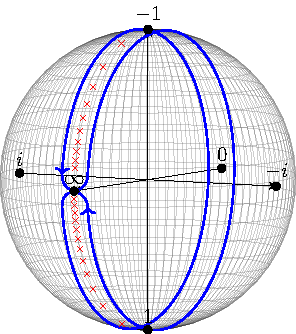
\includegraphics{thermal_field_theory/plots/integral_cont.pdf}        
    \end{subfigure}
    \begin{subfigure}{0.18\textwidth}
        \centering
        \begin{tikzpicture}
            \draw[-stealth] (0, 0) -- (1, 0);
        \end{tikzpicture}
        \end{subfigure}
    \begin{subfigure}{0.4\textwidth}
        \centering
        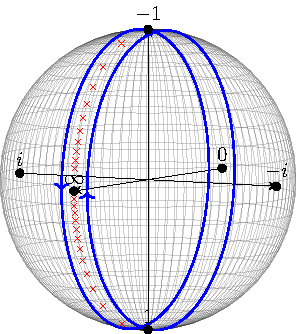
\includegraphics{thermal_field_theory/plots/integral_cont2.pdf}
    \end{subfigure} 
    \caption{The integral contour $\gamma$, and the result of deforming it into to contours close to the real line.
    The red crosses illustrate the poles of $n_B$.}
    \label{fig:integral contours}
\end{figure}

In the second line, we have changed variables $z \rightarrow -z$ in the first integral, and exploited the property $n_B(-i z) = -1 - n_B(iz)$.
In the last line, we use the assumption that $f(z)$ is analytic on the real line, and therefore also in a neighborhood of it. 
This allows us to shift the first integral back to the real line.
As $n_B(iz)$ is analytic outside the real line, the result of the second integral is the sum of residues of $f(z) + f(-z)$ in the lower half-plane.
The function
\begin{equation}
    f(z) 
    = \frac{1}{(z + i \mu)^2 + \omega^2} 
    = \frac{i}{2 \omega } 
    \left(
        \frac{1}{z + i(\mu + \omega)} - \frac{1}{z + i(\mu - \omega)}
    \right)
\end{equation}
obeys the assumed properties, as it has poles at
$z = - i (\mu \pm \omega)$, with residue $1 /( 2 \omega)$, so the function defined in \autoref{i func} may be written
\begin{equation}
    i(\omega, \mu) 
    = \frac{1}{2\omega}
    [1 + n_B(\omega - \mu) + n_B(\omega + \mu)].
\end{equation}

Using the antiderivative of the Bose distribution,
\begin{equation}
    \dv{\omega} \ln(1 - e^{-\beta \omega}) = \beta n_B(\omega),
\end{equation}
we get the final form of \autoref{j func}
\begin{equation}
    j(\omega, \mu) = \int \dd \omega'\, \omega' i(\omega', \mu)
    =  
    \frac{1}{2}\omega + \frac{1}{2\beta} 
    \left[
        \ln\left(1 - e^{-\beta(\omega - \mu)}\right)
        + \ln\left(1 - e^{-\beta(\omega + \mu)}\right)
    \right]
    + g'(\beta).
\end{equation}
The extra $\omega$-independent term $g'(\beta)$ is an integration constant.
We see there are temperature dependent terms, one due to the particle and one due to the anti-particle, and one due to the antiparticle, as they have opposite chemical potentials.

We now consider the sum over fermionic frequencies, which we for clarity denote $\tilde \omega_n$ in this chapter.
The procedure, in this case, is the same, except that we have to use a function with poles at the fermionic Matsubara frequencies.
This is done by the Fermi distribution, $n_F(z)$.
The Fermi distribution is
\begin{equation}
    n_F(\omega) = \frac{1}{e^{\beta \omega} + 1}.
\end{equation}
It obeys
\begin{align}
    &\odv{}{\omega} \ln(1 + e^{-\beta \omega}) = - \beta n_F(\omega), \\
    & n_F(- i\omega) = 1 - n_F(i\omega).
\end{align}
% The two distributions are related by
% \begin{equation}
%     2 n_B(i \omega; 2\beta) - n_B(i \omega; \beta)
%     = - n_F(i \omega; \beta ).
% \end{equation}
With this, the sum over fermionic Matsubara frequencies gives
\begin{align}
    \frac{1}{\beta} \sum_{\tilde \omega_n} f(\tilde \omega_n)
    & = \left(
        \int_{\infty + i \epsilon}^{-\infty + i \epsilon} \frac{\dd z}{2 \pi} 
        + \int_{-\infty - i \epsilon}^{\infty - i \epsilon}\frac{\dd z}{2 \pi}
    \right) 
    f(z) n_B(i z) \\
    & =
    \int_{-\infty}^{\infty} \frac{\dd z}{2 \pi} f(z)
    -
    \int_{-\infty - i \epsilon}^{\infty - i \epsilon}\frac{\dd z}{2 \pi}
    \left[
        f(z) - f(-z)
    \right]
    n_F(iz),
\end{align}
and 
\begin{equation}
    i(\omega, \mu) = \frac{1}{2 \omega} [1 - n_F(\omega - \mu) - n_F(\omega + \mu)].
\end{equation}
Using the antiderivative of the Fermi-distribution, we get
\begin{equation}
    j(\omega, \mu) 
    = \frac{1}{2} \omega 
    + \frac{1}{2 \beta }
    \left[
        \ln\left(1 + e^{-\beta(\omega - \mu)}\right)
        + \ln\left(1 + e^{-\beta(\omega + \mu)}\right)
    \right].
\end{equation}


    \section{*Interacting scalar field}
\label{section: interacting scalar}


We now study a scalar field with a $\lambda \varphi^4$ interaction term.
We write the Lagrangian in the form
%
\begin{equation}
    \Ell = \Ell^{(0)} + \Ell^{(I)}, \quad 
    \Ell^{(0)} = 
    \frac{1}{2} \partial_\mu \varphi \partial^\mu \varphi - m^2 \varphi^2 , \quad
    \Ell^{(I)} = - \frac{\lambda}{4!} \varphi^4.
\end{equation}
%
$\Ell^{(I)}$ is called the interaction term and makes it impossible to exactly solve for the partition function.
Instead, we turn to perturbation theory.
The canonical partition function in this theory is
%
\begin{equation}
    Z = \Tr{e^{- \beta \hat H}}
    = \int_S \D \varphi \, \exp{
        - \int_\Omega \dd X \left(\Ell_E^{(0)} + \Ell_E^{(I)}\right)
    }
    = \int_S \D \varphi \, e^{-S_0} e^{-S_I}.
\end{equation}
%
Here, $S_0$ and $S_I$ denote the Euclidean action due to the free and interacting Lagrangian, respectively.
The domain of integration $S$ is again periodic field configurations $\varphi(\beta, \vec x) = \varphi(0, \vec x)$.
We may write the free energy as
%
\begin{equation}
    - \beta F = \ln
    \left[
        \int_S \D \varphi \, e^{-S_0} \sum_n \frac{1}{n!} {(-S_I)}^n
    \right]
    = \ln Z_0 
    + \ln Z_I ,
\end{equation}
%
where $Z_0$ is the partition function of the free theory.
The correction to the partition function is thus given by
%
\begin{equation}
    Z_I = \sum_{n=0}^\infty \frac{(-1)^n}{n!} \ex{{S_I}^n}_0,
\end{equation}
%
where
%
\begin{equation}
    \ex{A}_0 = \frac{
        \int_S \D \varphi \, A \, e^{-S_0} }
    {\int_S \D \varphi \, e^{-S_0}}.
\end{equation}
%
To evaluate expectation values of the form $\ex{\varphi(X_1) ... }_0$, we introduce the partition function with a source term
%
\begin{align}
    Z[J] = \int_S \D \varphi \, \exp{
        - \frac{1}{2} \int_\Omega \dd X \, \varphi (-\partial_E^2 + m^2) \varphi
        + \int_\Omega \dd X \, J \varphi
    }.
\end{align}
%
Thermal propagators are the generalization of the time-ordered two-point functions $\ex{T\{\varphi(x) \varphi(y) \}}$ of the vacuum formalism.
For some differential operator $D^{-1}$, the thermal propagator is defined as
%
\begin{equation}
    D^{-1} D(X, Y) = \beta \delta(X - Y).
\end{equation}
%
The Fourier transformed propagator is, assuming $D(X, Y) = D(X-Y, 0)$,
%
\begin{align}
    \nonumber
    \tilde D(K, K') 
    & = \frac{1}{V \beta^3} \int_{\Omega} \dd X \dd Y \, 
    D(X, Y) \exp{- i [X\cdot K + Y\cdot K']} \\ \nonumber
    & = \frac{1}{V \beta^3} \int_{\Omega} \dd X' \dd Y' \, D(X', 0) 
    \exp{- i [X'\cdot \frac{1}{2} (K - K') + Y \cdot (K + K')] } \\
    & = \frac{1}{V \beta^2} \tilde D(K) \delta(K + K'),
\end{align}
where
%
\begin{equation}
    \tilde D(K) = \int \dd X e^{iK\cdot X} D(X, 0).
\end{equation}
%
We write the thermal propagator of the free field as $D_0(X, Y)$.
With this, we may complete the square,
%
\begin{align}
    Z[J] = Z[0]
    \exp{\frac{1}{2} \int_{\Omega} \dd X \dd Y J(X) D_0(X, Y) J(Y)}
    = Z[0] \exp{W[J]}.
\end{align}
We can now write
%
\begin{equation}
    \ex{\varphi(X)\varphi(Y)}_0 
    = \frac{1}{Z[0]}
    \frac{\delta}{\delta J(X)} \frac{\delta}{\delta J(Y)} 
    Z[J] \Big|_{J=0} 
    = D_0(X, Y).
\end{equation}
%
This generalizes to higher-order expectation values,
%
\begin{equation}
    \ex{\varphi(X_i) \dots \varphi(X_n)}_0
    = \frac{1}{Z[0]} \left(\prod_{i=1}^n \frac{\delta}{\delta J(X_i)}\right) 
    Z[J] \Big|_{J=0},
\end{equation}
%
Using Wick's theorem, as described in \autoref{section: path integral}, the expectation values we are evaluating can be written
%
\begin{align*}
    \ex{{S_I}^m}_0 & 
    = \left(- \frac{\lambda }{4!}\right)^m 
    \int_{\Omega} \dd X_1 \dots \dd X_m
    \ex{\varphi^4(X_1) \dots \varphi^4(X_m)}_0 \\ 
    & 
    = \left(- \frac{\lambda }{4!}\right)^m 
    \int_{\Omega} \dd X_1 \dots \dd X_m \sum_{\{a, b\}}
    \ex{\varphi(X_{a(1)}) \varphi(X_{b(1)})}_0
    \dots
    \ex{\varphi(X_{a(2m)}) \varphi(X_{b(2m)})}_0,
\end{align*}
%
where $X_i$ for $i>m$ is defined to equal $X_j$, where $j = i \mod m$.
More simpliy,  $X_{m + i} = X_i$.
The functions $a,\,b$ represents a possible pairing, as described in \autoref{section: path integral}.
Inserting the Fourier expansions of the field gives
%
\begin{align*}
    \ex{{S_I}^m}_0
    &\quad 
    = \left(-\frac{\lambda }{4!}\right)^m 
    \int_{\Omega} \dd X_1 \dots \dd X_m
    (V \beta)^2 \int_{\tilde \Omega} \dd K_1 \dots \dd K_{2m} \sum_{\{a, b\}}
    \exp{i {\sum}_{i=1}^{m} X_i \cdot K_i}
    \\ & \quad \quad \quad \quad\quad \quad \quad \quad
    \times \ex{\varphi(K_{a(1)}) \varphi(K_{b(1)})}_0
    \dots
    \ex{\varphi(K_{a(2m)}) \varphi(K_{b(2m)})}_0     
    \\ \\ & \quad  
    = \left(-\frac{\lambda }{4!}\right)^m 
    \frac{(V \beta)^{2m} \beta^m}{(V \beta^2)^{2m}}
    \int_{\tilde \Omega} \dd K_1 ... \dd K_{2m} \sum_{\{a, b\}}
    \prod_{i=1}^m \delta\left({\sum}_{j=0}^3 K_{i + jm}\right) \\
    & \quad \quad \quad \quad \quad \quad \quad \quad \quad \quad \quad
    \times \tilde D(K_{a(1)}) \delta(K_{a(1)} + K_{b(1)}) \dots 
    \tilde D(K_{a(2m)}) \delta(K_{a(2m)} + K_{b(2m)})
    \\ \\ & \quad 
    = \left(-\frac{\lambda \beta}{4!}\right)^m 
    \prod_{i=1}^{2m} \int_{\tilde \Omega} 
    \left( \dd K_i \frac{1}{\beta} \tilde D(K_i)  \right) 
    \prod_{i=1}^m \delta\left({\sum}_{j=0}^3 K_{i + jm}\right)
    \sum_{\{a, b\}} 
    \prod_{n=1}^{2m}\delta(K_{a(k)} + K_{b(k)}).
\end{align*}
%
Here we have used that $V \beta^2 \tilde D_0(K, P) = \tilde D_0(K) \delta(P + K)$, where $\tilde D_0(K)$ is the thermal propagator for the free field.
In this case, it is
%
\begin{equation}
    \tilde D_0(K) = \tilde D_0(\omega_n, \vec k) = \frac{1}{\omega_k^2 + \omega_n^2}.
\end{equation}
%
This expectation value can be represented graphically using Feynman diagrams.
The thermal $\lambda \varphi^2$-theory gets the prescription
%
\begin{align}
    \feynmandiagram[small, horizontal=a to b, baseline=(c)]{
        a --[fermion, edge label'=$K_1$] c[dot] --[anti fermion,edge label=$K_4$] d, 
        b--[fermion, edge label=$K_2$]c--[anti fermion, edge label'=$K_3$]e,
    };
    & = -\lambda \beta
    \delta \left({\sum}_i K_i \right), \\ \nonumber \\
    \feynmandiagram[horizontal=a to b, baseline=(a)]{a --[fermion, edge label=$K$] b};
    & = \frac{1}{\beta} D_0(K).
\end{align}
%
Lastly, one has to integrate over internal momenta and divide by the symmetry factor of the diagram $s$, which is described in detail in~\autocite{peskinIntroductionQuantumField1995}.
%
Calculating $\ex{{S_I}^n}_0$ boils down to the sum of all possible Feynman diagrams with $n$ vertices.
The first example is 
%
\begin{align}
    \ex{S_I}_0 =
    \frac{1}{8}\,
    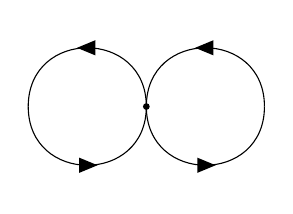
\begin{tikzpicture}[baseline=(c)]
    \begin{feynman}
        \vertex (a) at (0, 0);
        \vertex (b) at (1.5, 0);
        \vertex (c) at (3, 0);
        \filldraw[black] (b) circle (1pt);
        \diagram*{
            {[edges=fermion]
            (a)--[half right, looseness=1.7] (b)--[half right, looseness=1.7](a),
            (b)--[half right, looseness=1.7] (c)--[half right, looseness=1.7](b),
        }};
    \end{feynman}
    \end{tikzpicture}.
\end{align}
%
In \autoref{section: path integral}, we saw that the sum of all vacuum diagrams is the exponential of the sum of all \emph{connected} diagrams.
If we include a rule of dividing diagrams by factor $\beta V$, then the free energy density of the interacting theory is given by
%
\begin{equation}
    \Eff 
    = - \frac{\ln Z_0}{V\beta} 
    + \sum  \left( \mathrm{all\,\, connected\,\, diagrams}\right).
\end{equation}
%
    \section{*Fermions}
\label{section: fermions}


The derivation of the fermionic path integral is similar to the scalar one, but with some slight but important differences.
If $\psi$ and $\bar \psi$ are fermionic spinor fields, relevant relations are~\autocite{laineBasicsThermalField2016}
%
\begin{align}
    \one 
    &=
    \int \D \psi \D \bar \psi \,
    \exp{- \int \dd X \, \bar \psi \psi}
    \ket{\psi} \bra{\psi} \\
    \braket{\bar \psi | \psi } 
    &= \exp{\int \dd X\, \bar \psi \psi}\\
    Z 
    &= \Tr{\hat \rho} 
    = \int \D \psi \D \bar \psi\,
    \exp{- \int \dd X \, \bar \psi \psi} \braket{- \psi | e^{i\beta \hat H} | \psi},
\end{align}
%
The anti-periodic nature of fermion-fields, as mentioned in \autoref{section: imaginary-time formalism}, is due to these differences.
We can verify them by studying the properties of the thermal Greens function.
The thermal Greens function may be written 
\begin{equation}
    D(X_1, X_2) = D(\vec x, \vec y, \tau_1, \tau_2) 
    = \Tr{e^{-\beta H} \psi(\tau_1, \vec x)\psi(\tau_2, \vec y) }.
\end{equation}
In the same way that $i \hat H$ generates the time translation of a quantum field operator through 
$
\hat\varphi(x) = \hat\varphi(t, \vec x) = e^{it\hat H} \hat \varphi(0, \vec x) e^{-it\hat H} 
$, 
the imaginary-time formalism implies the relation
$
    \hat\varphi(X) = \hat\varphi(\tau, \vec x) 
    = e^{\tau\hat H} \hat \varphi(0, \vec x) e^{-\tau \hat H}.
$
Using $\one = e^{\tau \hat H} e^{-\tau \hat H}$ and the cyclic property of the trace, we show that, assuming $\beta>\tau>0$,
\begin{align*}
    D(\vec x, \vec y, \tau, 0)
    % = \bra{\Omega}e^{-\beta \hat H} \T{\varphi(\tau, \vec x) \varphi(0, \vec y)}\ket{\Omega} 
    &= \frac{1}{Z} \Tr{
        e^{-\beta \hat H} \varphi(\tau, \vec x) \varphi(0, \vec y)
    } \\
    % & = \frac{1}{Z} \Tr{
    %     \varphi(0, \vec y) e^{-\beta \hat H} \varphi(\tau, \vec x)
    % } \\
    & = \frac{1}{Z} \Tr{
        e^{-\beta \hat H} e^{\beta \hat H} \varphi(0, \vec y) 
        e^{-\beta \hat H} \varphi(\tau, \vec x)
    } \\
    & = \frac{1}{Z} \Tr{
        e^{-\beta \hat H} \varphi(\vec y, \beta) \varphi(\tau, \vec x)
    } 
    = \nu D (\vec x, \vec y, \tau, 0)
    % = \nu \bra{\Omega}        
    % e^{-\beta \hat H} \T{ \varphi(\tau, \vec x) \varphi( \beta, \vec y) }
    % \ket{\Omega}.
\end{align*}
This implies that $\varphi(0, x) = \nu \varphi(\beta, \varphi)$, where $\nu = \pm 1$ for bosons and fermions respectively, which shows that bosons are periodic in time, as stated earlier, while fermions are anti-periodic.


The Lagrangian density of a free fermion is
\begin{equation}
    \Ell = \bar \psi \left( i \slashed{\partial} - m \right) \psi.
\end{equation}
This Lagrangian is invariant under the transformation $\psi \rightarrow e^{-i \alpha} \psi$, which by Nöther's theorem results in a conserved current
\begin{equation}
    j^\mu = \pdv{\Ell}{(\partial_\mu \psi)} \delta \psi=  \bar \psi \gamma^\mu \psi.
\end{equation}
The canonical momentum corresponding to $\psi$ is
\begin{equation}
    \pi = \pdv{\Ell}{(\partial_0 \psi)} = i \bar \psi \gamma^0,
\end{equation}
and the Hamiltonian density is 
\begin{equation}
    \He = \pi \dot\psi - \Ell
    = \bar \psi (-i\gamma^i\partial_i + m) \psi
\end{equation}
%
In the grand canocical ensamble, we substitute $\He \rightarrow \He - \mu \bar \psi \gamma^0 \psi$, which gives the euclidian Lagrangian
which gives
%
\begin{equation}
    \Ell_E = 
    - \pi \dot\psi + \He(\psi, \pi) - \mu \bar \psi \gamma^0 \psi
    = \bar\psi[\gamma^0 (\partial_\tau - \mu) - i\gamma^i \partial_i + m] \psi,
\end{equation}

With this, the partition function is
%
\begin{align*}
    Z & = \int \D \psi \D \bar \psi
    \exp{
        - \int_\Omega \dd X \, \bar \psi
        \left[
            \gamma_0(\partial_\tau -\mu) -  i \gamma^i \partial_i + m
        \right]
        \psi
    }\\
    % & = C \int \D \tilde \psi\D \tilde {\bar \psi}\,
    % \exp{
    %     - \int_{\tilde \Omega} \dd K \, \tilde {\bar \psi}
    %     \left[
    %         i \gamma_0(\omega_n + i\mu) + i \gamma_i p_i + m
    %     \right]
    %     \tilde \psi
    % } \\
    & = C \int \D \tilde \psi \D \tilde {\bar \psi} \,
    e^{- \langle \tilde {\bar \psi}, D^{-1} \tilde \psi\rangle} 
    = \det(D^{-1}).
\end{align*}
In the second line, we have inserted the Fourier expansion of the field, as defined in \autoref{section: imaginary-time formalism}, and changed variable of integration, as we did for the scalar field.
We then used the Grassmann version of the Gaussian integral,~\autocite{schwartzQuantumFieldTheory2013}
%
\begin{equation}
    \int \dd \bar \theta_i \dd \theta_i \exp{- \theta_i A_{ij}\theta_j} = \det(A).
\end{equation}
%
The linear operator in this case is 
\begin{equation}
    D^{-1} = i \gamma^0 (-i\partial_\tau + i\mu) - (- i \gamma^i) \partial_i + m
    = 
    \beta [i \tilde \gamma_a k_a + m ].
\end{equation}
This equality must be understood as an equality between linear operators, which are represented in different bases.
We introduced the notation $k_a = (\omega_n + i \mu, k_i)$ and use the Euclidean gamma matrices $\tilde \gamma_i$, as defined in \autoref{subsection: Pauli matrices}.
We use the fact that
%
\begin{equation*}
    \det(i\tilde\gamma_a k_a + m)
    = \det(\gamma^5 \gamma^5)
    \det(i\tilde\gamma_a k_a + m)
    = \det[\gamma^5 (i\tilde\gamma_a k_a + m) \gamma^5]
    = \det(-i\tilde\gamma_a k_a + m),
\end{equation*}
%
Let $\tilde D^{-1} = \beta[-i\tilde\gamma_a k_a + m]$, which means we can write
%
\begin{equation}
    Z = \sqrt{\det(D^{-1})\det(\tilde D^{-1})} = \sqrt{\det(D^{-1}\tilde D^{-1})} 
    = \det[\one \beta^2(k_a k_a + m^2)]^{1/2},
\end{equation}
%
where we have used the anti-commutation rule for the Euclidean gamma-matrices, $\{\tilde \gamma_a, \tilde  \gamma_b\} = 2 \delta_{ab}$.
It is important to keep in mind that the determinant here refers to linear operators on the space of spinor functions.
Thus
%
\begin{align}
    \nonumber
    \ln(Z) 
    & = \ln\left\{\det[\one\beta^2(k_a k_a + m^2)]^{1/2}\right\}
    = \frac{1}{2} \Tr{\ln[\one\beta^2(k_a k_a + m^2)]} \\
    & =  2 \int_{\tilde \Omega} \dd K \,  \ln\{ \beta^2[(\omega_n + i\mu)^2 + \omega_k^2]\}.
\end{align}
%
In the last step, we used the fact that the matrix within the logarithm is diagonal.
The matrix part of the trace is trivial and therefore trivial.
Using the fermionic version of the thermal sum from \autoref{section: thermal sum} gives the answer
%
\begin{equation}
    \label{free energy fermions}
    \Eff 
    = -\frac{2}{\beta} \int\frac{\dd^3 k}{(2\pi)^3} \, 
    \left[
        \beta \omega_k
        + \ln\left(1 + e^{-\beta(\omega_k-\mu)}\right)
        + \ln\left(1 + e^{-\beta(\omega_k+\mu)}\right)
    \right].
\end{equation}
%
We see again that the temperature-independent part of the integral diverges, and must be regulated.
There are two temperature-dependent terms, one from the particle and one from the anti-particle.


    
    \chapter{Code}
    \label{appendix: code} 
 
All code is available at: \url{https://github.com/martkjoh/master}.


\section{Integrating the TOV equations}

For numerical integration of the TOV equations, we use SciPy's \texttt{integrate.solve\_ivp}.\footnote{
    Reference available here: \url{https://docs.scipy.org/doc/scipy/reference/generated/scipy.integrate.solve_ivp.html}.
    }
Equations of state are evaluated either as explicit functions if a closed-form is available or as an interpolating function is created using a cubic spline without smoothing.
All code is written using dimensionless variables, and setting $k_1 = k_2 = k_3$.
The TOV equation is then \autoref{TOV dimensionless}
%
\begin{align}
    \odv{\tilde m}{\tilde r} 
    = 3 \tilde r^2 \tilde u, \quad
    \odv{\tilde p}{\tilde r} 
     = - \frac{1}{\tilde r^2} \left(\tilde p + \tilde u\right) 
    \left(3  \tilde r^3 \tilde p + \tilde m\right) 
    \left(1 - \frac{2 \tilde m}{\tilde r}\right)^{-1}.
\end{align}
%
As $r \rightarrow 0$, parts of the TOV equation \autoref{TOV dimensionless} approaches a $0/0$-limit, and we must make use of an approximation for numeric evaluation.
The Taylor-expansion of the mass function around $\tilde r = 0$ is
%
\begin{equation}
    \tilde m(r) = \tilde m(0) + \tilde m'(0) \, \tilde r + \frac{1}{2!} \tilde m''(0) \tilde r^2
    + \frac{1}{3!} \tilde m'''(0) \tilde r^3 + \Oh\left(\tilde r^4\right).
\end{equation}
%
One of the boundary conditions is $\tilde m(0) = 0$.
We then use the differential equation for $\tilde m$, \autoref{diff eq mass}, to find
%
\begin{equation}
    \tilde m'(0) = 0, \quad
    \tilde m''(0) = 0, \quad
    \tilde m'''(0) = 6 k_2 \tilde u_0,
\end{equation}
%
where $\tilde u_0 = \tilde u(r = 0)$.
We get an approximation of the TOV equation for $\tilde r \ll 1$ by substituting the $\tilde m$ for its Taylor expansion and including only the leading-order term, which gives
%
\begin{equation}
    \odv{\tilde p}{\tilde r}
    \sim - \tilde r \, \left(\tilde p + \tilde u\right)
    \left( 3 \tilde p + \tilde u_0  \right)
    \left(1 - 2 \tilde u_0 \tilde r^2\right)^{-1}, \quad r\rightarrow 0
\end{equation}
%
For the Newtonian approximation to the TOV equation, we get
%
\begin{equation}
    \odv{\tilde p}{\tilde r} = -\frac{\tilde u \tilde m}{\tilde r^2}
    \sim - \tilde u \tilde u_0 \tilde r,  \quad r\rightarrow 0.
\end{equation}

 


\section{Spherically symmetric metric}

The calculations in \autoref{chapter: GR} were done using a CAS system.
The code is written in Python in a Jupyter notebook.
The full \texttt{.ipynb} file with executable code is available in the repository, at \url{https://github.com/martkjoh/master/blob/main/scripts/TOV/TOV.ipynb}
Below is some of the code, which illustrates the main functions and the outputs.

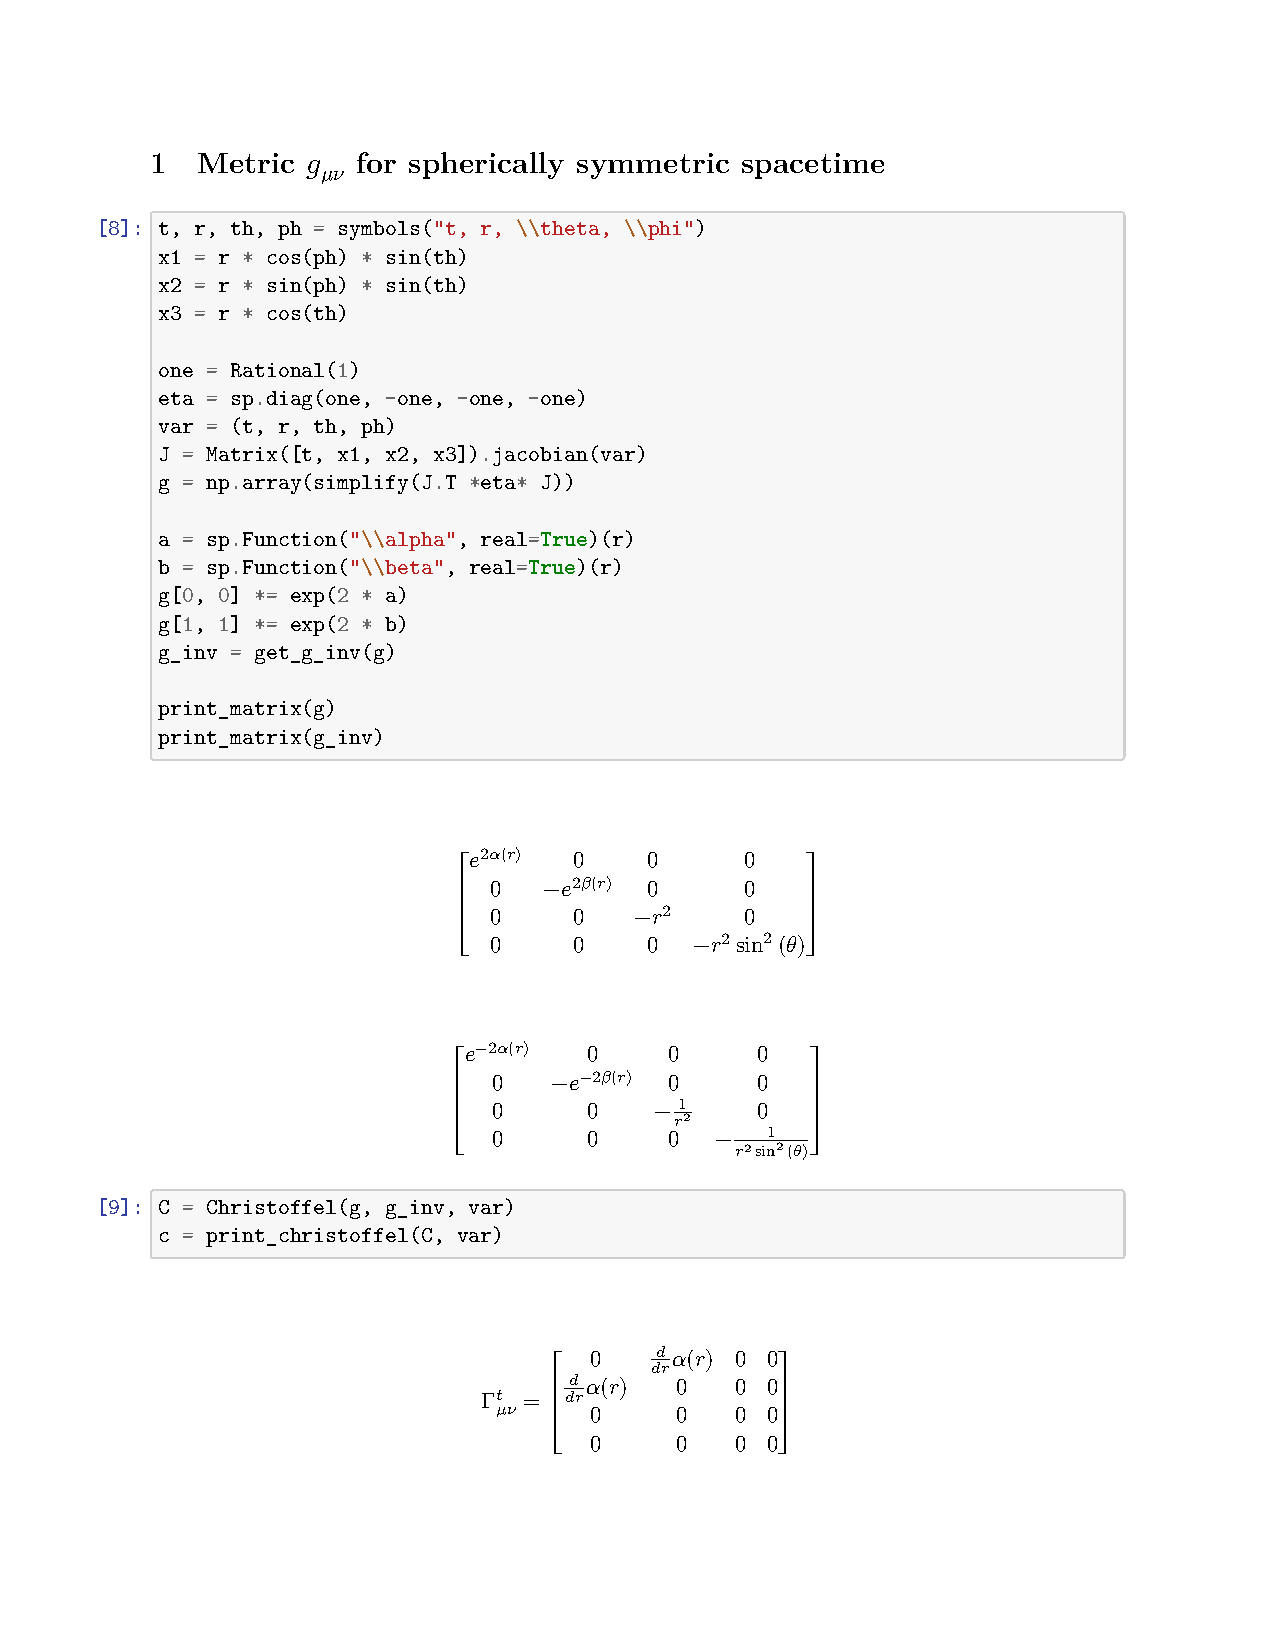
\includepdf[pages=-,pagecommand={},width=1.3\textwidth]{../scripts/TOV/TOV.pdf}




\section{Symbolic calculations in \chpt}
\label{section: symbolic calculations}

Symbolic calculations in \chpt, such as the expansion of the Lagrangian in $\varphi$, were done using the open-source, Python-based case SageMath\footnote{\url{https://www.sagemath.org/}}, and jupyter notebook\footnote{\url{https://jupyter.org/}}.
The calculations consisted of expanding the Lagrangian in a series of $\varphi_a/f$.
The calculations presented in this thesis, in addition to expansions of $\Ell_4$ to second order, can be found in the online repository, at \url{https://github.com/martkjoh/master/tree/main/power_expansion}.



    \cleardoublepage
    \phantomsection
    \addcontentsline{toc}{chapter}{Bibliography}
    \printbibliography

\end{document}
